\section{Casi d'Uso}

\subsection{Attori}
Gli attori individuati sono distinti in primari, che avviano l'interazione con il sistema, e secondari, ovvero sistemi esterni che forniscono o ricevono servizi dal sistema.

\begin{itemize}
    \item \textbf{Mittente}: attore primario. Rappresenta il cliente B2B, identificato tramite anagrafica, che invia richieste non strutturate attraverso i canali monitorati. Il sistema opera in modo autonomo: le fasi della pipeline sono quindi modellate come casi d'uso innescati dalla richiesta del mittente, che non interagisce direttamente con l'interfaccia (VE-1.1, VE-1.4, LG-1.1).
    \item \textbf{Utente non autenticato}: attore primario. Chiunque acceda all'interfaccia amministrativa senza essersi ancora autenticato; dopo l'autenticazione assume il ruolo di Utente in sola lettura, Gestore o Amministratore in base al proprio profilo.
    \item \textbf{Utente in sola lettura}: attore primario. Utente dell'interfaccia amministrativa che consulta richieste, log e dashboard di monitoraggio, senza poter modificare la configurazione o i dati (LG-3.3, LG-4.2).
    \item \textbf{Gestore}: attore primario. Utente dell'interfaccia amministrativa che, oltre alle funzionalità dell'Utente in sola lettura, gestisce le regole di azione e notifica e le richieste non riuscite (LG-3.3).
    \item \textbf{Amministratore}: attore primario. Utente dell'interfaccia amministrativa che, oltre alle funzionalità del Gestore, configura canali, applicativi di destinazione, modello LLM, posta in uscita e soglia di confidenza, gestisce anagrafica, utenti e profili e la persistenza dei dati (LG-3.3).
    \item \textbf{Canale di ingresso}: attore secondario (sistema esterno). Sorgente da cui il sistema acquisisce le richieste: casella di posta elettronica, canale WhatsApp o, come funzionalità desiderabile, cartella del filesystem, locale o remota (VE-1.1, LG-1.1).
    \item \textbf{Motore di estrazione (OCR / Speech-to-Text)}: attore secondario (sistema esterno). Componente che converte in testo audio, immagini e documenti scansionati, ad esempio Whisper, Google Speech, Tesseract o EasyOCR (VE-1.2, LG-1.1).
    \item \textbf{LLM}: attore secondario (sistema esterno). Fornisce i servizi di raffinamento dell'estrazione, individuazione dell'intenzione, estrazione delle entità e strutturazione dei dati tramite interfaccia compatibile con le API di OpenAI; è un modello a pesi aperti eseguito in locale, ad esempio Qwen (VE-1.8, LG-2.1, LG-2.2).
    \item \textbf{Applicativo aziendale di destinazione}: attore secondario (sistema esterno). Portale B2B, ERP, CRM o sistema di ticketing che riceve i dati strutturati tramite API REST; in fase di sviluppo la proponente fornisce mock e API dedicate (VE-1.1, LG-2.3).
    \item \textbf{Servizio di posta in uscita}: attore secondario (sistema esterno). Servizio SMTP utilizzato per l'invio di notifiche e messaggi al mittente (Capitolato).
\end{itemize}

I casi d'uso sono numerati in modo gerarchico: \textbf{UC N.k} è un caso d'uso collegato a \textbf{UC N} tramite relazione di estensione o di inclusione. I fallimenti che rendono la richiesta non elaborabile includono \hyperref[uc:34]{UC 34}, che a sua volta include \hyperref[uc:37]{UC 37}.

% ------------------------------------------------------------
% MACROAREA 1 --- ACQUISIZIONE DELLE RICHIESTE DAI CANALI
% ------------------------------------------------------------
\subsection{Macroarea 1 --- Acquisizione delle richieste dai canali}

\subsubsection{UC 1: Acquisizione e-mail dalla casella monitorata}\label{uc:1}
\begin{center}
\captionsetup{type=figure}
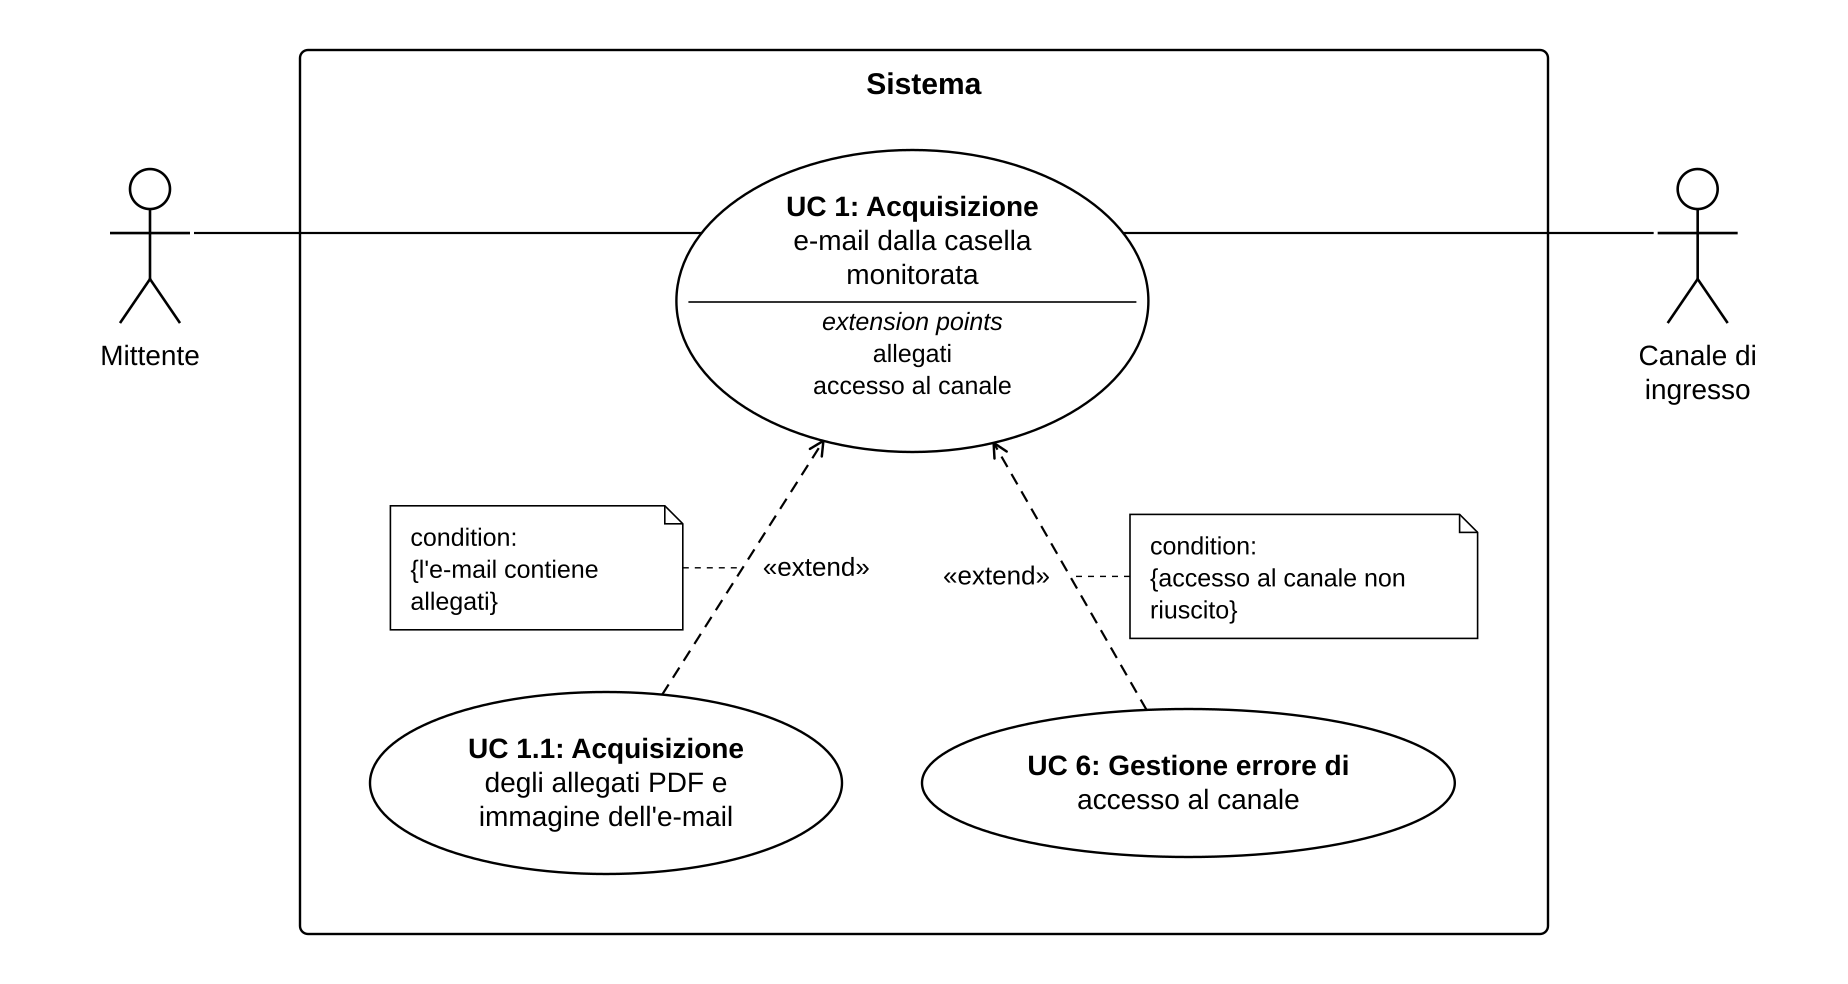
\includegraphics[width=\linewidth,height=0.32\textheight,keepaspectratio]{img/UC1.png}
\caption{UC 1 -- Acquisizione e-mail dalla casella monitorata}
\end{center}
\begin{itemize}
    \item \textbf{Attore principale}: Mittente
    \item \textbf{Attori secondari}: Canale di ingresso
    \item \textbf{Precondizioni}: Il canale e-mail è configurato e attivo e il sistema è in esecuzione.
    \item \textbf{Scenario principale}:
    \begin{enumerate}
        \item Il mittente invia un'e-mail alla casella monitorata.
        \item Il sistema rileva il nuovo messaggio.
        \item Il sistema acquisisce mittente, oggetto e testo del messaggio.
        \item Il sistema crea una richiesta associata al messaggio.
    \end{enumerate}
    \item \textbf{Postcondizioni}: La richiesta è acquisita ed è pronta per le fasi successive della pipeline.
    \item \textbf{Trigger}: Arrivo di un nuovo messaggio nella casella di posta monitorata.
    \item \textbf{Estensioni}:
    \begin{itemize}
        \item \hyperref[uc:1.1]{UC 1.1}: Acquisizione degli allegati PDF e immagine dell'e-mail $\rightarrow$ Condizione: L'e-mail contiene allegati.
        \item \hyperref[uc:6]{UC 6}: Gestione errore di accesso al canale $\rightarrow$ Condizione: Accesso al canale non riuscito.
    \end{itemize}
\end{itemize}

\subsubsection{UC 1.1: Acquisizione degli allegati PDF e immagine dell'e-mail}\label{uc:1.1}
\begin{center}
\captionsetup{type=figure}
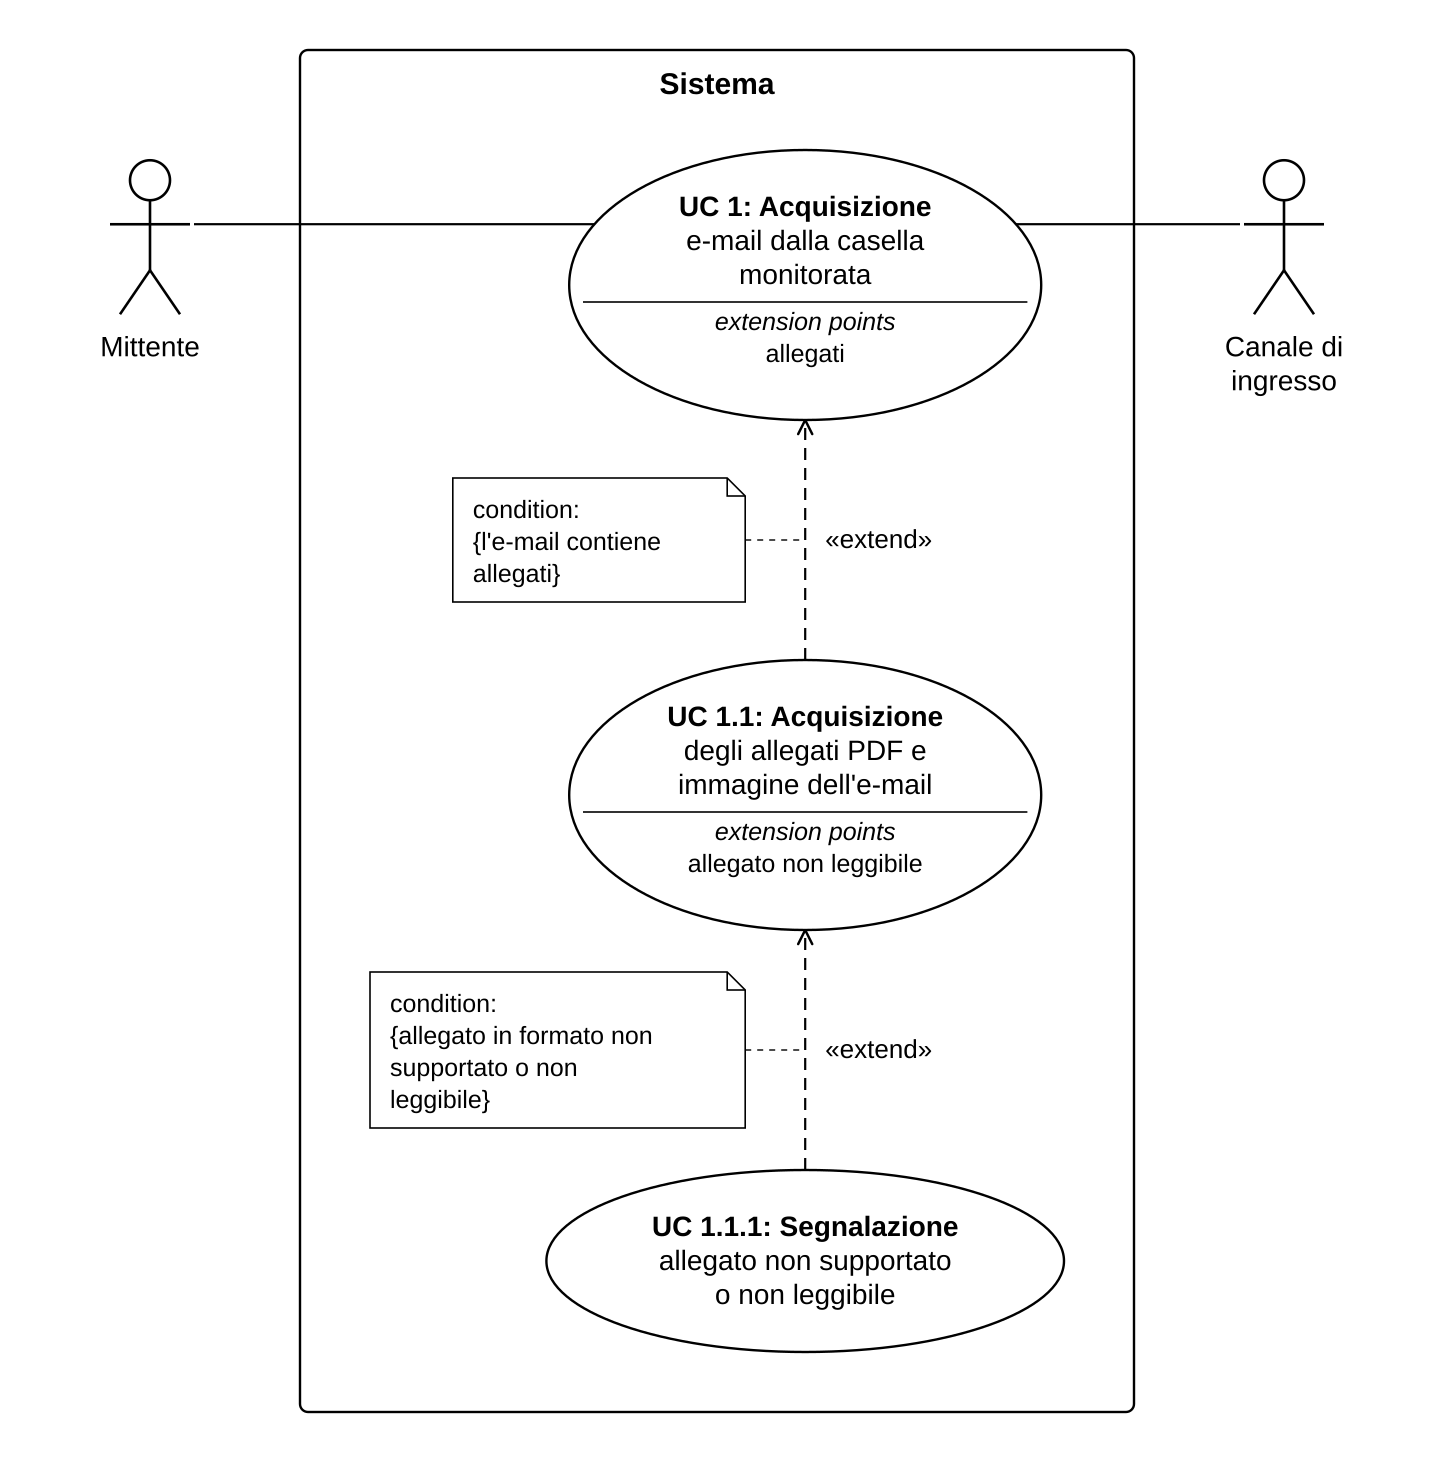
\includegraphics[width=\linewidth,height=0.32\textheight,keepaspectratio]{img/UC1_1.png}
\caption{UC 1.1 -- Acquisizione degli allegati PDF e immagine dell'e-mail}
\end{center}
\begin{itemize}
    \item \textbf{Attore principale}: Mittente
    \item \textbf{Precondizioni}: L'acquisizione di un'e-mail è in corso e il messaggio contiene allegati.
    \item \textbf{Scenario principale}:
    \begin{enumerate}
        \item Il sistema individua gli allegati del messaggio.
        \item Il sistema acquisisce gli allegati in formato PDF e immagine.
        \item Il sistema associa gli allegati alla richiesta.
    \end{enumerate}
    \item \textbf{Postcondizioni}: Gli allegati sono acquisiti e associati alla richiesta.
    \item \textbf{Trigger}: Presenza di allegati nell'e-mail acquisita.
    \item \textbf{Estende}: \hyperref[uc:1]{UC 1}.
    \item \textbf{Estensioni}:
    \begin{itemize}
        \item \hyperref[uc:1.1.1]{UC 1.1.1}: Segnalazione allegato non supportato o non leggibile $\rightarrow$ Condizione: Allegato in formato non supportato o non leggibile.
    \end{itemize}
\end{itemize}

\subsubsection{UC 1.1.1: Segnalazione allegato non supportato o non leggibile}\label{uc:1.1.1}
\begin{center}
\captionsetup{type=figure}
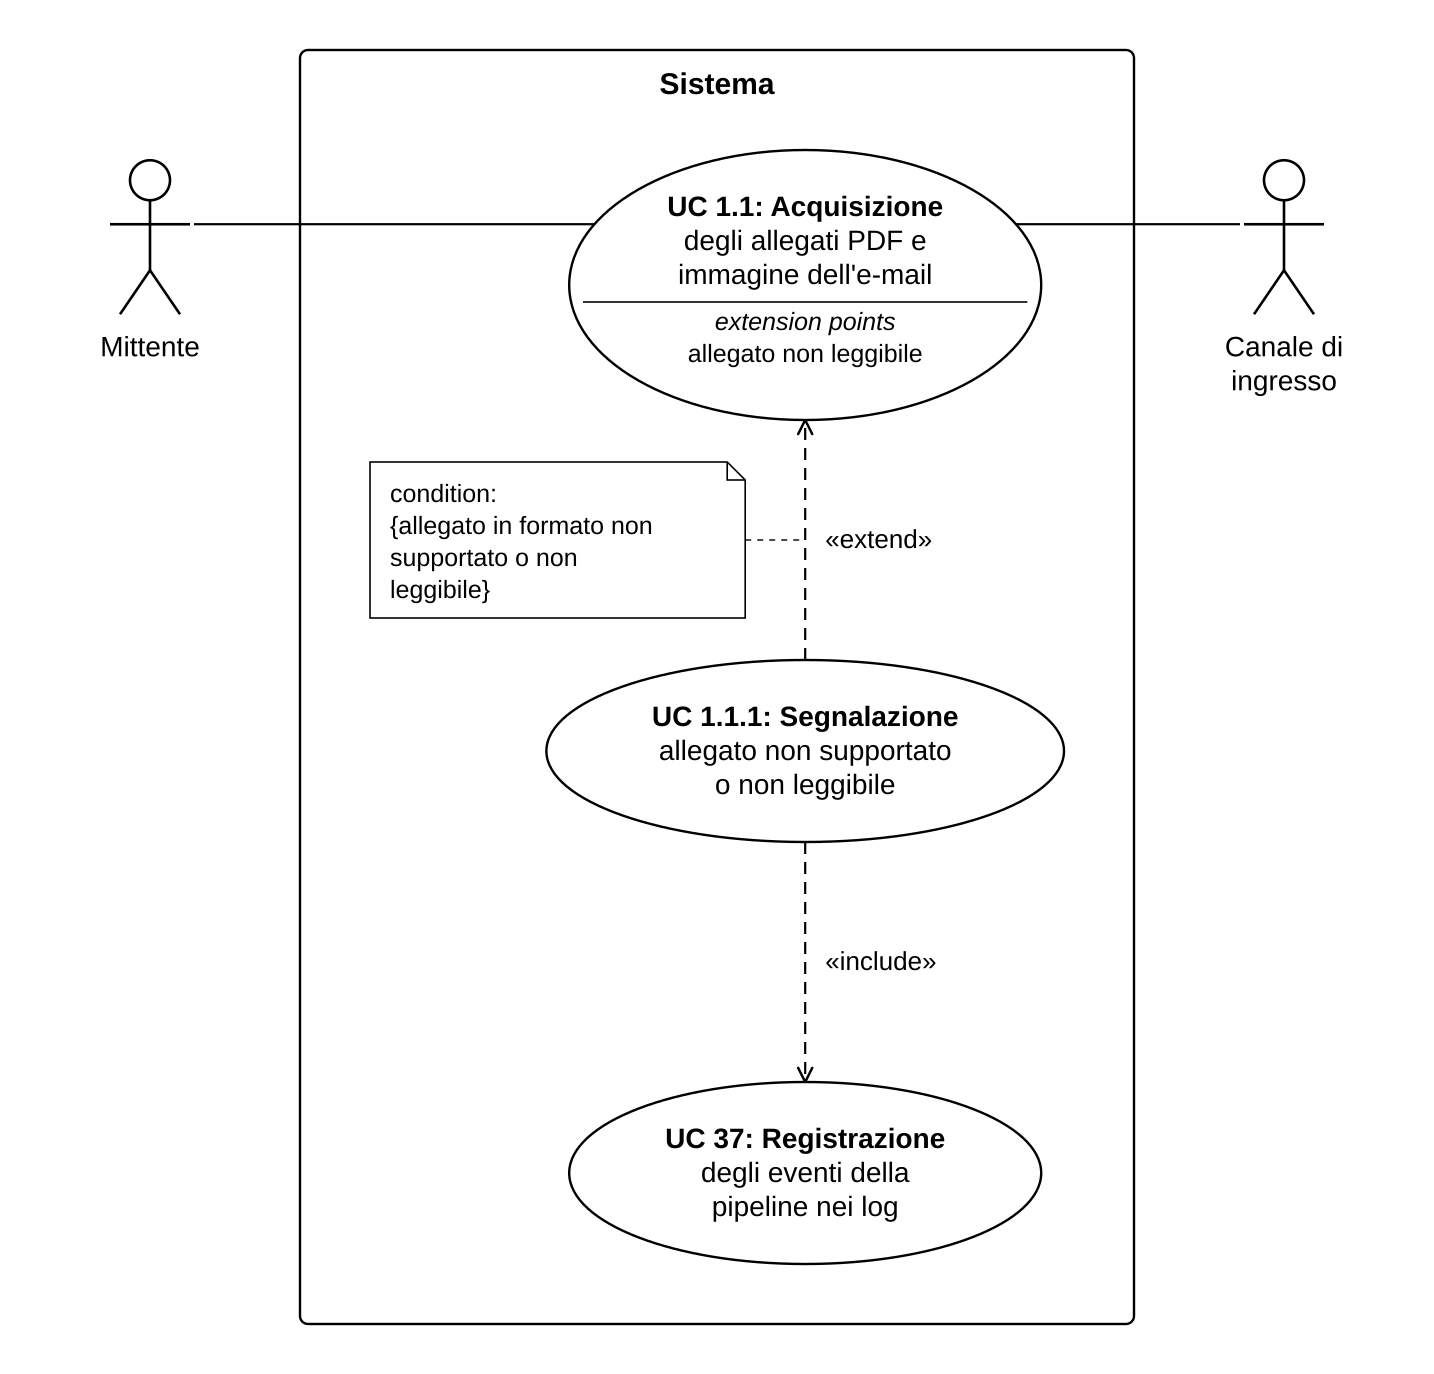
\includegraphics[width=\linewidth,height=0.32\textheight,keepaspectratio]{img/UC1_1_1.png}
\caption{UC 1.1.1 -- Segnalazione allegato non supportato o non leggibile}
\end{center}
\begin{itemize}
    \item \textbf{Attore principale}: Mittente
    \item \textbf{Precondizioni}: L'acquisizione degli allegati è in corso.
    \item \textbf{Scenario principale}:
    \begin{enumerate}
        \item Il sistema rileva un allegato in formato non supportato o non leggibile.
        \item Il sistema marca la richiesta come non riuscita (\hyperref[uc:34]{UC 34}).
        \item Il sistema registra l'anomalia nei log (\hyperref[uc:37]{UC 37}).
    \end{enumerate}
    \item \textbf{Postcondizioni}: La richiesta è marcata come non riuscita e l'anomalia è registrata nei log.
    \item \textbf{Trigger}: Allegato in formato non supportato o non leggibile.
    \item \textbf{Estende}: \hyperref[uc:1.1]{UC 1.1}.
    \item \textbf{Inclusioni}:
    \begin{itemize}
        \item \hyperref[uc:34]{UC 34}: Marcatura della richiesta come non riuscita
    \end{itemize}
\end{itemize}

\subsubsection{UC 2: Acquisizione messaggio vocale WhatsApp}\label{uc:2}
\begin{center}
\captionsetup{type=figure}
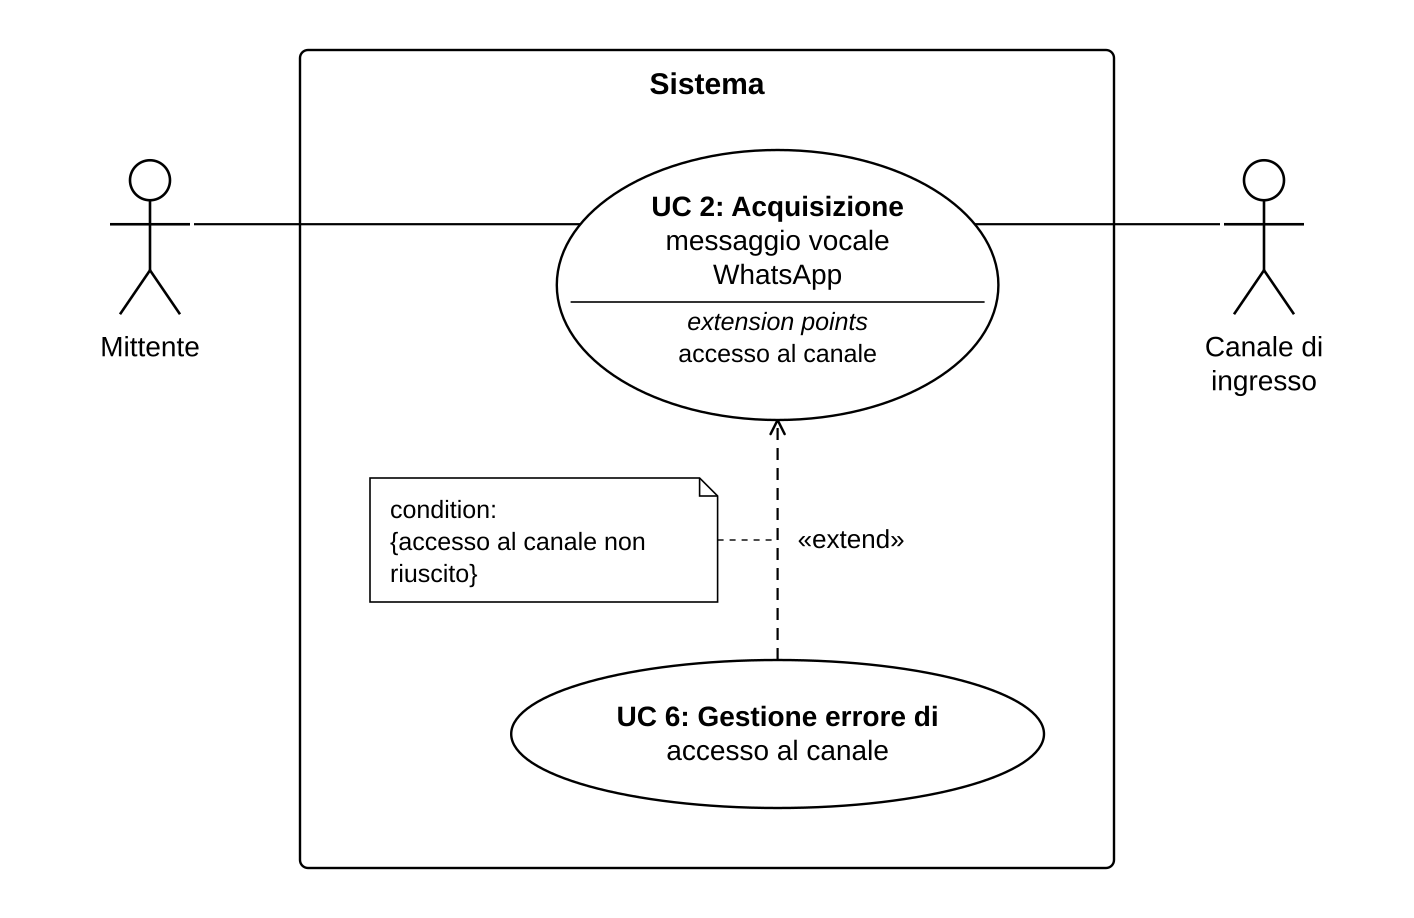
\includegraphics[width=\linewidth,height=0.32\textheight,keepaspectratio]{img/UC2.png}
\caption{UC 2 -- Acquisizione messaggio vocale WhatsApp}
\end{center}
\begin{itemize}
    \item \textbf{Attore principale}: Mittente
    \item \textbf{Attori secondari}: Canale di ingresso
    \item \textbf{Precondizioni}: Il canale WhatsApp è configurato e attivo e il sistema è in esecuzione.
    \item \textbf{Scenario principale}:
    \begin{enumerate}
        \item Il mittente invia un messaggio vocale al canale WhatsApp monitorato.
        \item Il sistema rileva il nuovo messaggio.
        \item Il sistema acquisisce il numero del mittente e il file audio.
        \item Il sistema crea una richiesta associata al messaggio.
    \end{enumerate}
    \item \textbf{Postcondizioni}: La richiesta è acquisita con il file audio ed è pronta per la trascrizione.
    \item \textbf{Trigger}: Arrivo di un messaggio vocale sul canale WhatsApp.
    \item \textbf{Estensioni}:
    \begin{itemize}
        \item \hyperref[uc:6]{UC 6}: Gestione errore di accesso al canale $\rightarrow$ Condizione: Accesso al canale non riuscito.
    \end{itemize}
\end{itemize}

\subsubsection{UC 3: Acquisizione messaggio testuale WhatsApp}\label{uc:3}
\begin{center}
\captionsetup{type=figure}
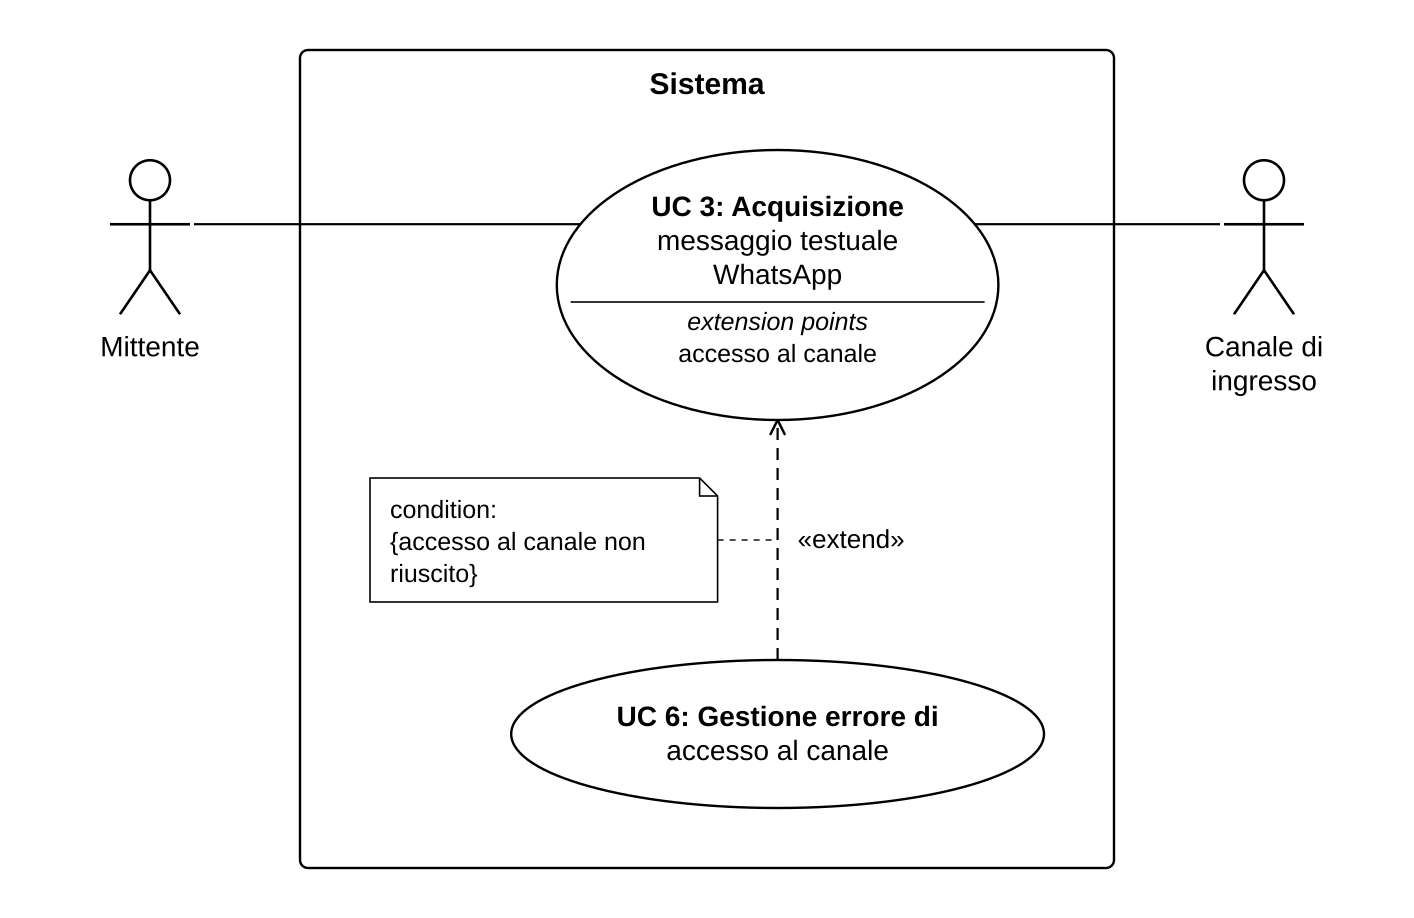
\includegraphics[width=\linewidth,height=0.32\textheight,keepaspectratio]{img/UC3.png}
\caption{UC 3 -- Acquisizione messaggio testuale WhatsApp}
\end{center}
\begin{itemize}
    \item \textbf{Attore principale}: Mittente
    \item \textbf{Attori secondari}: Canale di ingresso
    \item \textbf{Precondizioni}: Il canale WhatsApp è configurato e attivo e il sistema è in esecuzione.
    \item \textbf{Scenario principale}:
    \begin{enumerate}
        \item Il mittente invia un messaggio testuale al canale WhatsApp monitorato.
        \item Il sistema rileva il nuovo messaggio.
        \item Il sistema acquisisce il numero del mittente e il testo.
        \item Il sistema crea una richiesta associata al messaggio.
    \end{enumerate}
    \item \textbf{Postcondizioni}: La richiesta è acquisita con il testo del messaggio.
    \item \textbf{Trigger}: Arrivo di un messaggio testuale sul canale WhatsApp.
    \item \textbf{Estensioni}:
    \begin{itemize}
        \item \hyperref[uc:6]{UC 6}: Gestione errore di accesso al canale $\rightarrow$ Condizione: Accesso al canale non riuscito.
    \end{itemize}
\end{itemize}

\subsubsection{UC 4: Acquisizione immagine WhatsApp}\label{uc:4}
\begin{center}
\captionsetup{type=figure}
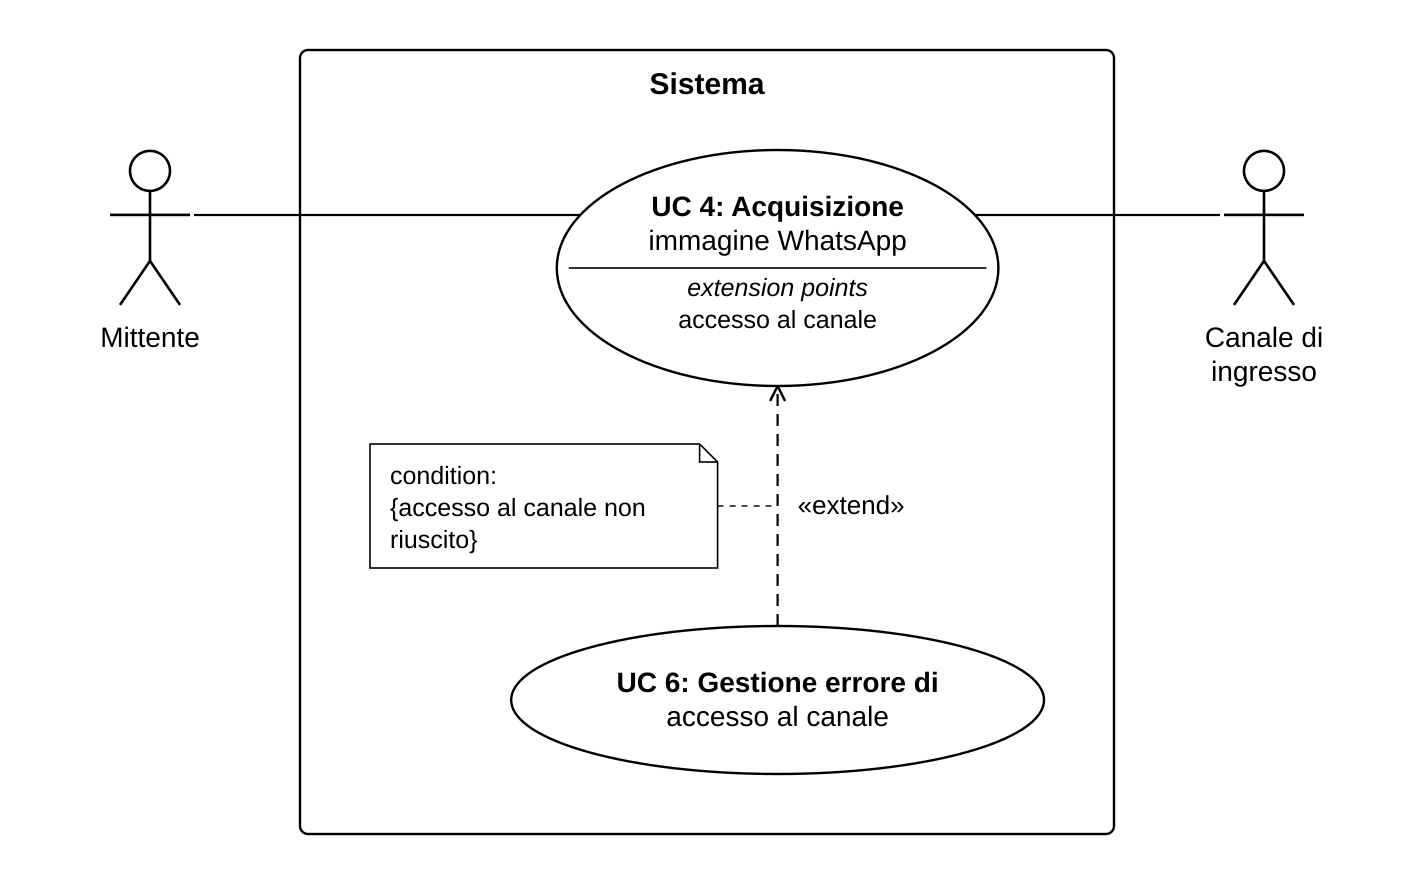
\includegraphics[width=\linewidth,height=0.32\textheight,keepaspectratio]{img/UC4.png}
\caption{UC 4 -- Acquisizione immagine WhatsApp}
\end{center}
\begin{itemize}
    \item \textbf{Attore principale}: Mittente
    \item \textbf{Attori secondari}: Canale di ingresso
    \item \textbf{Precondizioni}: Il canale WhatsApp è configurato e attivo e il sistema è in esecuzione.
    \item \textbf{Scenario principale}:
    \begin{enumerate}
        \item Il mittente invia un'immagine al canale WhatsApp monitorato.
        \item Il sistema rileva il nuovo messaggio.
        \item Il sistema acquisisce il numero del mittente e l'immagine.
        \item Il sistema crea una richiesta associata al messaggio.
    \end{enumerate}
    \item \textbf{Postcondizioni}: La richiesta è acquisita con l'immagine ed è pronta per l'estrazione del testo.
    \item \textbf{Trigger}: Arrivo di un'immagine sul canale WhatsApp.
    \item \textbf{Estensioni}:
    \begin{itemize}
        \item \hyperref[uc:6]{UC 6}: Gestione errore di accesso al canale $\rightarrow$ Condizione: Accesso al canale non riuscito.
    \end{itemize}
\end{itemize}

\subsubsection{UC 5: Acquisizione file da cartella del filesystem}\label{uc:5}
\begin{center}
\captionsetup{type=figure}
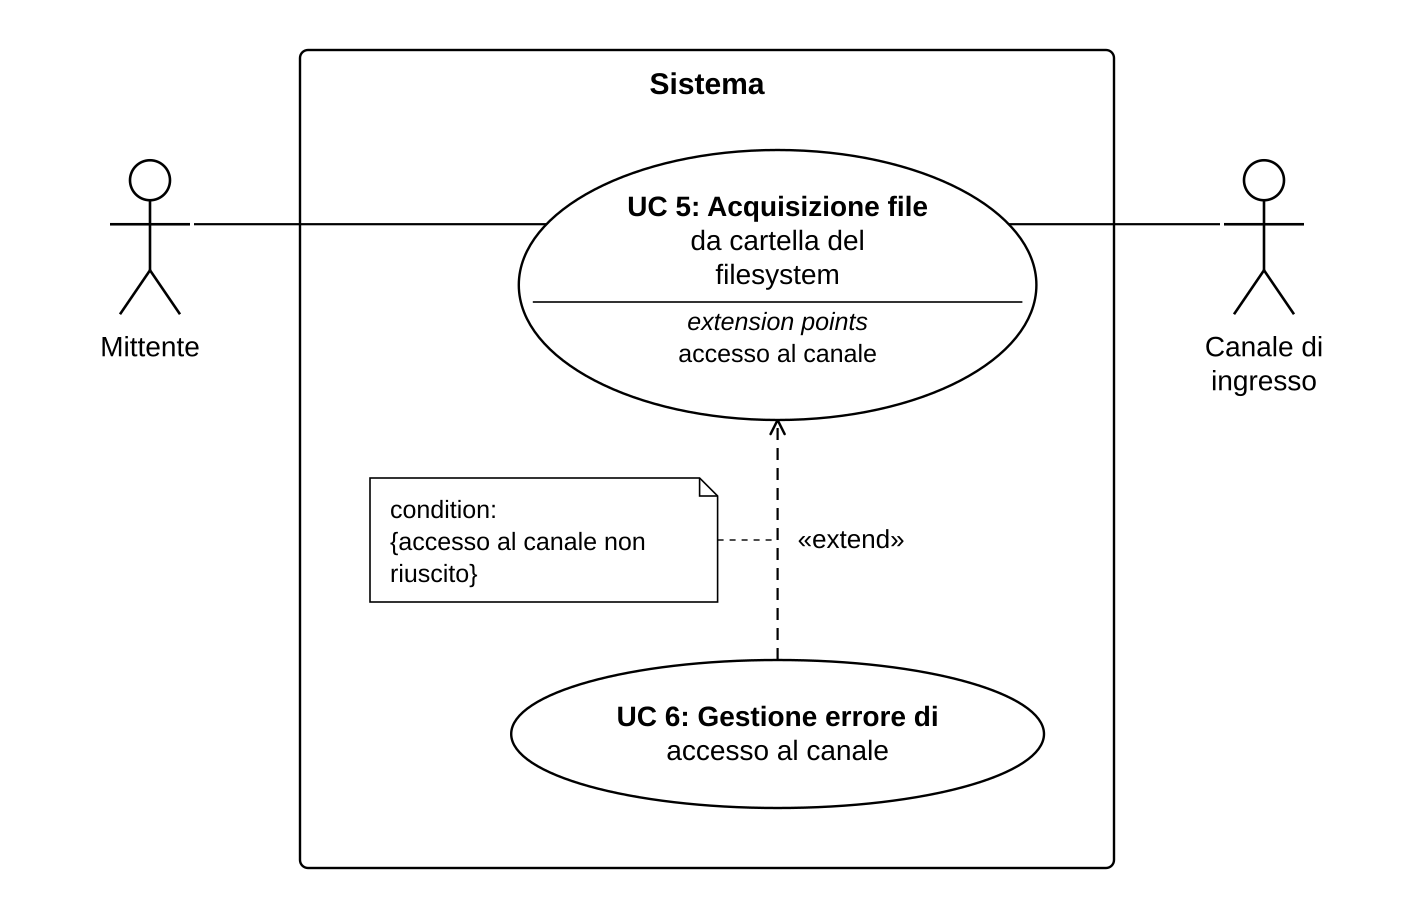
\includegraphics[width=\linewidth,height=0.32\textheight,keepaspectratio]{img/UC5.png}
\caption{UC 5 -- Acquisizione file da cartella del filesystem}
\end{center}
\begin{itemize}
    \item \textbf{Attore principale}: Mittente
    \item \textbf{Attori secondari}: Canale di ingresso
    \item \textbf{Precondizioni}: La cartella del filesystem, locale o remota, è configurata come canale ed è attiva.
    \item \textbf{Scenario principale}:
    \begin{enumerate}
        \item Un nuovo file viene depositato nella cartella monitorata.
        \item Il sistema rileva il nuovo file.
        \item Il sistema acquisisce il file.
        \item Il sistema crea una richiesta associata al file.
    \end{enumerate}
    \item \textbf{Postcondizioni}: La richiesta è acquisita ed è pronta per le fasi successive della pipeline.
    \item \textbf{Trigger}: Deposito di un nuovo file nella cartella monitorata.
    \item \textbf{Estensioni}:
    \begin{itemize}
        \item \hyperref[uc:6]{UC 6}: Gestione errore di accesso al canale $\rightarrow$ Condizione: Accesso al canale non riuscito.
    \end{itemize}
\end{itemize}

\subsubsection{UC 6: Gestione errore di accesso al canale}\label{uc:6}
\begin{center}
\captionsetup{type=figure}
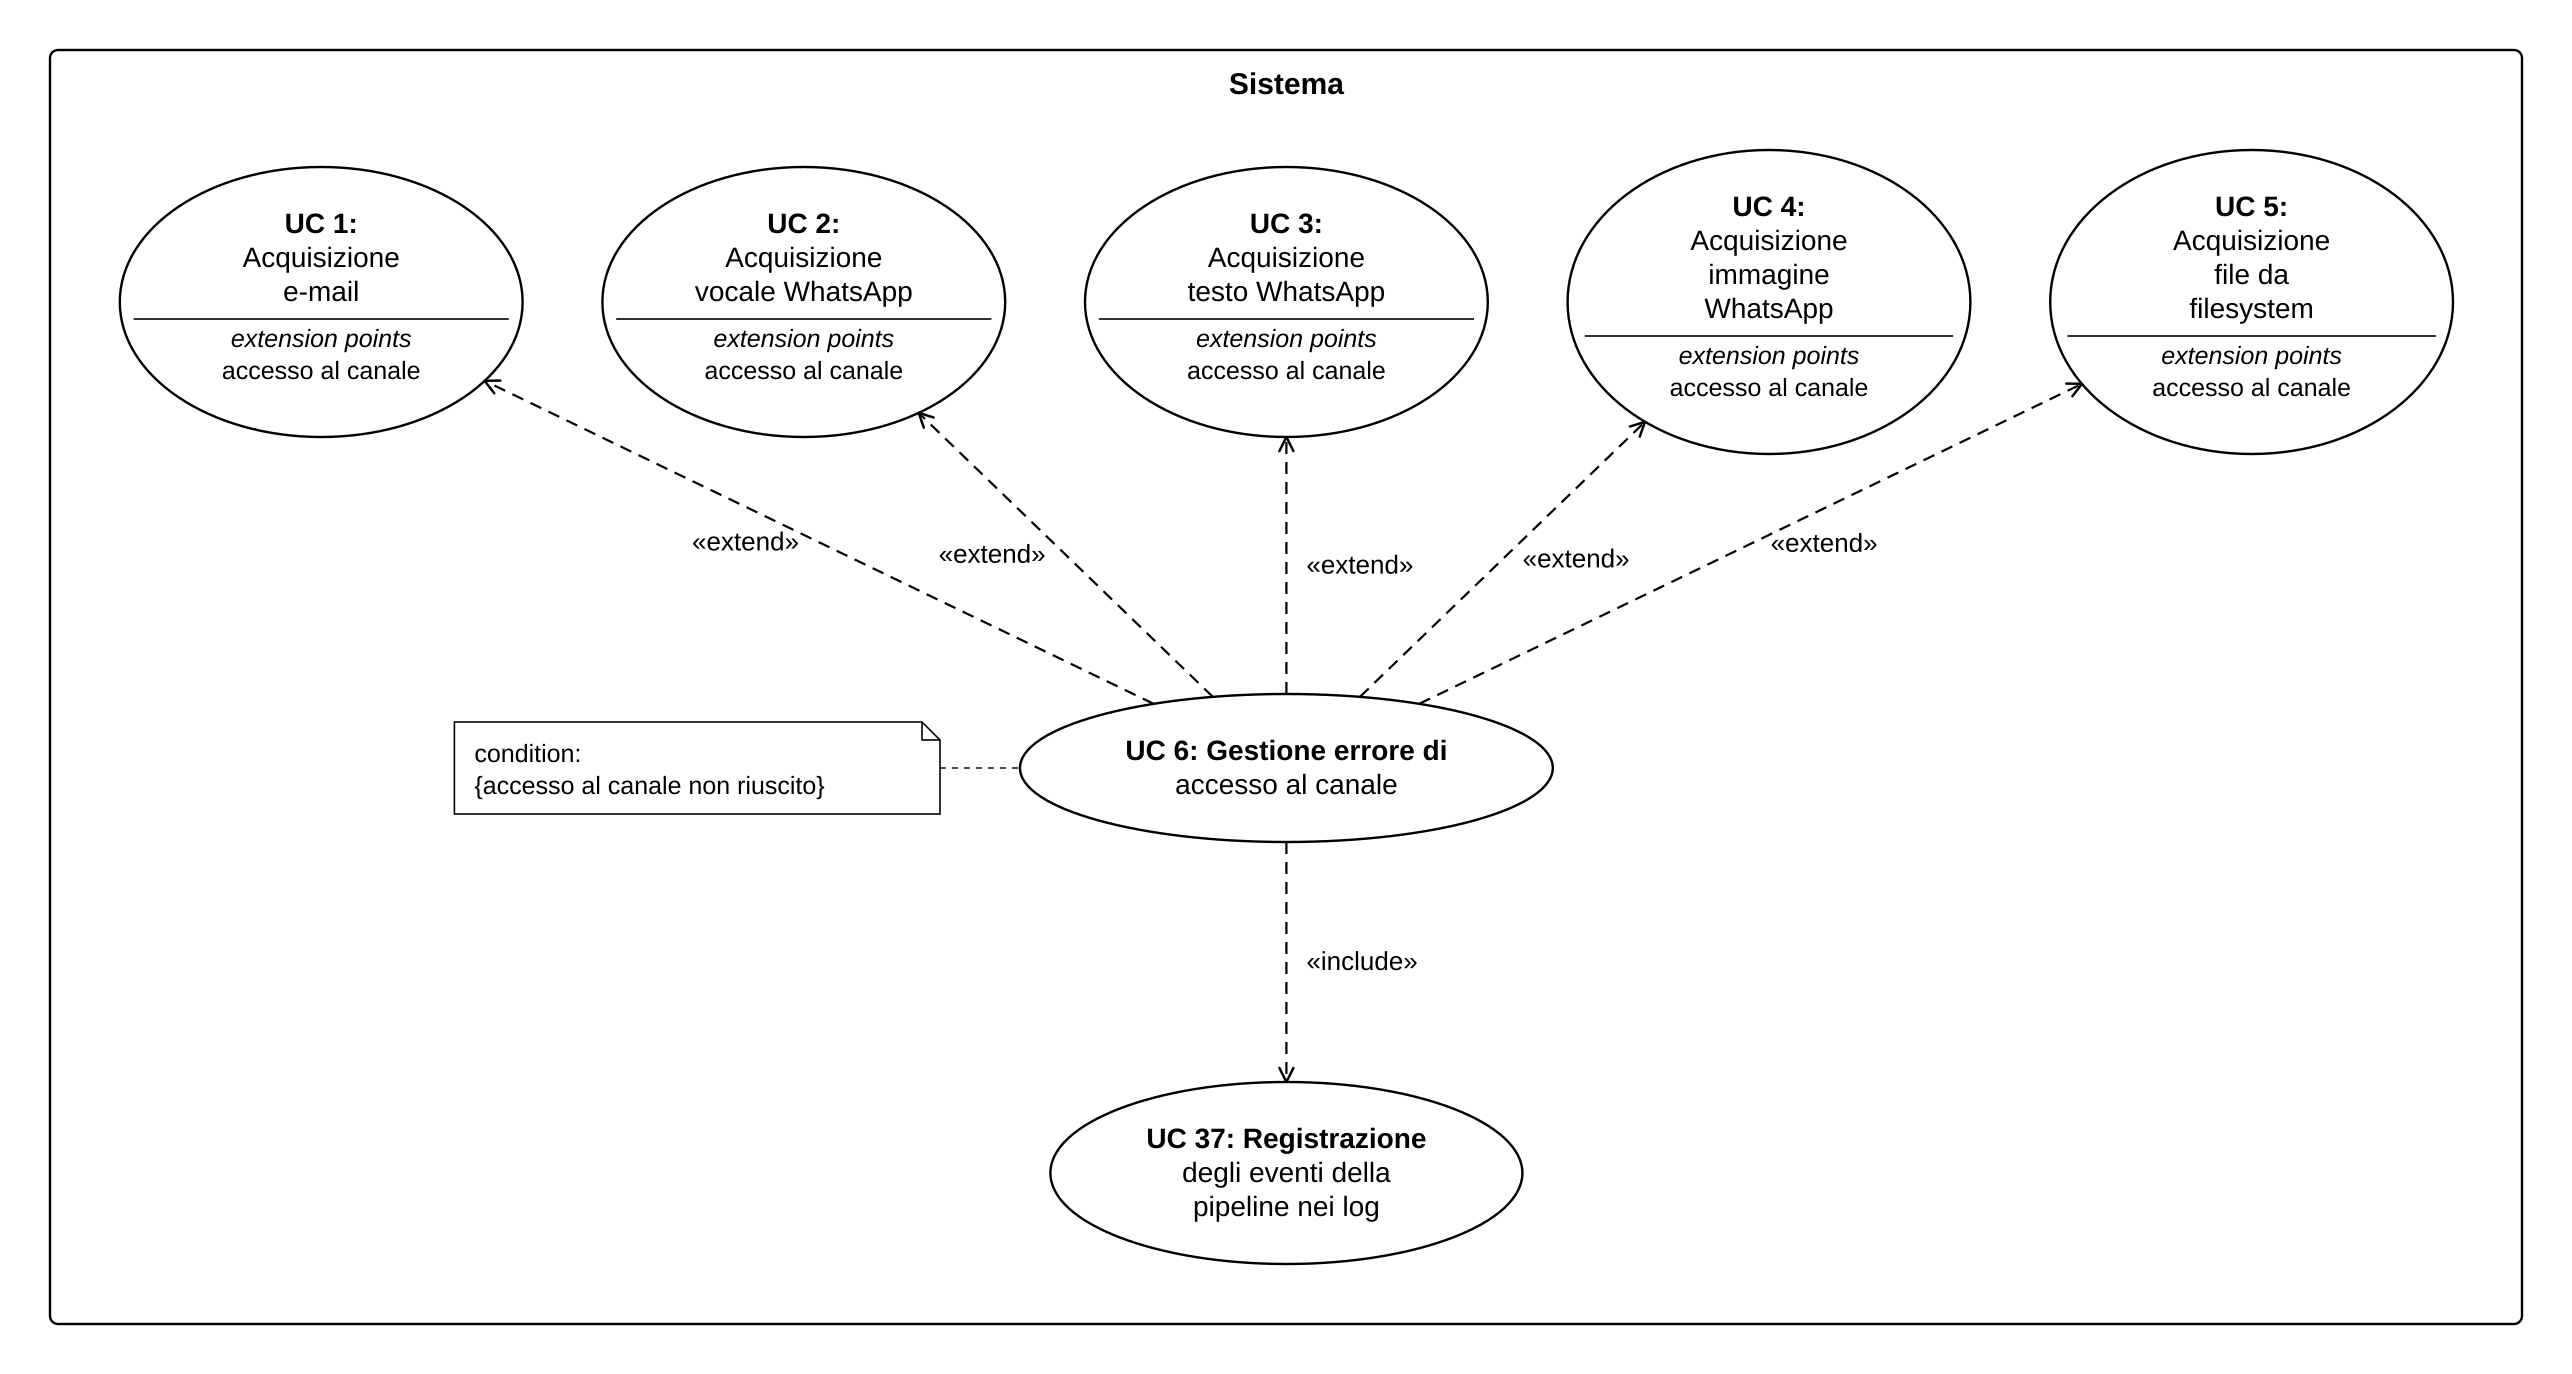
\includegraphics[width=\linewidth,height=0.32\textheight,keepaspectratio]{img/UC6.png}
\caption{UC 6 -- Gestione errore di accesso al canale}
\end{center}
\begin{itemize}
    \item \textbf{Attore principale}: Mittente
    \item \textbf{Precondizioni}: Il monitoraggio di un canale di ingresso è in corso.
    \item \textbf{Scenario principale}:
    \begin{enumerate}
        \item Il sistema rileva un errore di accesso al canale.
        \item Il sistema registra l'errore nei log (\hyperref[uc:37]{UC 37}).
        \item Il sistema riprende il monitoraggio al ciclo successivo.
        \item Il sistema conserva le richieste già acquisite.
    \end{enumerate}
    \item \textbf{Postcondizioni}: L'errore è registrato e nessuna richiesta già acquisita è andata persa.
    \item \textbf{Trigger}: Accesso al canale di ingresso non riuscito.
    \item \textbf{Estende}: \hyperref[uc:1]{UC 1}, \hyperref[uc:2]{UC 2}, \hyperref[uc:3]{UC 3}, \hyperref[uc:4]{UC 4}, \hyperref[uc:5]{UC 5}.
    \item \textbf{Inclusioni}:
    \begin{itemize}
        \item \hyperref[uc:37]{UC 37}: Registrazione degli eventi della pipeline nei log
    \end{itemize}
\end{itemize}

% ------------------------------------------------------------
% MACROAREA 2 --- FILTRO DI SICUREZZA IN INGRESSO
% ------------------------------------------------------------
\subsection{Macroarea 2 --- Filtro di sicurezza in ingresso}

\subsubsection{UC 7: Identificazione del mittente}\label{uc:7}
\begin{center}
\captionsetup{type=figure}
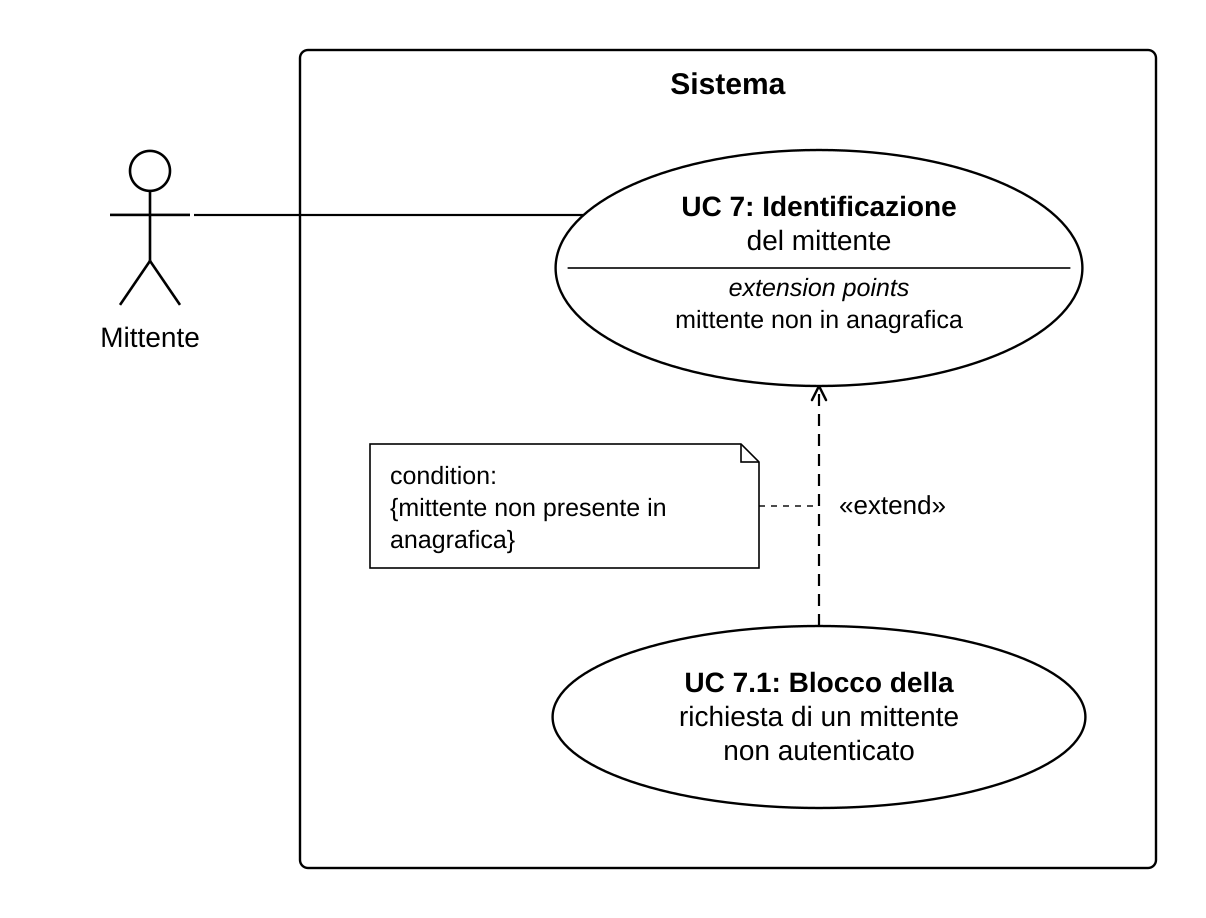
\includegraphics[width=\linewidth,height=0.32\textheight,keepaspectratio]{img/UC7.png}
\caption{UC 7 -- Identificazione del mittente}
\end{center}
\begin{itemize}
    \item \textbf{Attore principale}: Mittente
    \item \textbf{Precondizioni}: Una richiesta è stata acquisita e l'anagrafica clienti è disponibile.
    \item \textbf{Scenario principale}:
    \begin{enumerate}
        \item Il sistema ricava dalla richiesta l'indirizzo e-mail o il numero di telefono del mittente.
        \item Il sistema confronta l'identificativo con l'anagrafica clienti.
        \item Il sistema individua il cliente corrispondente e lo associa alla richiesta.
    \end{enumerate}
    \item \textbf{Postcondizioni}: Il mittente è identificato e associato alla richiesta.
    \item \textbf{Trigger}: Acquisizione di una nuova richiesta.
    \item \textbf{Estensioni}:
    \begin{itemize}
        \item \hyperref[uc:7.1]{UC 7.1}: Blocco della richiesta di un mittente non autenticato $\rightarrow$ Condizione: Mittente non presente in anagrafica.
    \end{itemize}
\end{itemize}

\subsubsection{UC 7.1: Blocco della richiesta di un mittente non autenticato}\label{uc:7.1}
\begin{center}
\captionsetup{type=figure}
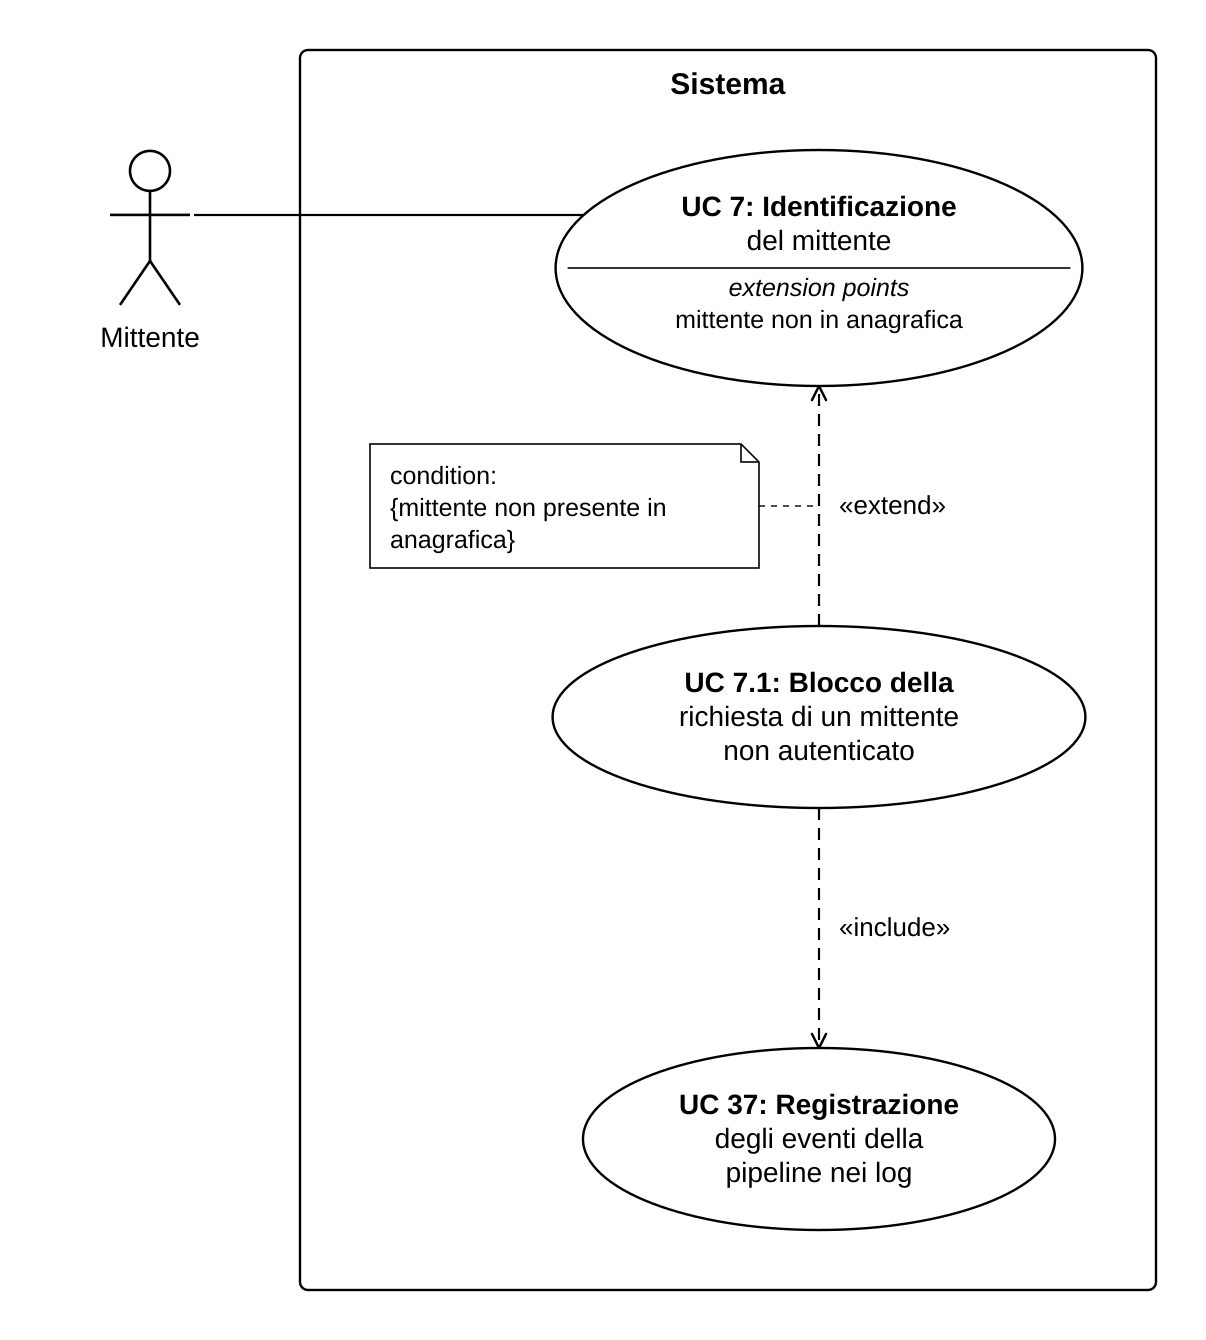
\includegraphics[width=\linewidth,height=0.32\textheight,keepaspectratio]{img/UC7_1.png}
\caption{UC 7.1 -- Blocco della richiesta di un mittente non autenticato}
\end{center}
\begin{itemize}
    \item \textbf{Attore principale}: Mittente
    \item \textbf{Precondizioni}: L'identificazione del mittente è in corso.
    \item \textbf{Scenario principale}:
    \begin{enumerate}
        \item Il sistema non trova il mittente in anagrafica.
        \item Il sistema blocca la richiesta.
        \item Il sistema registra l'evento nei log (\hyperref[uc:37]{UC 37}).
    \end{enumerate}
    \item \textbf{Postcondizioni}: La richiesta è bloccata e non viene elaborata; l'evento è registrato nei log.
    \item \textbf{Trigger}: Mittente non presente in anagrafica.
    \item \textbf{Estende}: \hyperref[uc:7]{UC 7}.
    \item \textbf{Inclusioni}:
    \begin{itemize}
        \item \hyperref[uc:37]{UC 37}: Registrazione degli eventi della pipeline nei log
    \end{itemize}
\end{itemize}

\subsubsection{UC 8: Verifica dell'autorizzazione del tenant}\label{uc:8}
\begin{center}
\captionsetup{type=figure}
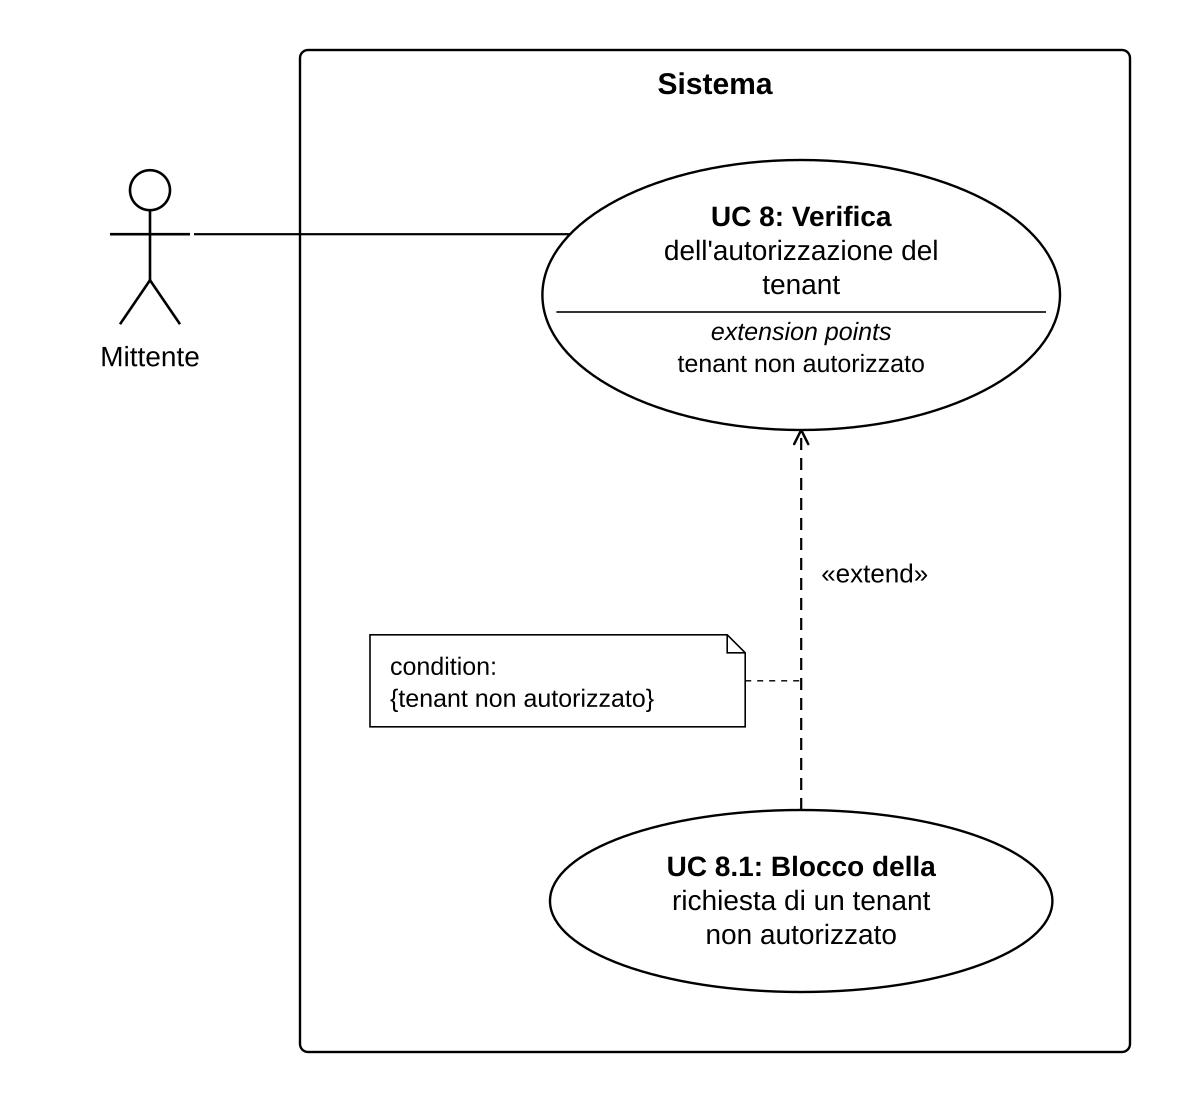
\includegraphics[width=\linewidth,height=0.32\textheight,keepaspectratio]{img/UC8.png}
\caption{UC 8 -- Verifica dell'autorizzazione del tenant}
\end{center}
\begin{itemize}
    \item \textbf{Attore principale}: Mittente
    \item \textbf{Precondizioni}: Il mittente è stato identificato.
    \item \textbf{Scenario principale}:
    \begin{enumerate}
        \item Il sistema determina il tenant del mittente.
        \item Il sistema verifica che il tenant sia autorizzato.
        \item Il sistema consente l'elaborazione della richiesta.
    \end{enumerate}
    \item \textbf{Postcondizioni}: Il tenant è verificato e la richiesta può proseguire.
    \item \textbf{Trigger}: Identificazione del mittente completata.
    \item \textbf{Estensioni}:
    \begin{itemize}
        \item \hyperref[uc:8.1]{UC 8.1}: Blocco della richiesta di un tenant non autorizzato $\rightarrow$ Condizione: Tenant non autorizzato.
    \end{itemize}
\end{itemize}

\subsubsection{UC 8.1: Blocco della richiesta di un tenant non autorizzato}\label{uc:8.1}
\begin{center}
\captionsetup{type=figure}
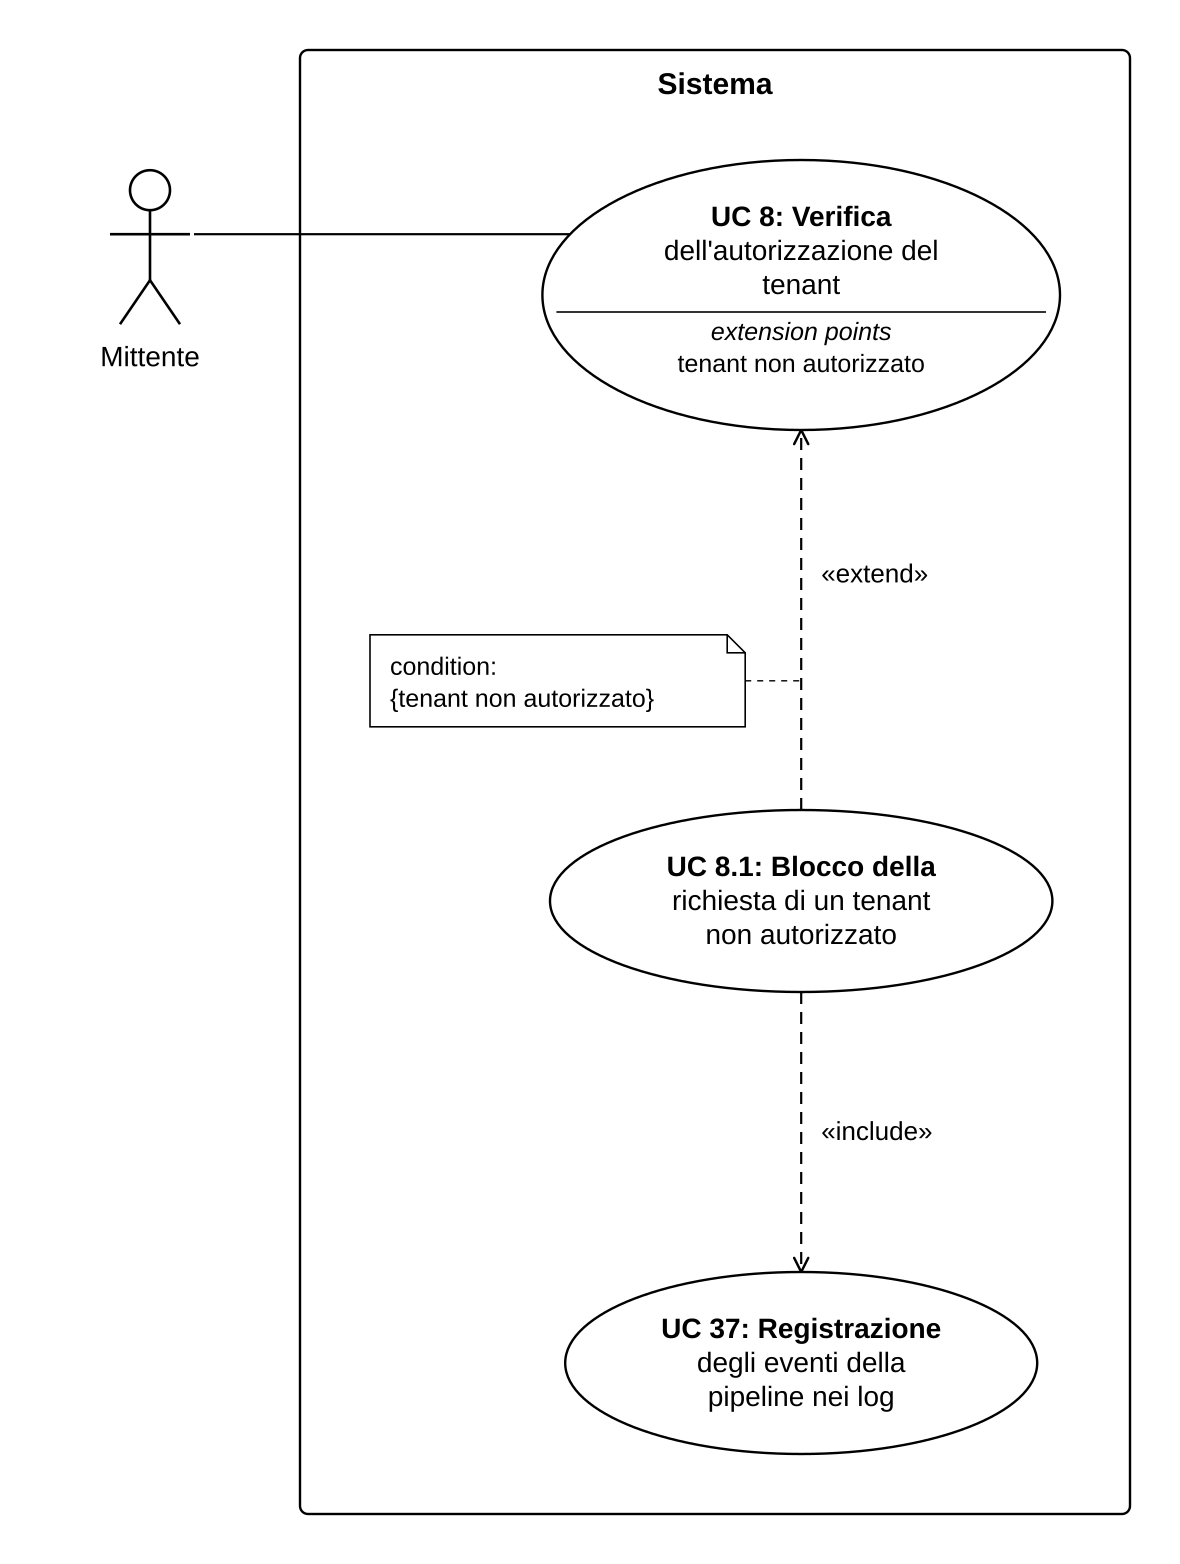
\includegraphics[width=\linewidth,height=0.32\textheight,keepaspectratio]{img/UC8_1.png}
\caption{UC 8.1 -- Blocco della richiesta di un tenant non autorizzato}
\end{center}
\begin{itemize}
    \item \textbf{Attore principale}: Mittente
    \item \textbf{Precondizioni}: La verifica del tenant è in corso.
    \item \textbf{Scenario principale}:
    \begin{enumerate}
        \item Il sistema rileva che il tenant non è autorizzato.
        \item Il sistema blocca la richiesta.
        \item Il sistema registra l'evento nei log (\hyperref[uc:37]{UC 37}).
    \end{enumerate}
    \item \textbf{Postcondizioni}: La richiesta è bloccata e non viene elaborata; l'evento è registrato nei log.
    \item \textbf{Trigger}: Tenant del mittente non autorizzato.
    \item \textbf{Estende}: \hyperref[uc:8]{UC 8}.
    \item \textbf{Inclusioni}:
    \begin{itemize}
        \item \hyperref[uc:37]{UC 37}: Registrazione degli eventi della pipeline nei log
    \end{itemize}
\end{itemize}

\subsubsection{UC 9: Controllo anti-spam delle e-mail}\label{uc:9}
\begin{center}
\captionsetup{type=figure}
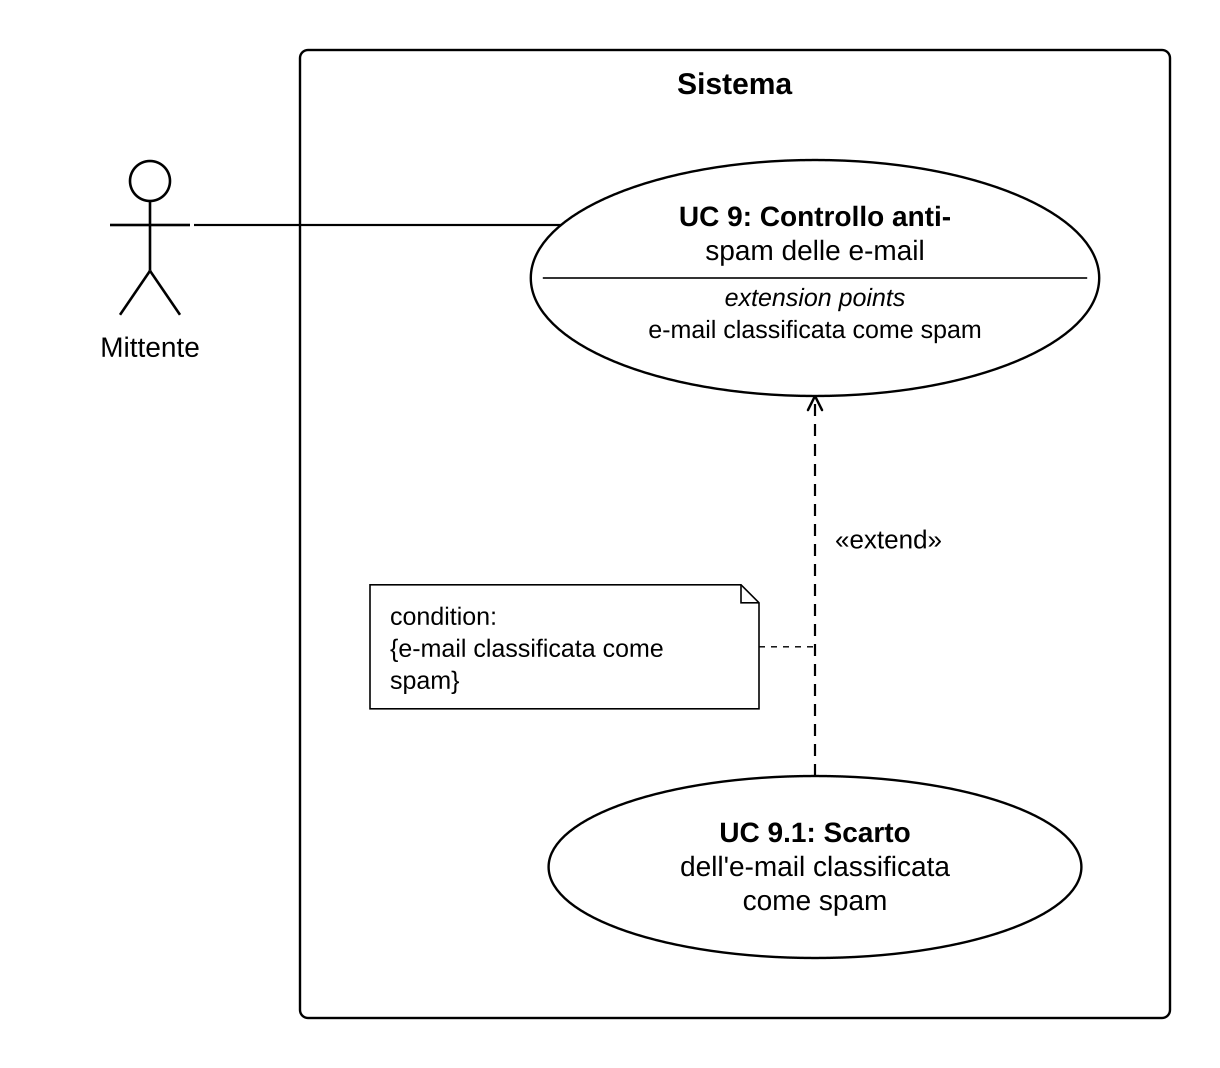
\includegraphics[width=\linewidth,height=0.32\textheight,keepaspectratio]{img/UC9.png}
\caption{UC 9 -- Controllo anti-spam delle e-mail}
\end{center}
\begin{itemize}
    \item \textbf{Attore principale}: Mittente
    \item \textbf{Precondizioni}: Una richiesta proveniente da un'e-mail è stata acquisita.
    \item \textbf{Scenario principale}:
    \begin{enumerate}
        \item Il sistema applica il controllo anti-spam al messaggio.
        \item Il sistema classifica il messaggio come non spam.
        \item Il sistema consente la prosecuzione dell'elaborazione.
    \end{enumerate}
    \item \textbf{Postcondizioni}: L'e-mail è classificata come non spam e la richiesta prosegue.
    \item \textbf{Trigger}: Acquisizione di una richiesta da e-mail.
    \item \textbf{Estensioni}:
    \begin{itemize}
        \item \hyperref[uc:9.1]{UC 9.1}: Scarto dell'e-mail classificata come spam $\rightarrow$ Condizione: E-mail classificata come spam.
    \end{itemize}
\end{itemize}

\subsubsection{UC 9.1: Scarto dell'e-mail classificata come spam}\label{uc:9.1}
\begin{center}
\captionsetup{type=figure}
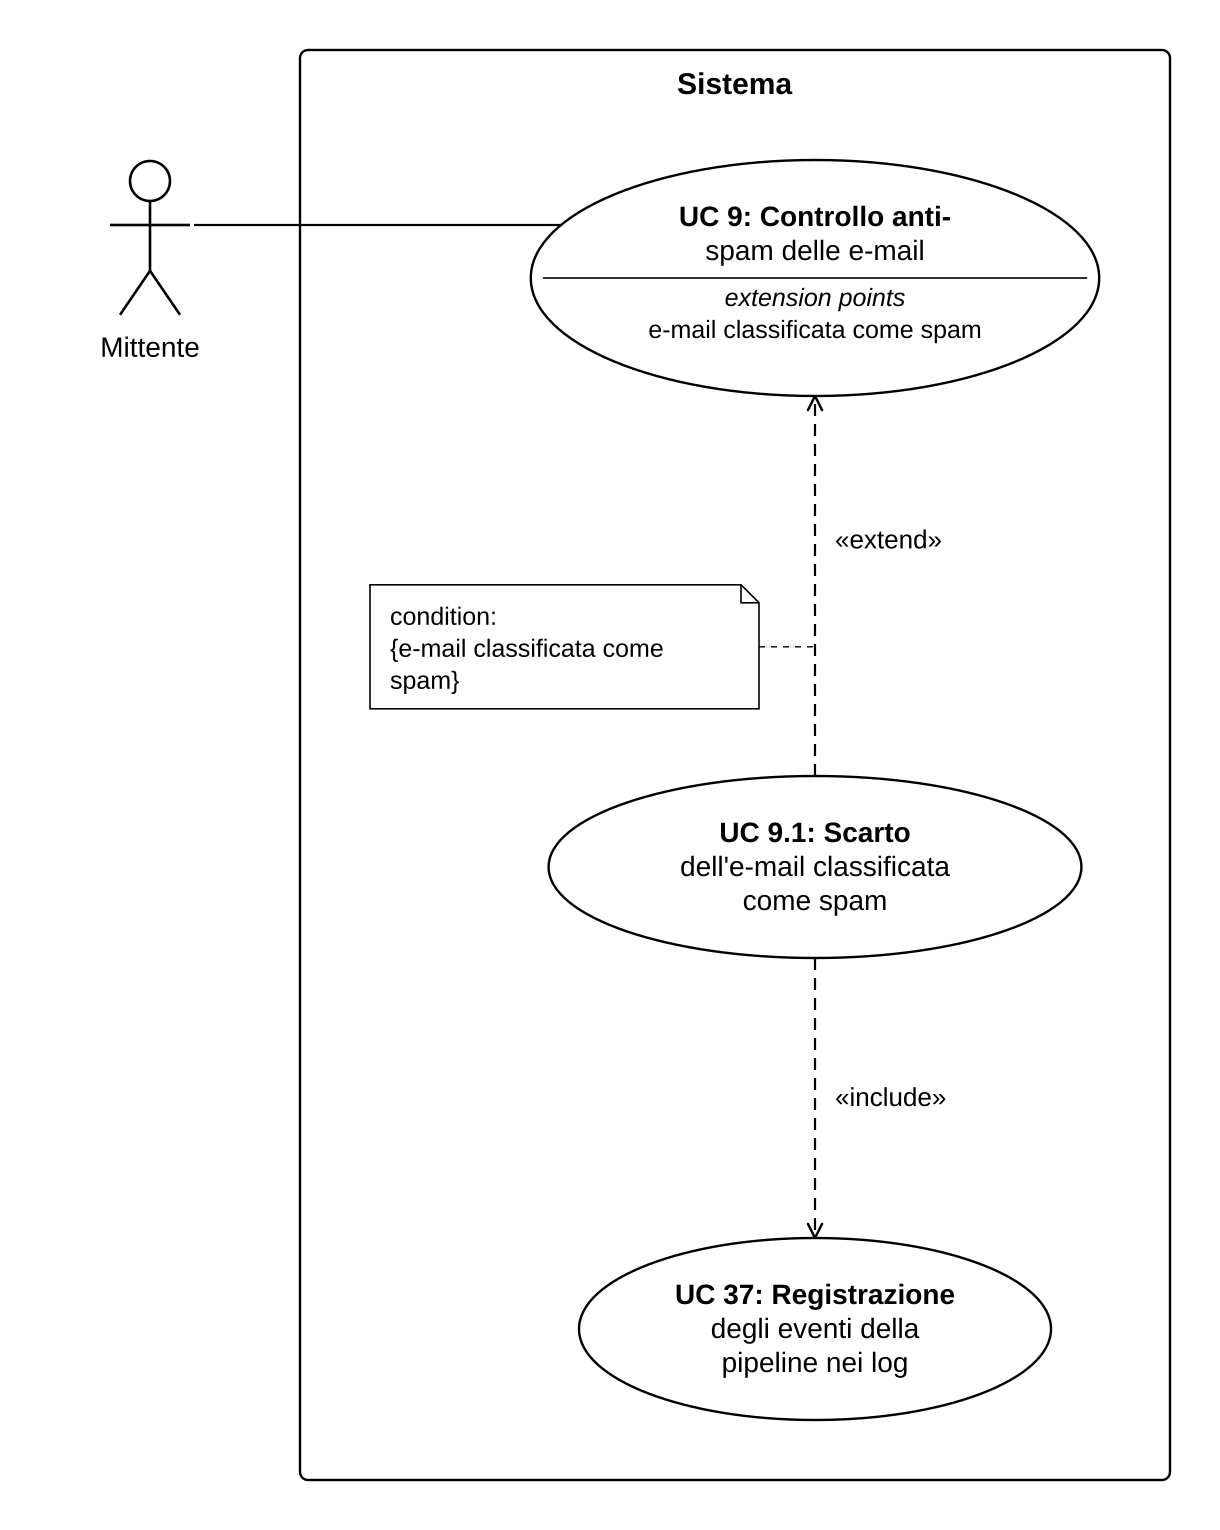
\includegraphics[width=\linewidth,height=0.32\textheight,keepaspectratio]{img/UC9_1.png}
\caption{UC 9.1 -- Scarto dell'e-mail classificata come spam}
\end{center}
\begin{itemize}
    \item \textbf{Attore principale}: Mittente
    \item \textbf{Precondizioni}: Il controllo anti-spam è in corso.
    \item \textbf{Scenario principale}:
    \begin{enumerate}
        \item Il sistema classifica l'e-mail come spam.
        \item Il sistema scarta la richiesta.
        \item Il sistema registra l'evento nei log (\hyperref[uc:37]{UC 37}).
    \end{enumerate}
    \item \textbf{Postcondizioni}: La richiesta è scartata e l'evento è registrato nei log.
    \item \textbf{Trigger}: E-mail classificata come spam.
    \item \textbf{Estende}: \hyperref[uc:9]{UC 9}.
    \item \textbf{Inclusioni}:
    \begin{itemize}
        \item \hyperref[uc:37]{UC 37}: Registrazione degli eventi della pipeline nei log
    \end{itemize}
\end{itemize}

\subsubsection{UC 10: Rilevamento delle richieste duplicate}\label{uc:10}
\begin{center}
\captionsetup{type=figure}
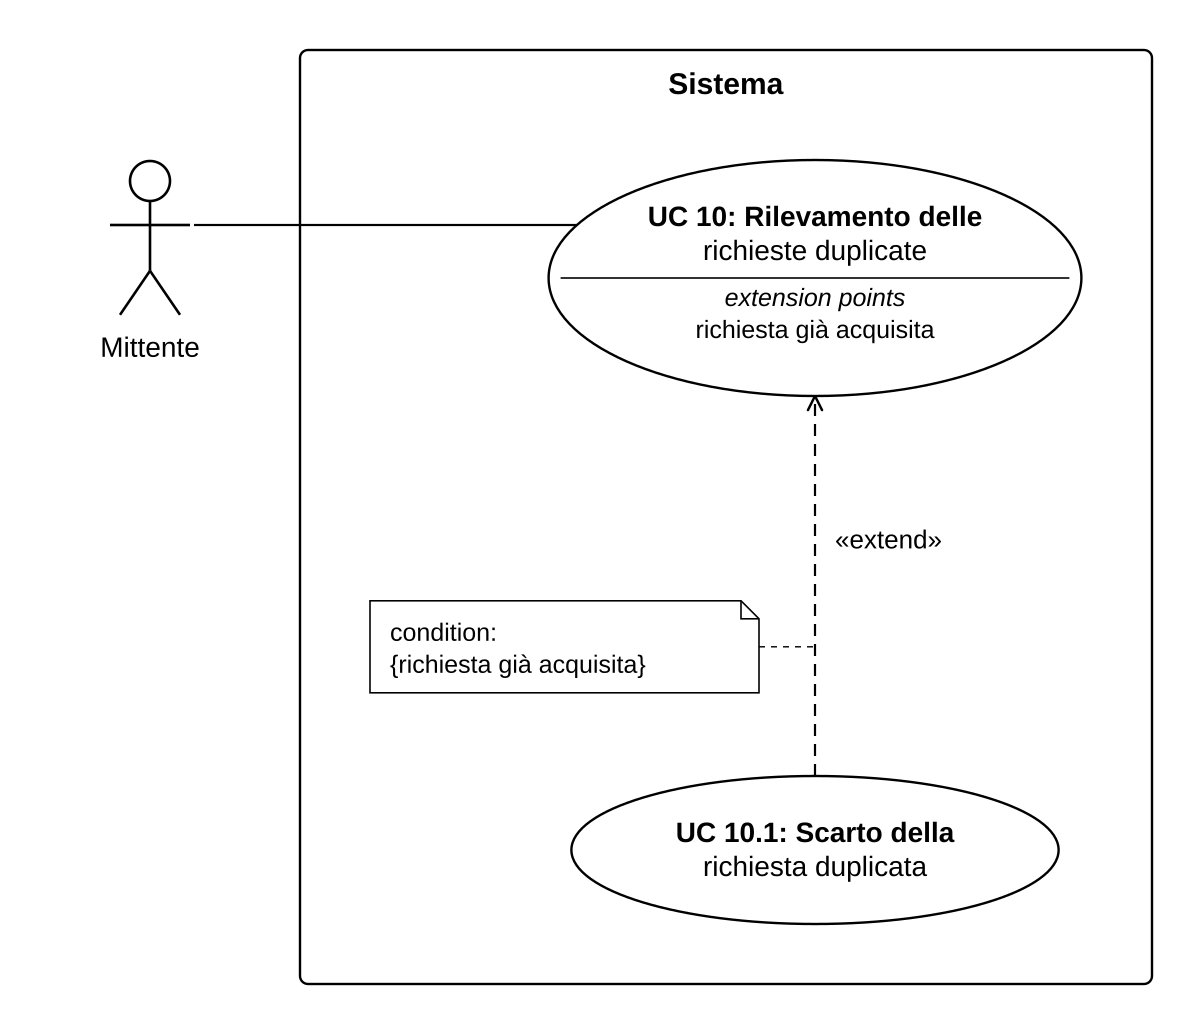
\includegraphics[width=\linewidth,height=0.32\textheight,keepaspectratio]{img/UC10.png}
\caption{UC 10 -- Rilevamento delle richieste duplicate}
\end{center}
\begin{itemize}
    \item \textbf{Attore principale}: Mittente
    \item \textbf{Precondizioni}: Una richiesta è stata acquisita.
    \item \textbf{Scenario principale}:
    \begin{enumerate}
        \item Il sistema confronta la richiesta con quelle già acquisite.
        \item Il sistema stabilisce che la richiesta non è un duplicato.
        \item Il sistema consente la prosecuzione dell'elaborazione.
    \end{enumerate}
    \item \textbf{Postcondizioni}: La richiesta è riconosciuta come nuova e prosegue.
    \item \textbf{Trigger}: Acquisizione di una richiesta.
    \item \textbf{Estensioni}:
    \begin{itemize}
        \item \hyperref[uc:10.1]{UC 10.1}: Scarto della richiesta duplicata $\rightarrow$ Condizione: Richiesta già acquisita.
    \end{itemize}
\end{itemize}

\subsubsection{UC 10.1: Scarto della richiesta duplicata}\label{uc:10.1}
\begin{center}
\captionsetup{type=figure}
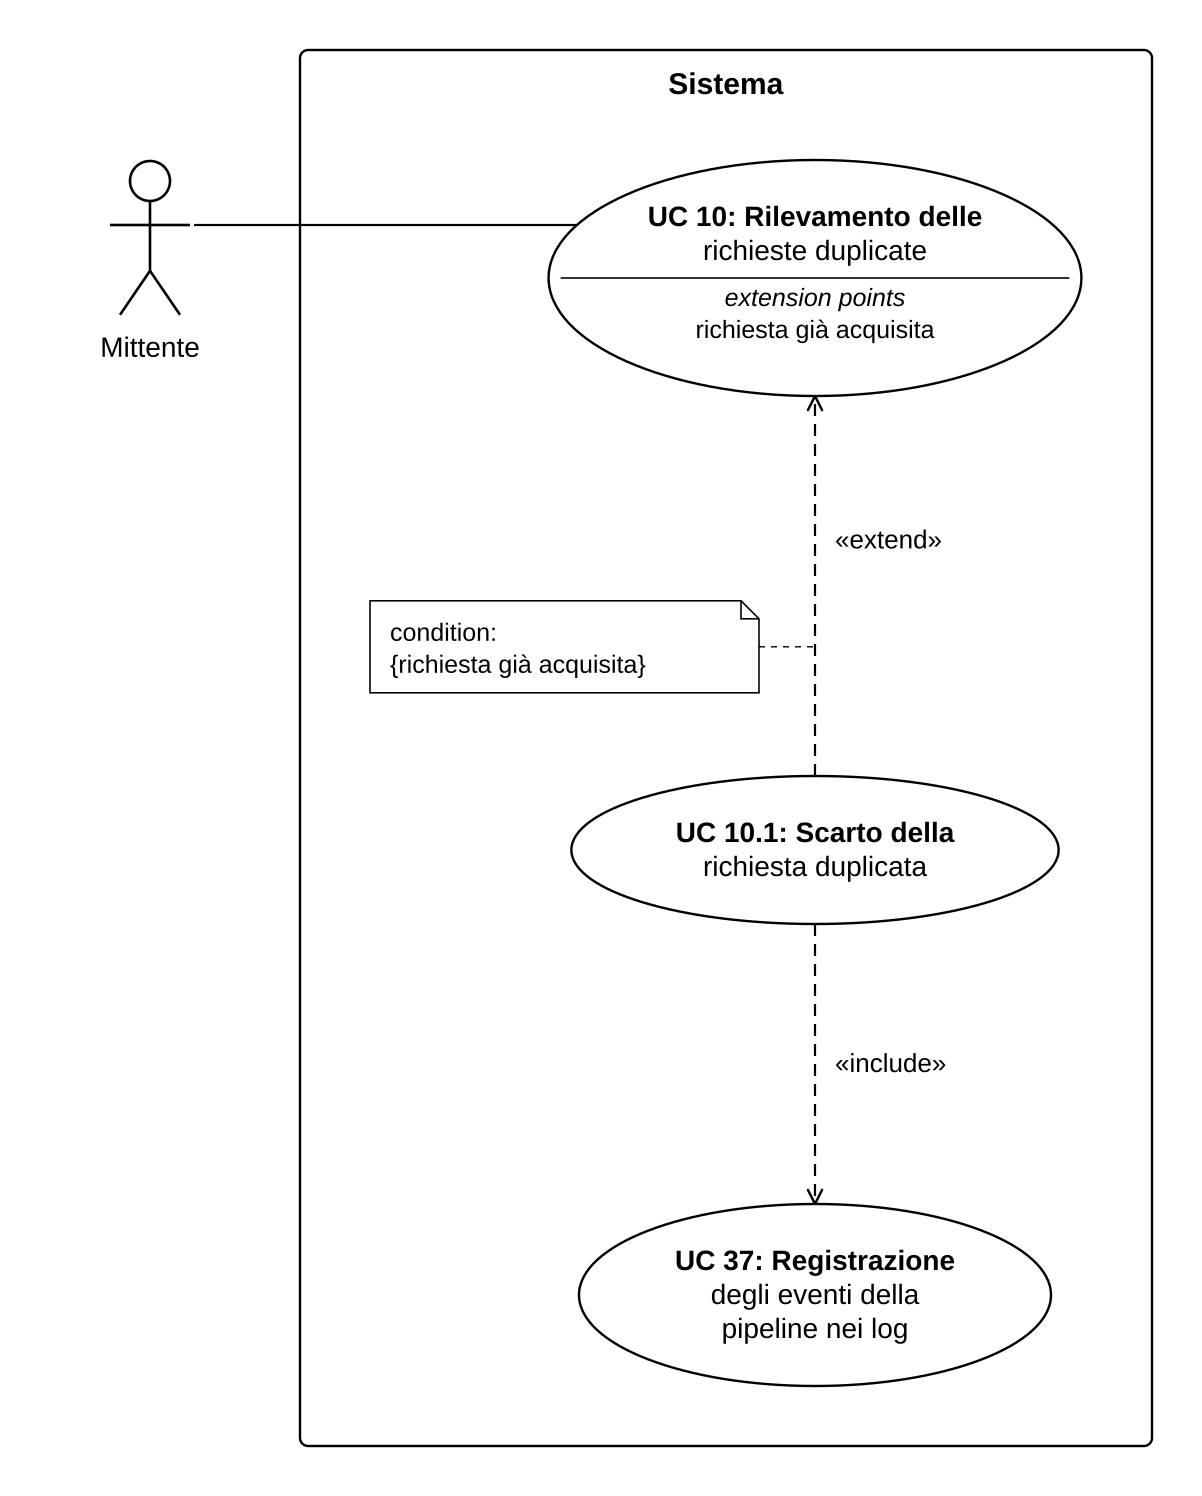
\includegraphics[width=\linewidth,height=0.32\textheight,keepaspectratio]{img/UC10_1.png}
\caption{UC 10.1 -- Scarto della richiesta duplicata}
\end{center}
\begin{itemize}
    \item \textbf{Attore principale}: Mittente
    \item \textbf{Precondizioni}: Il rilevamento dei duplicati è in corso.
    \item \textbf{Scenario principale}:
    \begin{enumerate}
        \item Il sistema rileva che la richiesta è già stata acquisita.
        \item Il sistema scarta la richiesta.
        \item Il sistema registra l'evento nei log (\hyperref[uc:37]{UC 37}).
    \end{enumerate}
    \item \textbf{Postcondizioni}: La richiesta duplicata è scartata e l'evento è registrato nei log.
    \item \textbf{Trigger}: Richiesta già acquisita in precedenza.
    \item \textbf{Estende}: \hyperref[uc:10]{UC 10}.
    \item \textbf{Inclusioni}:
    \begin{itemize}
        \item \hyperref[uc:37]{UC 37}: Registrazione degli eventi della pipeline nei log
    \end{itemize}
\end{itemize}

\subsubsection{UC 11: Anonimizzazione delle informazioni private}\label{uc:11}
\begin{center}
\captionsetup{type=figure}
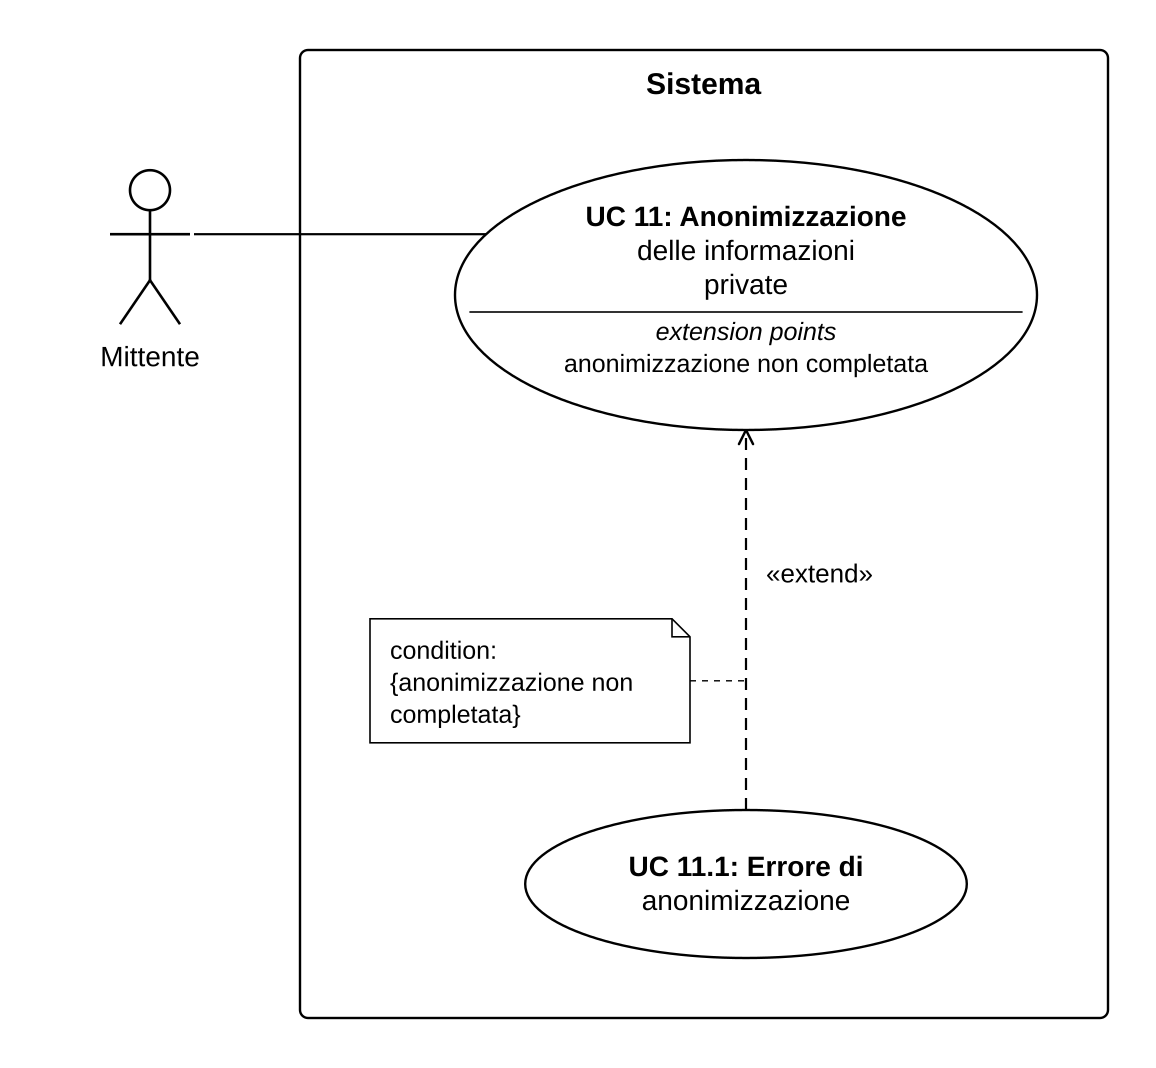
\includegraphics[width=\linewidth,height=0.32\textheight,keepaspectratio]{img/UC11.png}
\caption{UC 11 -- Anonimizzazione delle informazioni private}
\end{center}
\begin{itemize}
    \item \textbf{Attore principale}: Mittente
    \item \textbf{Precondizioni}: La richiesta ha superato i controlli di sicurezza precedenti.
    \item \textbf{Scenario principale}:
    \begin{enumerate}
        \item Il sistema individua le informazioni private presenti nella richiesta.
        \item Il sistema anonimizza le informazioni individuate.
        \item Il sistema consente la prosecuzione dell'elaborazione.
    \end{enumerate}
    \item \textbf{Postcondizioni}: Le informazioni private sono anonimizzate.
    \item \textbf{Trigger}: Prosecuzione della richiesta dopo i controlli di accesso.
    \item \textbf{Estensioni}:
    \begin{itemize}
        \item \hyperref[uc:11.1]{UC 11.1}: Errore di anonimizzazione $\rightarrow$ Condizione: Anonimizzazione non completata.
    \end{itemize}
\end{itemize}

\subsubsection{UC 11.1: Errore di anonimizzazione}\label{uc:11.1}
\begin{center}
\captionsetup{type=figure}
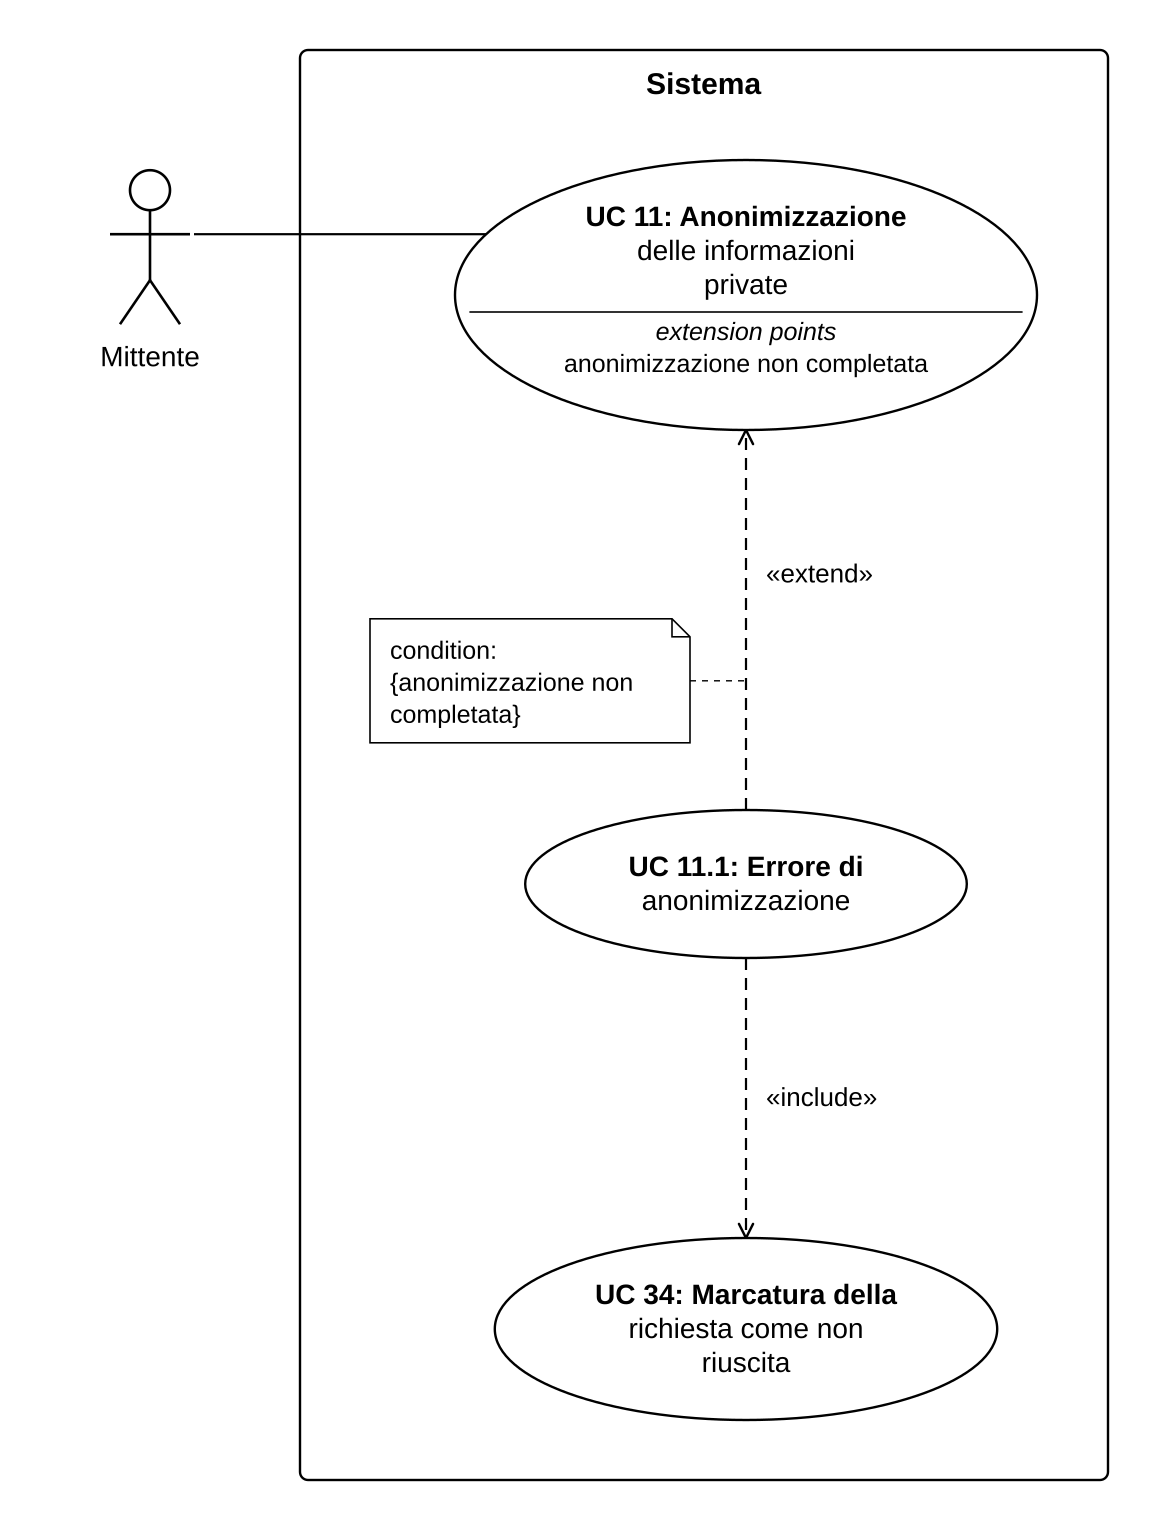
\includegraphics[width=\linewidth,height=0.32\textheight,keepaspectratio]{img/UC11_1.png}
\caption{UC 11.1 -- Errore di anonimizzazione}
\end{center}
\begin{itemize}
    \item \textbf{Attore principale}: Mittente
    \item \textbf{Precondizioni}: L'anonimizzazione è in corso.
    \item \textbf{Scenario principale}:
    \begin{enumerate}
        \item Il sistema rileva che l'anonimizzazione non si completa correttamente.
        \item Il sistema marca la richiesta come non riuscita (\hyperref[uc:34]{UC 34}).
        \item Il sistema registra l'errore nei log (\hyperref[uc:37]{UC 37}).
    \end{enumerate}
    \item \textbf{Postcondizioni}: La richiesta è marcata come non riuscita e l'errore è registrato nei log.
    \item \textbf{Trigger}: Anonimizzazione non completata.
    \item \textbf{Estende}: \hyperref[uc:11]{UC 11}.
    \item \textbf{Inclusioni}:
    \begin{itemize}
        \item \hyperref[uc:34]{UC 34}: Marcatura della richiesta come non riuscita
    \end{itemize}
\end{itemize}

\subsubsection{UC 12: Aggiornamento dell'anagrafica clienti tramite elaborazione batch}\label{uc:12}
\begin{center}
\captionsetup{type=figure}
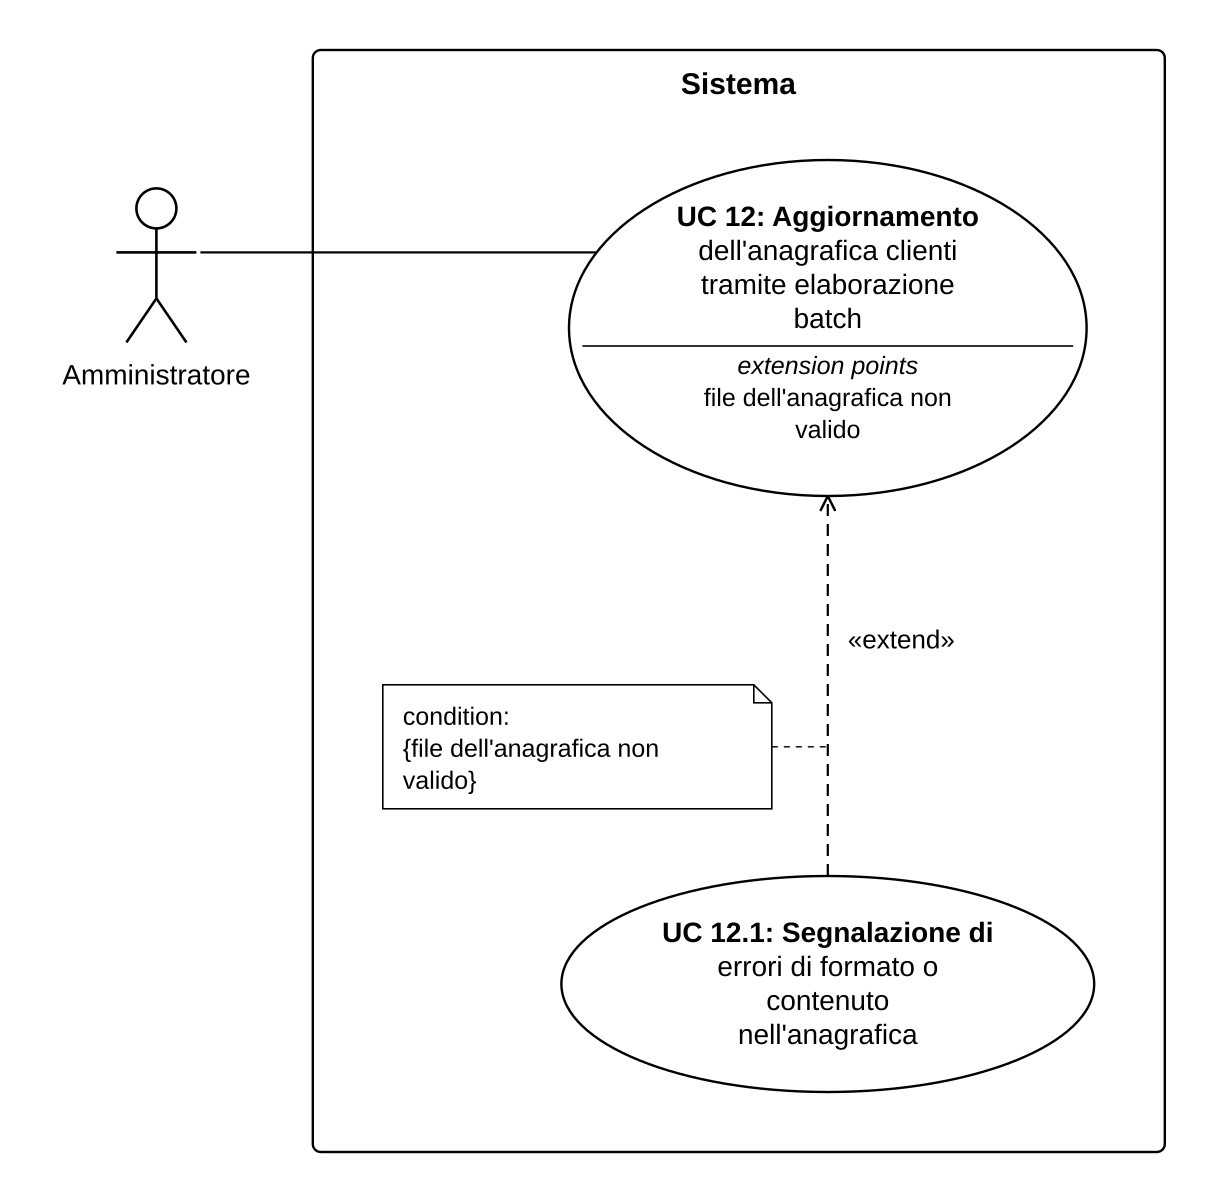
\includegraphics[width=\linewidth,height=0.32\textheight,keepaspectratio]{img/UC12.png}
\caption{UC 12 -- Aggiornamento dell'anagrafica clienti tramite elaborazione batch}
\end{center}
\begin{itemize}
    \item \textbf{Attore principale}: Amministratore
    \item \textbf{Precondizioni}: L'Amministratore è autenticato e i dati dell'anagrafica forniti dall'azienda sono disponibili.
    \item \textbf{Scenario principale}:
    \begin{enumerate}
        \item L'Amministratore avvia l'aggiornamento dell'anagrafica fornendo i dati.
        \item Il sistema verifica formato e contenuto dei dati.
        \item Il sistema elabora i dati in modalità batch e aggiorna l'anagrafica clienti.
        \item Il sistema conferma l'esito dell'aggiornamento.
    \end{enumerate}
    \item \textbf{Postcondizioni}: L'anagrafica clienti è aggiornata.
    \item \textbf{Trigger}: L'Amministratore vuole aggiornare l'anagrafica clienti.
    \item \textbf{Estensioni}:
    \begin{itemize}
        \item \hyperref[uc:12.1]{UC 12.1}: Segnalazione di errori di formato o contenuto nell'anagrafica $\rightarrow$ Condizione: File dell'anagrafica non valido.
    \end{itemize}
\end{itemize}

\subsubsection{UC 12.1: Segnalazione di errori di formato o contenuto nell'anagrafica}\label{uc:12.1}
\begin{center}
\captionsetup{type=figure}
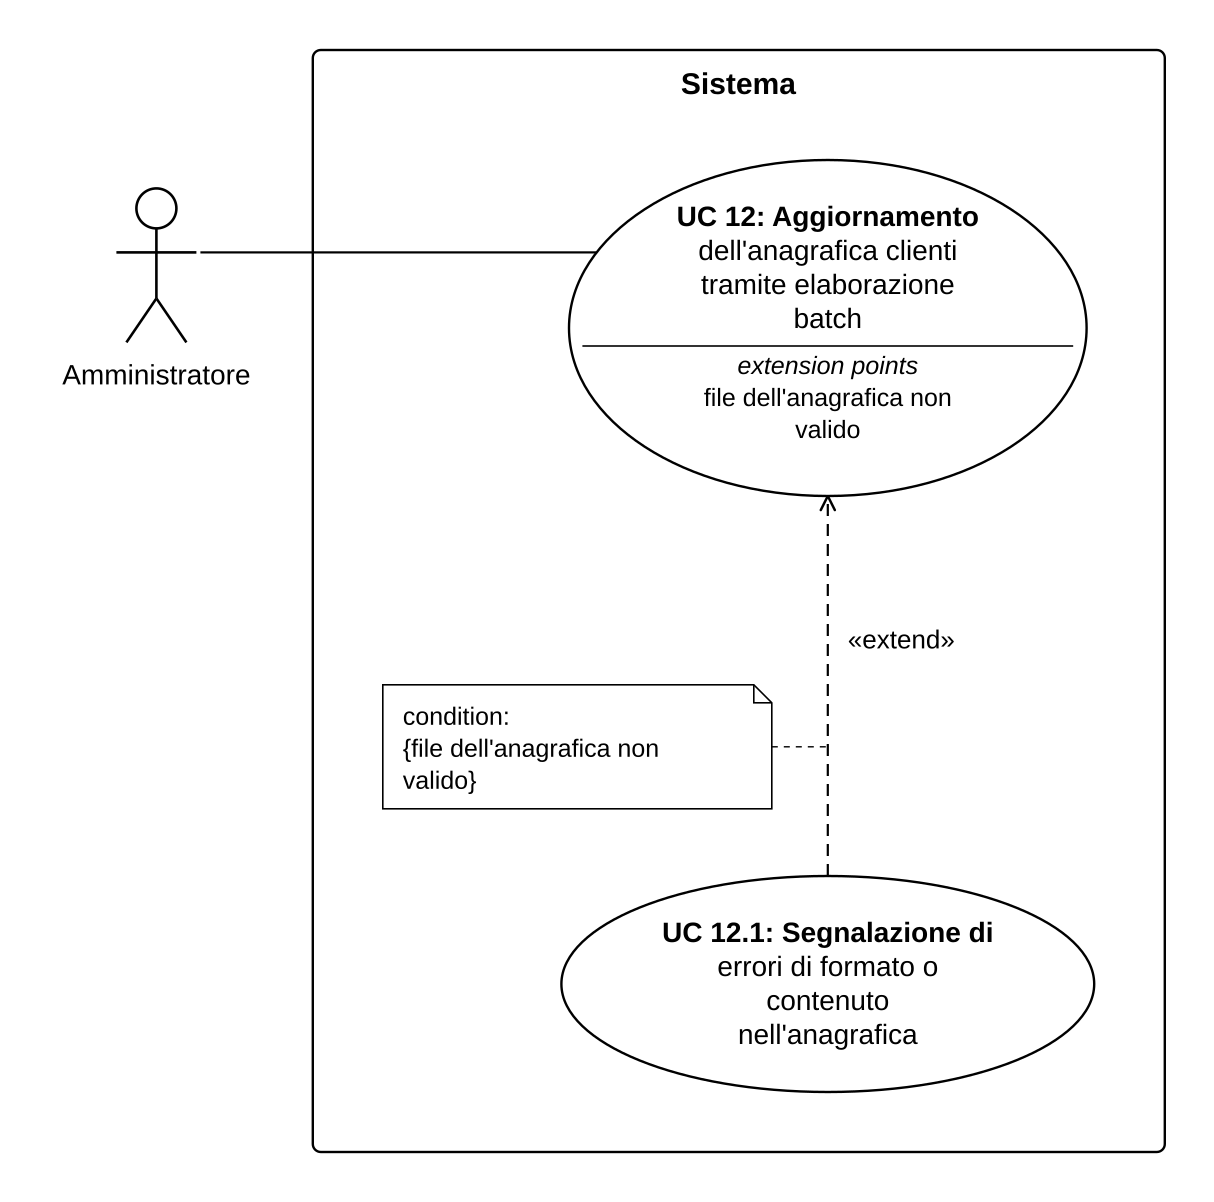
\includegraphics[width=\linewidth,height=0.32\textheight,keepaspectratio]{img/UC12_1.png}
\caption{UC 12.1 -- Segnalazione di errori di formato o contenuto nell'anagrafica}
\end{center}
\begin{itemize}
    \item \textbf{Attore principale}: Amministratore
    \item \textbf{Precondizioni}: L'aggiornamento dell'anagrafica è in corso.
    \item \textbf{Scenario principale}:
    \begin{enumerate}
        \item Il sistema rileva errori di formato o di contenuto nei dati.
        \item Il sistema segnala gli errori all'Amministratore.
        \item Il sistema non modifica l'anagrafica esistente.
    \end{enumerate}
    \item \textbf{Postcondizioni}: L'anagrafica esistente è invariata e gli errori sono stati segnalati.
    \item \textbf{Trigger}: Dati dell'anagrafica non validi.
    \item \textbf{Estende}: \hyperref[uc:12]{UC 12}.
\end{itemize}

\subsubsection{UC 13: Consultazione dell'anagrafica clienti}\label{uc:13}
\begin{center}
\captionsetup{type=figure}
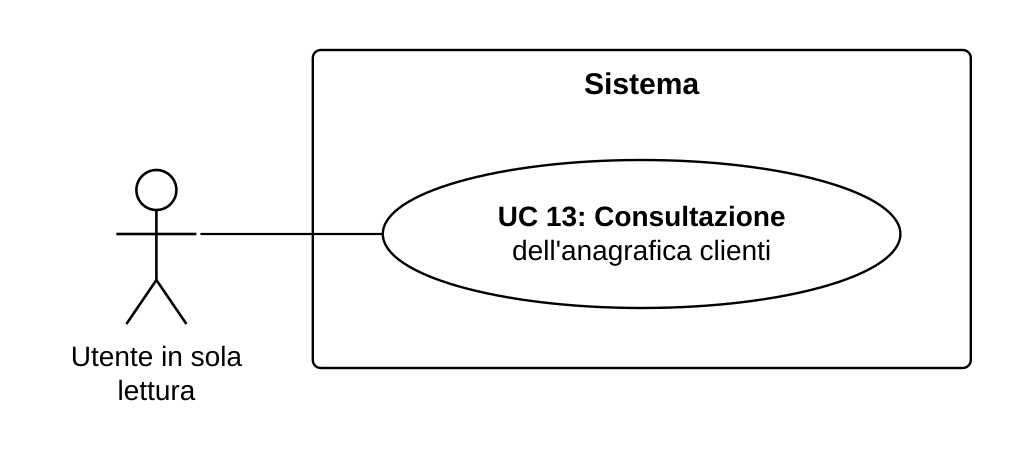
\includegraphics[width=\linewidth,height=0.32\textheight,keepaspectratio]{img/UC13.png}
\caption{UC 13 -- Consultazione dell'anagrafica clienti}
\end{center}
\begin{itemize}
    \item \textbf{Attore principale}: Utente in sola lettura
    \item \textbf{Precondizioni}: L'utente è autenticato.
    \item \textbf{Scenario principale}:
    \begin{enumerate}
        \item L'utente seleziona la consultazione dell'anagrafica clienti.
        \item Il sistema mostra l'anagrafica caricata.
    \end{enumerate}
    \item \textbf{Postcondizioni}: L'anagrafica clienti è visualizzata.
    \item \textbf{Trigger}: L'utente vuole consultare l'anagrafica clienti.
\end{itemize}

% ------------------------------------------------------------
% MACROAREA 3 --- ESTRAZIONE DEI DATI MULTIMODALE
% ------------------------------------------------------------
\subsection{Macroarea 3 --- Estrazione dei dati multimodale}

\subsubsection{UC 14: Trascrizione del messaggio vocale}\label{uc:14}
\begin{center}
\captionsetup{type=figure}
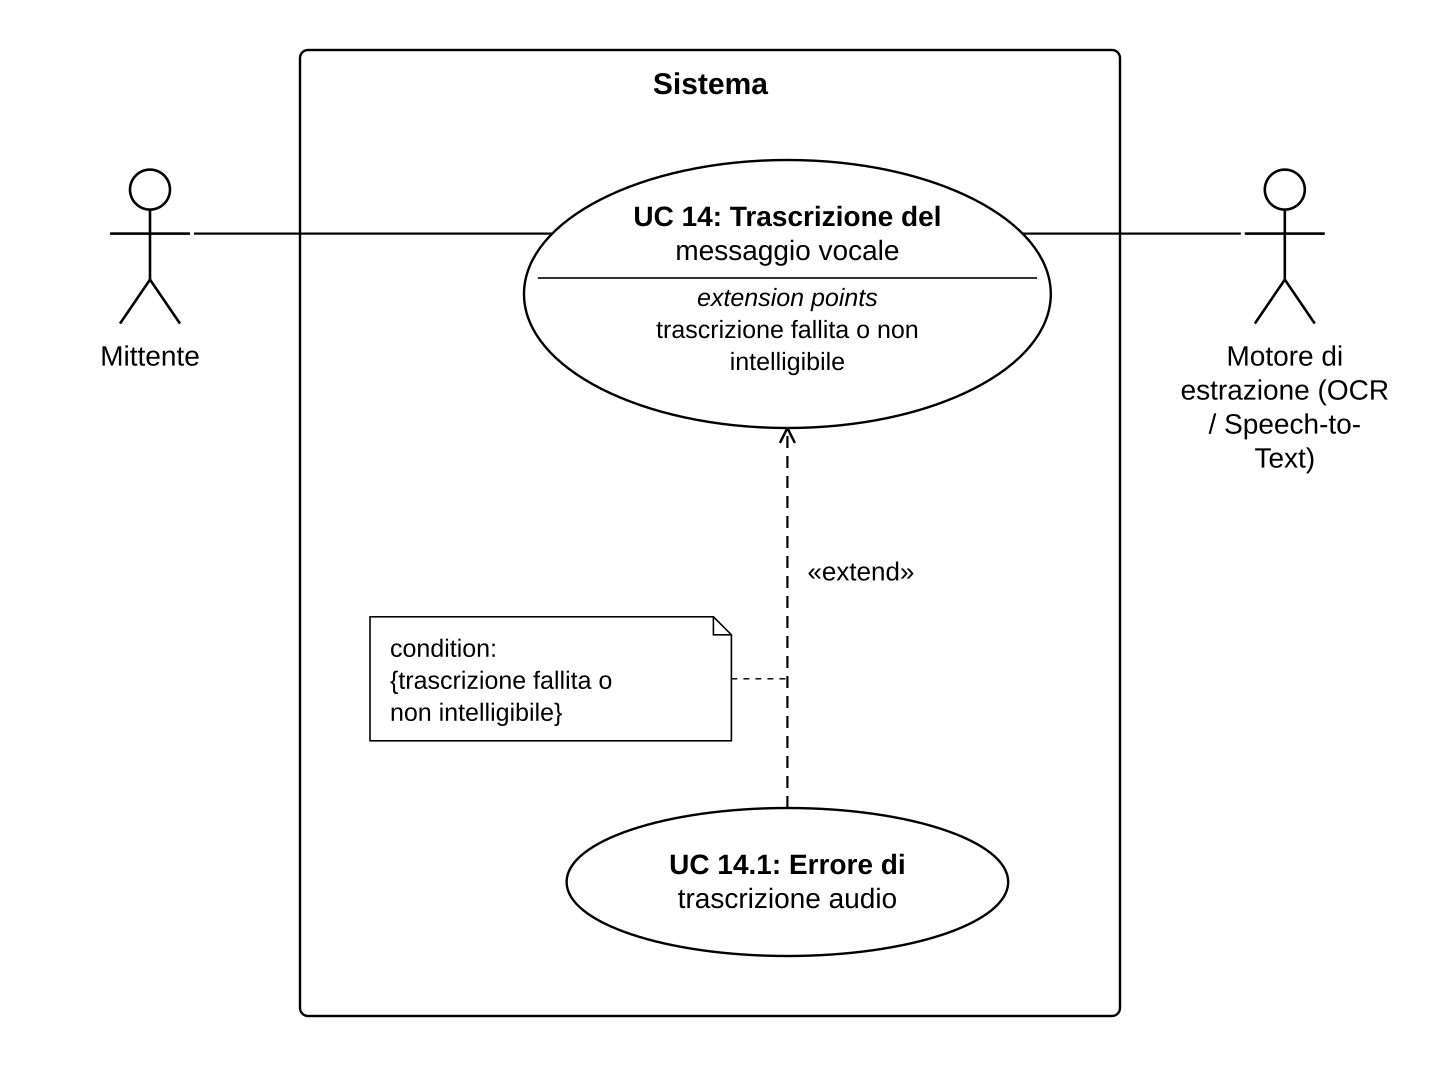
\includegraphics[width=\linewidth,height=0.32\textheight,keepaspectratio]{img/UC14.png}
\caption{UC 14 -- Trascrizione del messaggio vocale}
\end{center}
\begin{itemize}
    \item \textbf{Attore principale}: Mittente
    \item \textbf{Attori secondari}: Motore di estrazione (OCR / Speech-to-Text)
    \item \textbf{Precondizioni}: La richiesta contiene un messaggio vocale.
    \item \textbf{Scenario principale}:
    \begin{enumerate}
        \item Il sistema invia il file audio al motore di trascrizione.
        \item Il motore restituisce il testo trascritto.
        \item Il sistema associa la trascrizione alla richiesta.
    \end{enumerate}
    \item \textbf{Postcondizioni}: Il testo trascritto è associato alla richiesta.
    \item \textbf{Trigger}: Presenza di un messaggio vocale da elaborare.
    \item \textbf{Estensioni}:
    \begin{itemize}
        \item \hyperref[uc:14.1]{UC 14.1}: Errore di trascrizione audio $\rightarrow$ Condizione: Trascrizione fallita o non intelligibile.
    \end{itemize}
\end{itemize}

\subsubsection{UC 14.1: Errore di trascrizione audio}\label{uc:14.1}
\begin{center}
\captionsetup{type=figure}
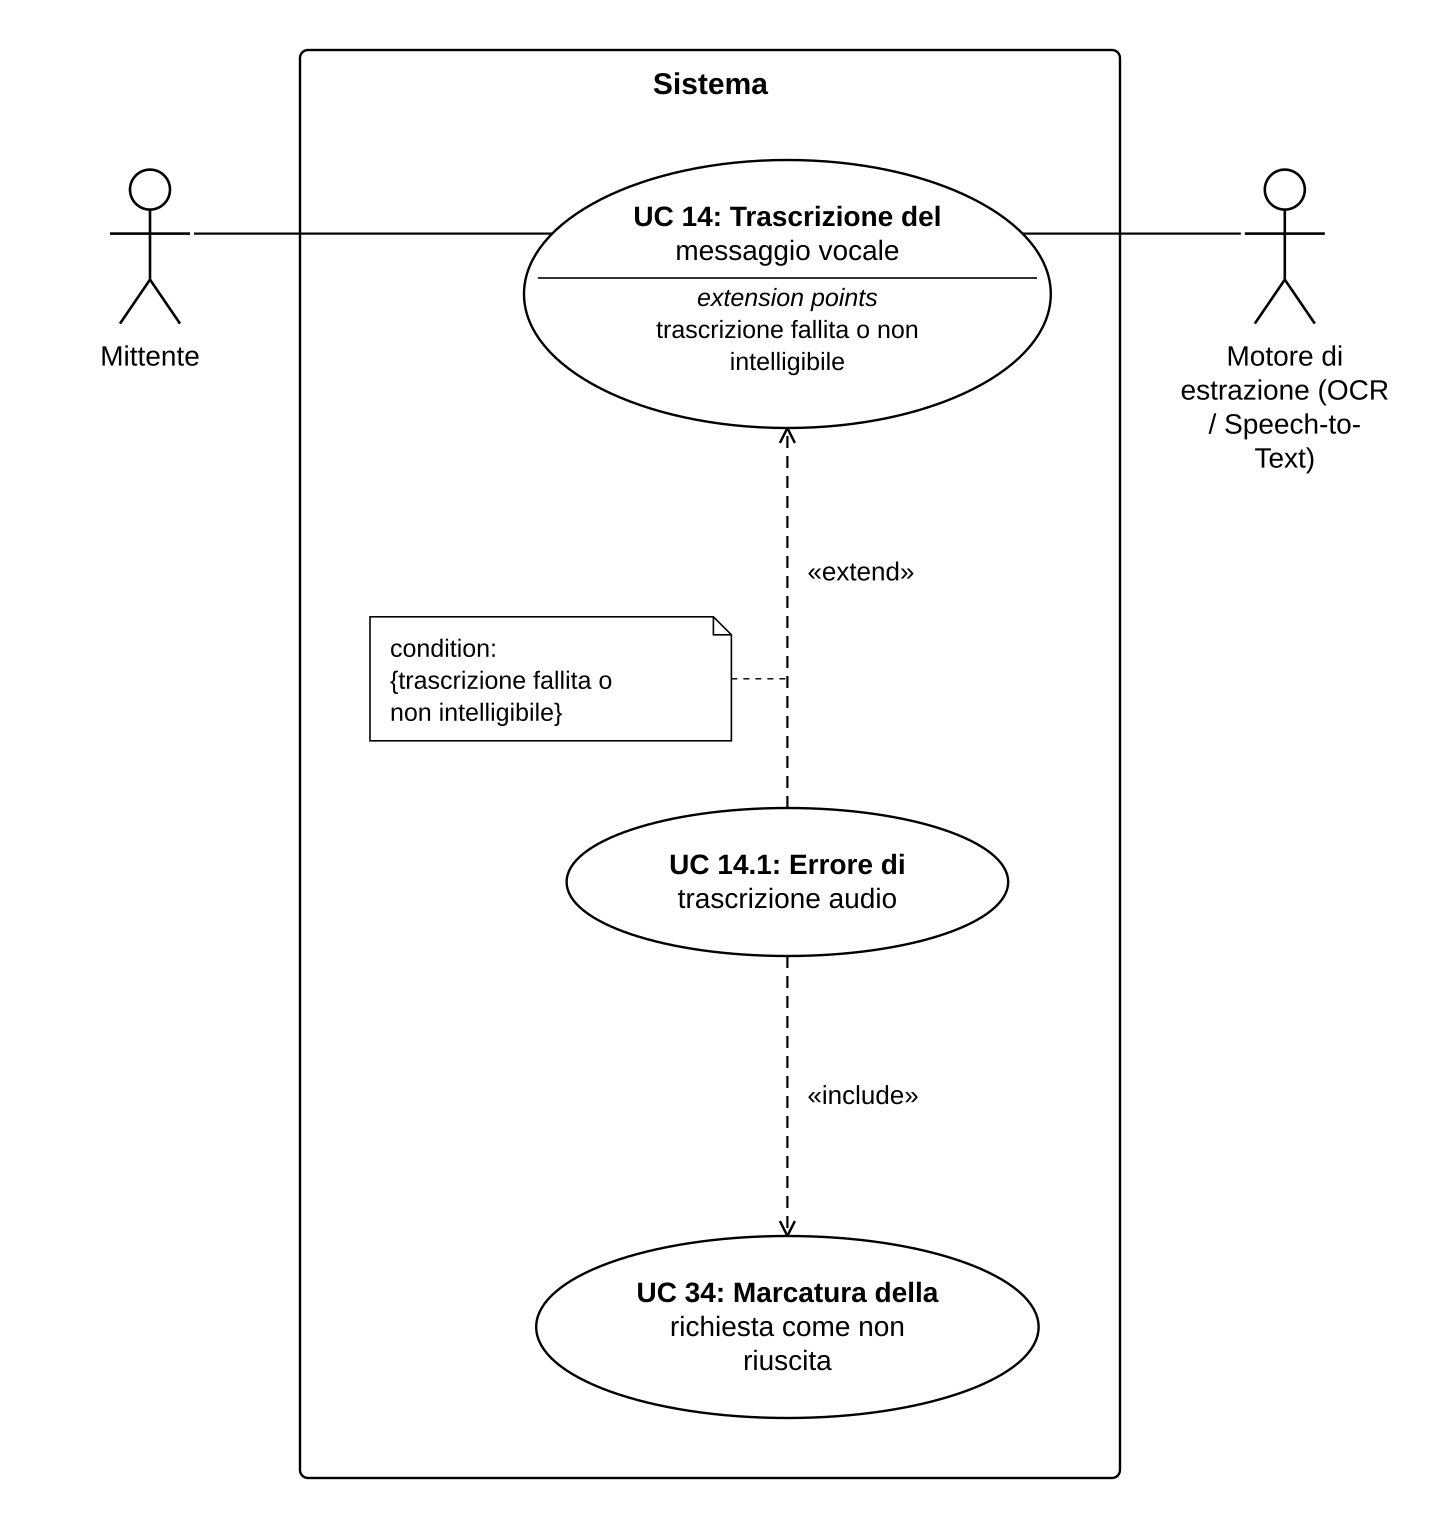
\includegraphics[width=\linewidth,height=0.32\textheight,keepaspectratio]{img/UC14_1.png}
\caption{UC 14.1 -- Errore di trascrizione audio}
\end{center}
\begin{itemize}
    \item \textbf{Attore principale}: Mittente
    \item \textbf{Precondizioni}: La trascrizione audio è in corso.
    \item \textbf{Scenario principale}:
    \begin{enumerate}
        \item Il sistema rileva che la trascrizione è fallita o non è intelligibile.
        \item Il sistema marca la richiesta come non riuscita (\hyperref[uc:34]{UC 34}).
        \item Il sistema registra l'anomalia nei log (\hyperref[uc:37]{UC 37}).
    \end{enumerate}
    \item \textbf{Postcondizioni}: La richiesta è marcata come non riuscita e l'anomalia è registrata nei log.
    \item \textbf{Trigger}: Trascrizione audio fallita o non intelligibile.
    \item \textbf{Estende}: \hyperref[uc:14]{UC 14}.
    \item \textbf{Inclusioni}:
    \begin{itemize}
        \item \hyperref[uc:34]{UC 34}: Marcatura della richiesta come non riuscita
    \end{itemize}
\end{itemize}

\subsubsection{UC 15: Estrazione del testo da immagine allegata}\label{uc:15}
\begin{center}
\captionsetup{type=figure}
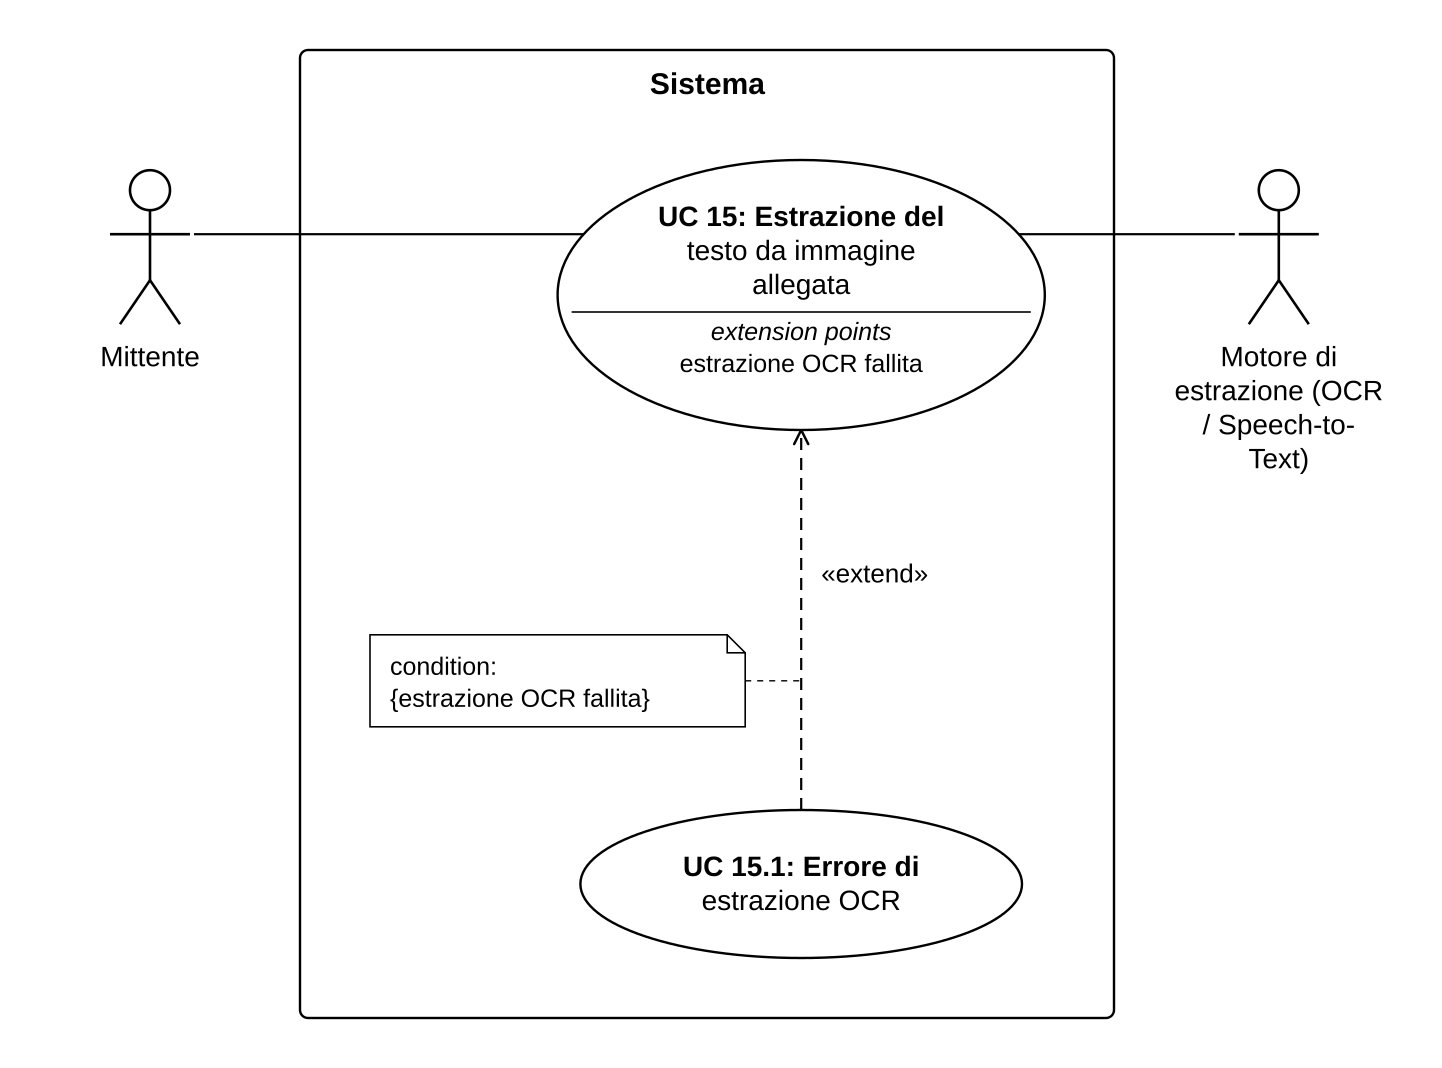
\includegraphics[width=\linewidth,height=0.32\textheight,keepaspectratio]{img/UC15.png}
\caption{UC 15 -- Estrazione del testo da immagine allegata}
\end{center}
\begin{itemize}
    \item \textbf{Attore principale}: Mittente
    \item \textbf{Attori secondari}: Motore di estrazione (OCR / Speech-to-Text)
    \item \textbf{Precondizioni}: La richiesta contiene un'immagine allegata a un'e-mail.
    \item \textbf{Scenario principale}:
    \begin{enumerate}
        \item Il sistema invia l'immagine al motore OCR.
        \item Il motore restituisce il testo estratto.
        \item Il sistema associa il testo estratto alla richiesta.
    \end{enumerate}
    \item \textbf{Postcondizioni}: Il testo estratto è associato alla richiesta.
    \item \textbf{Trigger}: Presenza di un'immagine allegata da elaborare.
    \item \textbf{Estensioni}:
    \begin{itemize}
        \item \hyperref[uc:15.1]{UC 15.1}: Errore di estrazione OCR $\rightarrow$ Condizione: Estrazione OCR fallita.
    \end{itemize}
\end{itemize}

\subsubsection{UC 15.1: Errore di estrazione OCR}\label{uc:15.1}
\begin{center}
\captionsetup{type=figure}
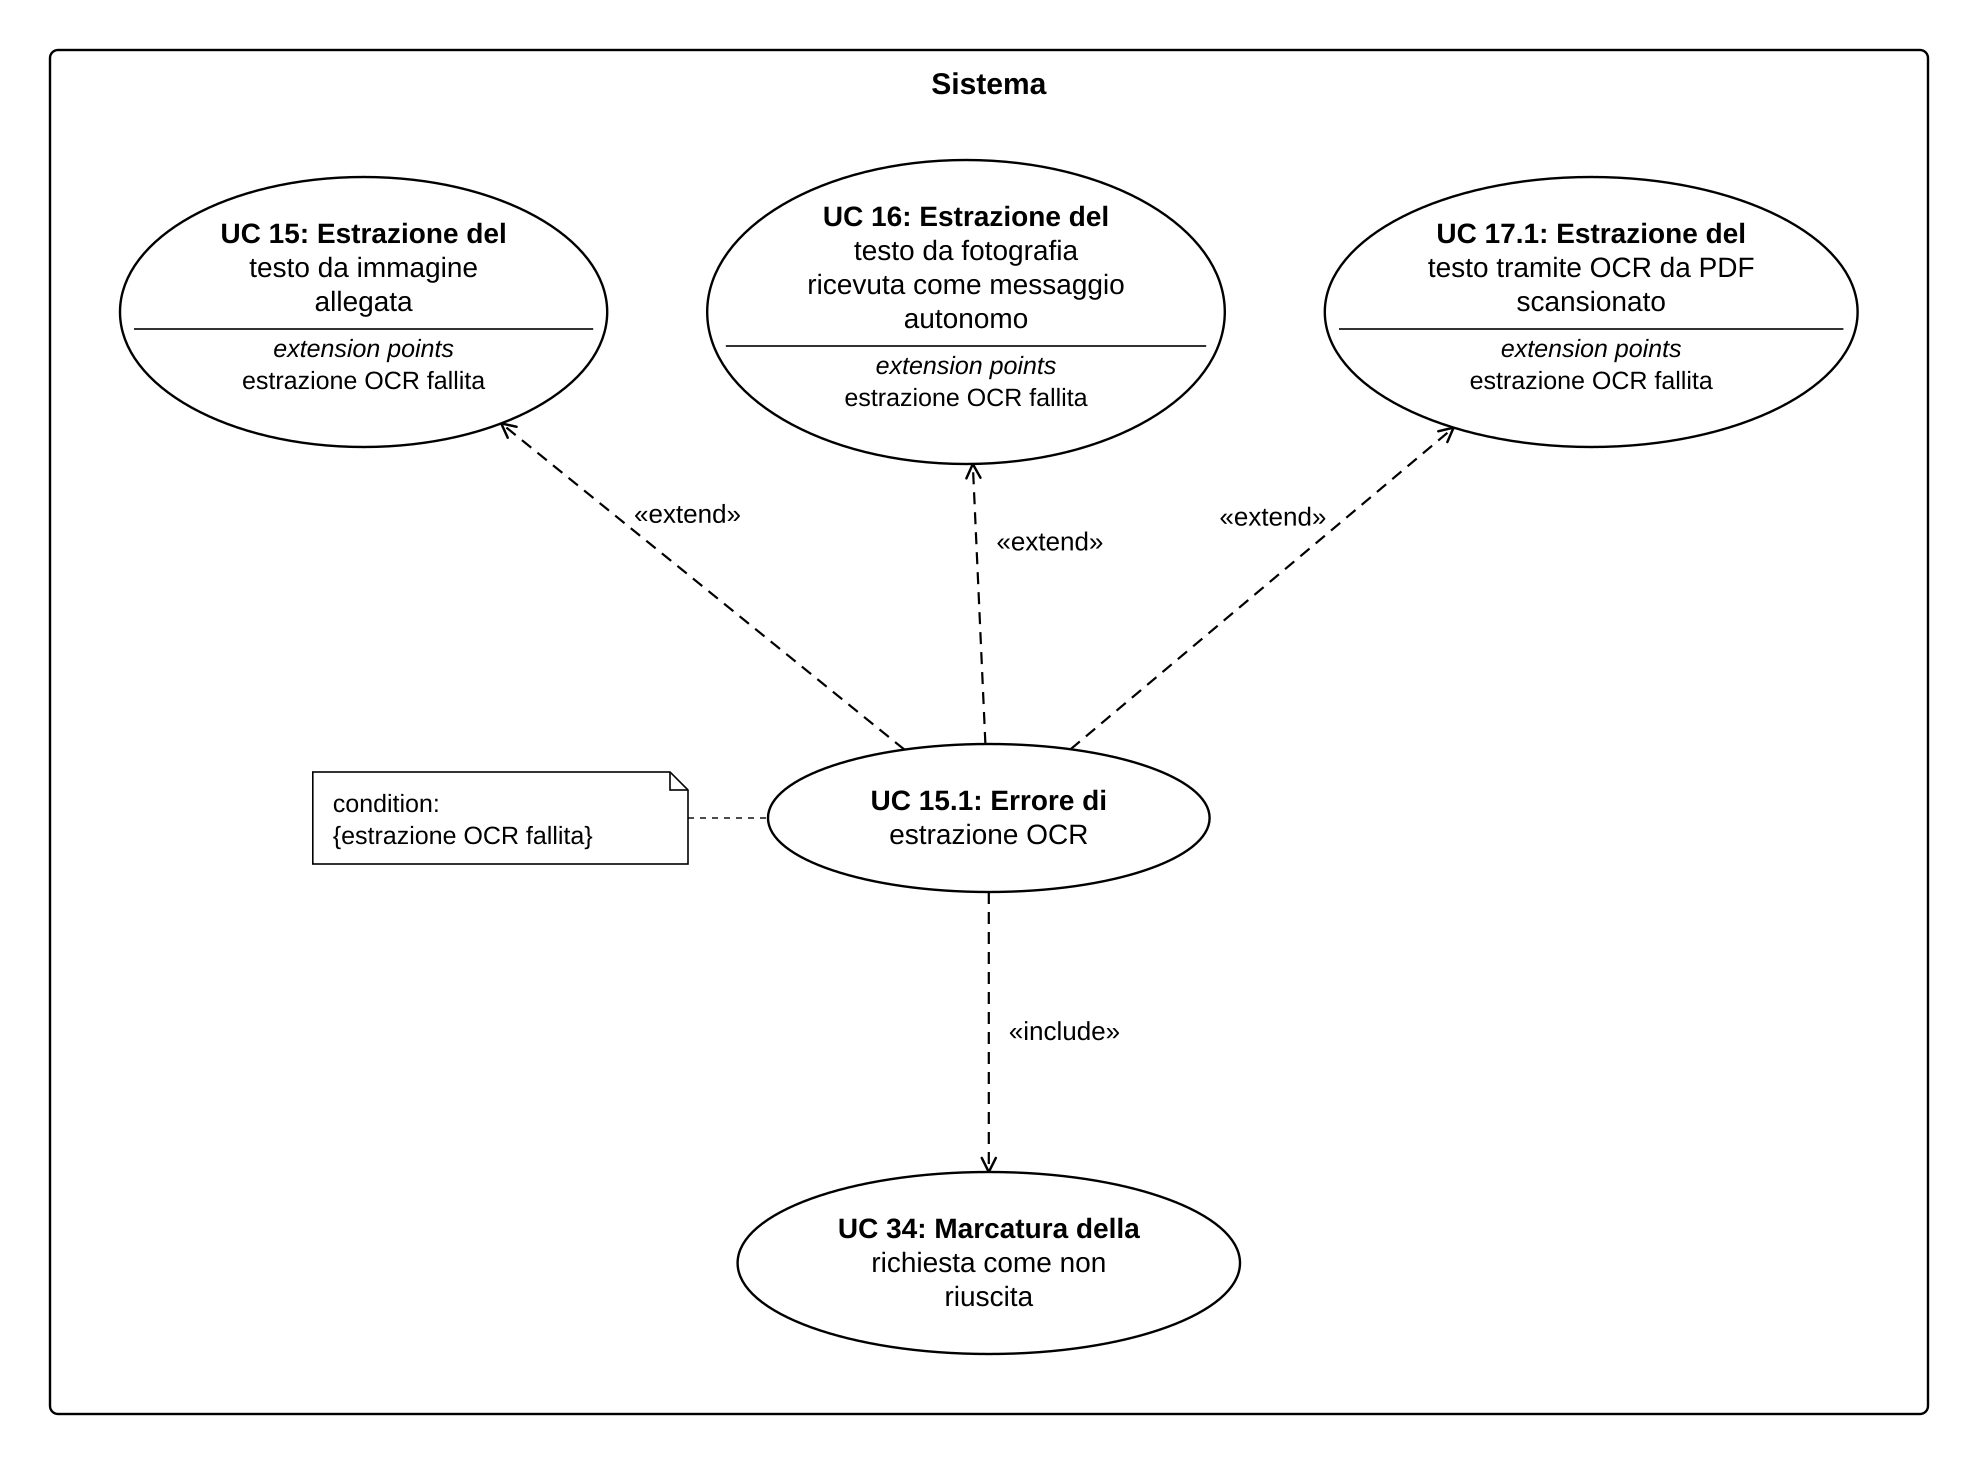
\includegraphics[width=\linewidth,height=0.32\textheight,keepaspectratio]{img/UC15_1.png}
\caption{UC 15.1 -- Errore di estrazione OCR}
\end{center}
\begin{itemize}
    \item \textbf{Attore principale}: Mittente
    \item \textbf{Precondizioni}: L'estrazione del testo tramite OCR è in corso.
    \item \textbf{Scenario principale}:
    \begin{enumerate}
        \item Il sistema rileva che l'estrazione OCR è fallita.
        \item Il sistema marca la richiesta come non riuscita (\hyperref[uc:34]{UC 34}).
        \item Il sistema registra l'anomalia nei log (\hyperref[uc:37]{UC 37}).
    \end{enumerate}
    \item \textbf{Postcondizioni}: La richiesta è marcata come non riuscita e l'anomalia è registrata nei log.
    \item \textbf{Trigger}: Estrazione OCR fallita.
    \item \textbf{Estende}: \hyperref[uc:15]{UC 15}, \hyperref[uc:16]{UC 16}, \hyperref[uc:17.1]{UC 17.1}.
    \item \textbf{Inclusioni}:
    \begin{itemize}
        \item \hyperref[uc:34]{UC 34}: Marcatura della richiesta come non riuscita
    \end{itemize}
\end{itemize}

\subsubsection{UC 16: Estrazione del testo da fotografia ricevuta come messaggio autonomo}\label{uc:16}
\begin{center}
\captionsetup{type=figure}
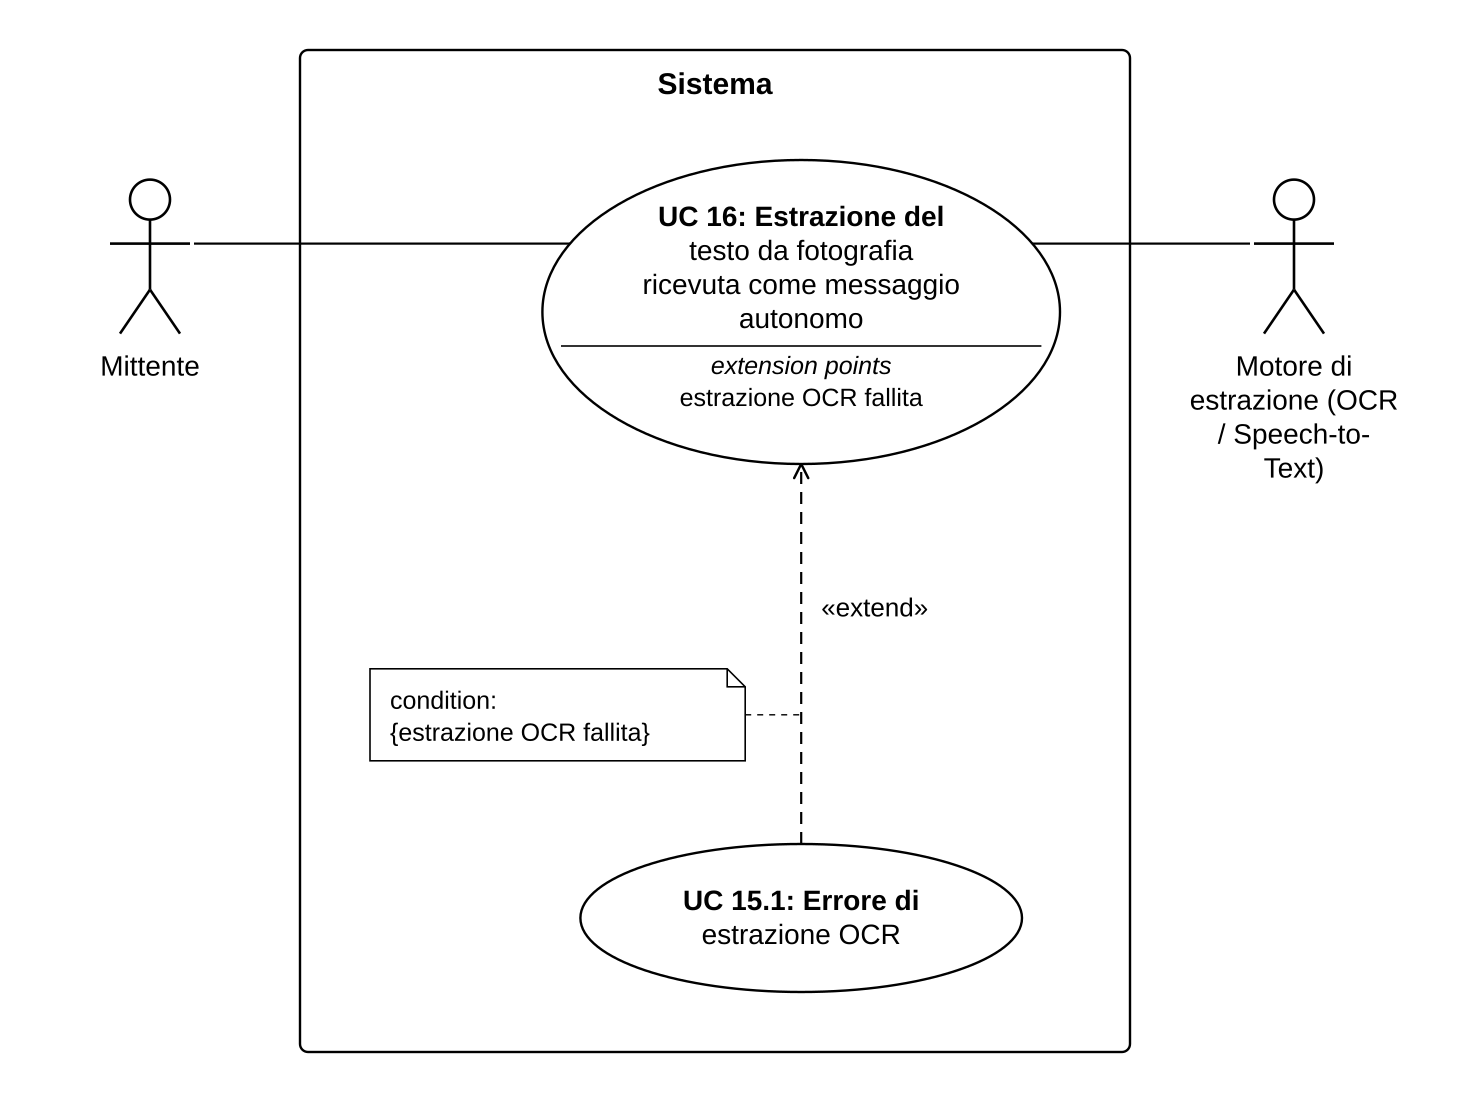
\includegraphics[width=\linewidth,height=0.32\textheight,keepaspectratio]{img/UC16.png}
\caption{UC 16 -- Estrazione del testo da fotografia ricevuta come messaggio autonomo}
\end{center}
\begin{itemize}
    \item \textbf{Attore principale}: Mittente
    \item \textbf{Attori secondari}: Motore di estrazione (OCR / Speech-to-Text)
    \item \textbf{Precondizioni}: La richiesta è costituita da una fotografia ricevuta come messaggio autonomo.
    \item \textbf{Scenario principale}:
    \begin{enumerate}
        \item Il sistema invia la fotografia al motore OCR.
        \item Il motore restituisce il testo estratto.
        \item Il sistema associa il testo estratto alla richiesta.
    \end{enumerate}
    \item \textbf{Postcondizioni}: Il testo estratto è associato alla richiesta.
    \item \textbf{Trigger}: Ricezione di una fotografia come messaggio autonomo.
    \item \textbf{Estensioni}:
    \begin{itemize}
        \item \hyperref[uc:15.1]{UC 15.1}: Errore di estrazione OCR $\rightarrow$ Condizione: Estrazione OCR fallita.
    \end{itemize}
\end{itemize}

\subsubsection{UC 17: Estrazione del testo da allegato PDF}\label{uc:17}
\begin{center}
\captionsetup{type=figure}
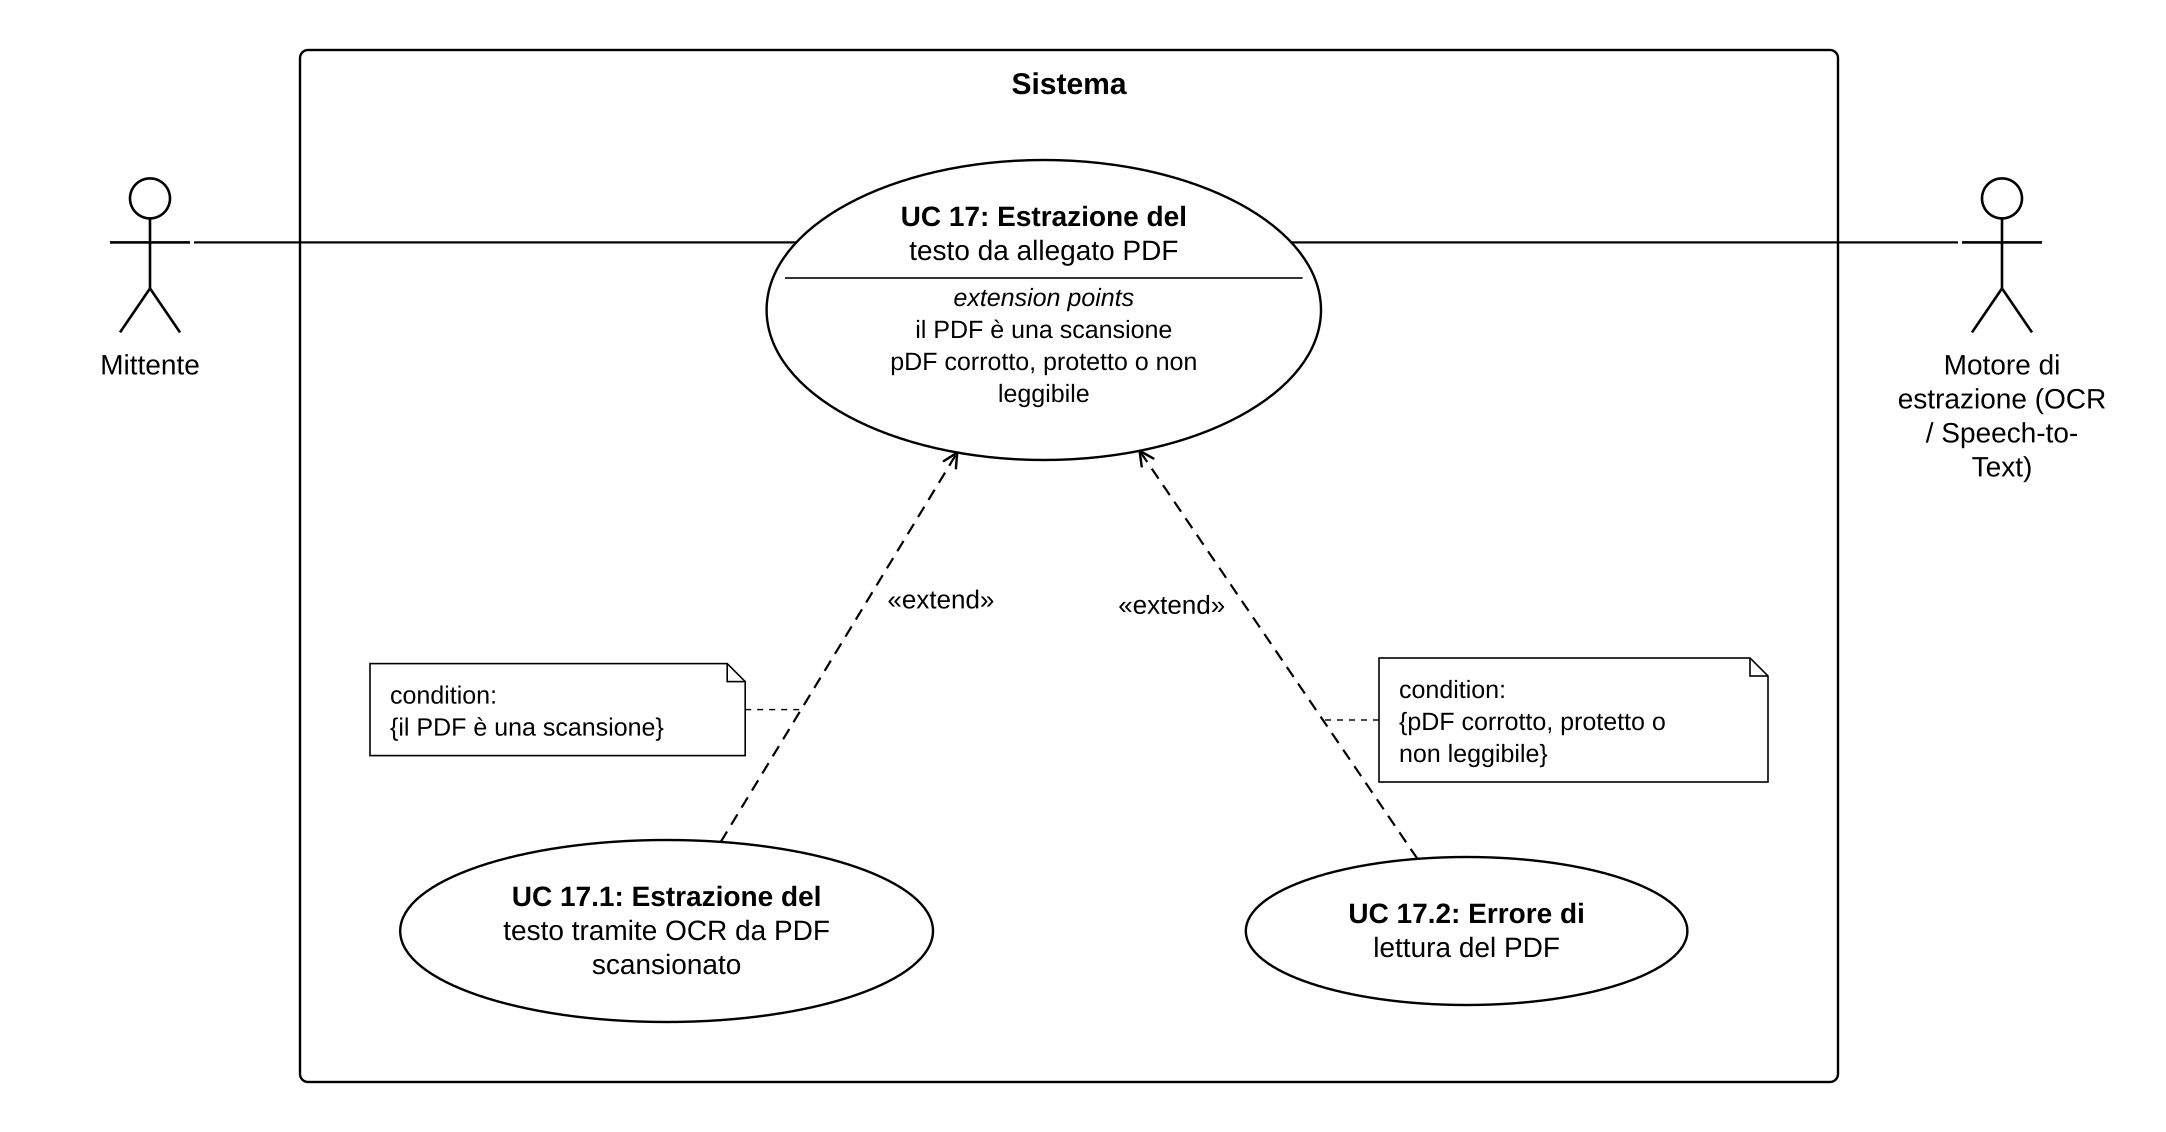
\includegraphics[width=\linewidth,height=0.32\textheight,keepaspectratio]{img/UC17.png}
\caption{UC 17 -- Estrazione del testo da allegato PDF}
\end{center}
\begin{itemize}
    \item \textbf{Attore principale}: Mittente
    \item \textbf{Attori secondari}: Motore di estrazione (OCR / Speech-to-Text)
    \item \textbf{Precondizioni}: La richiesta contiene un allegato PDF.
    \item \textbf{Scenario principale}:
    \begin{enumerate}
        \item Il sistema legge il contenuto del PDF.
        \item Il sistema estrae il testo del documento.
        \item Il sistema associa il testo estratto alla richiesta.
    \end{enumerate}
    \item \textbf{Postcondizioni}: Il testo del PDF è associato alla richiesta.
    \item \textbf{Trigger}: Presenza di un allegato PDF da elaborare.
    \item \textbf{Estensioni}:
    \begin{itemize}
        \item \hyperref[uc:17.1]{UC 17.1}: Estrazione del testo tramite OCR da PDF scansionato $\rightarrow$ Condizione: Il PDF è una scansione.
        \item \hyperref[uc:17.2]{UC 17.2}: Errore di lettura del PDF $\rightarrow$ Condizione: PDF corrotto, protetto o non leggibile.
    \end{itemize}
\end{itemize}

\subsubsection{UC 17.1: Estrazione del testo tramite OCR da PDF scansionato}\label{uc:17.1}
\begin{center}
\captionsetup{type=figure}
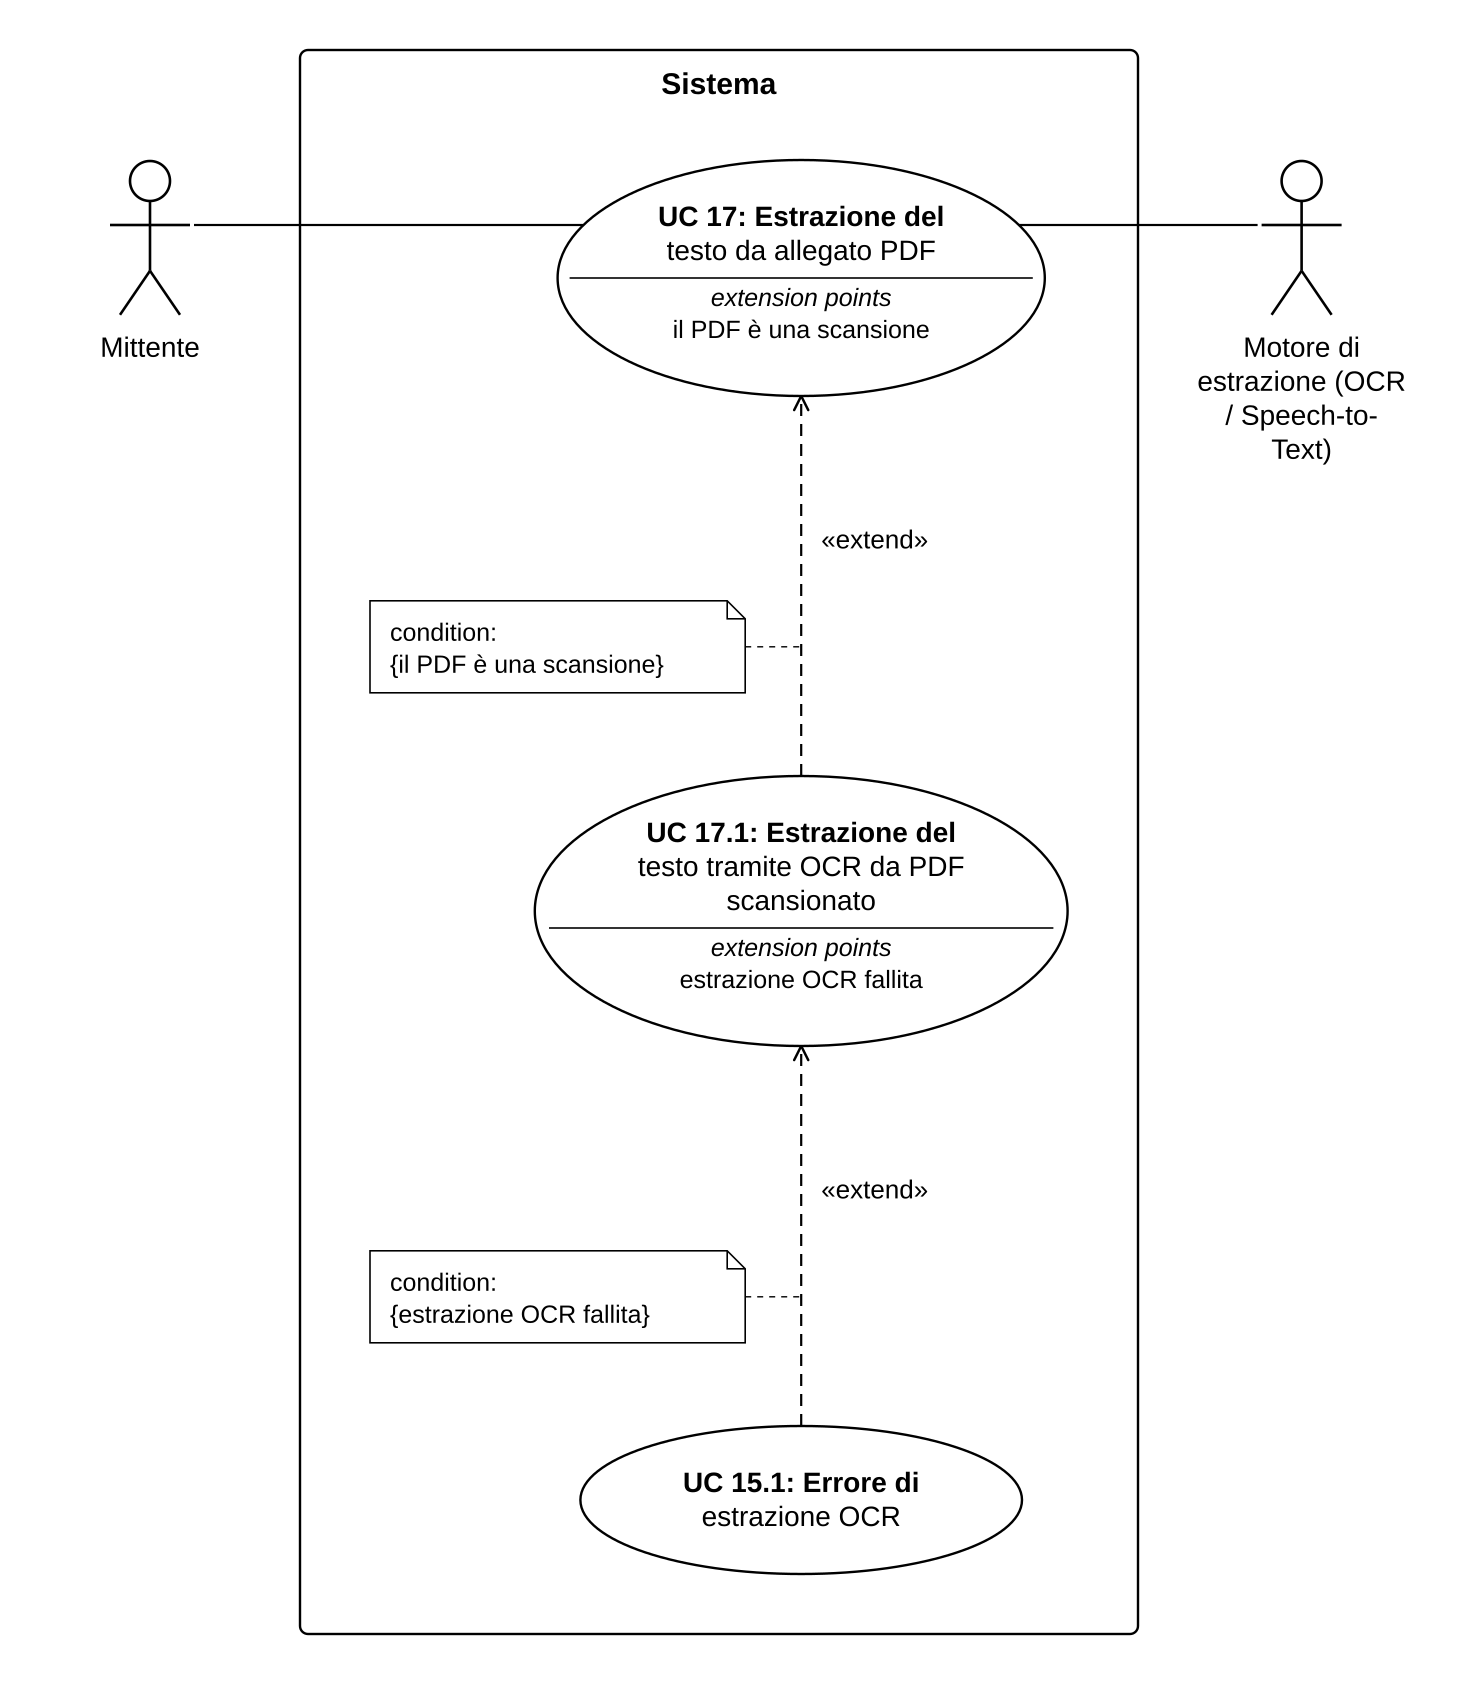
\includegraphics[width=\linewidth,height=0.32\textheight,keepaspectratio]{img/UC17_1.png}
\caption{UC 17.1 -- Estrazione del testo tramite OCR da PDF scansionato}
\end{center}
\begin{itemize}
    \item \textbf{Attore principale}: Mittente
    \item \textbf{Precondizioni}: L'estrazione del testo da un PDF è in corso.
    \item \textbf{Scenario principale}:
    \begin{enumerate}
        \item Il sistema rileva che il PDF è una scansione priva di testo selezionabile.
        \item Il sistema invia le pagine al motore OCR.
        \item Il motore restituisce il testo estratto.
    \end{enumerate}
    \item \textbf{Postcondizioni}: Il testo del PDF scansionato è estratto.
    \item \textbf{Trigger}: Il PDF allegato è una scansione.
    \item \textbf{Estende}: \hyperref[uc:17]{UC 17}.
    \item \textbf{Estensioni}:
    \begin{itemize}
        \item \hyperref[uc:15.1]{UC 15.1}: Errore di estrazione OCR $\rightarrow$ Condizione: Estrazione OCR fallita.
    \end{itemize}
\end{itemize}

\subsubsection{UC 17.2: Errore di lettura del PDF}\label{uc:17.2}
\begin{center}
\captionsetup{type=figure}
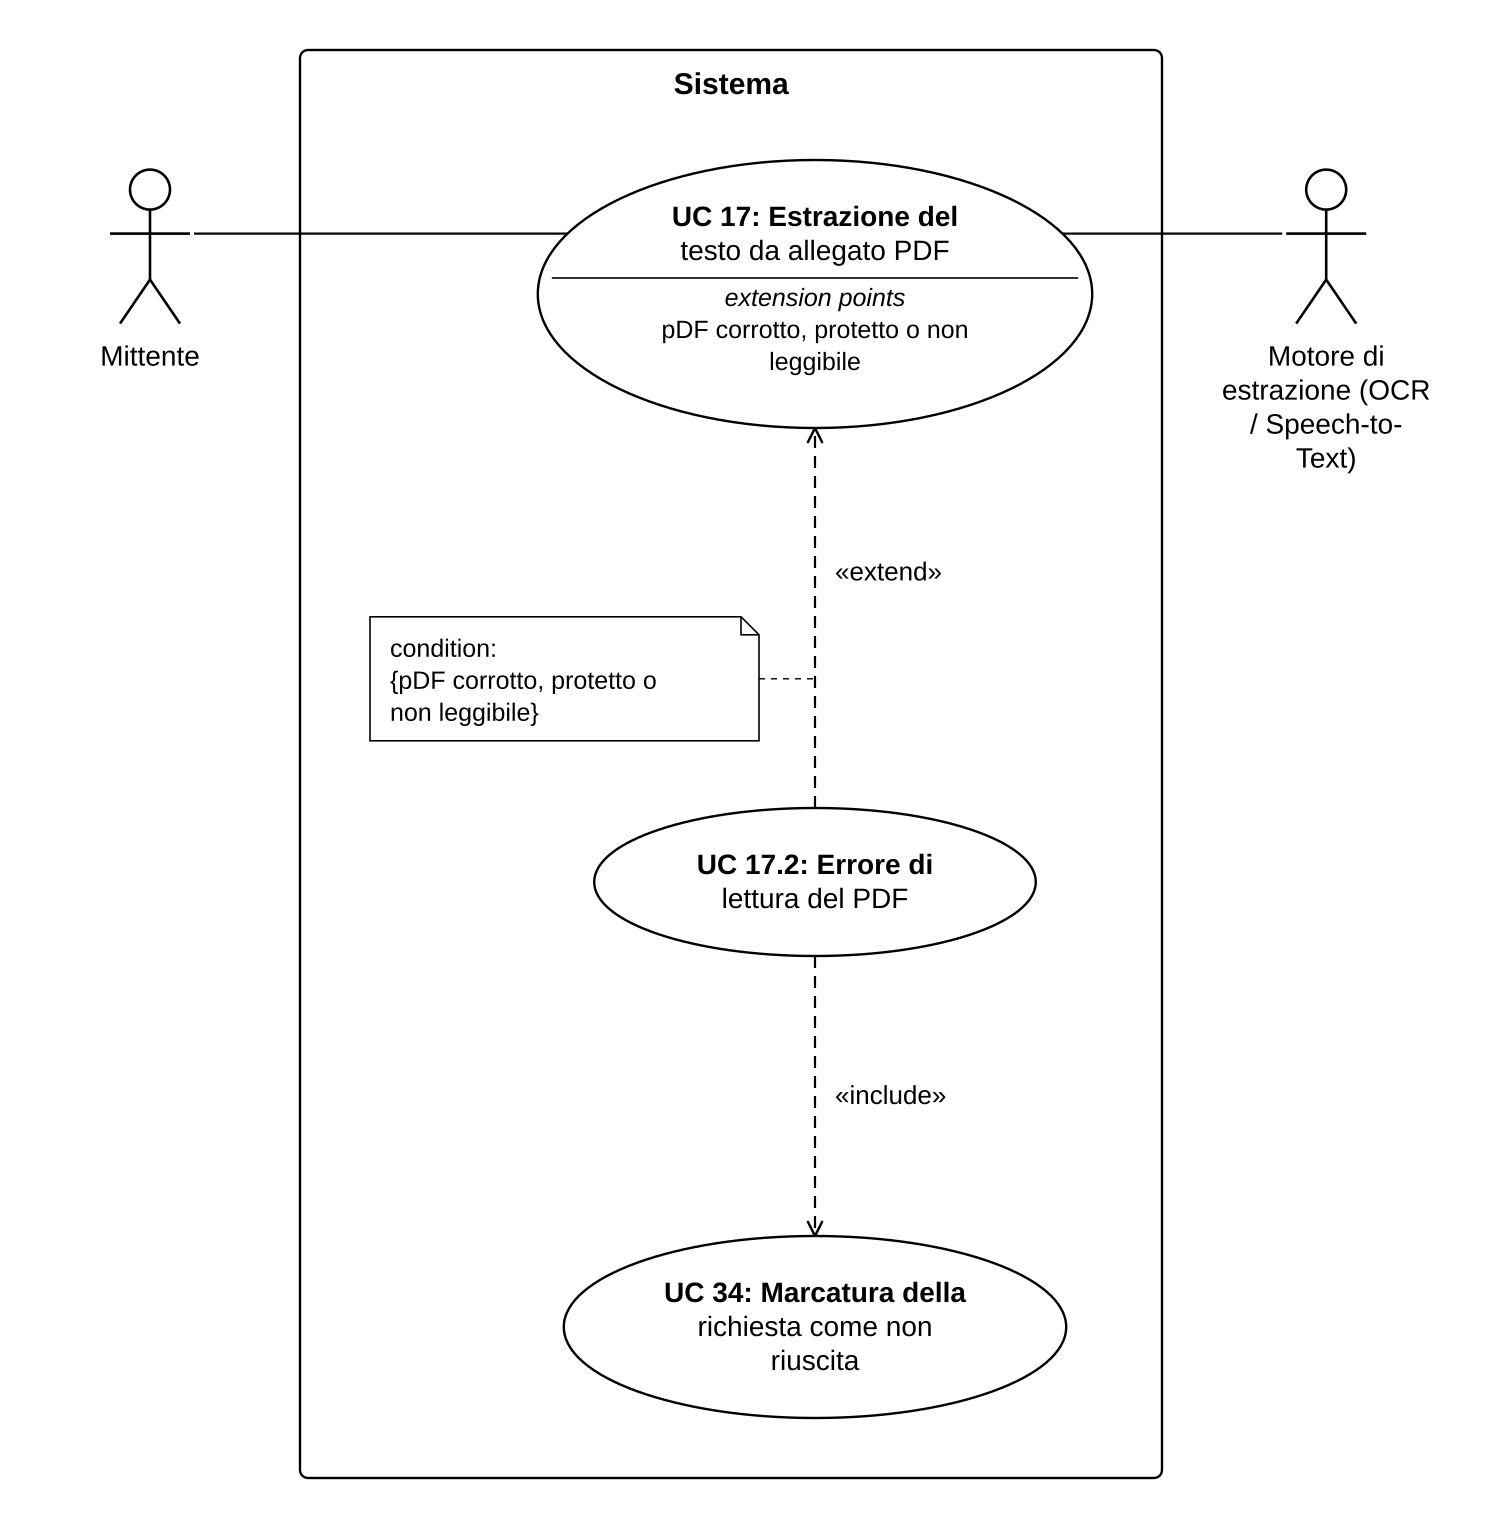
\includegraphics[width=\linewidth,height=0.32\textheight,keepaspectratio]{img/UC17_2.png}
\caption{UC 17.2 -- Errore di lettura del PDF}
\end{center}
\begin{itemize}
    \item \textbf{Attore principale}: Mittente
    \item \textbf{Precondizioni}: La lettura del PDF è in corso.
    \item \textbf{Scenario principale}:
    \begin{enumerate}
        \item Il sistema rileva che il PDF è corrotto, protetto o non leggibile.
        \item Il sistema marca la richiesta come non riuscita (\hyperref[uc:34]{UC 34}).
        \item Il sistema registra l'anomalia nei log (\hyperref[uc:37]{UC 37}).
    \end{enumerate}
    \item \textbf{Postcondizioni}: La richiesta è marcata come non riuscita e l'anomalia è registrata nei log.
    \item \textbf{Trigger}: PDF corrotto, protetto o non leggibile.
    \item \textbf{Estende}: \hyperref[uc:17]{UC 17}.
    \item \textbf{Inclusioni}:
    \begin{itemize}
        \item \hyperref[uc:34]{UC 34}: Marcatura della richiesta come non riuscita
    \end{itemize}
\end{itemize}

\subsubsection{UC 18: Raffinamento dell'estrazione tramite LLM}\label{uc:18}
\begin{center}
\captionsetup{type=figure}
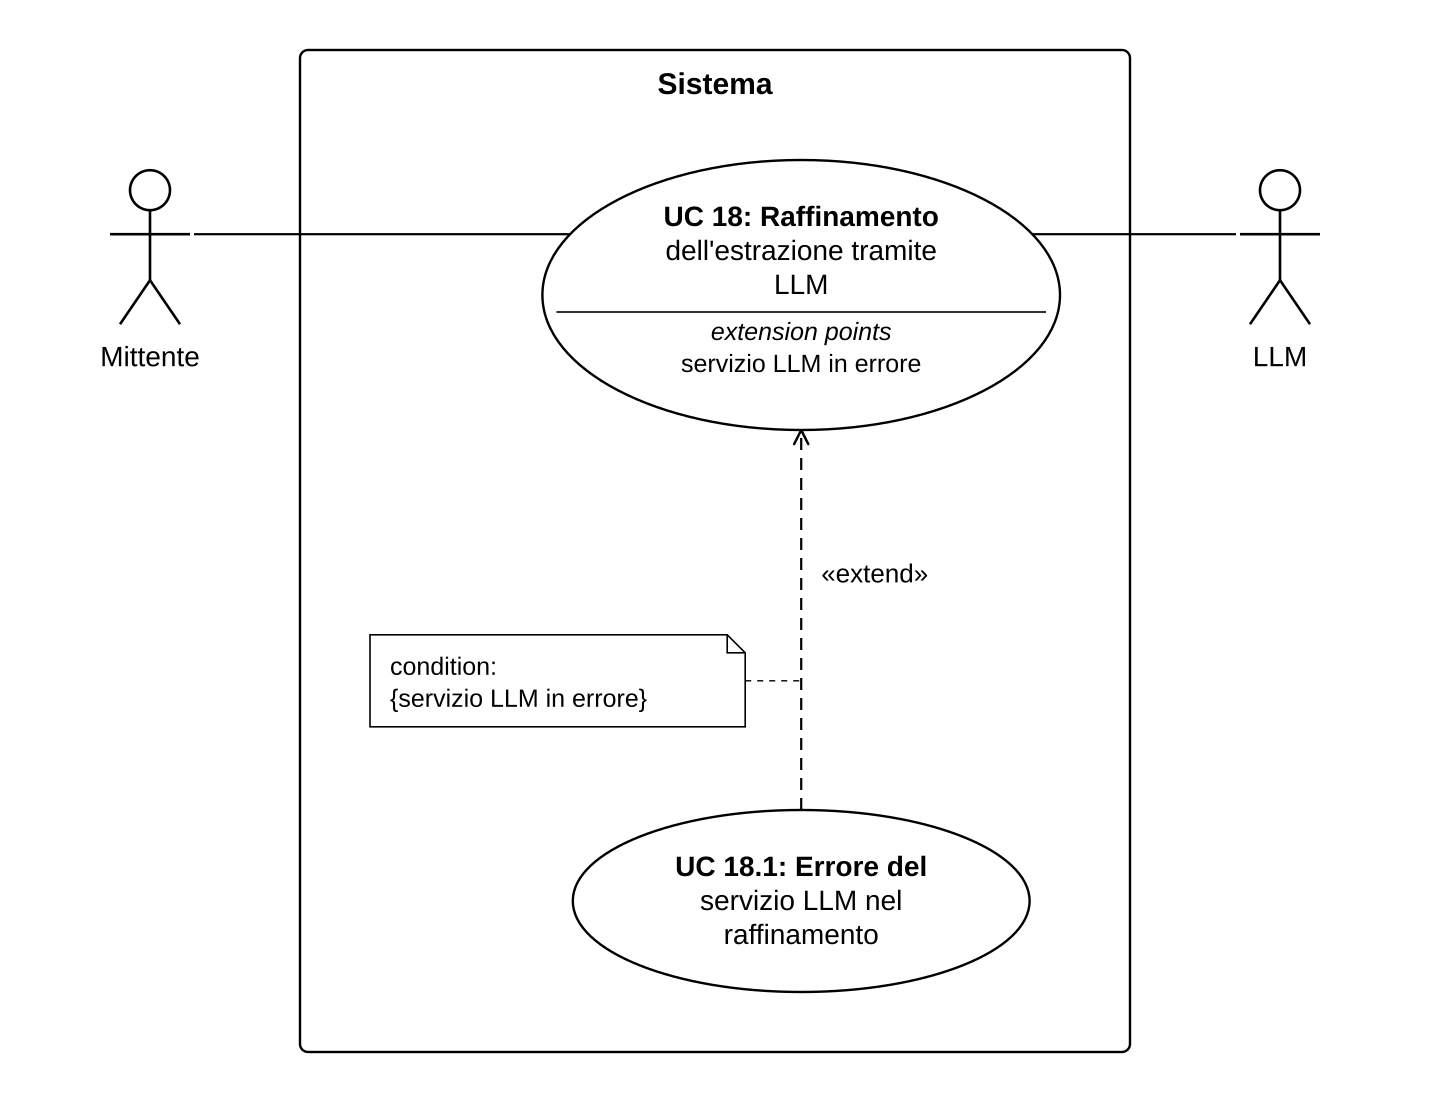
\includegraphics[width=\linewidth,height=0.32\textheight,keepaspectratio]{img/UC18.png}
\caption{UC 18 -- Raffinamento dell'estrazione tramite LLM}
\end{center}
\begin{itemize}
    \item \textbf{Attore principale}: Mittente
    \item \textbf{Attori secondari}: LLM
    \item \textbf{Precondizioni}: È disponibile un testo estratto da OCR o trascrizione e il servizio LLM è raggiungibile.
    \item \textbf{Scenario principale}:
    \begin{enumerate}
        \item Il sistema invia all'LLM i dati ottenuti dall'estrazione iniziale.
        \item L'LLM migliora la scansione o completa l'estrazione incompleta.
        \item Il sistema sostituisce i dati iniziali con quelli raffinati.
    \end{enumerate}
    \item \textbf{Postcondizioni}: I dati estratti sono raffinati.
    \item \textbf{Trigger}: Completamento della prima fase di estrazione.
    \item \textbf{Estensioni}:
    \begin{itemize}
        \item \hyperref[uc:18.1]{UC 18.1}: Errore del servizio LLM nel raffinamento $\rightarrow$ Condizione: Servizio LLM in errore.
    \end{itemize}
\end{itemize}

\subsubsection{UC 18.1: Errore del servizio LLM nel raffinamento}\label{uc:18.1}
\begin{center}
\captionsetup{type=figure}
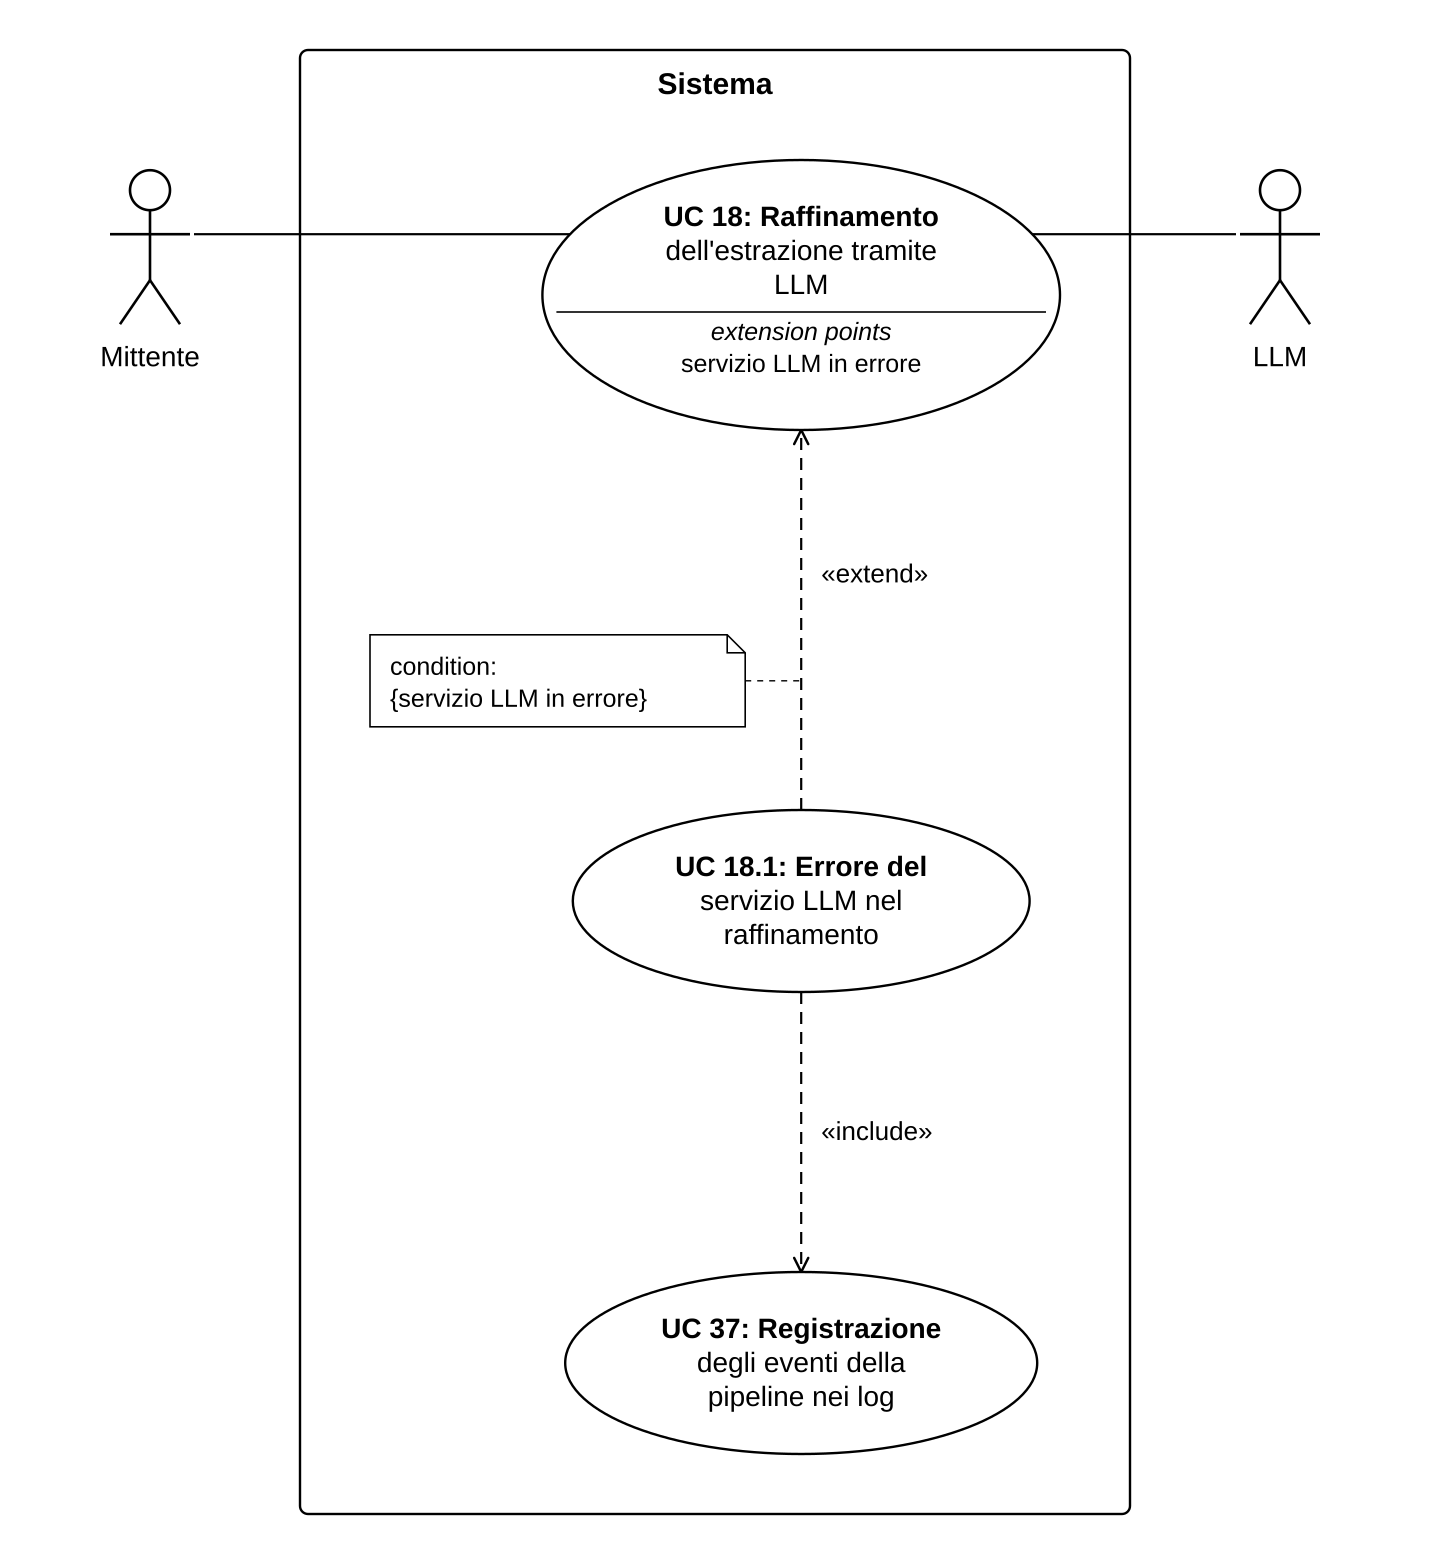
\includegraphics[width=\linewidth,height=0.32\textheight,keepaspectratio]{img/UC18_1.png}
\caption{UC 18.1 -- Errore del servizio LLM nel raffinamento}
\end{center}
\begin{itemize}
    \item \textbf{Attore principale}: Mittente
    \item \textbf{Precondizioni}: Il raffinamento tramite LLM è in corso.
    \item \textbf{Scenario principale}:
    \begin{enumerate}
        \item Il sistema rileva un errore del servizio LLM.
        \item Il sistema mantiene i dati dell'estrazione iniziale.
        \item Il sistema registra l'errore nei log (\hyperref[uc:37]{UC 37}).
    \end{enumerate}
    \item \textbf{Postcondizioni}: I dati dell'estrazione iniziale sono conservati e l'errore è registrato nei log.
    \item \textbf{Trigger}: Errore del servizio LLM durante il raffinamento.
    \item \textbf{Estende}: \hyperref[uc:18]{UC 18}.
    \item \textbf{Inclusioni}:
    \begin{itemize}
        \item \hyperref[uc:37]{UC 37}: Registrazione degli eventi della pipeline nei log
    \end{itemize}
\end{itemize}

\subsubsection{UC 19: Valutazione dell'affidabilità rispetto alla soglia di confidenza}\label{uc:19}
\begin{center}
\captionsetup{type=figure}
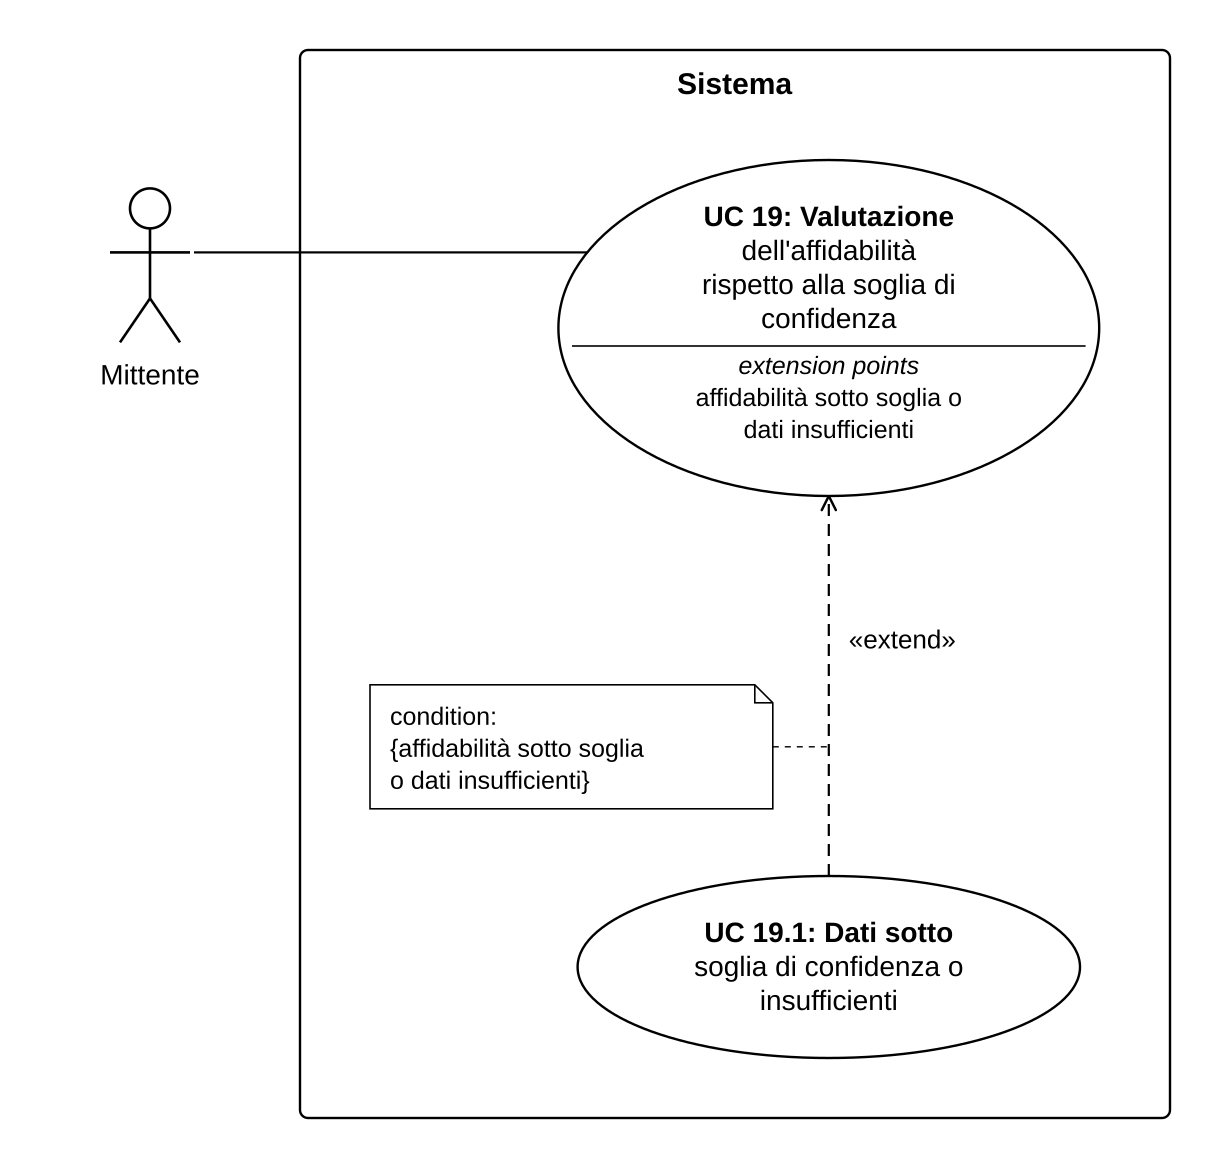
\includegraphics[width=\linewidth,height=0.32\textheight,keepaspectratio]{img/UC19.png}
\caption{UC 19 -- Valutazione dell'affidabilità rispetto alla soglia di confidenza}
\end{center}
\begin{itemize}
    \item \textbf{Attore principale}: Mittente
    \item \textbf{Precondizioni}: I dati sono stati estratti e la soglia di confidenza è configurata.
    \item \textbf{Scenario principale}:
    \begin{enumerate}
        \item Il sistema calcola l'affidabilità dei dati estratti.
        \item Il sistema confronta l'affidabilità con la soglia di confidenza.
        \item Il sistema stabilisce che l'affidabilità è sufficiente e prosegue.
    \end{enumerate}
    \item \textbf{Postcondizioni}: L'affidabilità dei dati è verificata e la richiesta prosegue.
    \item \textbf{Trigger}: Completamento dell'estrazione dei dati.
    \item \textbf{Estensioni}:
    \begin{itemize}
        \item \hyperref[uc:19.1]{UC 19.1}: Dati sotto soglia di confidenza o insufficienti $\rightarrow$ Condizione: Affidabilità sotto soglia o dati insufficienti.
    \end{itemize}
\end{itemize}

\subsubsection{UC 19.1: Dati sotto soglia di confidenza o insufficienti}\label{uc:19.1}
\begin{center}
\captionsetup{type=figure}
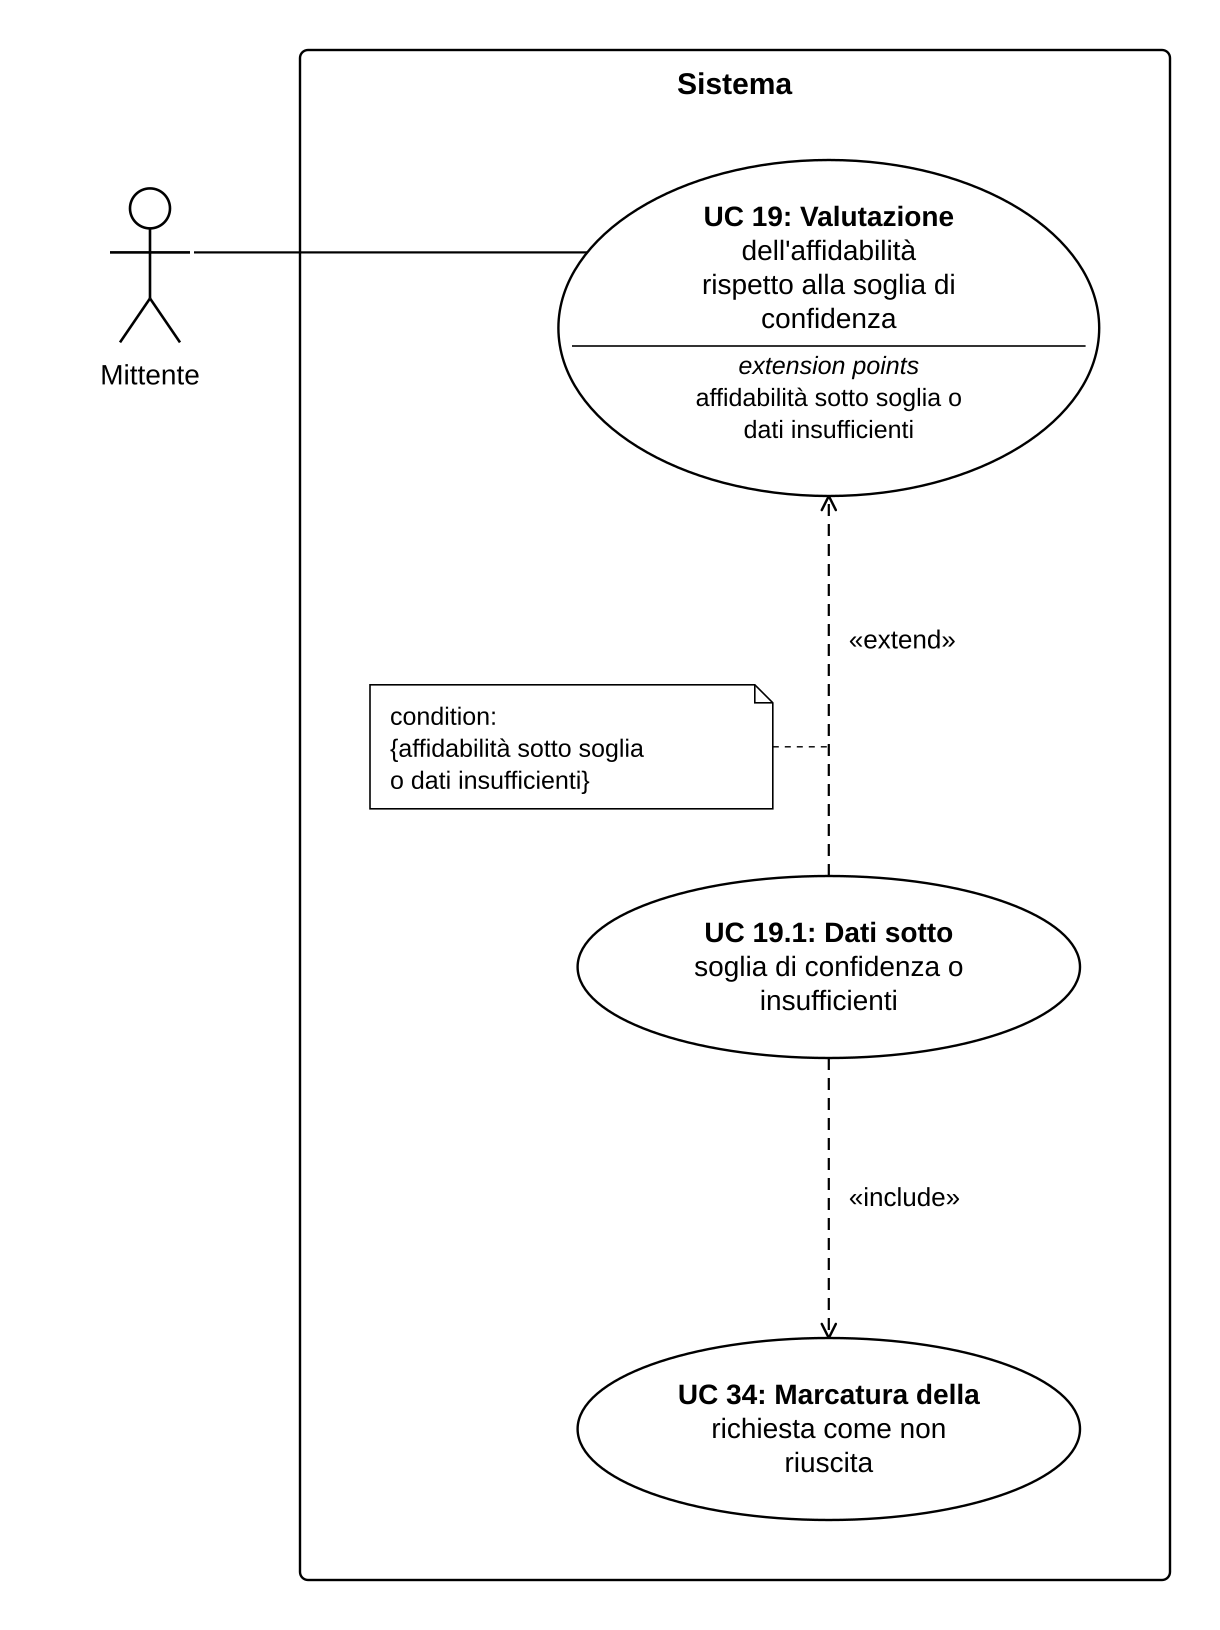
\includegraphics[width=\linewidth,height=0.32\textheight,keepaspectratio]{img/UC19_1.png}
\caption{UC 19.1 -- Dati sotto soglia di confidenza o insufficienti}
\end{center}
\begin{itemize}
    \item \textbf{Attore principale}: Mittente
    \item \textbf{Precondizioni}: La valutazione dell'affidabilità è in corso.
    \item \textbf{Scenario principale}:
    \begin{enumerate}
        \item Il sistema rileva dati sotto la soglia di confidenza o insufficienti.
        \item Il sistema marca la richiesta come non riuscita (\hyperref[uc:34]{UC 34}).
        \item Il sistema registra nei log lo specifico elemento non estratto (\hyperref[uc:37]{UC 37}).
    \end{enumerate}
    \item \textbf{Postcondizioni}: La richiesta è marcata come non riuscita e l'elemento problematico è registrato nei log.
    \item \textbf{Trigger}: Affidabilità sotto soglia o dati insufficienti.
    \item \textbf{Estende}: \hyperref[uc:19]{UC 19}.
    \item \textbf{Inclusioni}:
    \begin{itemize}
        \item \hyperref[uc:34]{UC 34}: Marcatura della richiesta come non riuscita
    \end{itemize}
\end{itemize}

% ------------------------------------------------------------
% MACROAREA 4 --- ELABORAZIONE SEMANTICA E STRUTTURAZIONE
% ------------------------------------------------------------
\subsection{Macroarea 4 --- Elaborazione semantica e strutturazione}

\subsubsection{UC 20: Identificazione dell'intenzione principale}\label{uc:20}
\begin{center}
\captionsetup{type=figure}
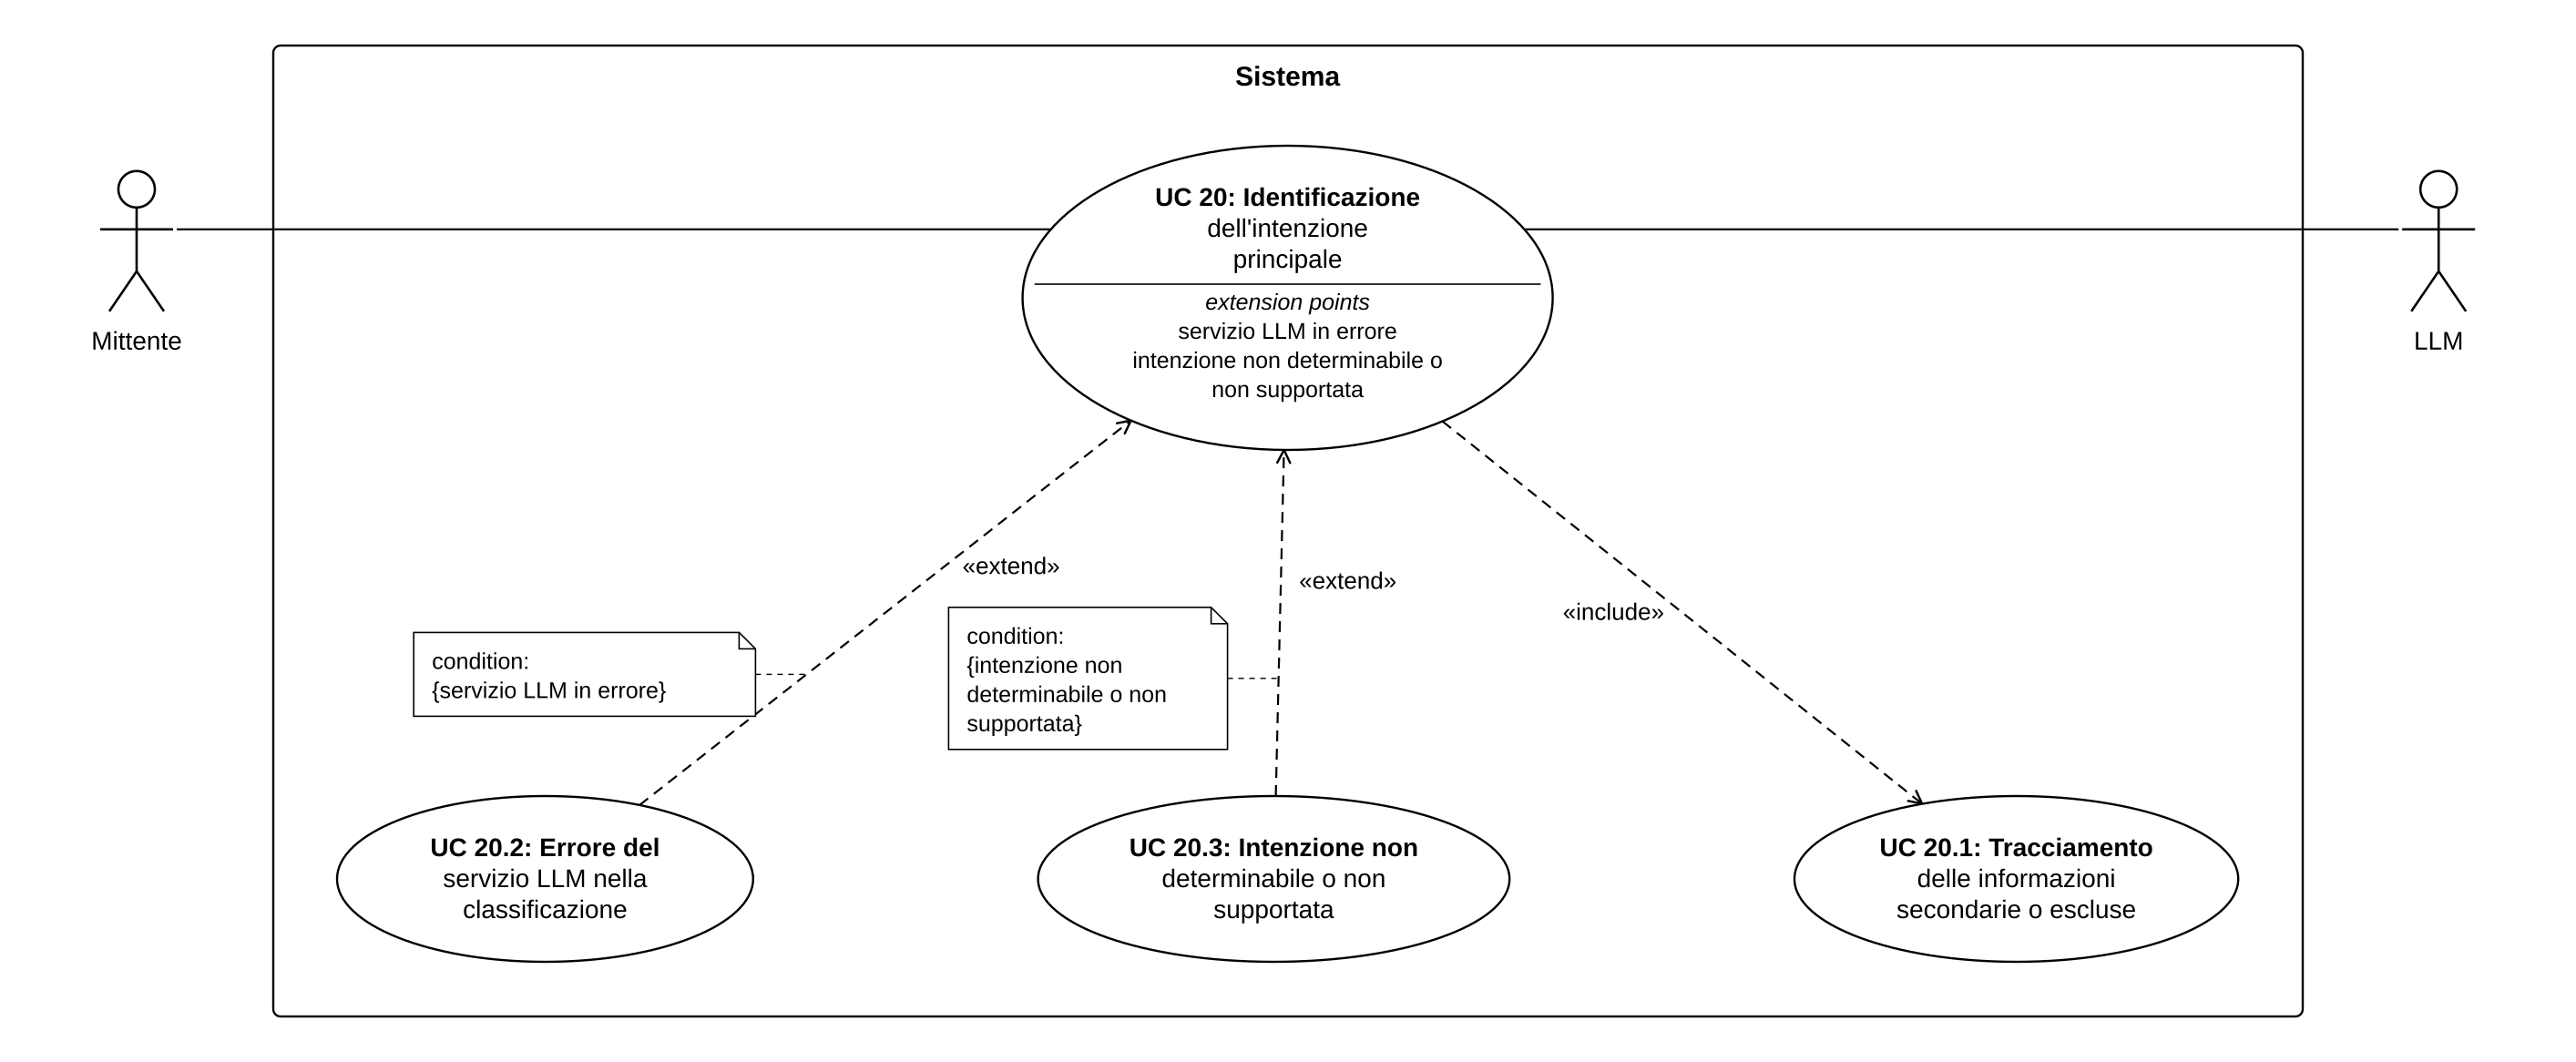
\includegraphics[width=\linewidth,height=0.32\textheight,keepaspectratio]{img/UC20.png}
\caption{UC 20 -- Identificazione dell'intenzione principale}
\end{center}
\begin{itemize}
    \item \textbf{Attore principale}: Mittente
    \item \textbf{Attori secondari}: LLM
    \item \textbf{Precondizioni}: Il testo della richiesta è disponibile e il servizio LLM è raggiungibile.
    \item \textbf{Scenario principale}:
    \begin{enumerate}
        \item Il sistema invia il contenuto all'LLM.
        \item L'LLM identifica l'intenzione principale, con priorità agli ordini d'acquisto B2B.
        \item Il sistema traccia le informazioni secondarie o escluse.
        \item Il sistema associa l'intenzione alla richiesta.
    \end{enumerate}
    \item \textbf{Postcondizioni}: L'intenzione principale è associata alla richiesta.
    \item \textbf{Trigger}: Disponibilità del contenuto estratto della richiesta.
    \item \textbf{Inclusioni}:
    \begin{itemize}
        \item \hyperref[uc:20.1]{UC 20.1}: Tracciamento delle informazioni secondarie o escluse
    \end{itemize}
    \item \textbf{Estensioni}:
    \begin{itemize}
        \item \hyperref[uc:20.2]{UC 20.2}: Errore del servizio LLM nella classificazione $\rightarrow$ Condizione: Servizio LLM in errore.
        \item \hyperref[uc:20.3]{UC 20.3}: Intenzione non determinabile o non supportata $\rightarrow$ Condizione: Intenzione non determinabile o non supportata.
    \end{itemize}
\end{itemize}

\subsubsection{UC 20.1: Tracciamento delle informazioni secondarie o escluse}\label{uc:20.1}
\begin{center}
\captionsetup{type=figure}
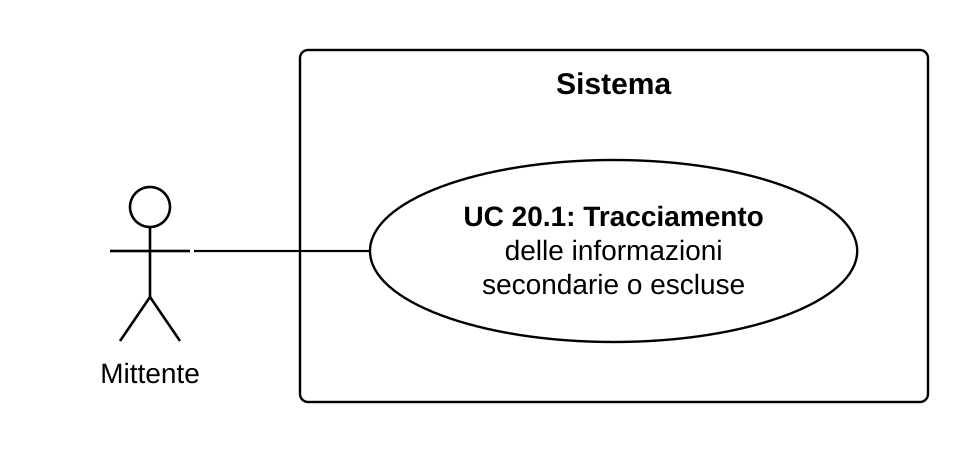
\includegraphics[width=\linewidth,height=0.32\textheight,keepaspectratio]{img/UC20_1.png}
\caption{UC 20.1 -- Tracciamento delle informazioni secondarie o escluse}
\end{center}
\begin{itemize}
    \item \textbf{Attore principale}: Mittente
    \item \textbf{Precondizioni}: L'identificazione dell'intenzione è in corso e il messaggio contiene altre informazioni.
    \item \textbf{Scenario principale}:
    \begin{enumerate}
        \item Il sistema individua le informazioni secondarie o escluse.
        \item Il sistema le registra nei log, mantenendo una sola intenzione principale.
    \end{enumerate}
    \item \textbf{Postcondizioni}: Le informazioni secondarie sono tracciate nei log.
    \item \textbf{Trigger}: Presenza di informazioni diverse dall'intenzione principale.
    \item \textbf{Incluso da}: \hyperref[uc:20]{UC 20}.
\end{itemize}

\subsubsection{UC 20.2: Errore del servizio LLM nella classificazione}\label{uc:20.2}
\begin{center}
\captionsetup{type=figure}
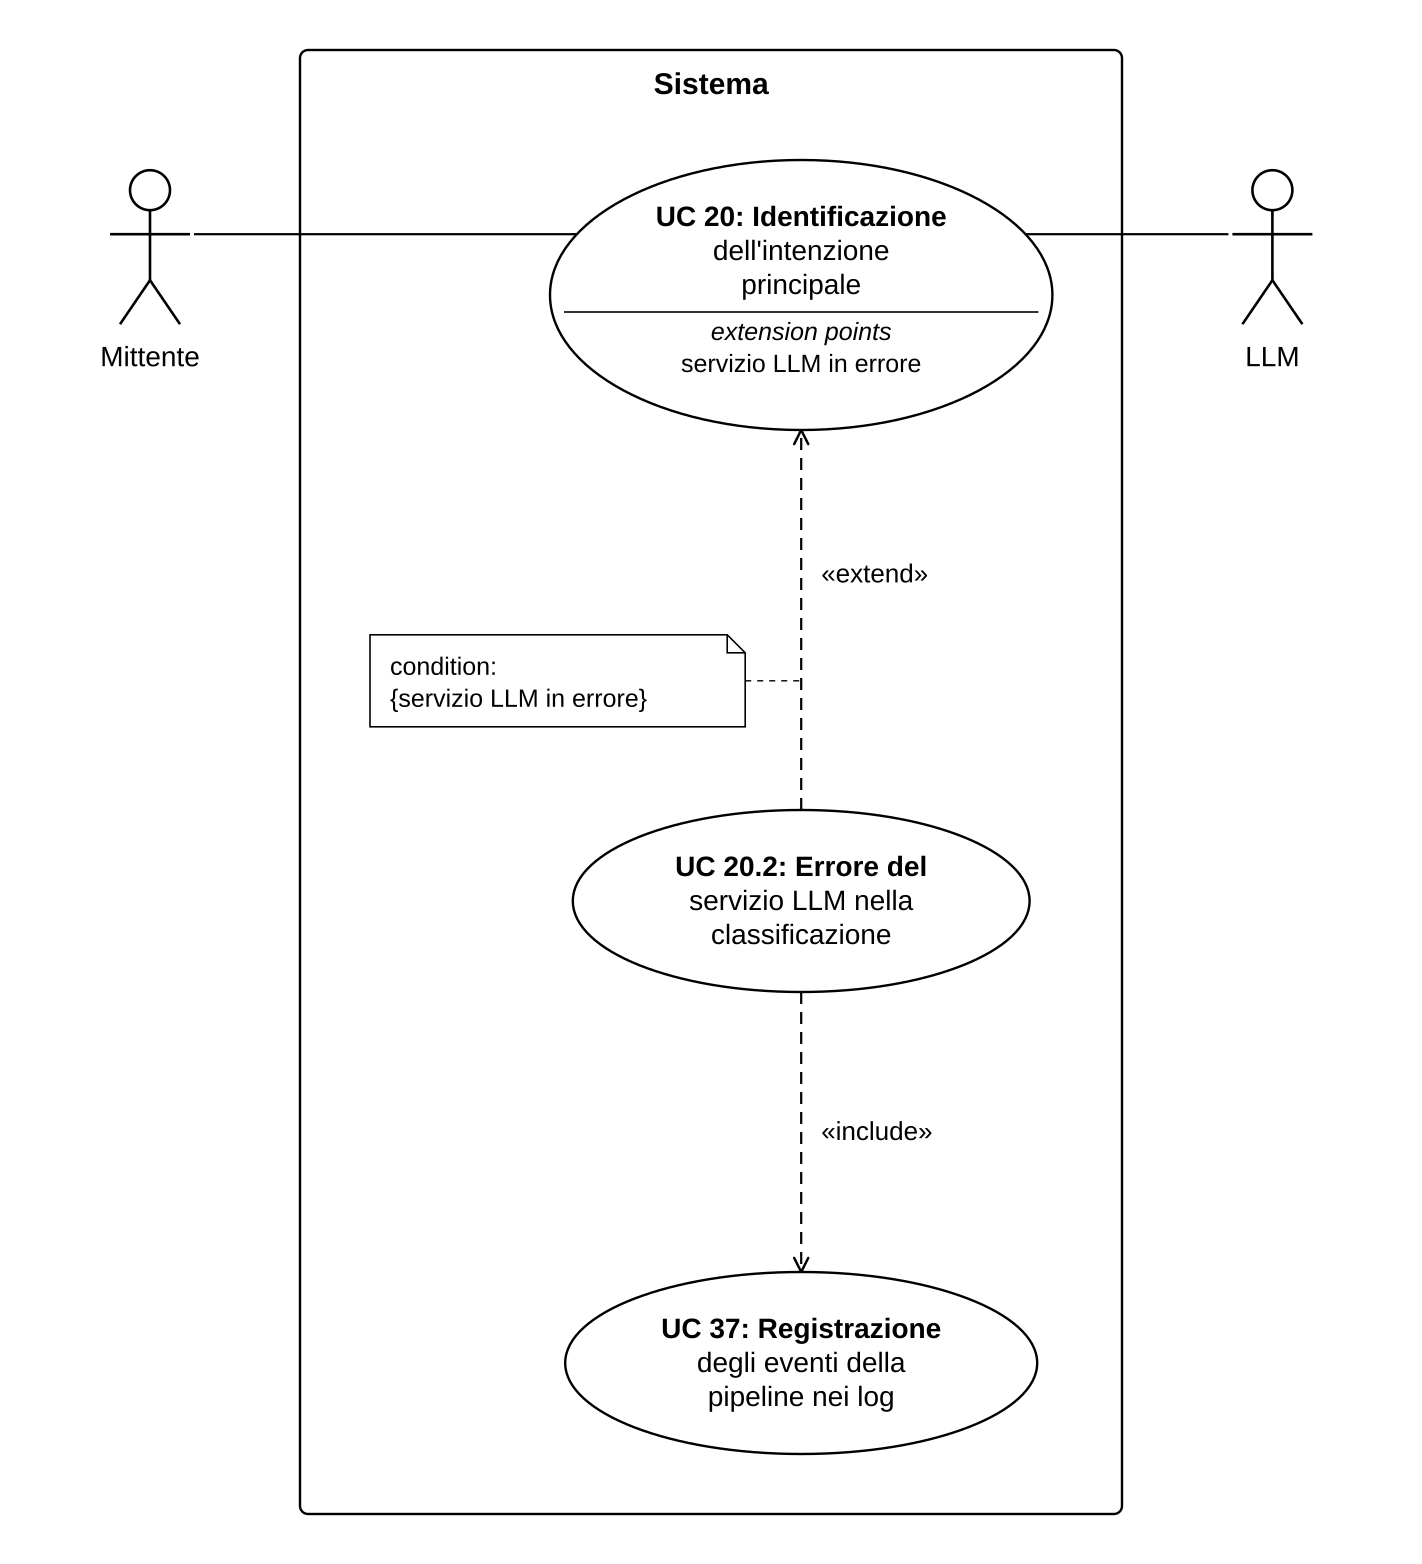
\includegraphics[width=\linewidth,height=0.32\textheight,keepaspectratio]{img/UC20_2.png}
\caption{UC 20.2 -- Errore del servizio LLM nella classificazione}
\end{center}
\begin{itemize}
    \item \textbf{Attore principale}: Mittente
    \item \textbf{Precondizioni}: La classificazione tramite LLM è in corso.
    \item \textbf{Scenario principale}:
    \begin{enumerate}
        \item Il sistema rileva un errore del servizio LLM.
        \item Il sistema registra l'errore nei log (\hyperref[uc:37]{UC 37}).
        \item Il sistema riprogramma l'elaborazione senza perdere la richiesta.
    \end{enumerate}
    \item \textbf{Postcondizioni}: L'errore è registrato e l'elaborazione è riprogrammata.
    \item \textbf{Trigger}: Errore del servizio LLM nella classificazione.
    \item \textbf{Estende}: \hyperref[uc:20]{UC 20}.
    \item \textbf{Inclusioni}:
    \begin{itemize}
        \item \hyperref[uc:37]{UC 37}: Registrazione degli eventi della pipeline nei log
    \end{itemize}
\end{itemize}

\subsubsection{UC 20.3: Intenzione non determinabile o non supportata}\label{uc:20.3}
\begin{center}
\captionsetup{type=figure}
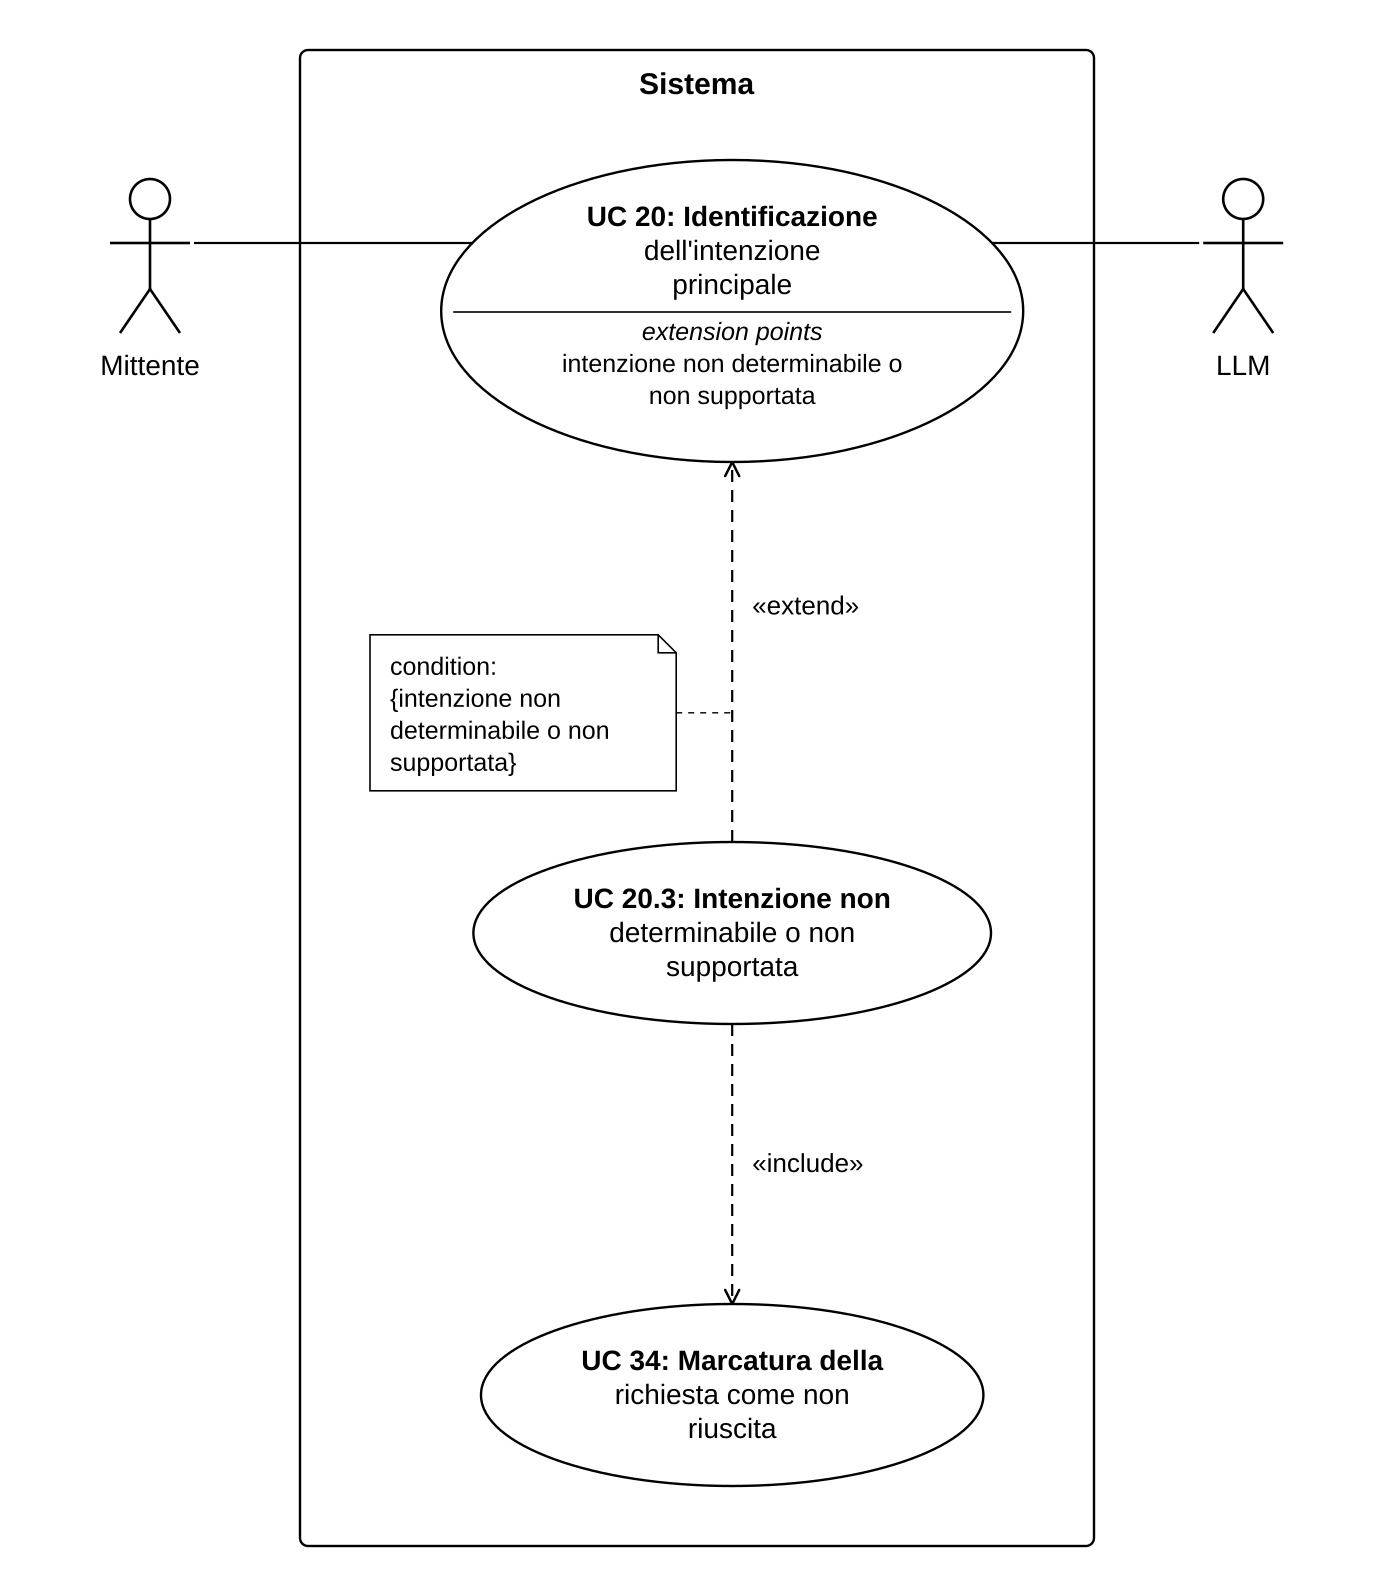
\includegraphics[width=\linewidth,height=0.32\textheight,keepaspectratio]{img/UC20_3.png}
\caption{UC 20.3 -- Intenzione non determinabile o non supportata}
\end{center}
\begin{itemize}
    \item \textbf{Attore principale}: Mittente
    \item \textbf{Precondizioni}: L'identificazione dell'intenzione è in corso.
    \item \textbf{Scenario principale}:
    \begin{enumerate}
        \item Il sistema rileva che l'intenzione principale non è determinabile o non è supportata.
        \item Il sistema marca la richiesta come non riuscita (\hyperref[uc:34]{UC 34}).
        \item Il sistema registra l'evento nei log (\hyperref[uc:37]{UC 37}).
    \end{enumerate}
    \item \textbf{Postcondizioni}: La richiesta è marcata come non riuscita e l'evento è registrato nei log.
    \item \textbf{Trigger}: Intenzione non determinabile o non supportata.
    \item \textbf{Estende}: \hyperref[uc:20]{UC 20}.
    \item \textbf{Inclusioni}:
    \begin{itemize}
        \item \hyperref[uc:34]{UC 34}: Marcatura della richiesta come non riuscita
    \end{itemize}
\end{itemize}

\subsubsection{UC 21: Estrazione delle entità dell'ordine d'acquisto}\label{uc:21}
\begin{center}
\captionsetup{type=figure}
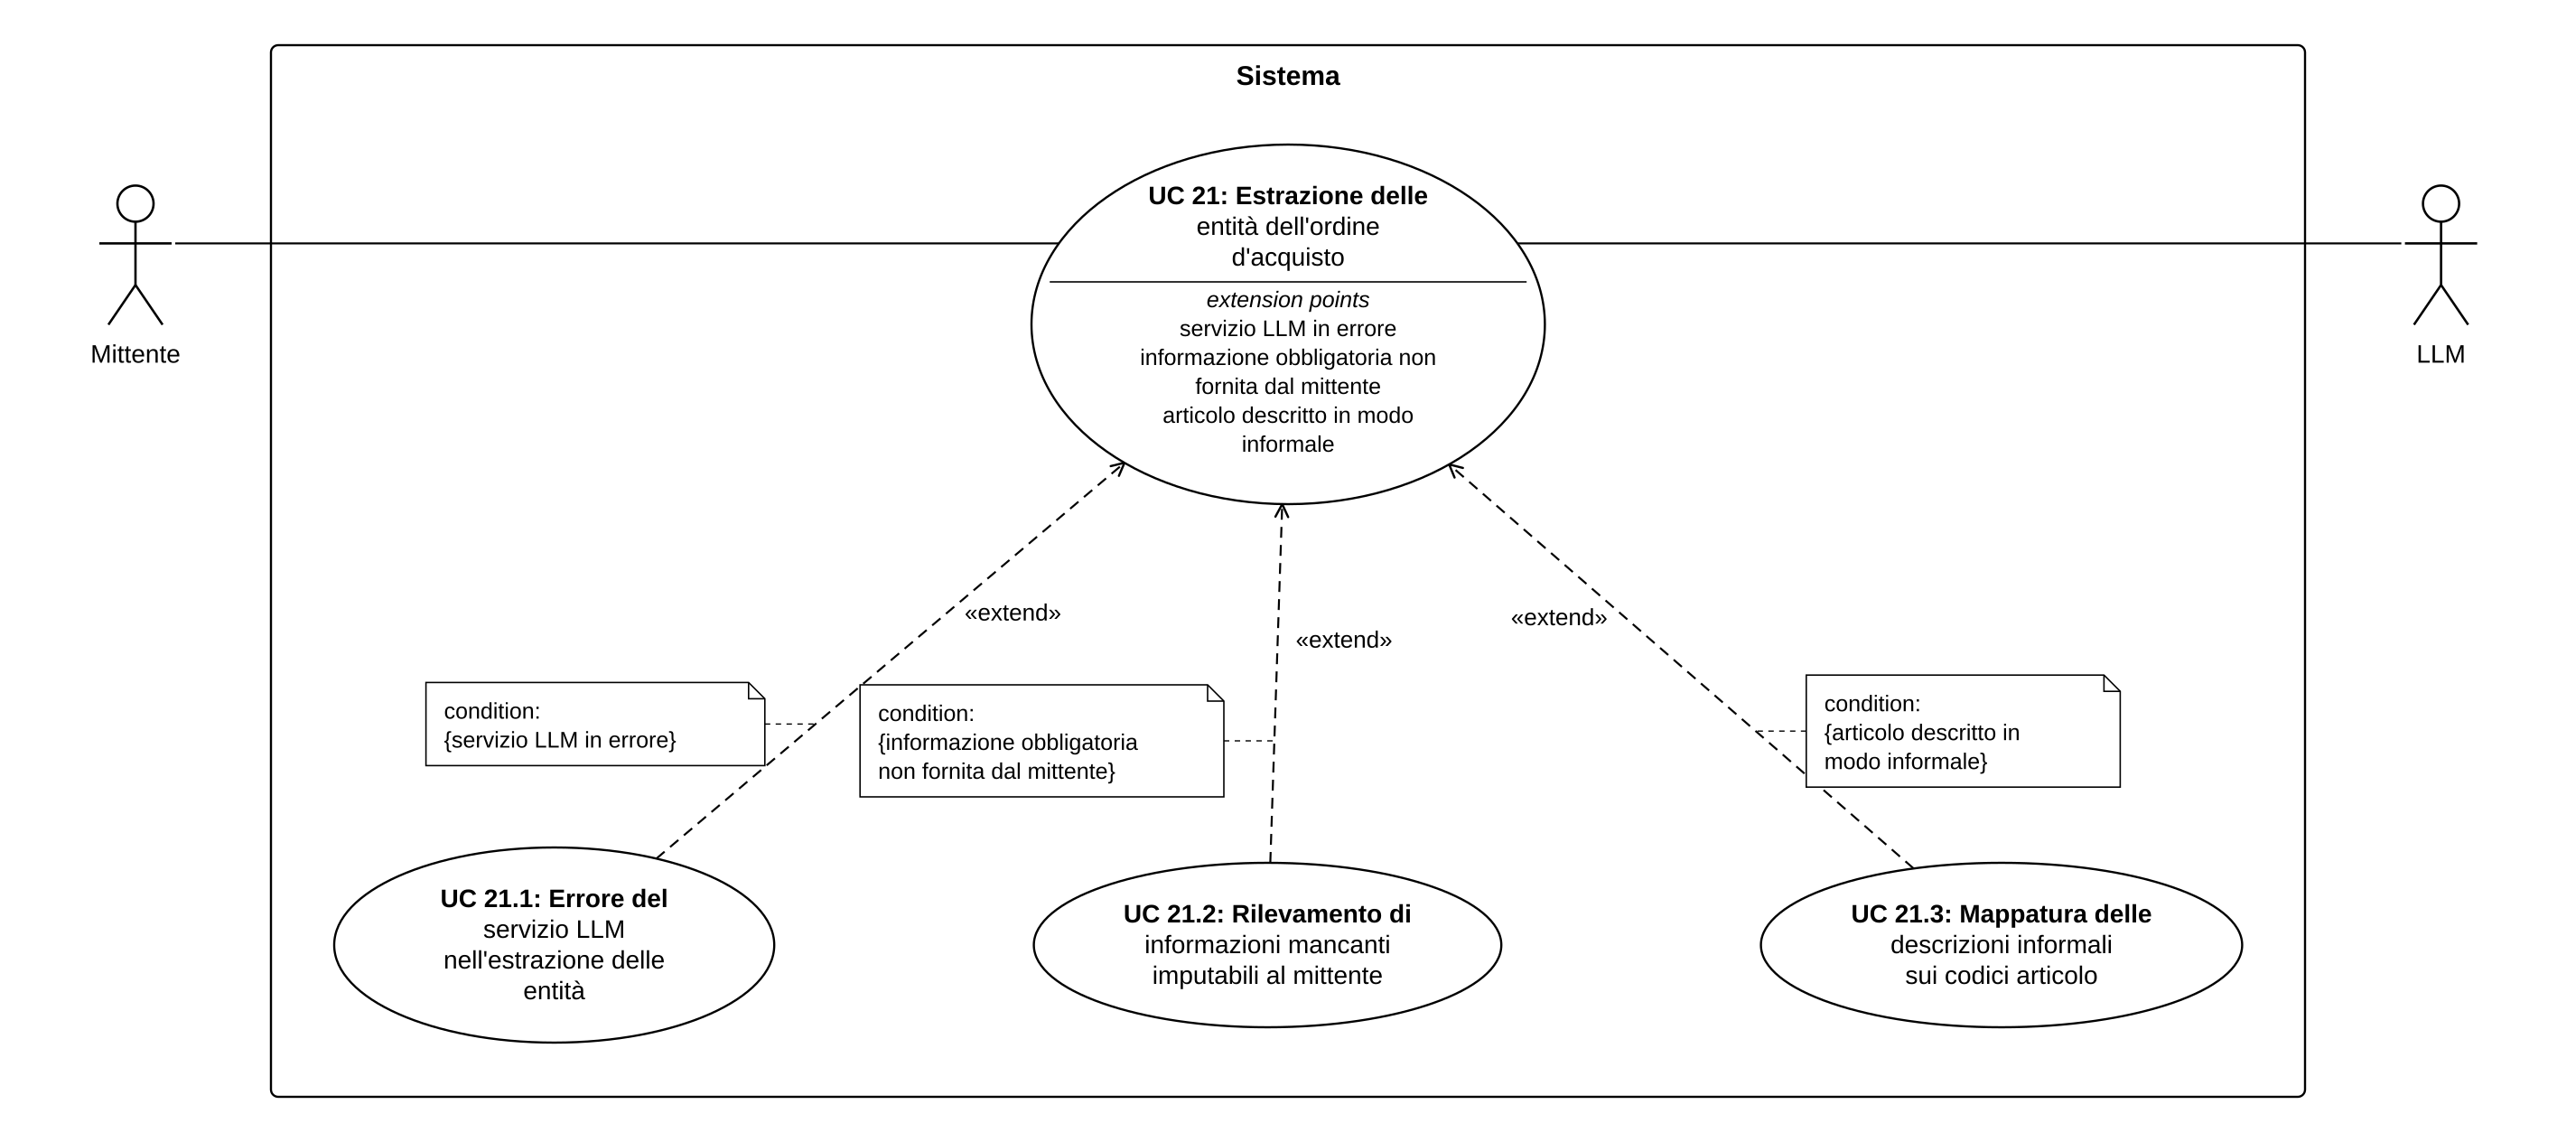
\includegraphics[width=\linewidth,height=0.32\textheight,keepaspectratio]{img/UC21.png}
\caption{UC 21 -- Estrazione delle entità dell'ordine d'acquisto}
\end{center}
\begin{itemize}
    \item \textbf{Attore principale}: Mittente
    \item \textbf{Attori secondari}: LLM
    \item \textbf{Precondizioni}: L'intenzione identificata è un ordine d'acquisto e il servizio LLM è raggiungibile.
    \item \textbf{Scenario principale}:
    \begin{enumerate}
        \item Il sistema invia il contenuto all'LLM.
        \item L'LLM estrae codici articolo, quantità, dati cliente e dati di spedizione.
        \item Il sistema associa le entità alla richiesta.
    \end{enumerate}
    \item \textbf{Postcondizioni}: Le entità dell'ordine sono associate alla richiesta.
    \item \textbf{Trigger}: Identificazione di un ordine d'acquisto.
    \item \textbf{Estensioni}:
    \begin{itemize}
        \item \hyperref[uc:21.1]{UC 21.1}: Errore del servizio LLM nell'estrazione delle entità $\rightarrow$ Condizione: Servizio LLM in errore.
        \item \hyperref[uc:21.2]{UC 21.2}: Rilevamento di informazioni mancanti imputabili al mittente $\rightarrow$ Condizione: Informazione obbligatoria non fornita dal mittente.
        \item \hyperref[uc:21.3]{UC 21.3}: Mappatura delle descrizioni informali sui codici articolo $\rightarrow$ Condizione: Articolo descritto in modo informale.
    \end{itemize}
\end{itemize}

\subsubsection{UC 21.1: Errore del servizio LLM nell'estrazione delle entità}\label{uc:21.1}
\begin{center}
\captionsetup{type=figure}
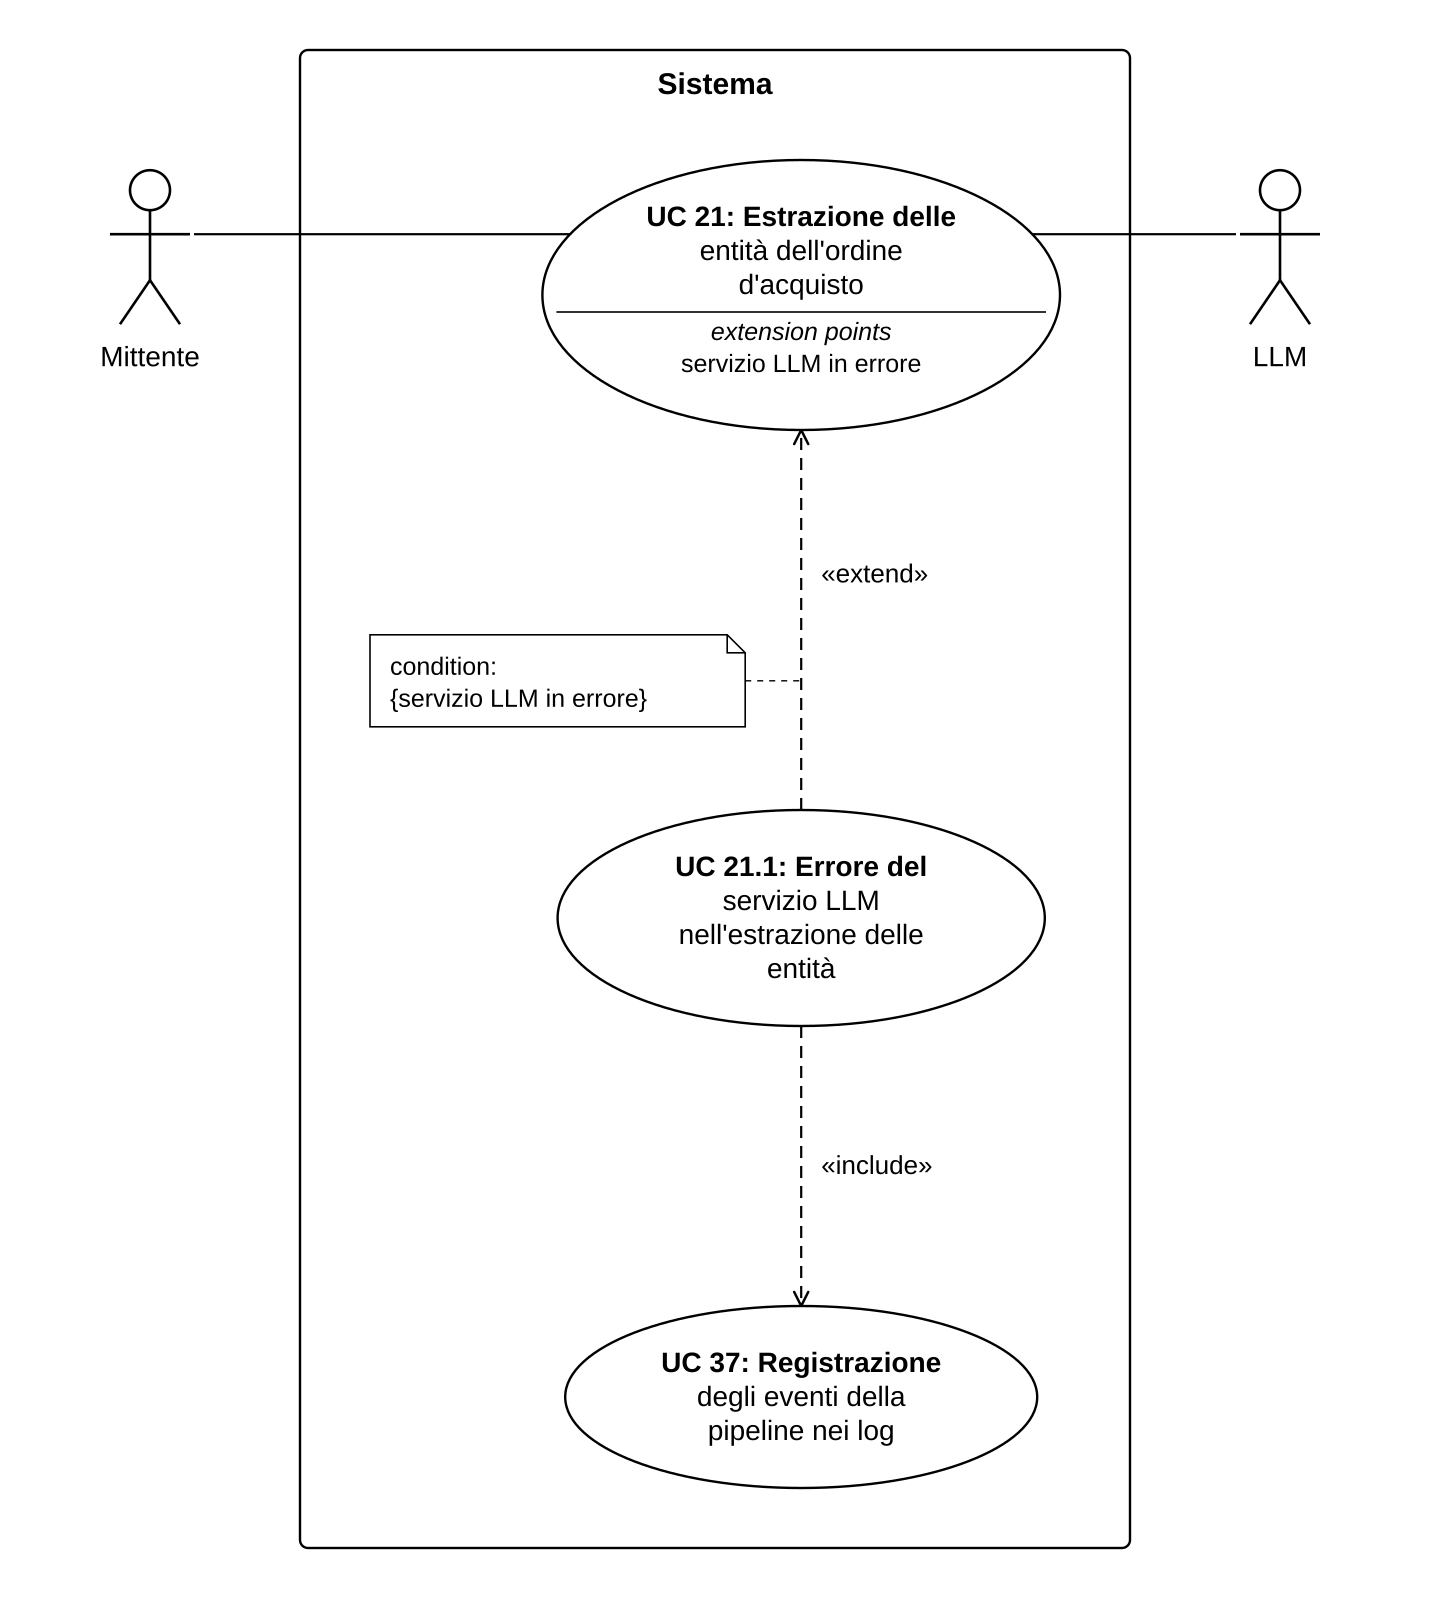
\includegraphics[width=\linewidth,height=0.32\textheight,keepaspectratio]{img/UC21_1.png}
\caption{UC 21.1 -- Errore del servizio LLM nell'estrazione delle entità}
\end{center}
\begin{itemize}
    \item \textbf{Attore principale}: Mittente
    \item \textbf{Precondizioni}: L'estrazione delle entità è in corso.
    \item \textbf{Scenario principale}:
    \begin{enumerate}
        \item Il sistema rileva un errore del servizio LLM.
        \item Il sistema registra l'errore nei log (\hyperref[uc:37]{UC 37}).
        \item Il sistema riprogramma l'elaborazione senza perdere la richiesta.
    \end{enumerate}
    \item \textbf{Postcondizioni}: L'errore è registrato e l'elaborazione è riprogrammata.
    \item \textbf{Trigger}: Errore del servizio LLM nell'estrazione delle entità.
    \item \textbf{Estende}: \hyperref[uc:21]{UC 21}.
    \item \textbf{Inclusioni}:
    \begin{itemize}
        \item \hyperref[uc:37]{UC 37}: Registrazione degli eventi della pipeline nei log
    \end{itemize}
\end{itemize}

\subsubsection{UC 21.2: Rilevamento di informazioni mancanti imputabili al mittente}\label{uc:21.2}
\begin{center}
\captionsetup{type=figure}
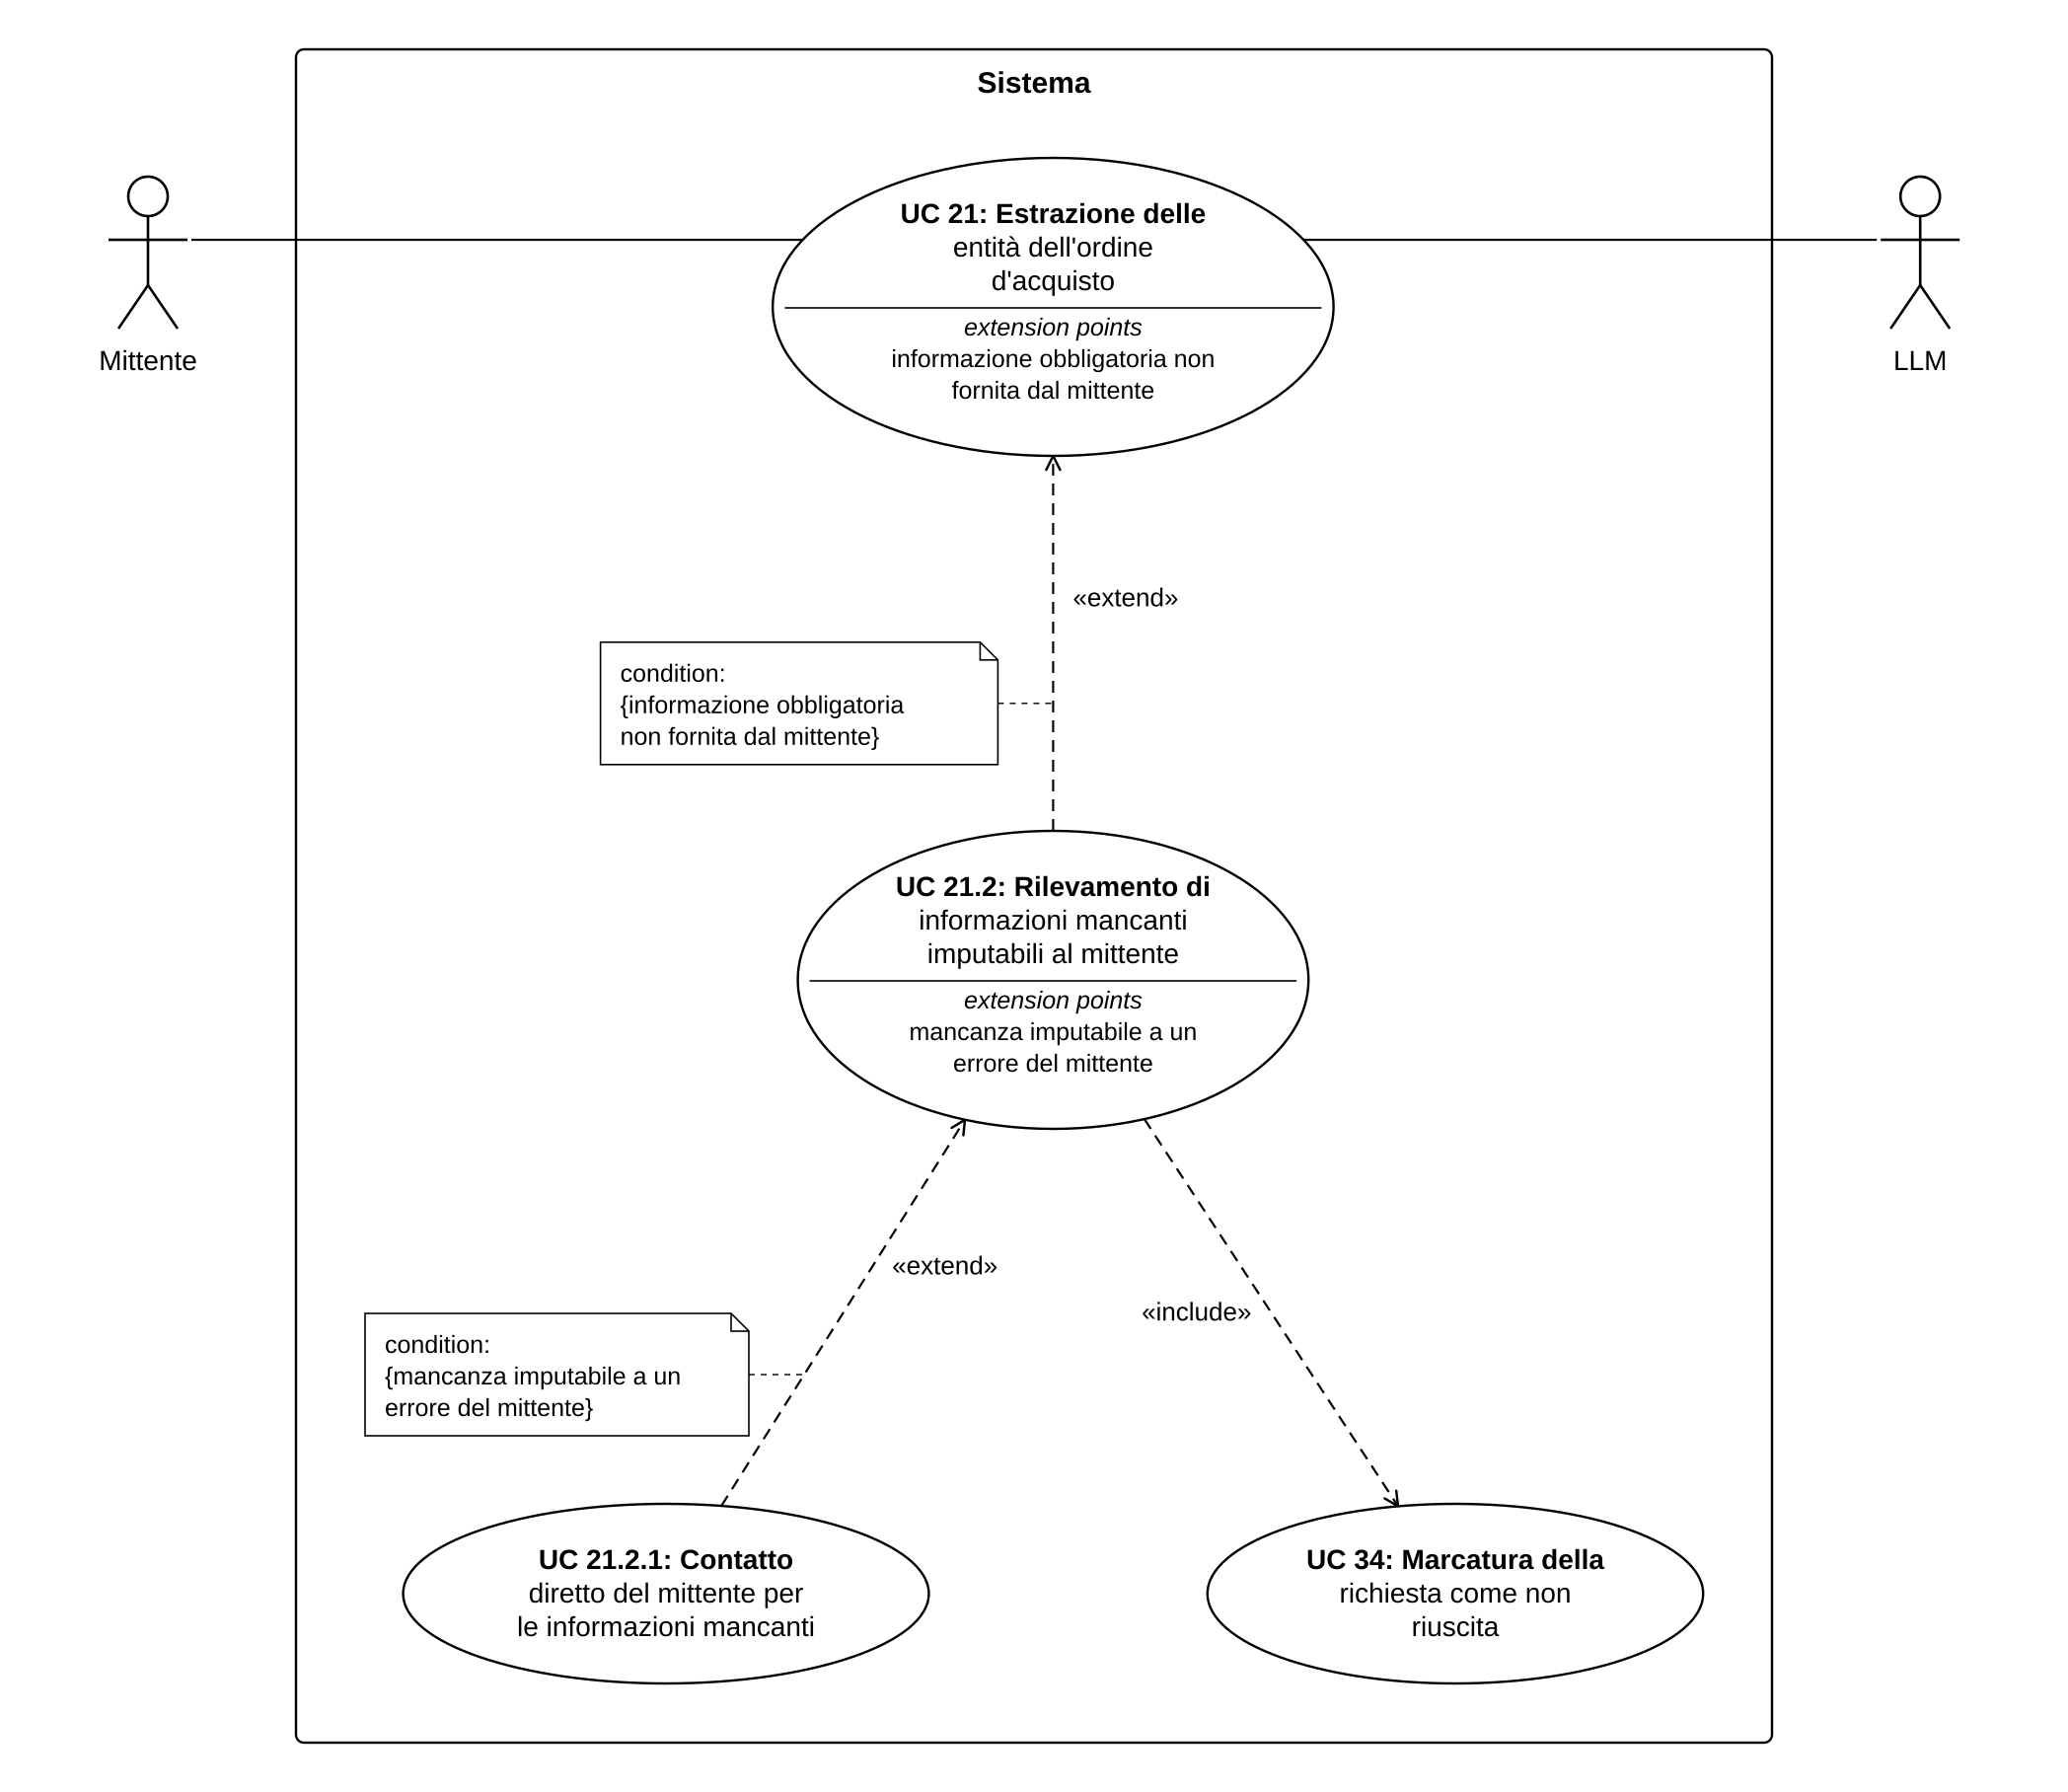
\includegraphics[width=\linewidth,height=0.32\textheight,keepaspectratio]{img/UC21_2.png}
\caption{UC 21.2 -- Rilevamento di informazioni mancanti imputabili al mittente}
\end{center}
\begin{itemize}
    \item \textbf{Attore principale}: Mittente
    \item \textbf{Precondizioni}: L'estrazione delle entità è in corso.
    \item \textbf{Scenario principale}:
    \begin{enumerate}
        \item Il sistema rileva informazioni mancanti imputabili al mittente, ad esempio la quantità non specificata.
        \item Il sistema marca la richiesta come non riuscita (\hyperref[uc:34]{UC 34}).
        \item Il sistema non inoltra automaticamente la richiesta.
    \end{enumerate}
    \item \textbf{Postcondizioni}: La richiesta è marcata come non riuscita e non è inoltrata.
    \item \textbf{Trigger}: Informazione obbligatoria non fornita dal mittente.
    \item \textbf{Estende}: \hyperref[uc:21]{UC 21}.
    \item \textbf{Inclusioni}:
    \begin{itemize}
        \item \hyperref[uc:34]{UC 34}: Marcatura della richiesta come non riuscita
    \end{itemize}
    \item \textbf{Estensioni}:
    \begin{itemize}
        \item \hyperref[uc:21.2.1]{UC 21.2.1}: Contatto diretto del mittente per le informazioni mancanti $\rightarrow$ Condizione: Mancanza imputabile a un errore del mittente.
    \end{itemize}
\end{itemize}

\subsubsection{UC 21.2.1: Contatto diretto del mittente per le informazioni mancanti}\label{uc:21.2.1}
\begin{center}
\captionsetup{type=figure}
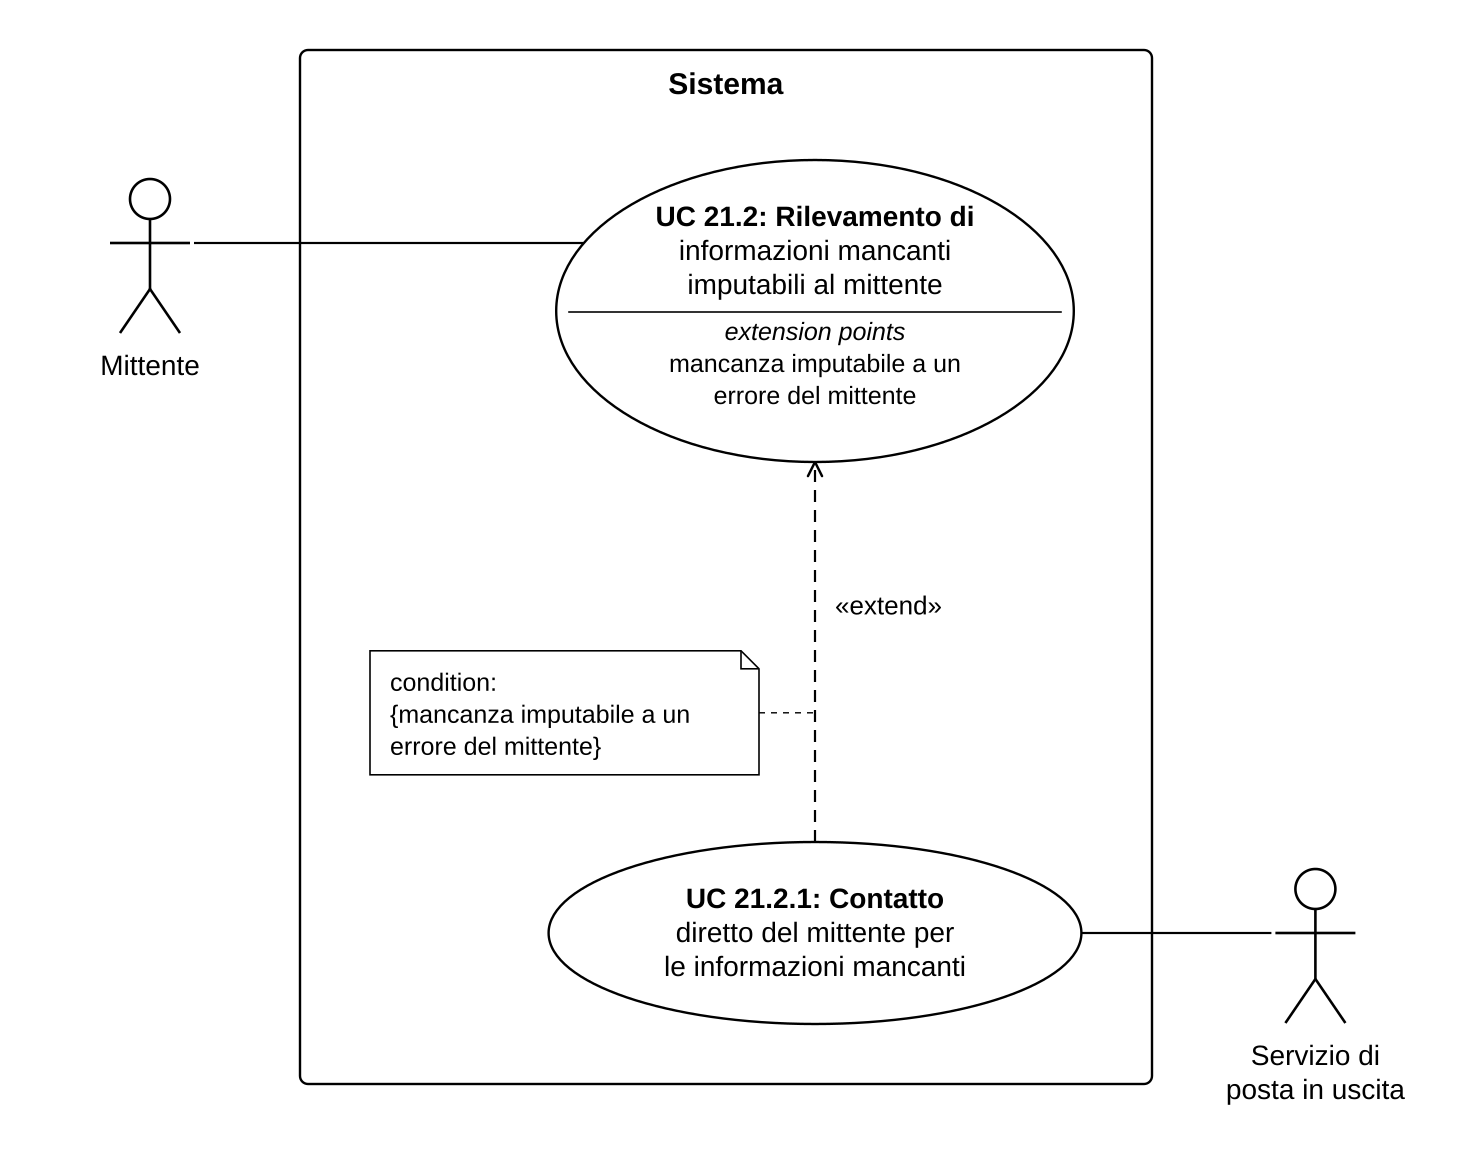
\includegraphics[width=\linewidth,height=0.32\textheight,keepaspectratio]{img/UC21_2_1.png}
\caption{UC 21.2.1 -- Contatto diretto del mittente per le informazioni mancanti}
\end{center}
\begin{itemize}
    \item \textbf{Attore principale}: Mittente
    \item \textbf{Attori secondari}: Servizio di posta in uscita
    \item \textbf{Precondizioni}: Il rilevamento di informazioni mancanti ha individuato un errore imputabile al mittente.
    \item \textbf{Scenario principale}:
    \begin{enumerate}
        \item Il sistema compone un messaggio con le informazioni mancanti.
        \item Il sistema invia l'e-mail al mittente tramite il servizio di posta in uscita.
    \end{enumerate}
    \item \textbf{Postcondizioni}: Il mittente è stato contattato per completare la richiesta.
    \item \textbf{Trigger}: Mancanza di informazioni imputabile al mittente.
    \item \textbf{Estende}: \hyperref[uc:21.2]{UC 21.2}.
\end{itemize}

\subsubsection{UC 21.3: Mappatura delle descrizioni informali sui codici articolo}\label{uc:21.3}
\begin{center}
\captionsetup{type=figure}
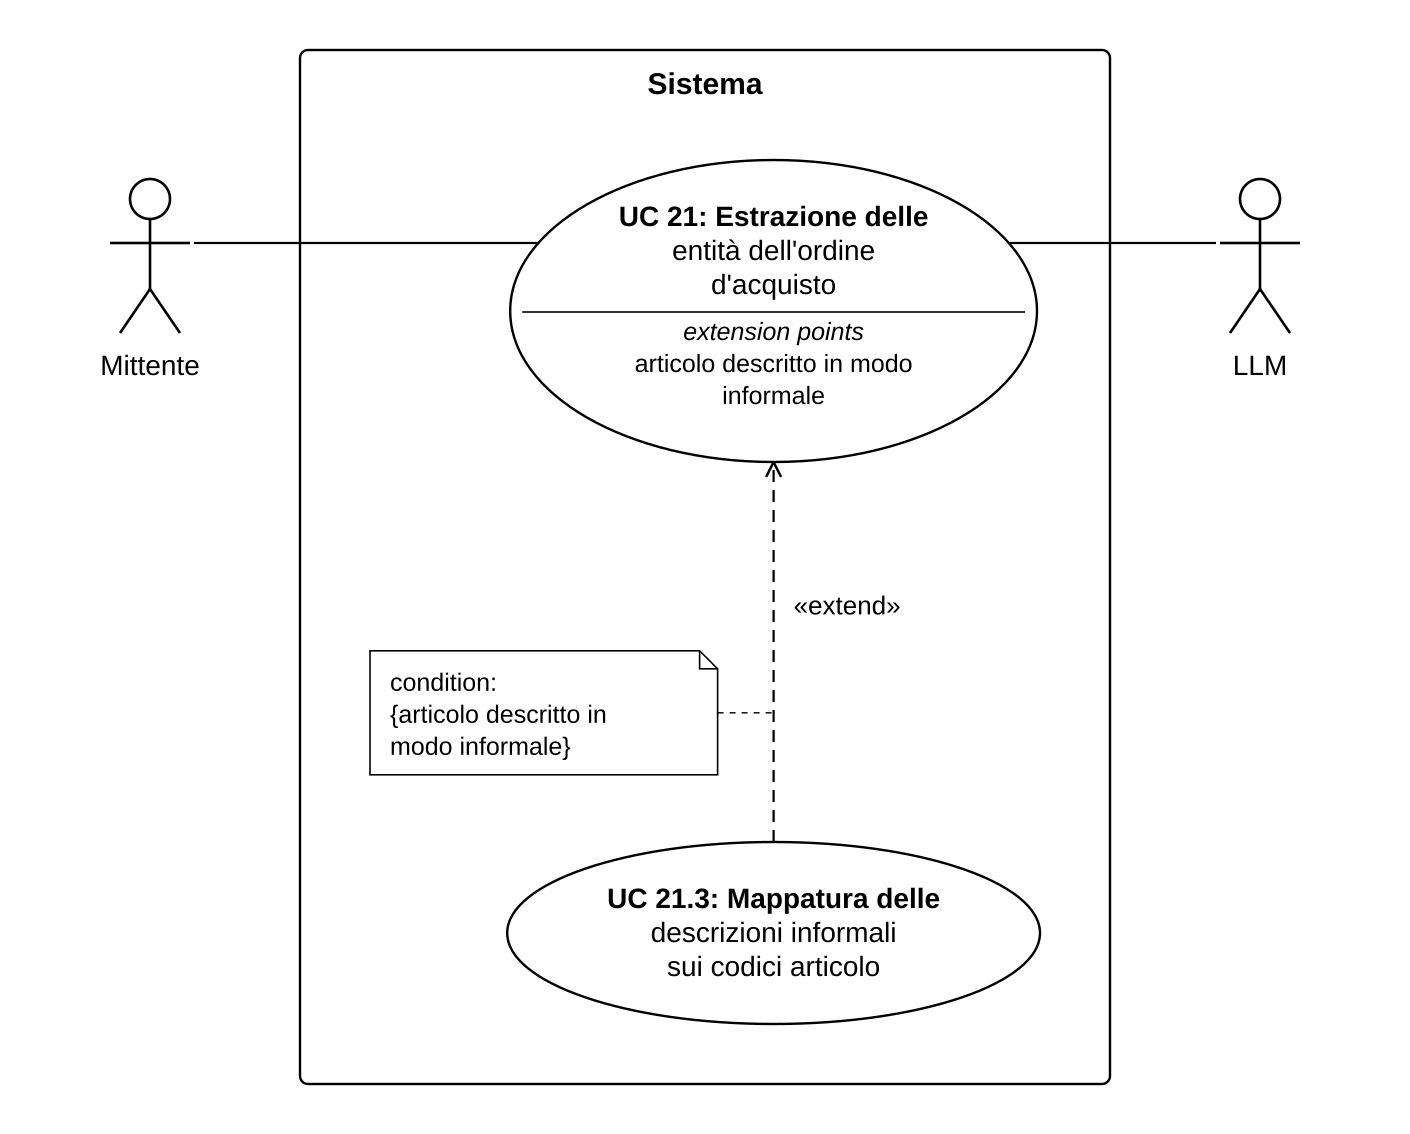
\includegraphics[width=\linewidth,height=0.32\textheight,keepaspectratio]{img/UC21_3.png}
\caption{UC 21.3 -- Mappatura delle descrizioni informali sui codici articolo}
\end{center}
\begin{itemize}
    \item \textbf{Attore principale}: Mittente
    \item \textbf{Attori secondari}: LLM
    \item \textbf{Precondizioni}: L'estrazione delle entità è in corso e un articolo è descritto in modo informale.
    \item \textbf{Scenario principale}:
    \begin{enumerate}
        \item Il sistema invia la descrizione dell'articolo all'LLM.
        \item L'LLM la mappa su un codice articolo del catalogo.
        \item Il sistema associa il codice alla richiesta senza verificarne l'esistenza.
    \end{enumerate}
    \item \textbf{Postcondizioni}: La descrizione informale è associata a un codice articolo.
    \item \textbf{Trigger}: Presenza di un articolo descritto in modo informale.
    \item \textbf{Estende}: \hyperref[uc:21]{UC 21}.
\end{itemize}

\subsubsection{UC 22: Strutturazione dei dati dell'ordine in template JSON}\label{uc:22}
\begin{center}
\captionsetup{type=figure}
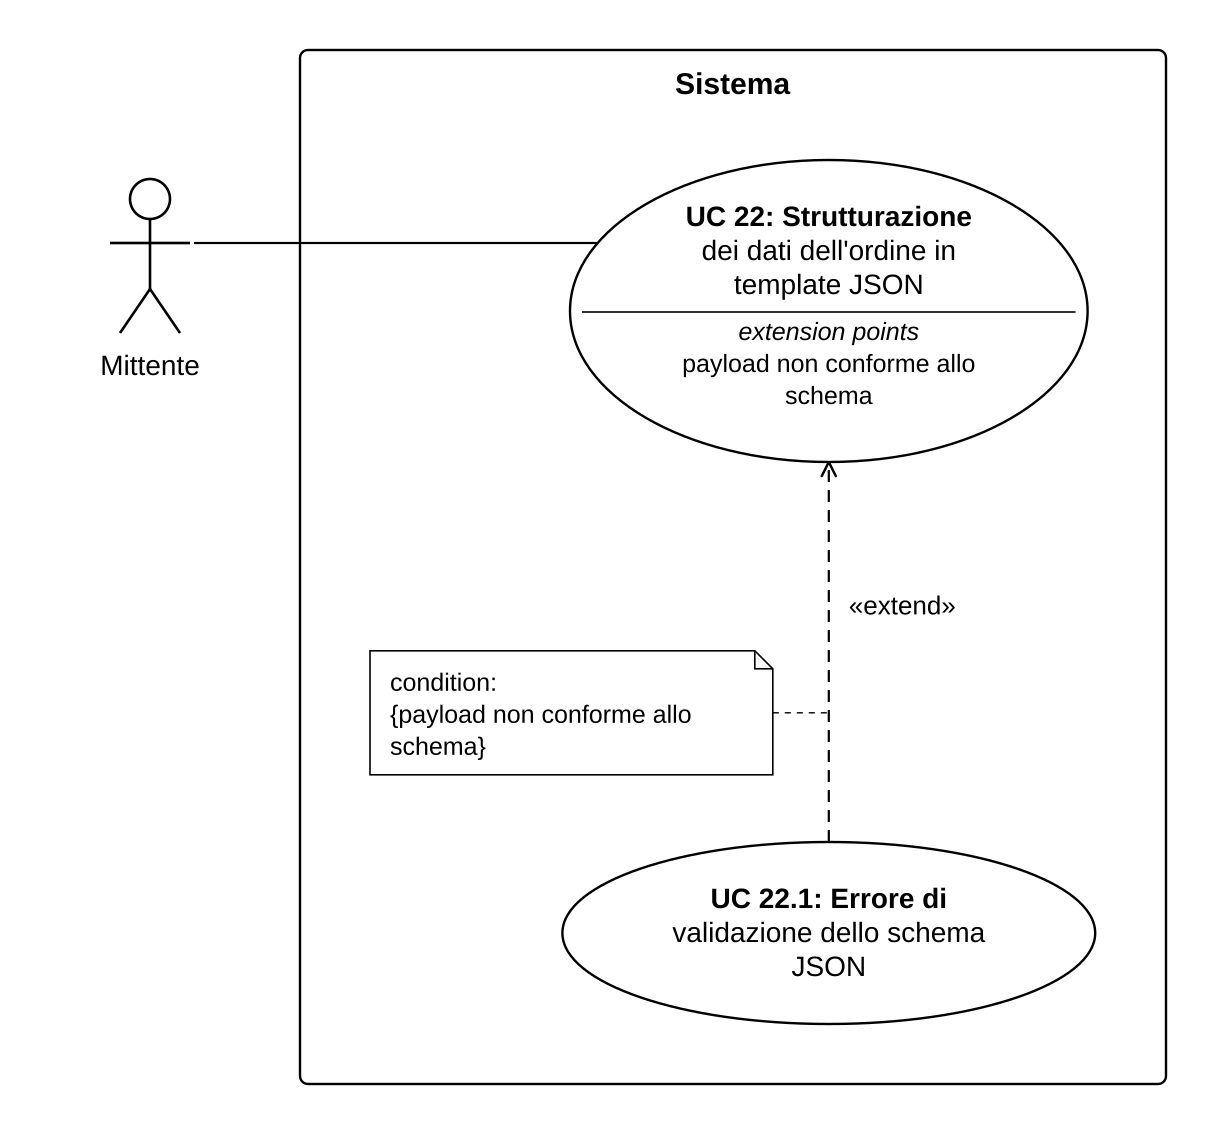
\includegraphics[width=\linewidth,height=0.32\textheight,keepaspectratio]{img/UC22.png}
\caption{UC 22 -- Strutturazione dei dati dell'ordine in template JSON}
\end{center}
\begin{itemize}
    \item \textbf{Attore principale}: Mittente
    \item \textbf{Precondizioni}: Le entità dell'ordine sono state estratte.
    \item \textbf{Scenario principale}:
    \begin{enumerate}
        \item Il sistema organizza i dati dell'ordine nel template JSON.
        \item Il sistema valida il payload rispetto allo schema.
        \item Il sistema associa il payload alla richiesta.
    \end{enumerate}
    \item \textbf{Postcondizioni}: Il payload JSON valido è associato alla richiesta.
    \item \textbf{Trigger}: Completamento dell'estrazione delle entità.
    \item \textbf{Estensioni}:
    \begin{itemize}
        \item \hyperref[uc:22.1]{UC 22.1}: Errore di validazione dello schema JSON $\rightarrow$ Condizione: Payload non conforme allo schema.
    \end{itemize}
\end{itemize}

\subsubsection{UC 22.1: Errore di validazione dello schema JSON}\label{uc:22.1}
\begin{center}
\captionsetup{type=figure}
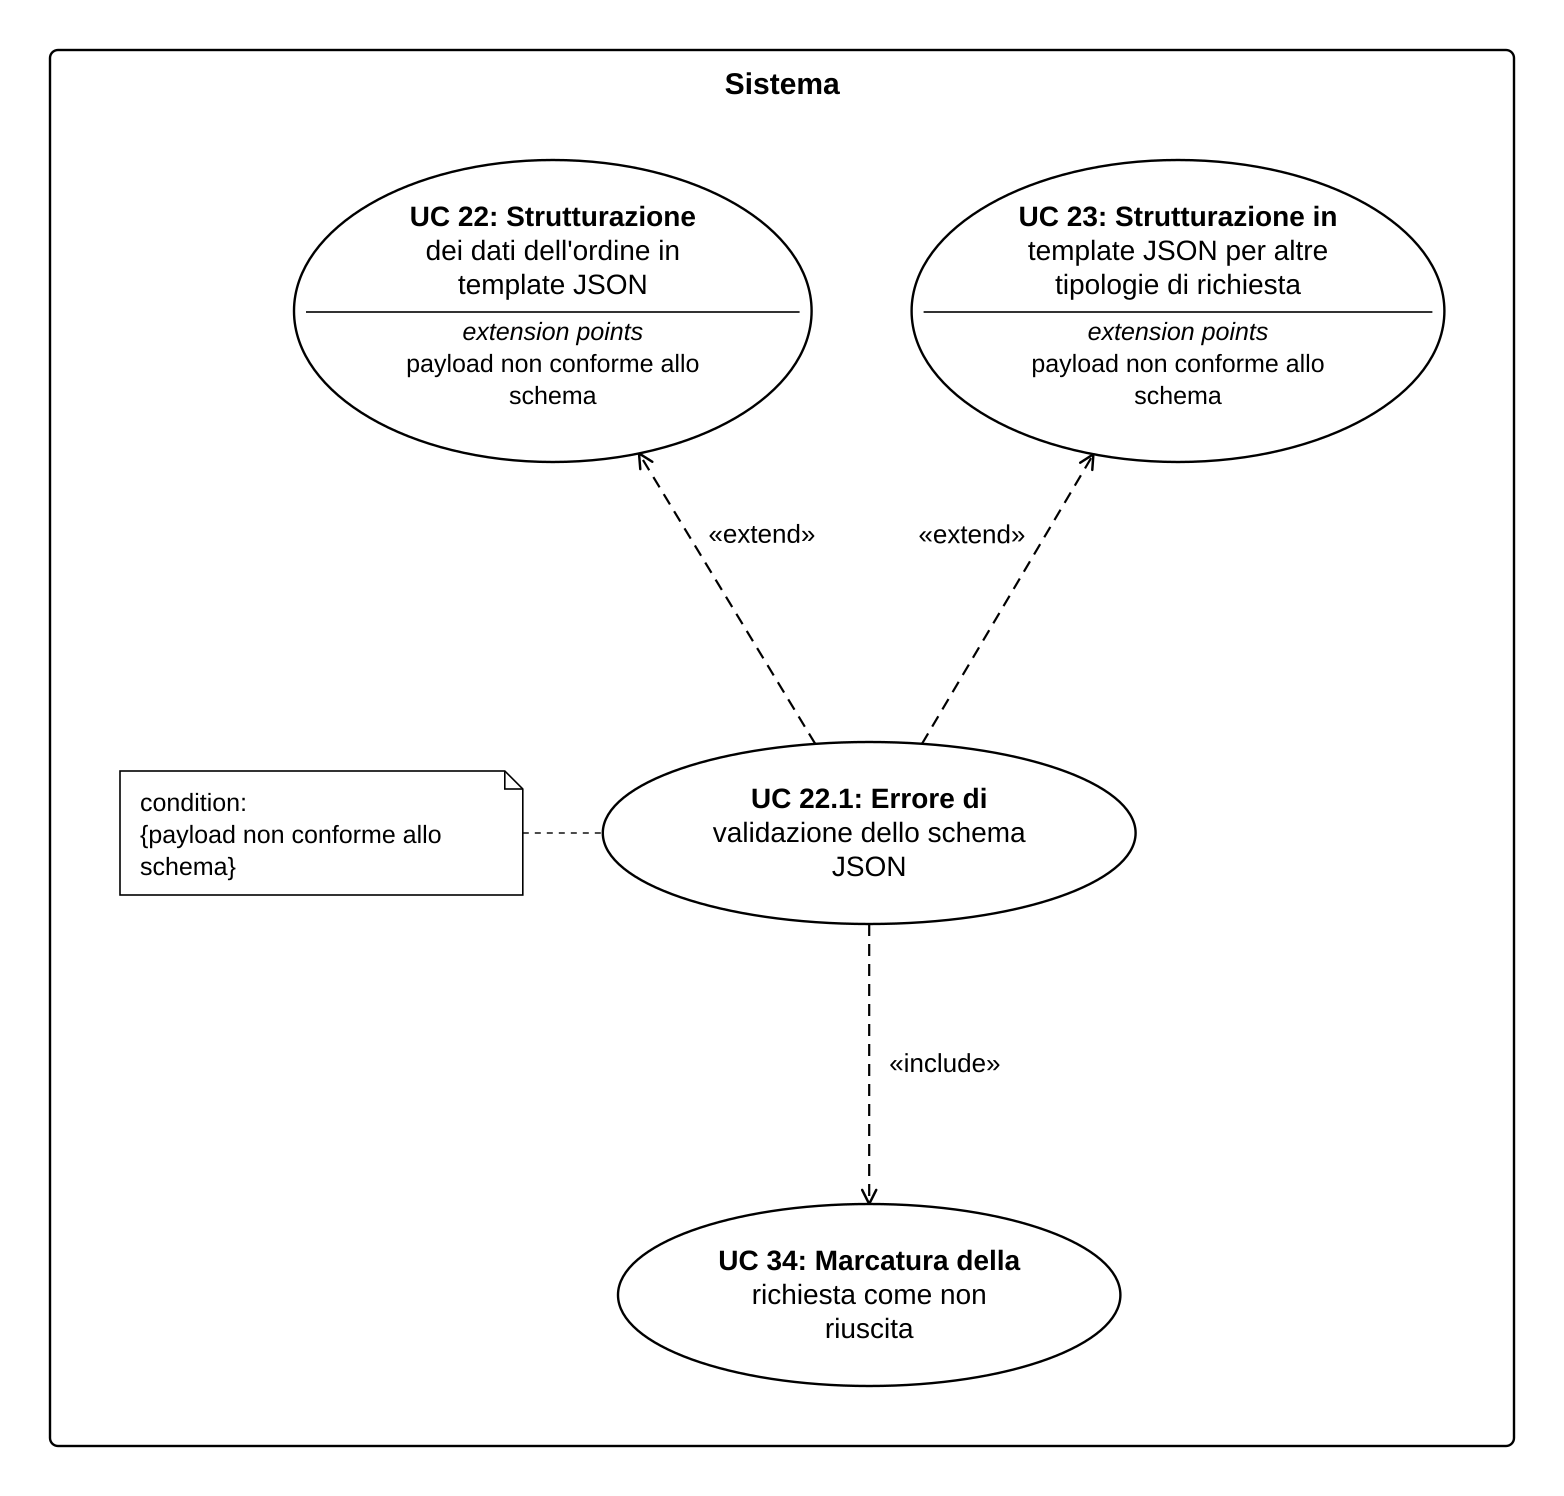
\includegraphics[width=\linewidth,height=0.32\textheight,keepaspectratio]{img/UC22_1.png}
\caption{UC 22.1 -- Errore di validazione dello schema JSON}
\end{center}
\begin{itemize}
    \item \textbf{Attore principale}: Mittente
    \item \textbf{Precondizioni}: La validazione del payload è in corso.
    \item \textbf{Scenario principale}:
    \begin{enumerate}
        \item Il sistema rileva che il payload non supera la validazione dello schema.
        \item Il sistema marca la richiesta come non riuscita (\hyperref[uc:34]{UC 34}).
        \item Il sistema registra nei log i campi non conformi (\hyperref[uc:37]{UC 37}).
    \end{enumerate}
    \item \textbf{Postcondizioni}: La richiesta è marcata come non riuscita e i campi non conformi sono registrati nei log.
    \item \textbf{Trigger}: Payload non conforme allo schema.
    \item \textbf{Estende}: \hyperref[uc:22]{UC 22}, \hyperref[uc:23]{UC 23}.
    \item \textbf{Inclusioni}:
    \begin{itemize}
        \item \hyperref[uc:34]{UC 34}: Marcatura della richiesta come non riuscita
    \end{itemize}
\end{itemize}

\subsubsection{UC 23: Strutturazione in template JSON per altre tipologie di richiesta}\label{uc:23}
\begin{center}
\captionsetup{type=figure}
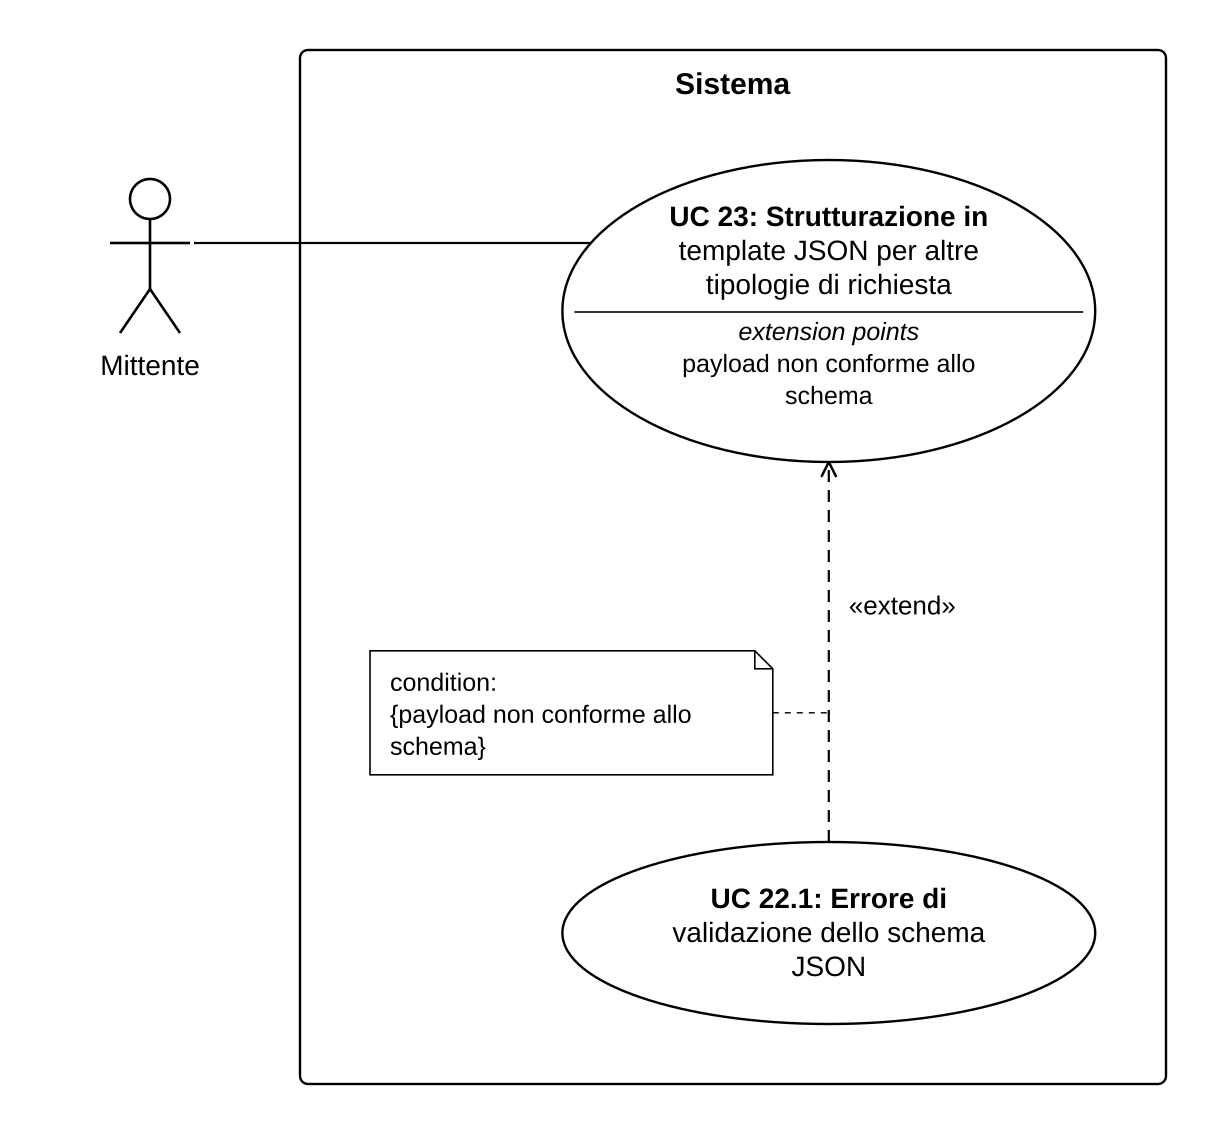
\includegraphics[width=\linewidth,height=0.32\textheight,keepaspectratio]{img/UC23.png}
\caption{UC 23 -- Strutturazione in template JSON per altre tipologie di richiesta}
\end{center}
\begin{itemize}
    \item \textbf{Attore principale}: Mittente
    \item \textbf{Precondizioni}: È stata identificata una richiesta diversa da un ordine d'acquisto.
    \item \textbf{Scenario principale}:
    \begin{enumerate}
        \item Il sistema seleziona il template JSON per la tipologia della richiesta.
        \item Il sistema organizza i dati nel template e li valida.
        \item Il sistema associa il payload alla richiesta.
    \end{enumerate}
    \item \textbf{Postcondizioni}: Il payload JSON è associato alla richiesta.
    \item \textbf{Trigger}: Identificazione di una richiesta di assistenza, appuntamento, opportunità o documento contabile.
    \item \textbf{Estensioni}:
    \begin{itemize}
        \item \hyperref[uc:22.1]{UC 22.1}: Errore di validazione dello schema JSON $\rightarrow$ Condizione: Payload non conforme allo schema.
    \end{itemize}
\end{itemize}

\subsubsection{UC 24: Applicazione della priorità al testo del messaggio}\label{uc:24}
\begin{center}
\captionsetup{type=figure}
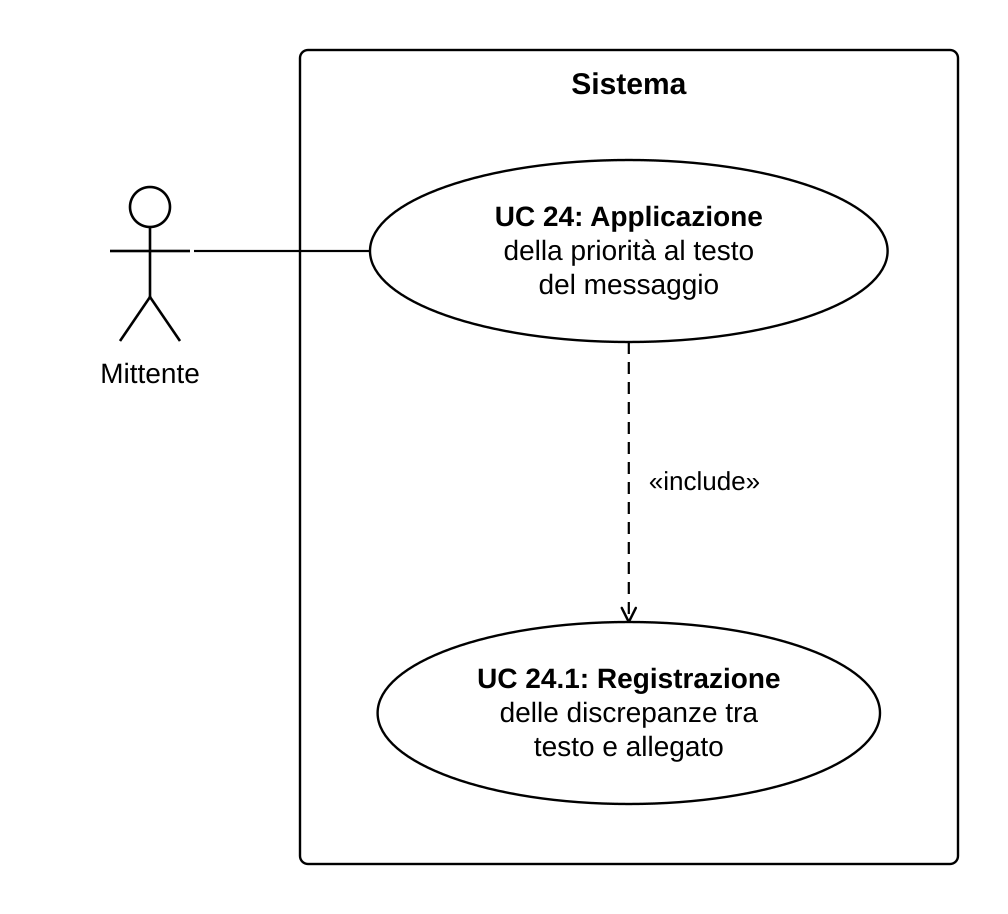
\includegraphics[width=\linewidth,height=0.32\textheight,keepaspectratio]{img/UC24.png}
\caption{UC 24 -- Applicazione della priorità al testo del messaggio}
\end{center}
\begin{itemize}
    \item \textbf{Attore principale}: Mittente
    \item \textbf{Precondizioni}: La richiesta contiene dati di acquisto sia nel testo sia in allegato.
    \item \textbf{Scenario principale}:
    \begin{enumerate}
        \item Il sistema rileva i dati di acquisto in entrambe le fonti.
        \item Il sistema dà priorità al testo del messaggio.
        \item Il sistema scarta l'allegato ai fini dell'elaborazione.
        \item Il sistema registra le discrepanze tra testo e allegato.
    \end{enumerate}
    \item \textbf{Postcondizioni}: L'elaborazione prosegue sui dati del testo.
    \item \textbf{Trigger}: Dati di acquisto presenti sia nel testo sia nell'allegato.
    \item \textbf{Inclusioni}:
    \begin{itemize}
        \item \hyperref[uc:24.1]{UC 24.1}: Registrazione delle discrepanze tra testo e allegato
    \end{itemize}
\end{itemize}

\subsubsection{UC 24.1: Registrazione delle discrepanze tra testo e allegato}\label{uc:24.1}
\begin{center}
\captionsetup{type=figure}
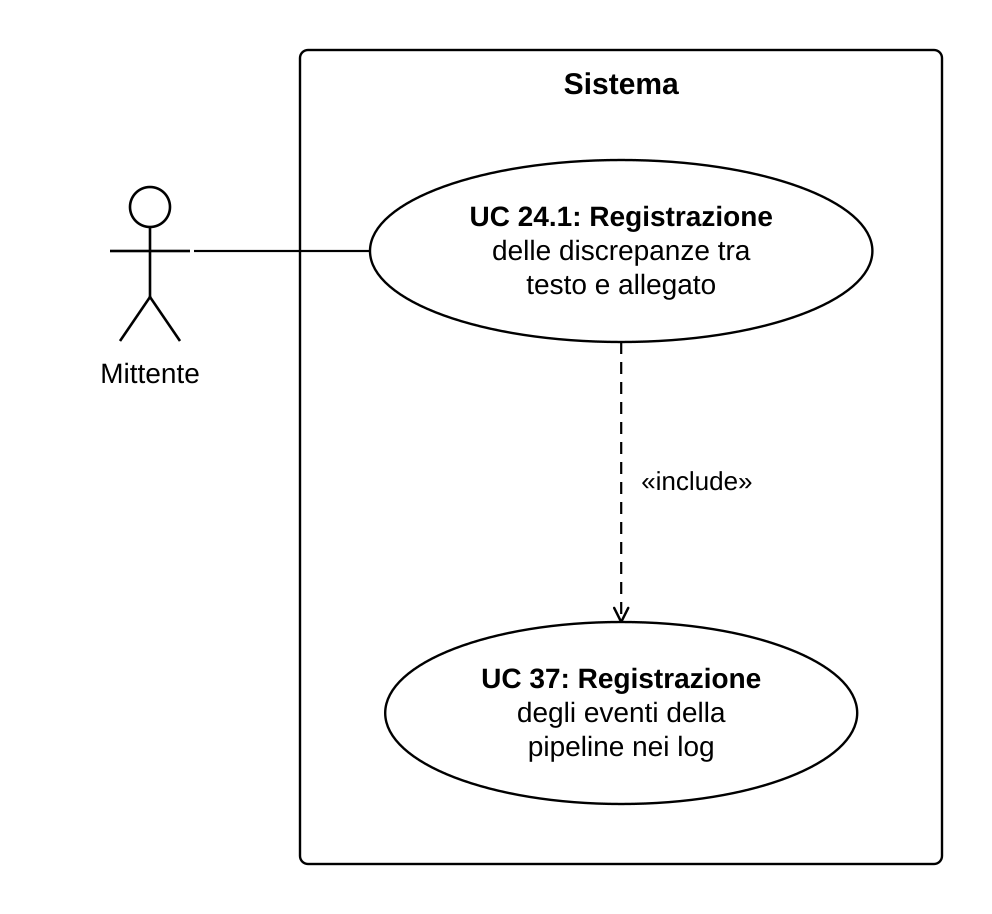
\includegraphics[width=\linewidth,height=0.32\textheight,keepaspectratio]{img/UC24_1.png}
\caption{UC 24.1 -- Registrazione delle discrepanze tra testo e allegato}
\end{center}
\begin{itemize}
    \item \textbf{Attore principale}: Mittente
    \item \textbf{Precondizioni}: Il sistema sta applicando la priorità al testo.
    \item \textbf{Scenario principale}:
    \begin{enumerate}
        \item Il sistema confronta i dati del testo con quelli dell'allegato.
        \item Il sistema registra nei log le discrepanze riscontrate (\hyperref[uc:37]{UC 37}).
    \end{enumerate}
    \item \textbf{Postcondizioni}: Le discrepanze sono registrate nei log.
    \item \textbf{Trigger}: Presenza di dati discordanti tra testo e allegato.
    \item \textbf{Inclusioni}:
    \begin{itemize}
        \item \hyperref[uc:37]{UC 37}: Registrazione degli eventi della pipeline nei log
    \end{itemize}
    \item \textbf{Incluso da}: \hyperref[uc:24]{UC 24}.
\end{itemize}

\subsubsection{UC 25: Scomposizione di un messaggio in richieste indipendenti}\label{uc:25}
\begin{center}
\captionsetup{type=figure}
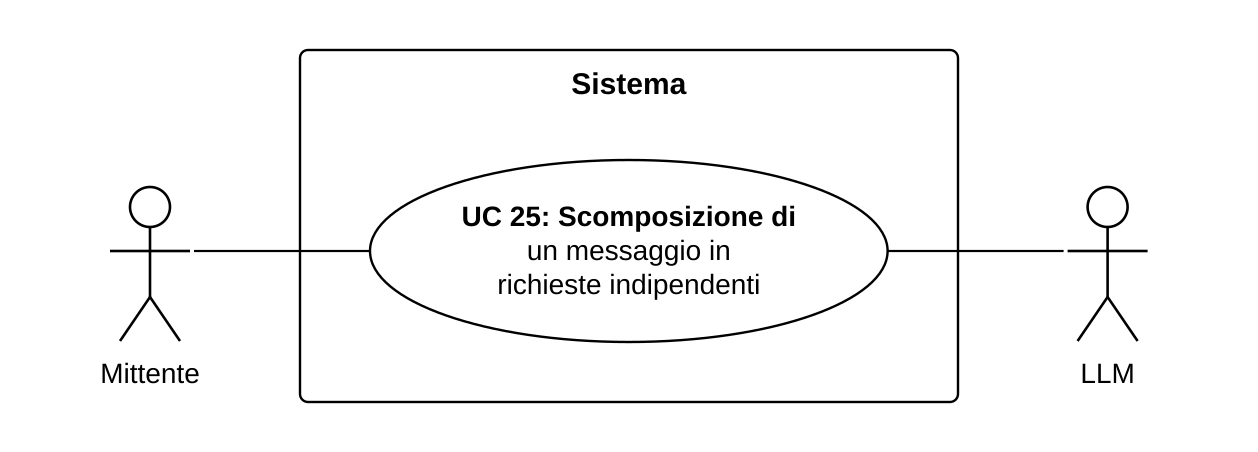
\includegraphics[width=\linewidth,height=0.32\textheight,keepaspectratio]{img/UC25.png}
\caption{UC 25 -- Scomposizione di un messaggio in richieste indipendenti}
\end{center}
\begin{itemize}
    \item \textbf{Attore principale}: Mittente
    \item \textbf{Attori secondari}: LLM
    \item \textbf{Precondizioni}: Il messaggio contiene più richieste distinte e il servizio LLM è raggiungibile.
    \item \textbf{Scenario principale}:
    \begin{enumerate}
        \item Il sistema individua le richieste distinte tramite l'LLM.
        \item Il sistema crea una richiesta indipendente per ciascuna.
        \item Il sistema traccia il messaggio di origine.
    \end{enumerate}
    \item \textbf{Postcondizioni}: Le richieste sono indipendenti e collegate al messaggio di origine.
    \item \textbf{Trigger}: Messaggio con più richieste distinte.
\end{itemize}

% ------------------------------------------------------------
% MACROAREA 5 --- AZIONI, INTEGRAZIONE E GESTIONE DELLE ANOMALIE
% ------------------------------------------------------------
\subsection{Macroarea 5 --- Azioni, integrazione e gestione delle anomalie}

\subsubsection{UC 26: Avvio automatico di azioni secondo le regole configurate}\label{uc:26}
\begin{center}
\captionsetup{type=figure}
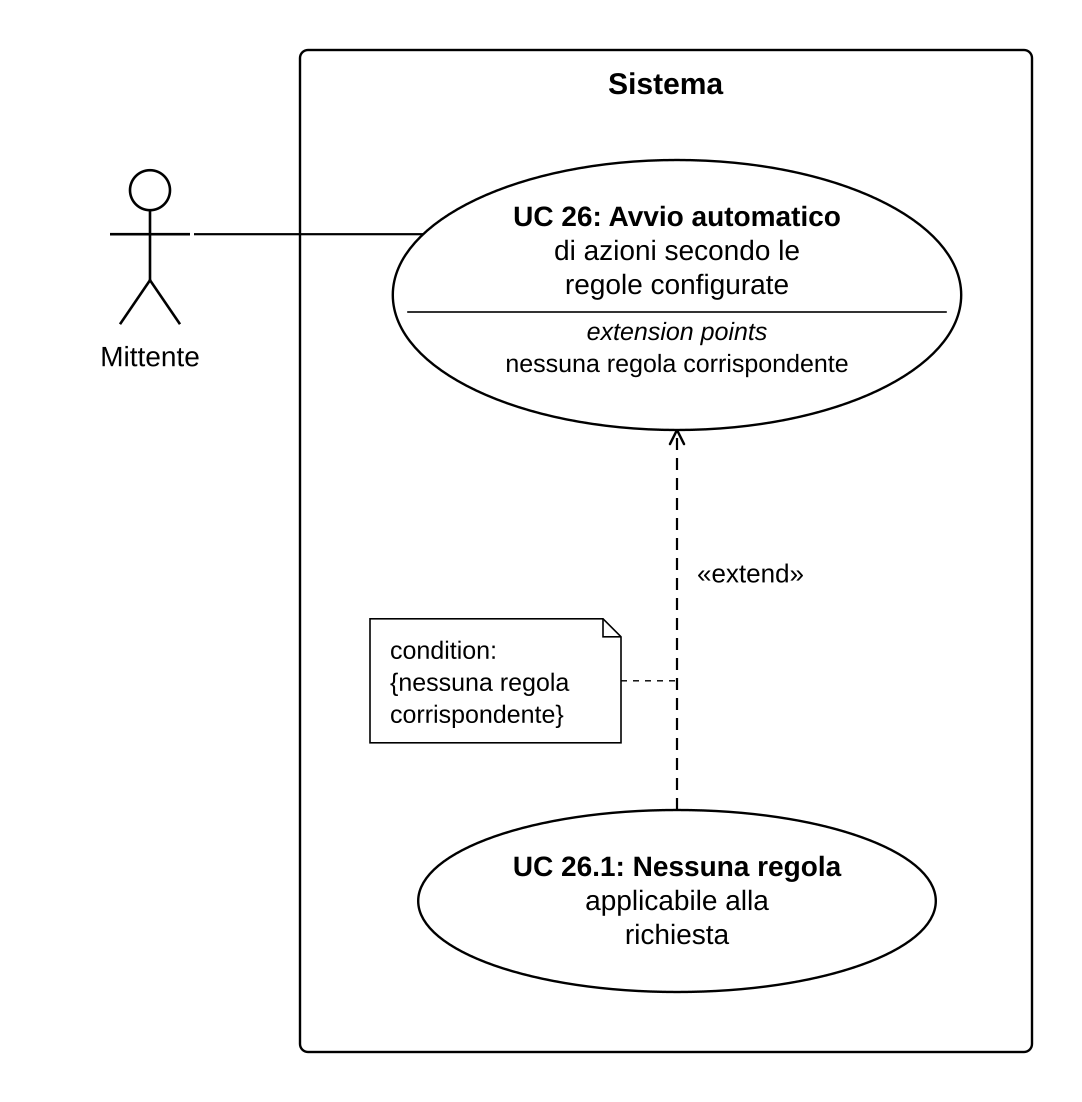
\includegraphics[width=\linewidth,height=0.32\textheight,keepaspectratio]{img/UC26.png}
\caption{UC 26 -- Avvio automatico di azioni secondo le regole configurate}
\end{center}
\begin{itemize}
    \item \textbf{Attore principale}: Mittente
    \item \textbf{Precondizioni}: La richiesta è stata strutturata e le regole di azione e notifica sono configurate.
    \item \textbf{Scenario principale}:
    \begin{enumerate}
        \item Il sistema individua la regola applicabile all'entità rilevata.
        \item Il sistema avvia l'azione associata alla regola.
    \end{enumerate}
    \item \textbf{Postcondizioni}: L'azione prevista dalla regola è avviata.
    \item \textbf{Trigger}: Completamento della strutturazione della richiesta.
    \item \textbf{Estensioni}:
    \begin{itemize}
        \item \hyperref[uc:26.1]{UC 26.1}: Nessuna regola applicabile alla richiesta $\rightarrow$ Condizione: Nessuna regola corrispondente.
    \end{itemize}
\end{itemize}

\subsubsection{UC 26.1: Nessuna regola applicabile alla richiesta}\label{uc:26.1}
\begin{center}
\captionsetup{type=figure}
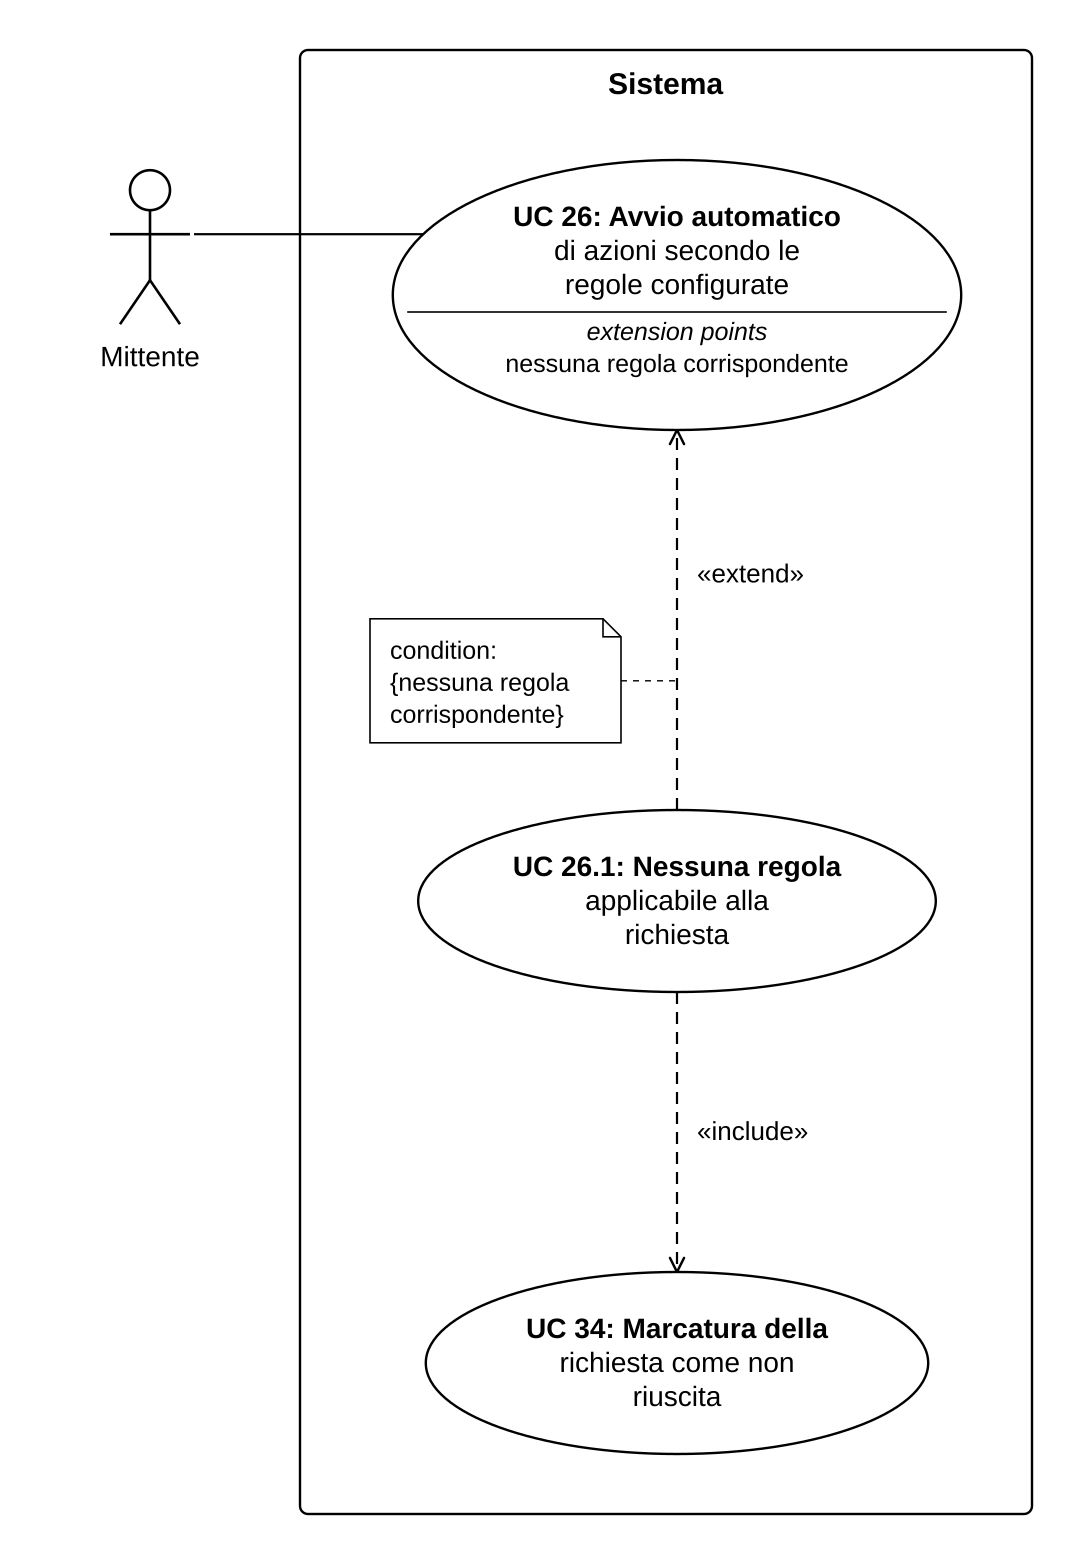
\includegraphics[width=\linewidth,height=0.32\textheight,keepaspectratio]{img/UC26_1.png}
\caption{UC 26.1 -- Nessuna regola applicabile alla richiesta}
\end{center}
\begin{itemize}
    \item \textbf{Attore principale}: Mittente
    \item \textbf{Precondizioni}: La ricerca della regola applicabile è in corso.
    \item \textbf{Scenario principale}:
    \begin{enumerate}
        \item Il sistema rileva che non esiste alcuna regola applicabile.
        \item Il sistema marca la richiesta come non riuscita (\hyperref[uc:34]{UC 34}).
        \item Il sistema registra l'evento nei log (\hyperref[uc:37]{UC 37}).
    \end{enumerate}
    \item \textbf{Postcondizioni}: La richiesta è marcata come non riuscita e l'evento è registrato nei log.
    \item \textbf{Trigger}: Nessuna regola corrispondente alla richiesta.
    \item \textbf{Estende}: \hyperref[uc:26]{UC 26}.
    \item \textbf{Inclusioni}:
    \begin{itemize}
        \item \hyperref[uc:34]{UC 34}: Marcatura della richiesta come non riuscita
    \end{itemize}
\end{itemize}

\subsubsection{UC 27: Inoltro dei dati strutturati agli applicativi tramite API REST}\label{uc:27}
\begin{center}
\captionsetup{type=figure}
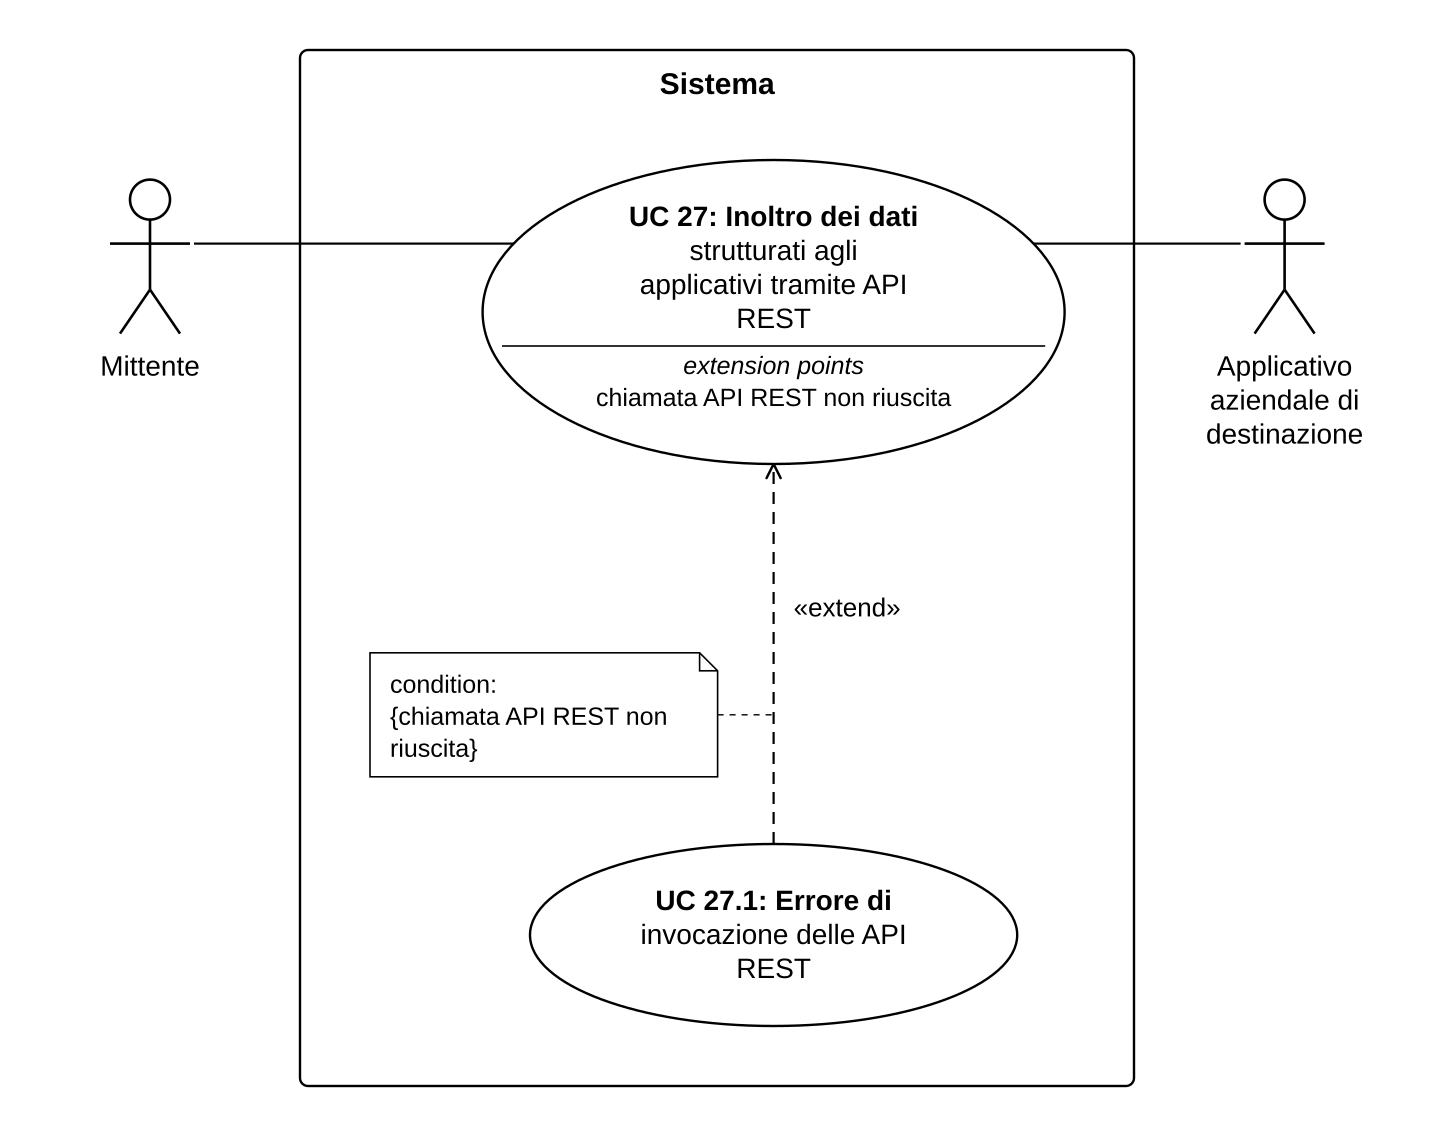
\includegraphics[width=\linewidth,height=0.32\textheight,keepaspectratio]{img/UC27.png}
\caption{UC 27 -- Inoltro dei dati strutturati agli applicativi tramite API REST}
\end{center}
\begin{itemize}
    \item \textbf{Attore principale}: Mittente
    \item \textbf{Attori secondari}: Applicativo aziendale di destinazione
    \item \textbf{Precondizioni}: Esiste un payload valido e l'applicativo di destinazione è configurato.
    \item \textbf{Scenario principale}:
    \begin{enumerate}
        \item Il sistema compone la chiamata API REST con i dati strutturati.
        \item Il sistema invoca l'applicativo di destinazione.
        \item L'applicativo conferma la ricezione dei dati.
        \item Il sistema aggiorna lo stato della richiesta.
    \end{enumerate}
    \item \textbf{Postcondizioni}: I dati sono inoltrati all'applicativo di destinazione.
    \item \textbf{Trigger}: Avvio di un'azione di inoltro.
    \item \textbf{Estensioni}:
    \begin{itemize}
        \item \hyperref[uc:27.1]{UC 27.1}: Errore di invocazione delle API REST $\rightarrow$ Condizione: Chiamata API REST non riuscita.
    \end{itemize}
    \item \textbf{Specializzazioni}: \hyperref[uc:28]{UC 28}, \hyperref[uc:29]{UC 29}, \hyperref[uc:30]{UC 30}, \hyperref[uc:31]{UC 31}, \hyperref[uc:32]{UC 32}.
\end{itemize}

\subsubsection{UC 27.1: Errore di invocazione delle API REST}\label{uc:27.1}
\begin{center}
\captionsetup{type=figure}
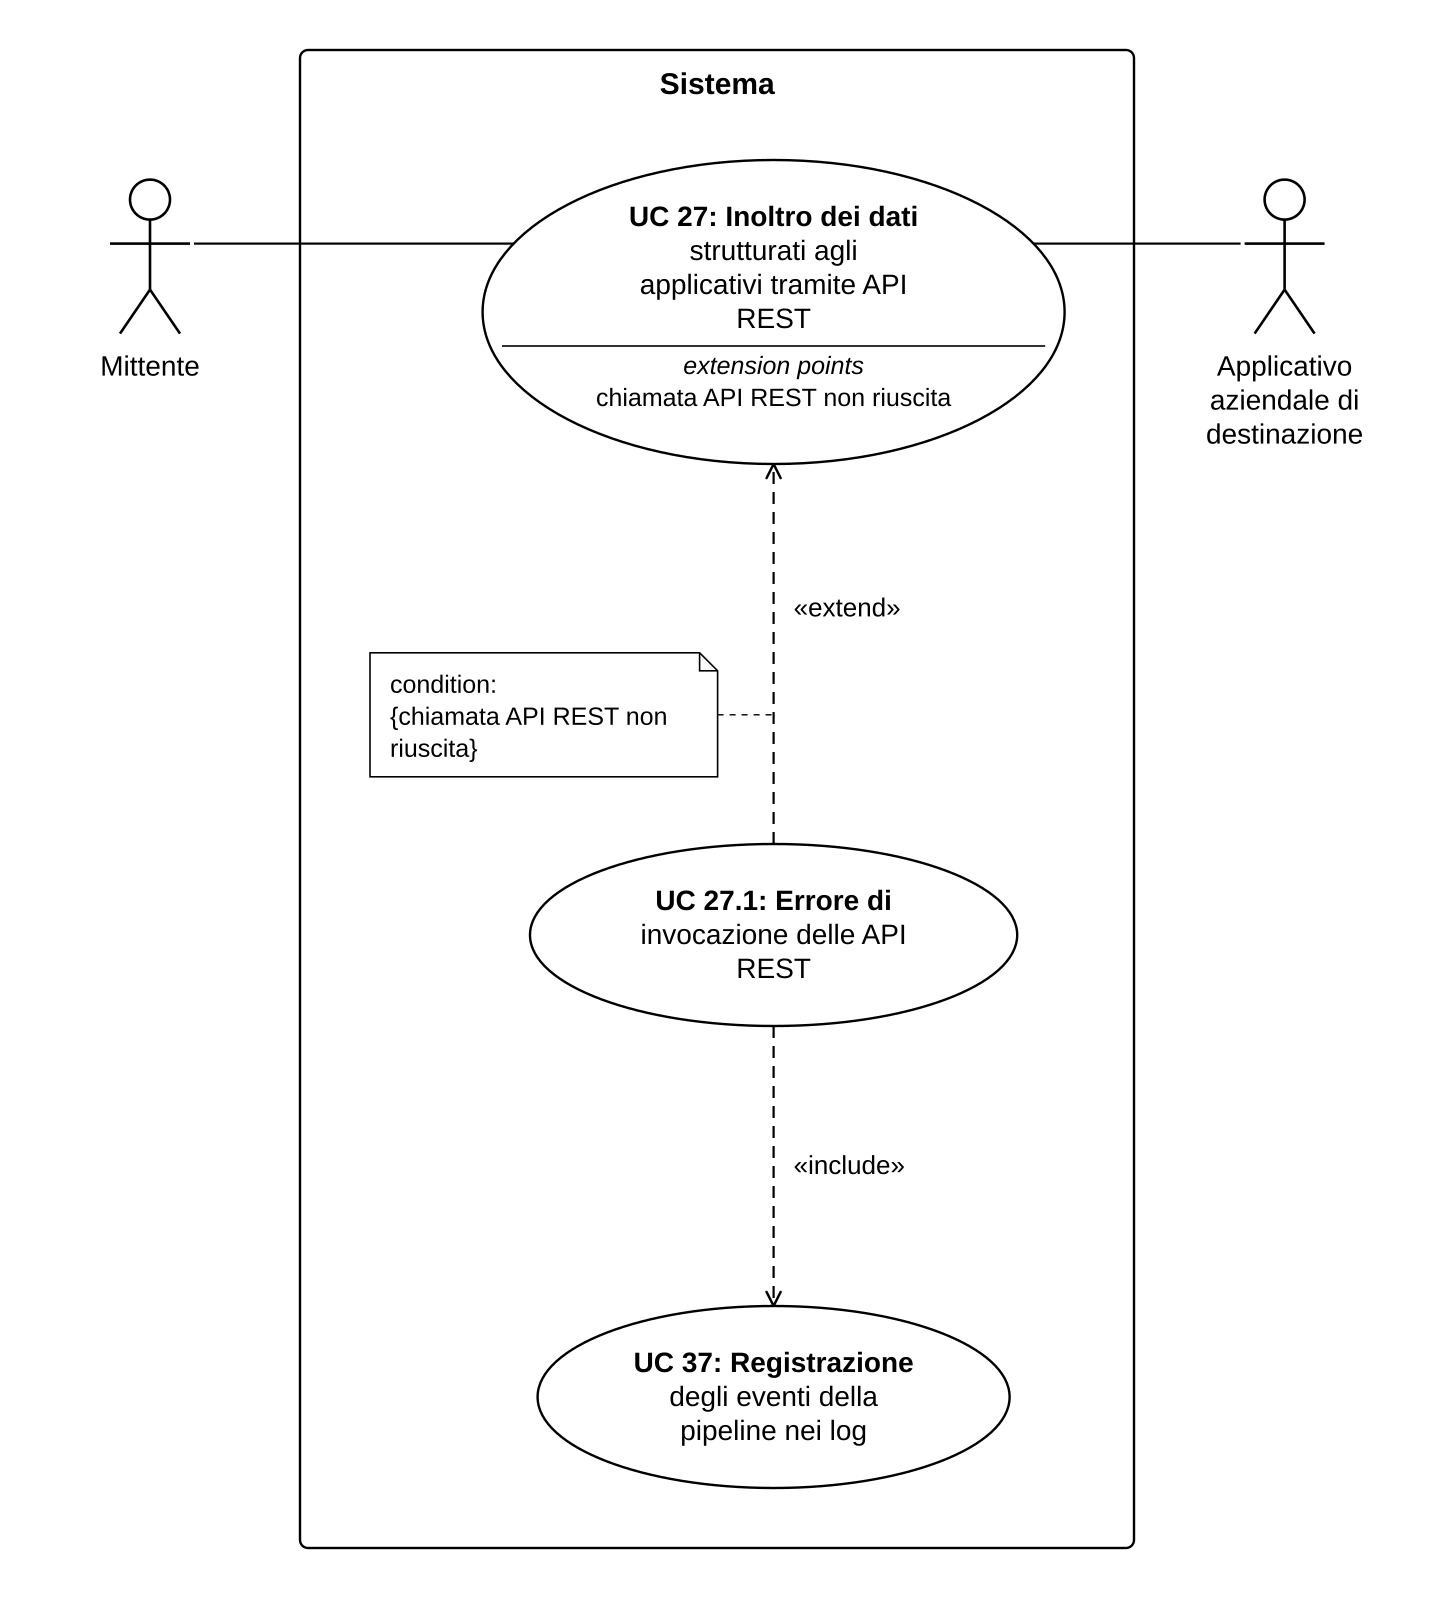
\includegraphics[width=\linewidth,height=0.32\textheight,keepaspectratio]{img/UC27_1.png}
\caption{UC 27.1 -- Errore di invocazione delle API REST}
\end{center}
\begin{itemize}
    \item \textbf{Attore principale}: Mittente
    \item \textbf{Precondizioni}: L'invocazione dell'API REST è in corso.
    \item \textbf{Scenario principale}:
    \begin{enumerate}
        \item Il sistema rileva un errore nella chiamata.
        \item Il sistema registra l'errore nei log (\hyperref[uc:37]{UC 37}).
        \item Il sistema imposta la richiesta in stato di inoltro fallito.
    \end{enumerate}
    \item \textbf{Postcondizioni}: La richiesta è in stato di inoltro fallito e l'errore è registrato nei log.
    \item \textbf{Trigger}: Chiamata API REST non riuscita.
    \item \textbf{Estende}: \hyperref[uc:27]{UC 27}.
    \item \textbf{Inclusioni}:
    \begin{itemize}
        \item \hyperref[uc:37]{UC 37}: Registrazione degli eventi della pipeline nei log
    \end{itemize}
\end{itemize}

\subsubsection{UC 28: Creazione automatica dell'ordine d'acquisto sul portale B2B}\label{uc:28}
\begin{center}
\captionsetup{type=figure}
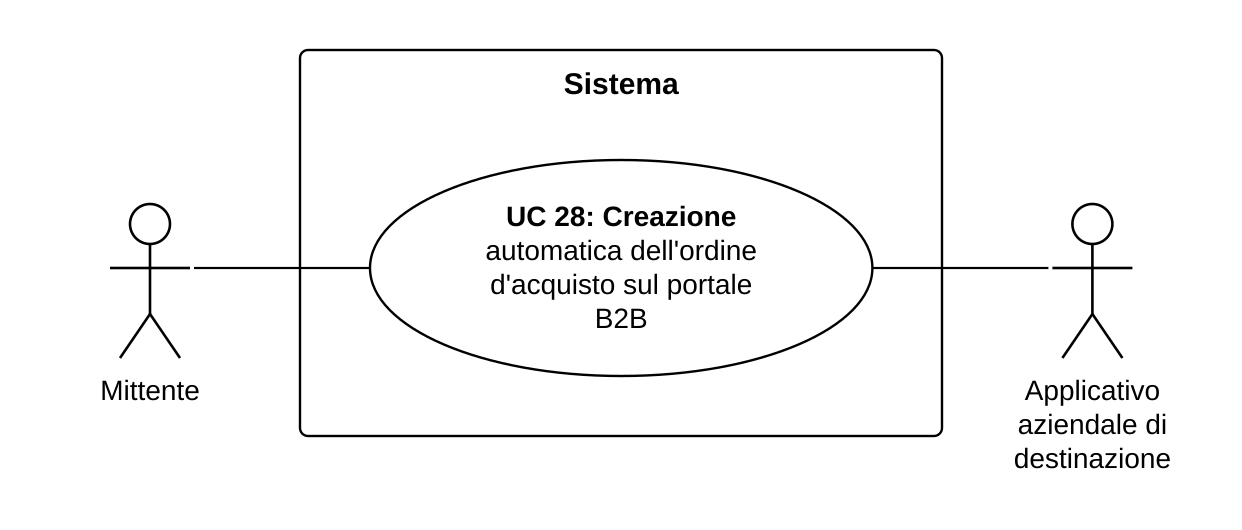
\includegraphics[width=\linewidth,height=0.32\textheight,keepaspectratio]{img/UC28.png}
\caption{UC 28 -- Creazione automatica dell'ordine d'acquisto sul portale B2B}
\end{center}
\begin{itemize}
    \item \textbf{Attore principale}: Mittente
    \item \textbf{Attori secondari}: Applicativo aziendale di destinazione
    \item \textbf{Precondizioni}: La richiesta è un ordine validato e il portale B2B è configurato.
    \item \textbf{Scenario principale}:
    \begin{enumerate}
        \item Il sistema inoltra il payload al portale B2B (\hyperref[uc:27]{UC 27}).
        \item Il portale B2B crea l'ordine d'acquisto.
        \item Il sistema aggiorna lo stato della richiesta.
    \end{enumerate}
    \item \textbf{Postcondizioni}: L'ordine d'acquisto è creato sul portale B2B senza intervento umano.
    \item \textbf{Trigger}: Disponibilità di una richiesta d'ordine validata.
    \item \textbf{Specializza}: \hyperref[uc:27]{UC 27}.
\end{itemize}

\subsubsection{UC 29: Apertura automatica di un ticket di assistenza}\label{uc:29}
\begin{center}
\captionsetup{type=figure}
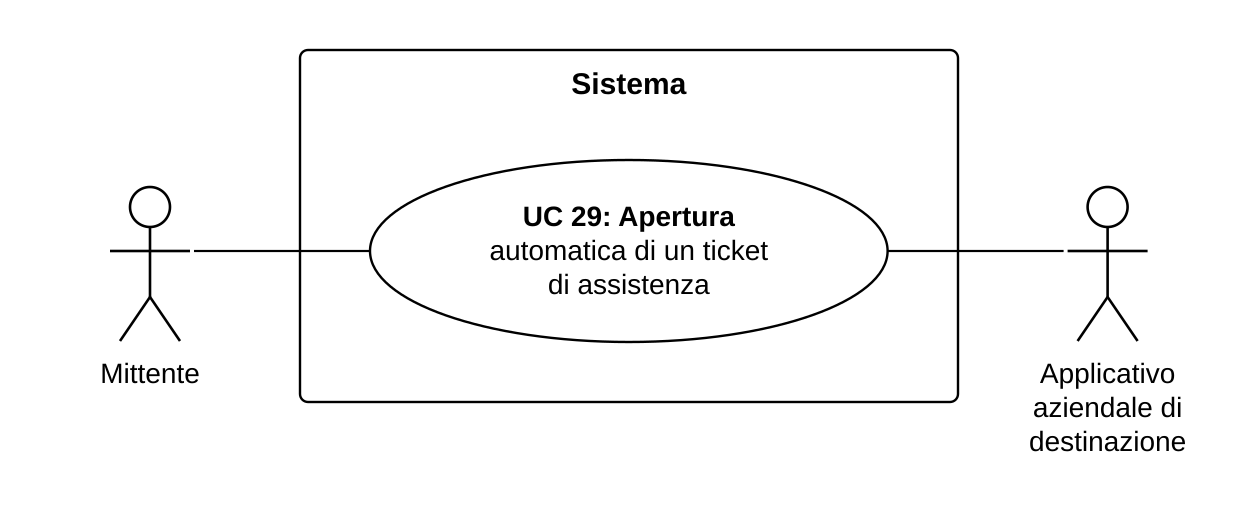
\includegraphics[width=\linewidth,height=0.32\textheight,keepaspectratio]{img/UC29.png}
\caption{UC 29 -- Apertura automatica di un ticket di assistenza}
\end{center}
\begin{itemize}
    \item \textbf{Attore principale}: Mittente
    \item \textbf{Attori secondari}: Applicativo aziendale di destinazione
    \item \textbf{Precondizioni}: La richiesta è di assistenza e l'applicativo di ticketing è configurato.
    \item \textbf{Scenario principale}:
    \begin{enumerate}
        \item Il sistema inoltra il payload all'applicativo di ticketing (\hyperref[uc:27]{UC 27}).
        \item L'applicativo apre il ticket di assistenza.
        \item Il sistema aggiorna lo stato della richiesta.
    \end{enumerate}
    \item \textbf{Postcondizioni}: Il ticket di assistenza è aperto.
    \item \textbf{Trigger}: Disponibilità di una richiesta di assistenza.
    \item \textbf{Specializza}: \hyperref[uc:27]{UC 27}.
\end{itemize}

\subsubsection{UC 30: Registrazione automatica di un appuntamento}\label{uc:30}
\begin{center}
\captionsetup{type=figure}
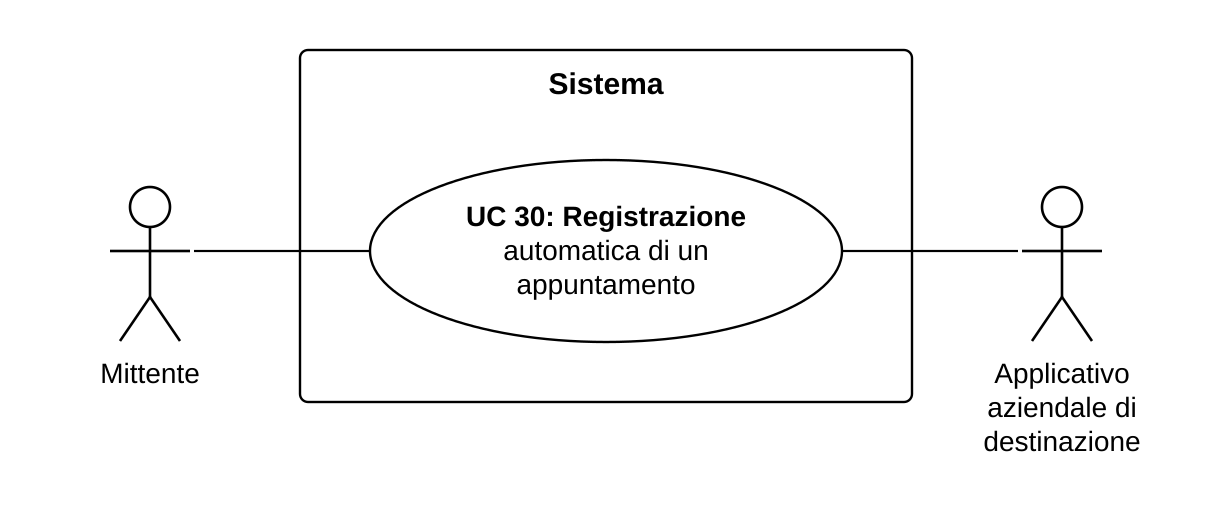
\includegraphics[width=\linewidth,height=0.32\textheight,keepaspectratio]{img/UC30.png}
\caption{UC 30 -- Registrazione automatica di un appuntamento}
\end{center}
\begin{itemize}
    \item \textbf{Attore principale}: Mittente
    \item \textbf{Attori secondari}: Applicativo aziendale di destinazione
    \item \textbf{Precondizioni}: La richiesta è di prenotazione e l'applicativo di destinazione è configurato.
    \item \textbf{Scenario principale}:
    \begin{enumerate}
        \item Il sistema inoltra il payload all'applicativo (\hyperref[uc:27]{UC 27}).
        \item L'applicativo registra l'appuntamento.
        \item Il sistema aggiorna lo stato della richiesta.
    \end{enumerate}
    \item \textbf{Postcondizioni}: L'appuntamento è registrato.
    \item \textbf{Trigger}: Disponibilità di una richiesta di prenotazione.
    \item \textbf{Specializza}: \hyperref[uc:27]{UC 27}.
\end{itemize}

\subsubsection{UC 31: Registrazione automatica di un'opportunità commerciale nel CRM}\label{uc:31}
\begin{center}
\captionsetup{type=figure}
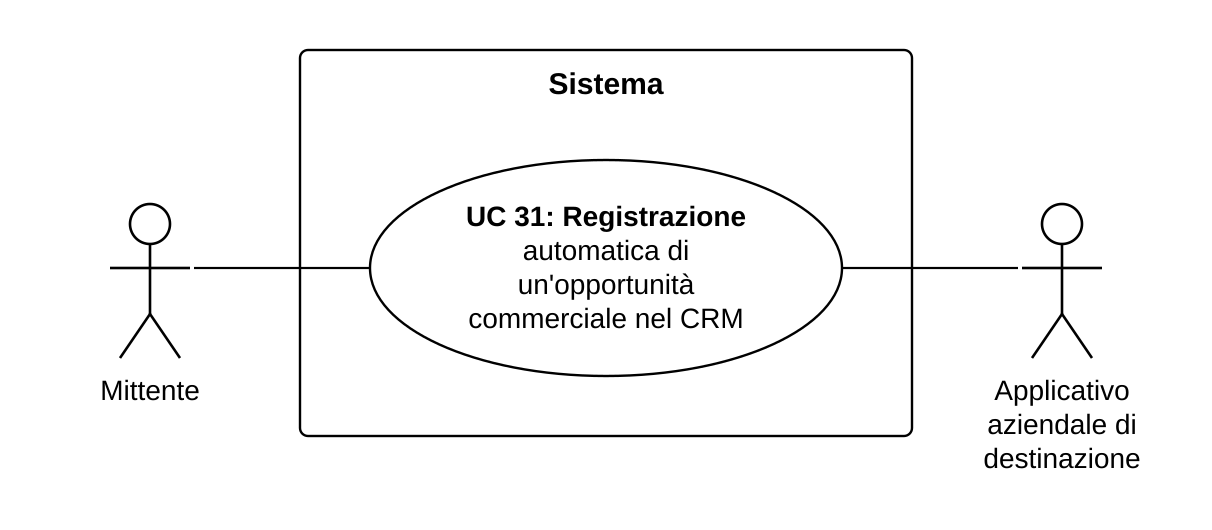
\includegraphics[width=\linewidth,height=0.32\textheight,keepaspectratio]{img/UC31.png}
\caption{UC 31 -- Registrazione automatica di un'opportunità commerciale nel CRM}
\end{center}
\begin{itemize}
    \item \textbf{Attore principale}: Mittente
    \item \textbf{Attori secondari}: Applicativo aziendale di destinazione
    \item \textbf{Precondizioni}: La richiesta è una segnalazione commerciale e il CRM è configurato.
    \item \textbf{Scenario principale}:
    \begin{enumerate}
        \item Il sistema inoltra il payload al CRM (\hyperref[uc:27]{UC 27}).
        \item Il CRM registra l'opportunità commerciale.
        \item Il sistema aggiorna lo stato della richiesta.
    \end{enumerate}
    \item \textbf{Postcondizioni}: L'opportunità commerciale è registrata nel CRM.
    \item \textbf{Trigger}: Disponibilità di una segnalazione commerciale.
    \item \textbf{Specializza}: \hyperref[uc:27]{UC 27}.
\end{itemize}

\subsubsection{UC 32: Inoltro all'ERP di una richiesta di documento contabile}\label{uc:32}
\begin{center}
\captionsetup{type=figure}
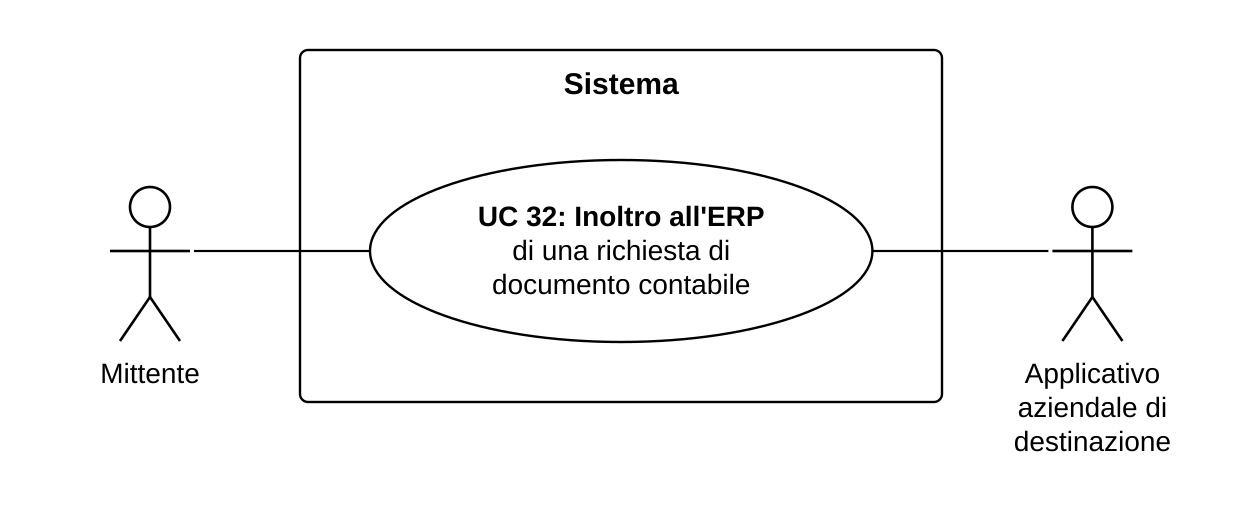
\includegraphics[width=\linewidth,height=0.32\textheight,keepaspectratio]{img/UC32.png}
\caption{UC 32 -- Inoltro all'ERP di una richiesta di documento contabile}
\end{center}
\begin{itemize}
    \item \textbf{Attore principale}: Mittente
    \item \textbf{Attori secondari}: Applicativo aziendale di destinazione
    \item \textbf{Precondizioni}: La richiesta riguarda un documento contabile e l'ERP è configurato.
    \item \textbf{Scenario principale}:
    \begin{enumerate}
        \item Il sistema inoltra il payload all'ERP (\hyperref[uc:27]{UC 27}).
        \item L'ERP prende in carico la richiesta.
        \item Il sistema aggiorna lo stato della richiesta.
    \end{enumerate}
    \item \textbf{Postcondizioni}: La richiesta è inoltrata all'ERP.
    \item \textbf{Trigger}: Disponibilità di una richiesta di documento contabile o fatturazione.
    \item \textbf{Specializza}: \hyperref[uc:27]{UC 27}.
\end{itemize}

\subsubsection{UC 33: Invio automatico di e-mail di notifica}\label{uc:33}
\begin{center}
\captionsetup{type=figure}
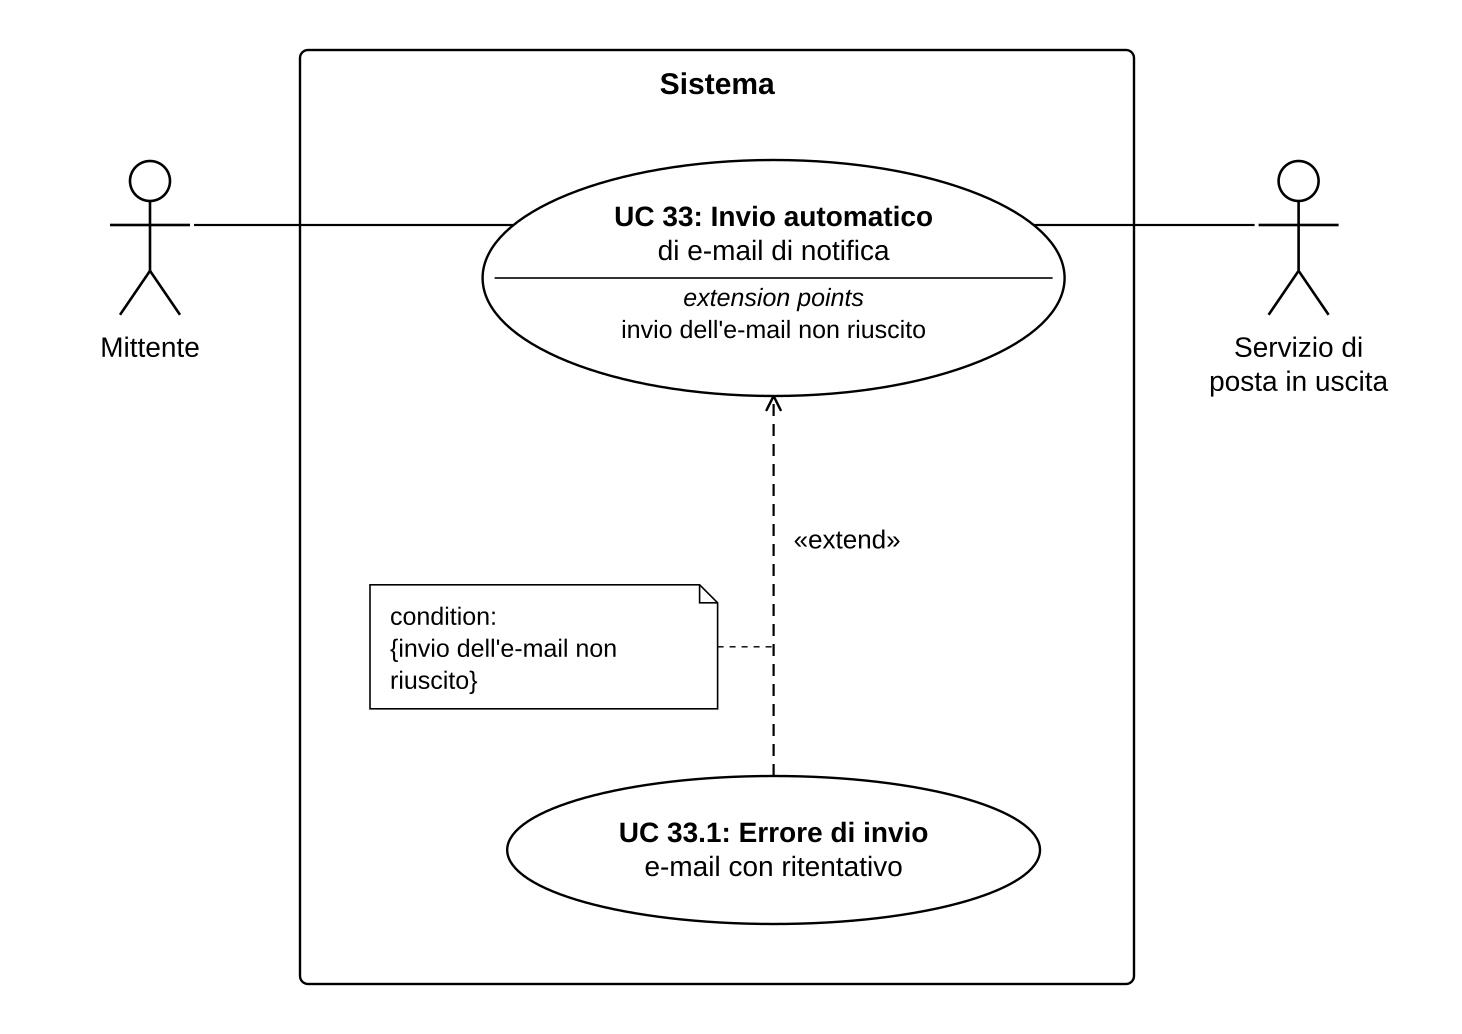
\includegraphics[width=\linewidth,height=0.32\textheight,keepaspectratio]{img/UC33.png}
\caption{UC 33 -- Invio automatico di e-mail di notifica}
\end{center}
\begin{itemize}
    \item \textbf{Attore principale}: Mittente
    \item \textbf{Attori secondari}: Servizio di posta in uscita
    \item \textbf{Precondizioni}: Una regola prevede l'invio di una notifica e il servizio di posta in uscita è configurato.
    \item \textbf{Scenario principale}:
    \begin{enumerate}
        \item Il sistema compone l'e-mail di notifica secondo la regola.
        \item Il sistema la invia tramite il servizio di posta in uscita.
        \item Il sistema registra l'esito dell'invio.
    \end{enumerate}
    \item \textbf{Postcondizioni}: L'e-mail di notifica è inviata.
    \item \textbf{Trigger}: Applicazione di una regola di notifica.
    \item \textbf{Estensioni}:
    \begin{itemize}
        \item \hyperref[uc:33.1]{UC 33.1}: Errore di invio e-mail con ritentativo $\rightarrow$ Condizione: Invio dell'e-mail non riuscito.
    \end{itemize}
\end{itemize}

\subsubsection{UC 33.1: Errore di invio e-mail con ritentativo}\label{uc:33.1}
\begin{center}
\captionsetup{type=figure}
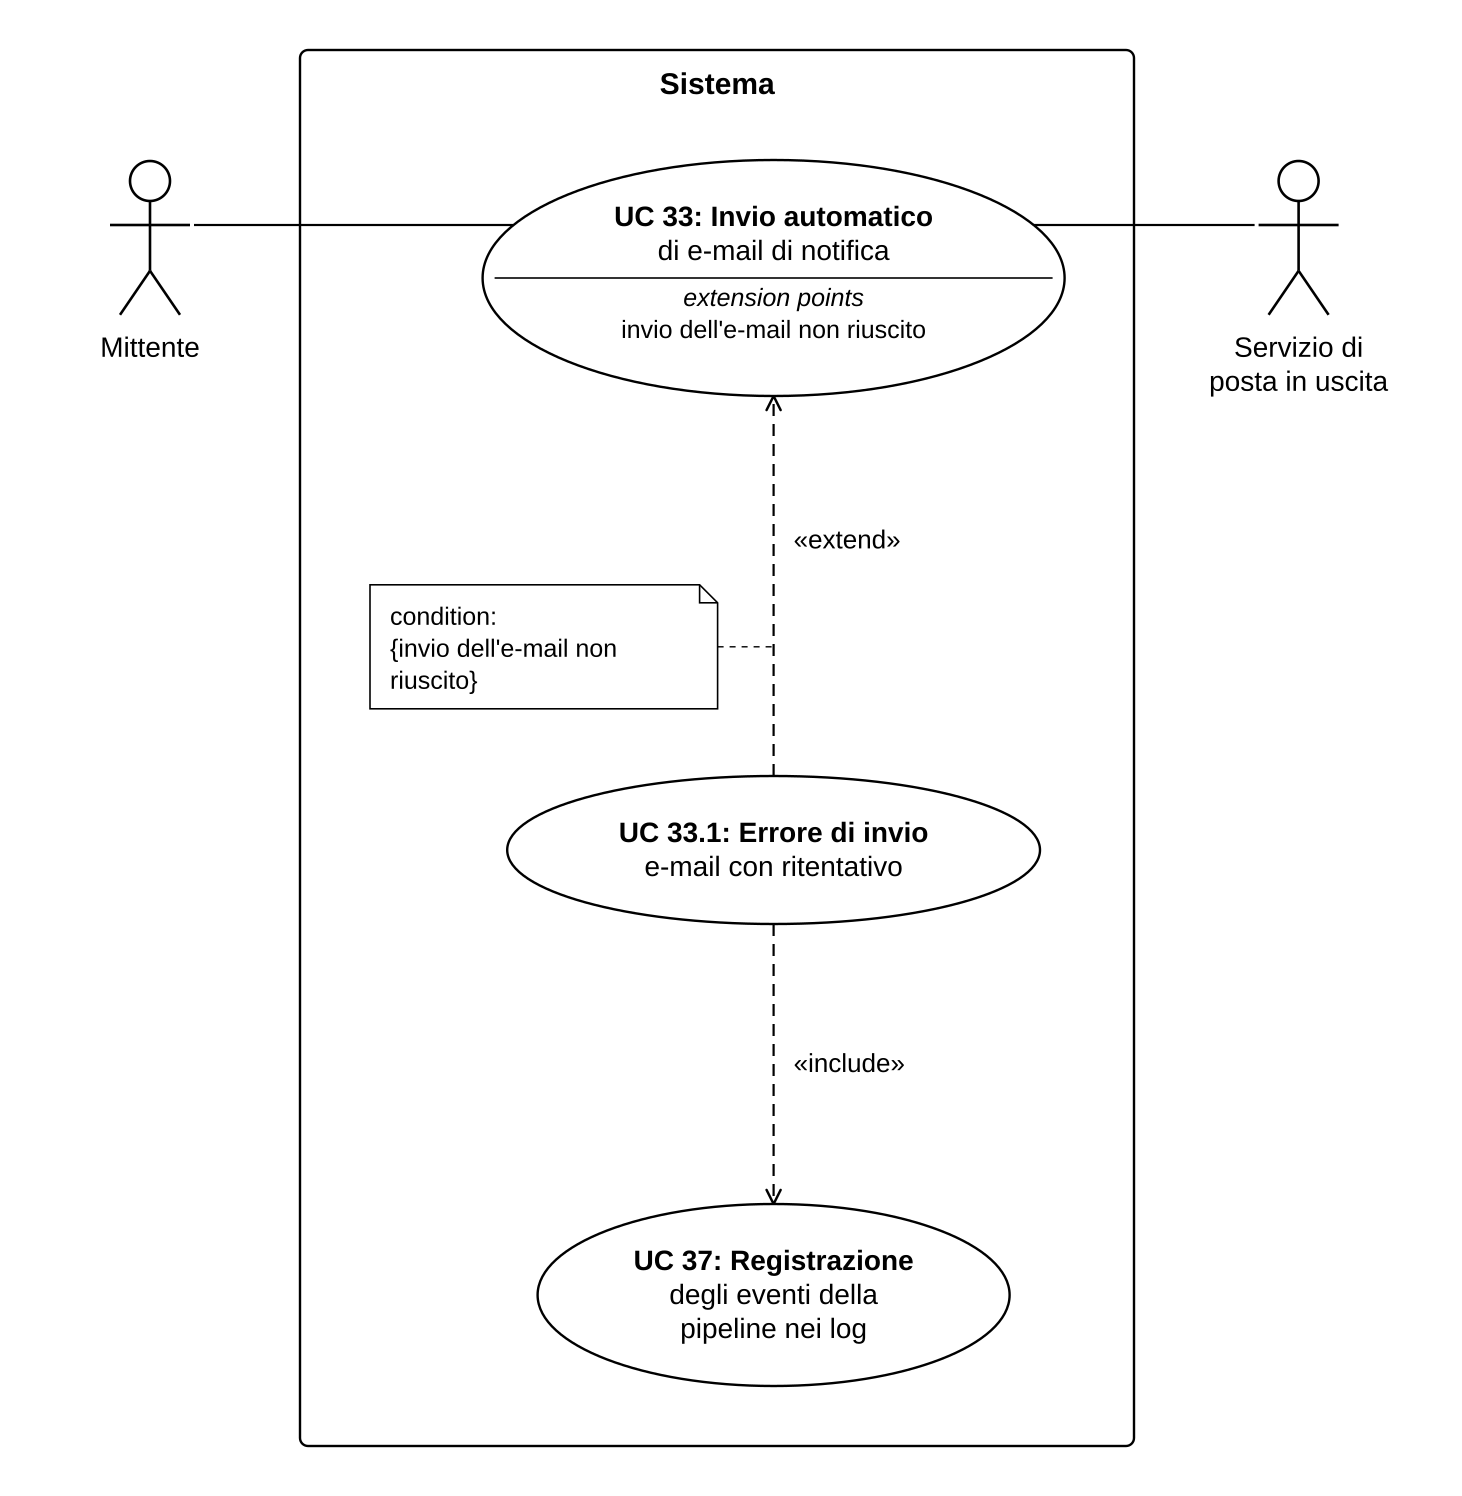
\includegraphics[width=\linewidth,height=0.32\textheight,keepaspectratio]{img/UC33_1.png}
\caption{UC 33.1 -- Errore di invio e-mail con ritentativo}
\end{center}
\begin{itemize}
    \item \textbf{Attore principale}: Mittente
    \item \textbf{Precondizioni}: L'invio dell'e-mail è in corso.
    \item \textbf{Scenario principale}:
    \begin{enumerate}
        \item Il sistema rileva un errore di invio.
        \item Il sistema registra l'errore nei log (\hyperref[uc:37]{UC 37}).
        \item Il sistema ritenta l'invio.
    \end{enumerate}
    \item \textbf{Postcondizioni}: L'errore è registrato e l'invio è ritentato.
    \item \textbf{Trigger}: Invio dell'e-mail non riuscito.
    \item \textbf{Estende}: \hyperref[uc:33]{UC 33}.
    \item \textbf{Inclusioni}:
    \begin{itemize}
        \item \hyperref[uc:37]{UC 37}: Registrazione degli eventi della pipeline nei log
    \end{itemize}
\end{itemize}

\subsubsection{UC 34: Marcatura della richiesta come non riuscita}\label{uc:34}
\begin{center}
\captionsetup{type=figure}
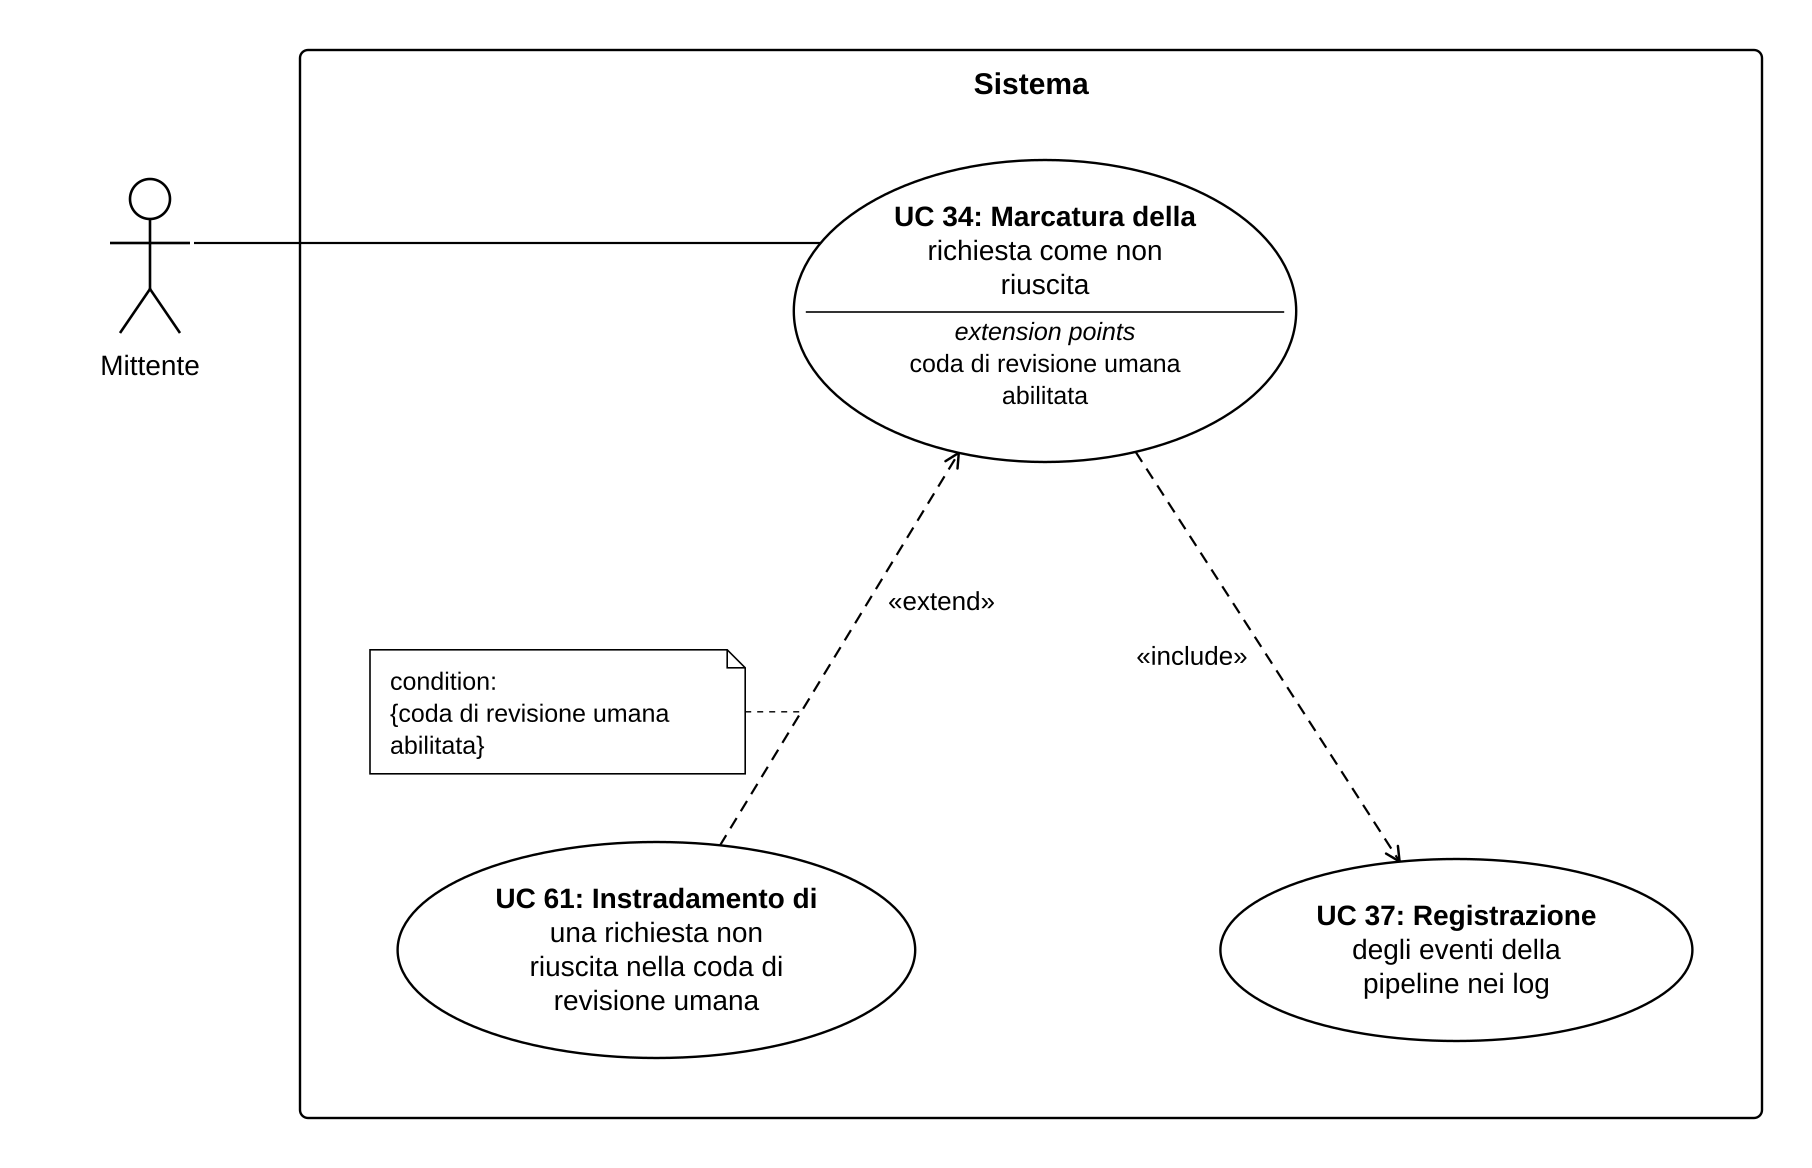
\includegraphics[width=\linewidth,height=0.32\textheight,keepaspectratio]{img/UC34.png}
\caption{UC 34 -- Marcatura della richiesta come non riuscita}
\end{center}
\begin{itemize}
    \item \textbf{Attore principale}: Mittente
    \item \textbf{Precondizioni}: Una richiesta non può essere elaborata con sufficiente affidabilità.
    \item \textbf{Scenario principale}:
    \begin{enumerate}
        \item Il sistema imposta lo stato della richiesta come non riuscita.
        \item Il sistema registra nei log il motivo e lo specifico elemento problematico (\hyperref[uc:37]{UC 37}).
    \end{enumerate}
    \item \textbf{Postcondizioni}: La richiesta è in stato non riuscita ed è consultabile tramite la dashboard.
    \item \textbf{Trigger}: Rilevamento di un'anomalia che impedisce l'elaborazione.
    \item \textbf{Inclusioni}:
    \begin{itemize}
        \item \hyperref[uc:37]{UC 37}: Registrazione degli eventi della pipeline nei log
    \end{itemize}
    \item \textbf{Estensioni}:
    \begin{itemize}
        \item \hyperref[uc:61]{UC 61}: Instradamento di una richiesta non riuscita nella coda di revisione umana $\rightarrow$ Condizione: Coda di revisione umana abilitata.
    \end{itemize}
\end{itemize}

\subsubsection{UC 35: Persistenza di testo estratto, payload e stato della richiesta}\label{uc:35}
\begin{center}
\captionsetup{type=figure}
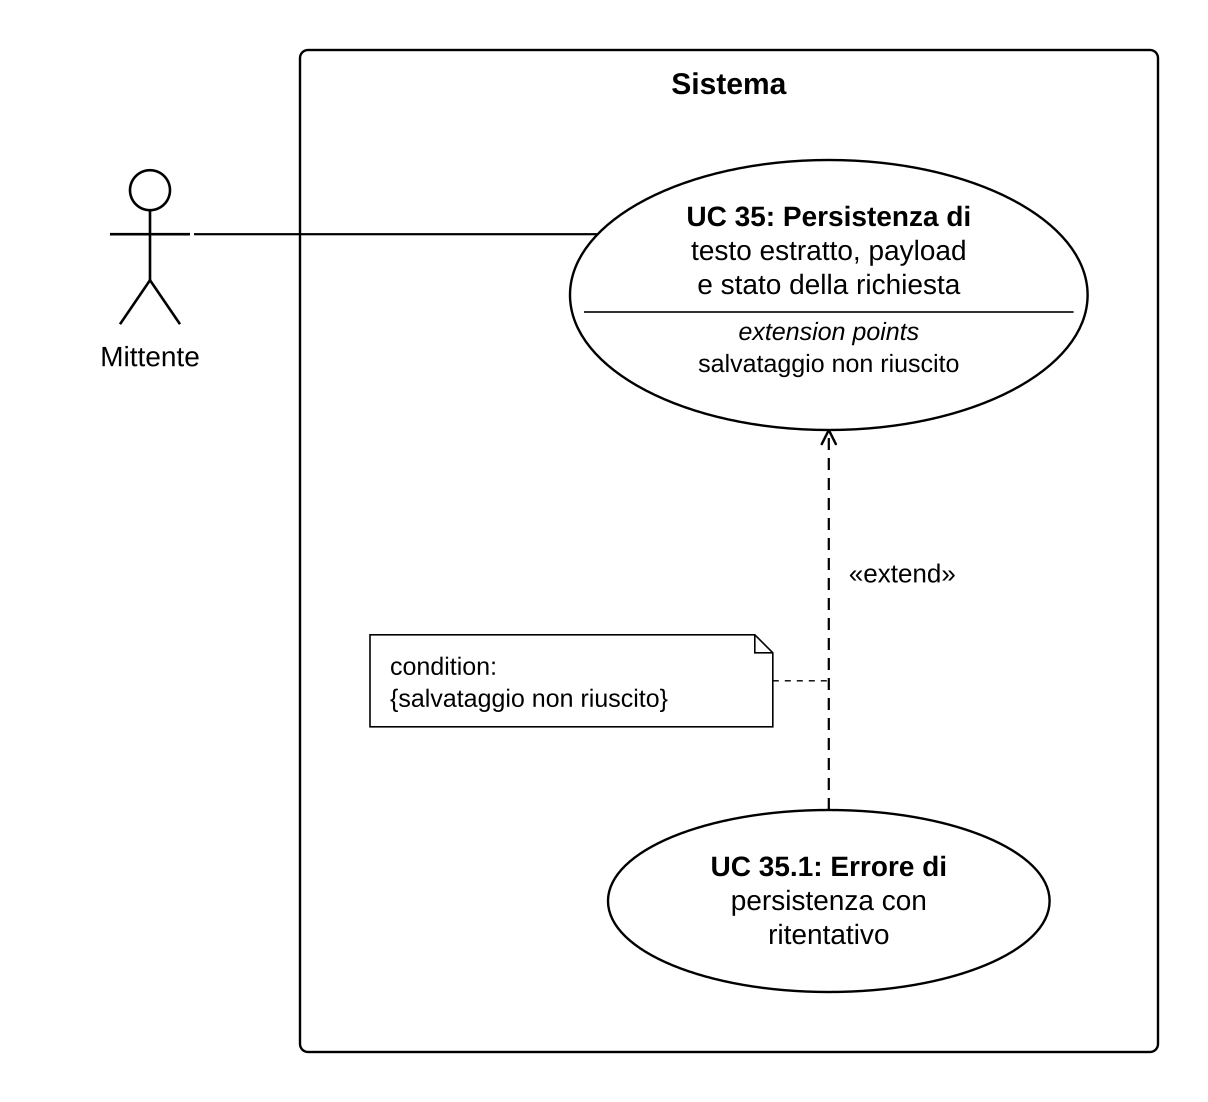
\includegraphics[width=\linewidth,height=0.32\textheight,keepaspectratio]{img/UC35.png}
\caption{UC 35 -- Persistenza di testo estratto, payload e stato della richiesta}
\end{center}
\begin{itemize}
    \item \textbf{Attore principale}: Mittente
    \item \textbf{Precondizioni}: È disponibile almeno un risultato di elaborazione della richiesta.
    \item \textbf{Scenario principale}:
    \begin{enumerate}
        \item Il sistema salva nel database relazionale testo estratto, payload JSON e stato di avanzamento.
        \item Il sistema conferma il salvataggio.
    \end{enumerate}
    \item \textbf{Postcondizioni}: I dati della richiesta sono persistiti.
    \item \textbf{Trigger}: Avanzamento della richiesta nella pipeline.
    \item \textbf{Estensioni}:
    \begin{itemize}
        \item \hyperref[uc:35.1]{UC 35.1}: Errore di persistenza con ritentativo $\rightarrow$ Condizione: Salvataggio non riuscito.
    \end{itemize}
\end{itemize}

\subsubsection{UC 35.1: Errore di persistenza con ritentativo}\label{uc:35.1}
\begin{center}
\captionsetup{type=figure}
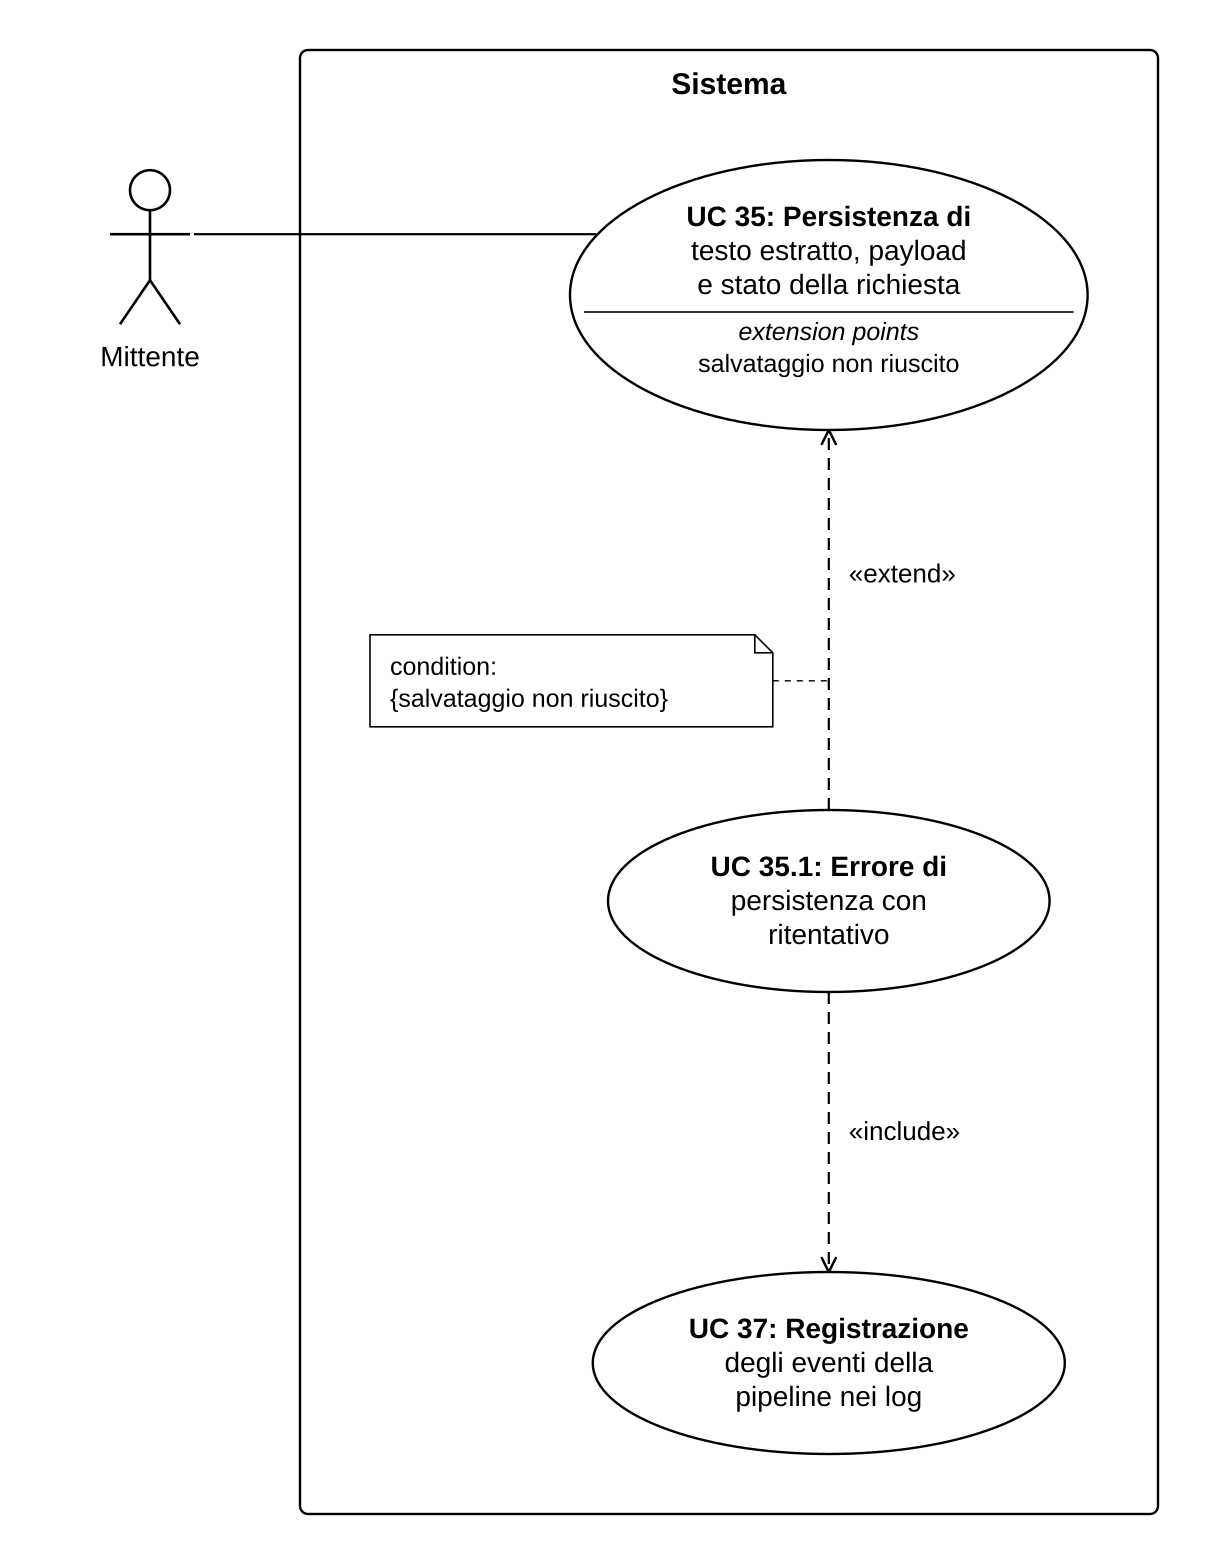
\includegraphics[width=\linewidth,height=0.32\textheight,keepaspectratio]{img/UC35_1.png}
\caption{UC 35.1 -- Errore di persistenza con ritentativo}
\end{center}
\begin{itemize}
    \item \textbf{Attore principale}: Mittente
    \item \textbf{Precondizioni}: Il salvataggio nel database è in corso.
    \item \textbf{Scenario principale}:
    \begin{enumerate}
        \item Il sistema rileva un errore di persistenza.
        \item Il sistema registra l'errore nei log (\hyperref[uc:37]{UC 37}).
        \item Il sistema ritenta il salvataggio senza perdere la richiesta.
    \end{enumerate}
    \item \textbf{Postcondizioni}: L'errore è registrato e il salvataggio è ritentato.
    \item \textbf{Trigger}: Salvataggio non riuscito.
    \item \textbf{Estende}: \hyperref[uc:35]{UC 35}.
    \item \textbf{Inclusioni}:
    \begin{itemize}
        \item \hyperref[uc:37]{UC 37}: Registrazione degli eventi della pipeline nei log
    \end{itemize}
\end{itemize}

\subsubsection{UC 36: Cifratura e salvataggio dei file originali allegati}\label{uc:36}
\begin{center}
\captionsetup{type=figure}
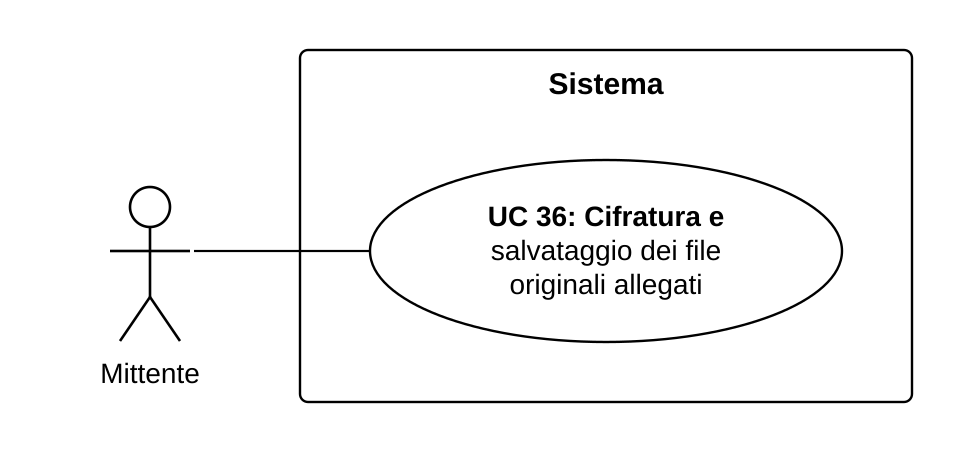
\includegraphics[width=\linewidth,height=0.32\textheight,keepaspectratio]{img/UC36.png}
\caption{UC 36 -- Cifratura e salvataggio dei file originali allegati}
\end{center}
\begin{itemize}
    \item \textbf{Attore principale}: Mittente
    \item \textbf{Precondizioni}: La richiesta ha file originali allegati (PDF, immagini, audio).
    \item \textbf{Scenario principale}:
    \begin{enumerate}
        \item Il sistema cifra i file originali.
        \item Il sistema salva i file cifrati su disco.
        \item Il sistema associa i file alla richiesta.
    \end{enumerate}
    \item \textbf{Postcondizioni}: I file originali sono salvati cifrati e utilizzabili per l'inoltro e il debugging.
    \item \textbf{Trigger}: Salvataggio dei file allegati di una richiesta.
\end{itemize}

\subsubsection{UC 37: Registrazione degli eventi della pipeline nei log}\label{uc:37}
\begin{center}
\captionsetup{type=figure}
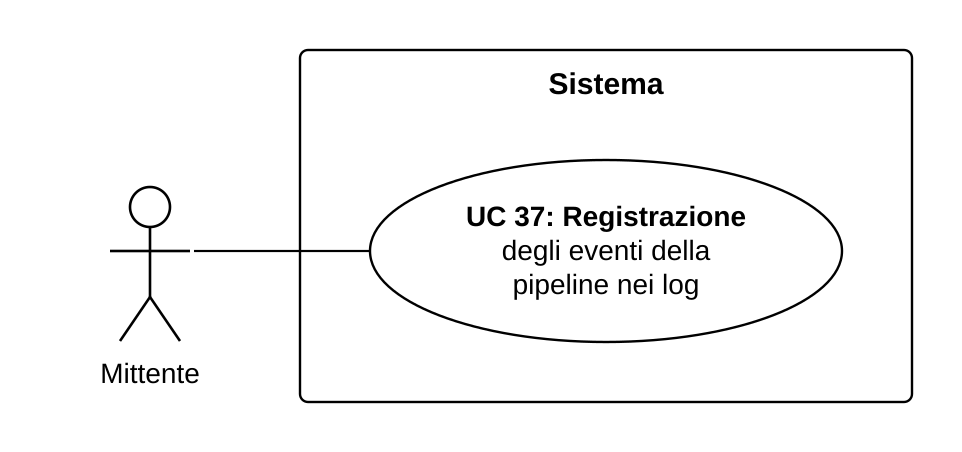
\includegraphics[width=\linewidth,height=0.32\textheight,keepaspectratio]{img/UC37.png}
\caption{UC 37 -- Registrazione degli eventi della pipeline nei log}
\end{center}
\begin{itemize}
    \item \textbf{Attore principale}: Mittente
    \item \textbf{Precondizioni}: Si è verificato un evento della pipeline.
    \item \textbf{Scenario principale}:
    \begin{enumerate}
        \item Il sistema registra nei log esito, anomalia o azione eseguita relativi alla richiesta.
    \end{enumerate}
    \item \textbf{Postcondizioni}: L'evento è registrato nei log.
    \item \textbf{Trigger}: Evento della pipeline da tracciare.
\end{itemize}


\subsection{Macroarea 6 --- Interfaccia amministrativa e profili di accesso}

\subsubsection{UC 38: Autenticazione utente}\label{uc:38}
\begin{center}
\captionsetup{type=figure}
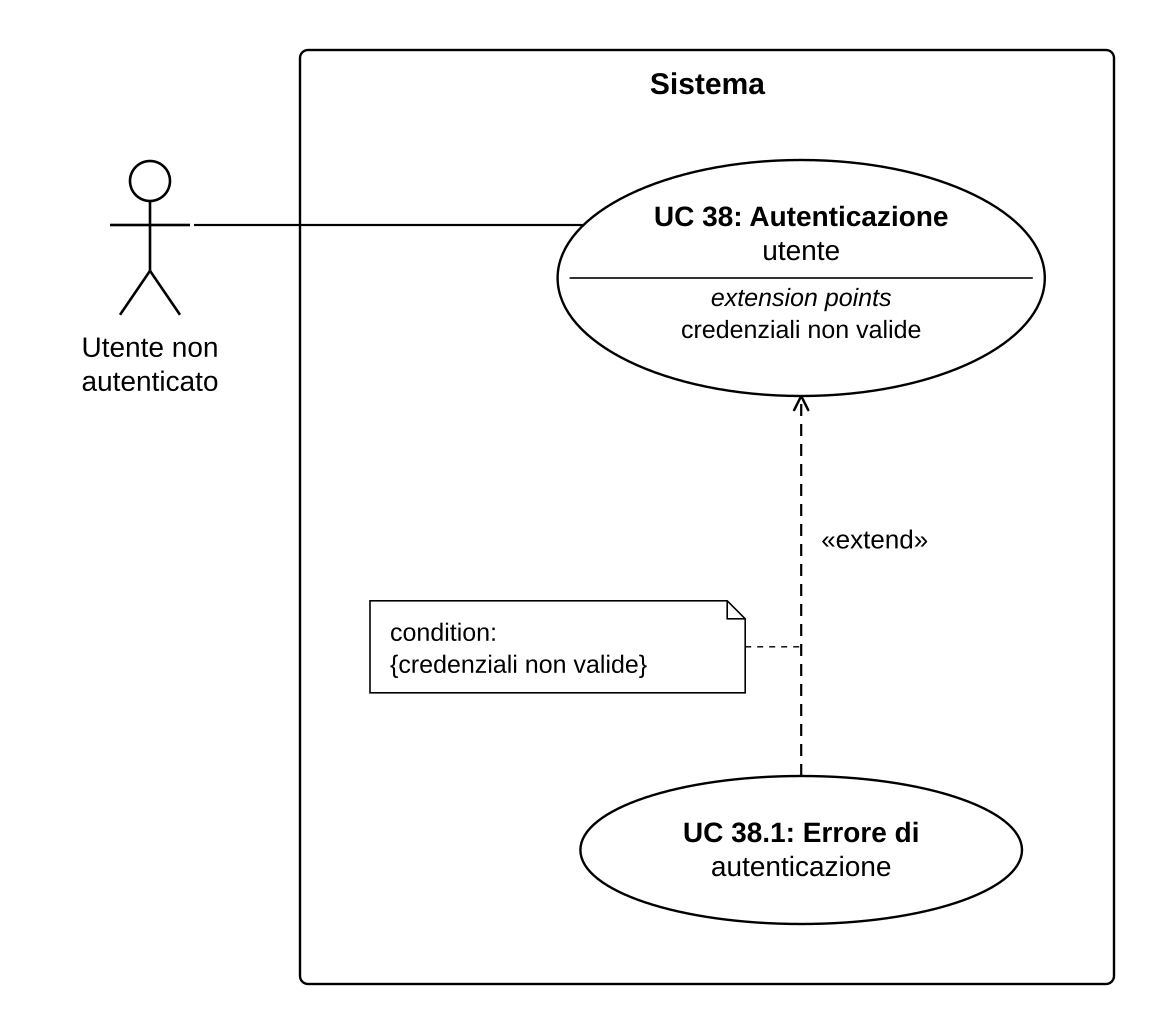
\includegraphics[width=\linewidth,height=0.32\textheight,keepaspectratio]{img/UC38.png}
\caption{UC 38 -- Autenticazione utente}
\end{center}
\begin{itemize}
    \item \textbf{Attore principale}: Utente non autenticato
    \item \textbf{Precondizioni}: L'utente possiede un account e non è autenticato.
    \item \textbf{Scenario principale}:
    \begin{enumerate}
        \item L'utente apre l'interfaccia amministrativa.
        \item Il sistema mostra il modulo di autenticazione.
        \item L'utente inserisce le credenziali.
        \item Il sistema verifica le credenziali e abilita l'accesso con il profilo dell'utente.
    \end{enumerate}
    \item \textbf{Postcondizioni}: L'utente è autenticato.
    \item \textbf{Trigger}: L'utente vuole accedere all'interfaccia amministrativa.
    \item \textbf{Estensioni}:
    \begin{itemize}
        \item \hyperref[uc:38.1]{UC 38.1}: Errore di autenticazione $\rightarrow$ Condizione: Credenziali non valide.
    \end{itemize}
\end{itemize}

\subsubsection{UC 38.1: Errore di autenticazione}\label{uc:38.1}
\begin{center}
\captionsetup{type=figure}
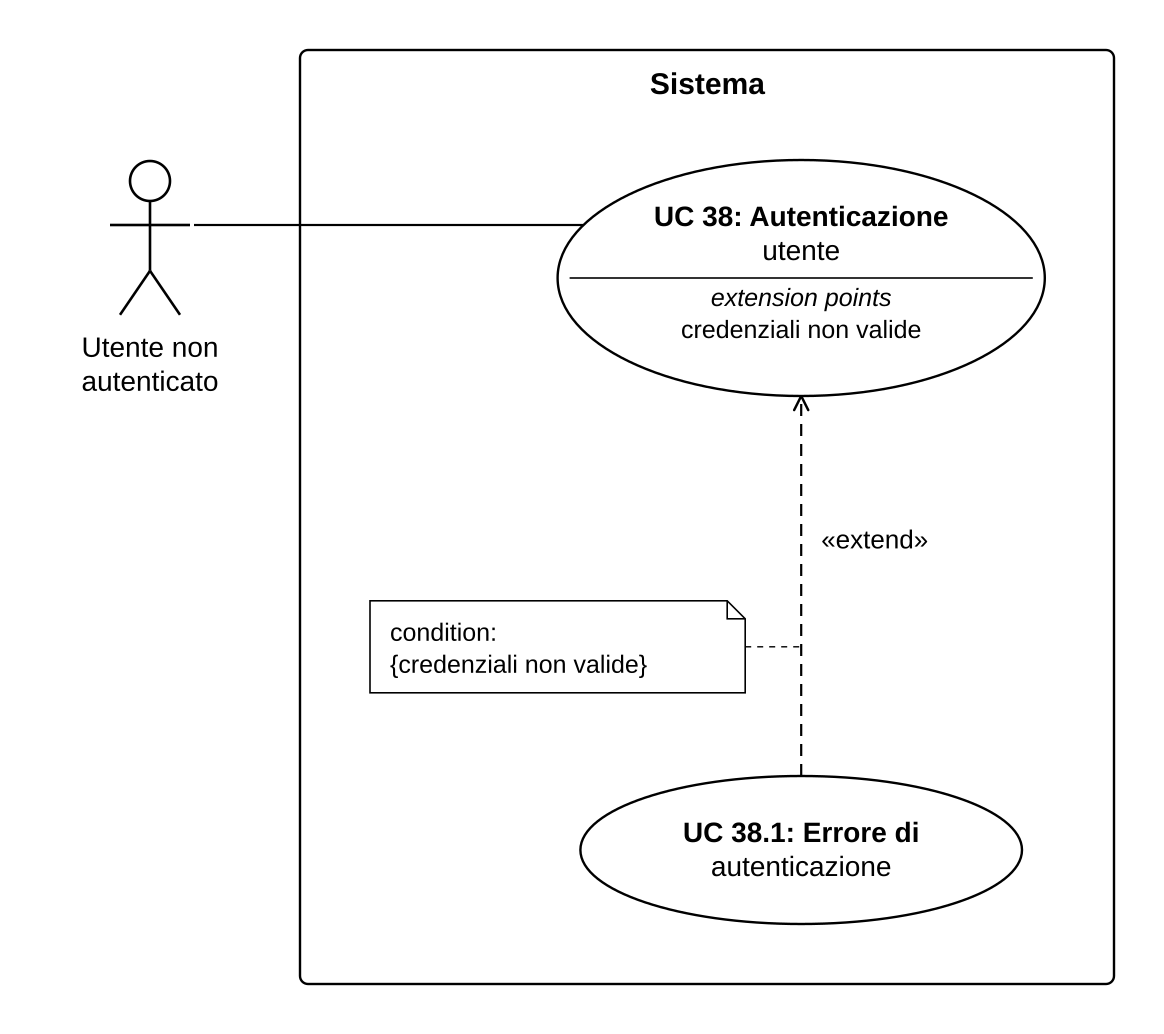
\includegraphics[width=\linewidth,height=0.32\textheight,keepaspectratio]{img/UC38_1.png}
\caption{UC 38.1 -- Errore di autenticazione}
\end{center}
\begin{itemize}
    \item \textbf{Attore principale}: Utente non autenticato
    \item \textbf{Precondizioni}: L'autenticazione è in corso.
    \item \textbf{Scenario principale}:
    \begin{enumerate}
        \item Il sistema rileva credenziali non valide.
        \item Il sistema segnala all'utente il fallimento dell'autenticazione.
    \end{enumerate}
    \item \textbf{Postcondizioni}: L'utente non è autenticato.
    \item \textbf{Trigger}: Inserimento di credenziali non valide.
    \item \textbf{Estende}: \hyperref[uc:38]{UC 38}.
\end{itemize}

\subsubsection{UC 39: Logout utente}\label{uc:39}
\begin{center}
\captionsetup{type=figure}
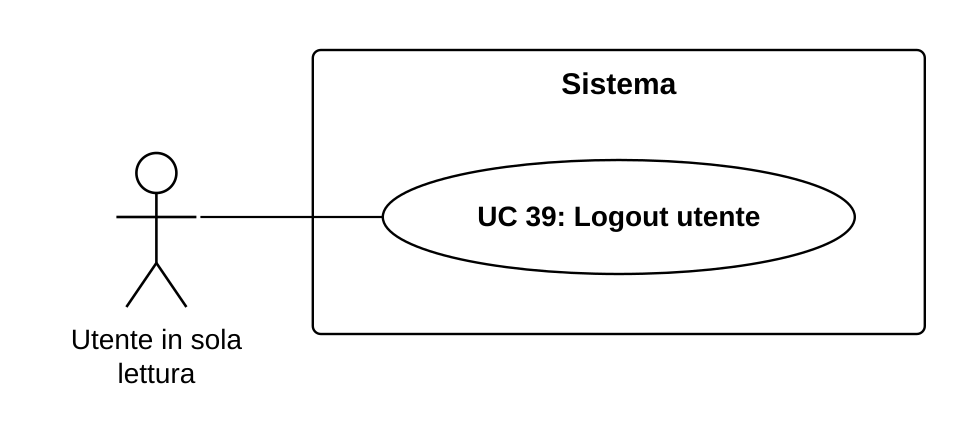
\includegraphics[width=\linewidth,height=0.32\textheight,keepaspectratio]{img/UC39.png}
\caption{UC 39 -- Logout utente}
\end{center}
\begin{itemize}
    \item \textbf{Attore principale}: Utente in sola lettura
    \item \textbf{Precondizioni}: L'utente è autenticato.
    \item \textbf{Scenario principale}:
    \begin{enumerate}
        \item L'utente attiva il comando di logout.
        \item Il sistema termina la sessione.
    \end{enumerate}
    \item \textbf{Postcondizioni}: La sessione è terminata.
    \item \textbf{Trigger}: L'utente vuole uscire dall'interfaccia.
\end{itemize}

\subsubsection{UC 40: Creazione di un utente con profilo di accesso}\label{uc:40}
\begin{center}
\captionsetup{type=figure}
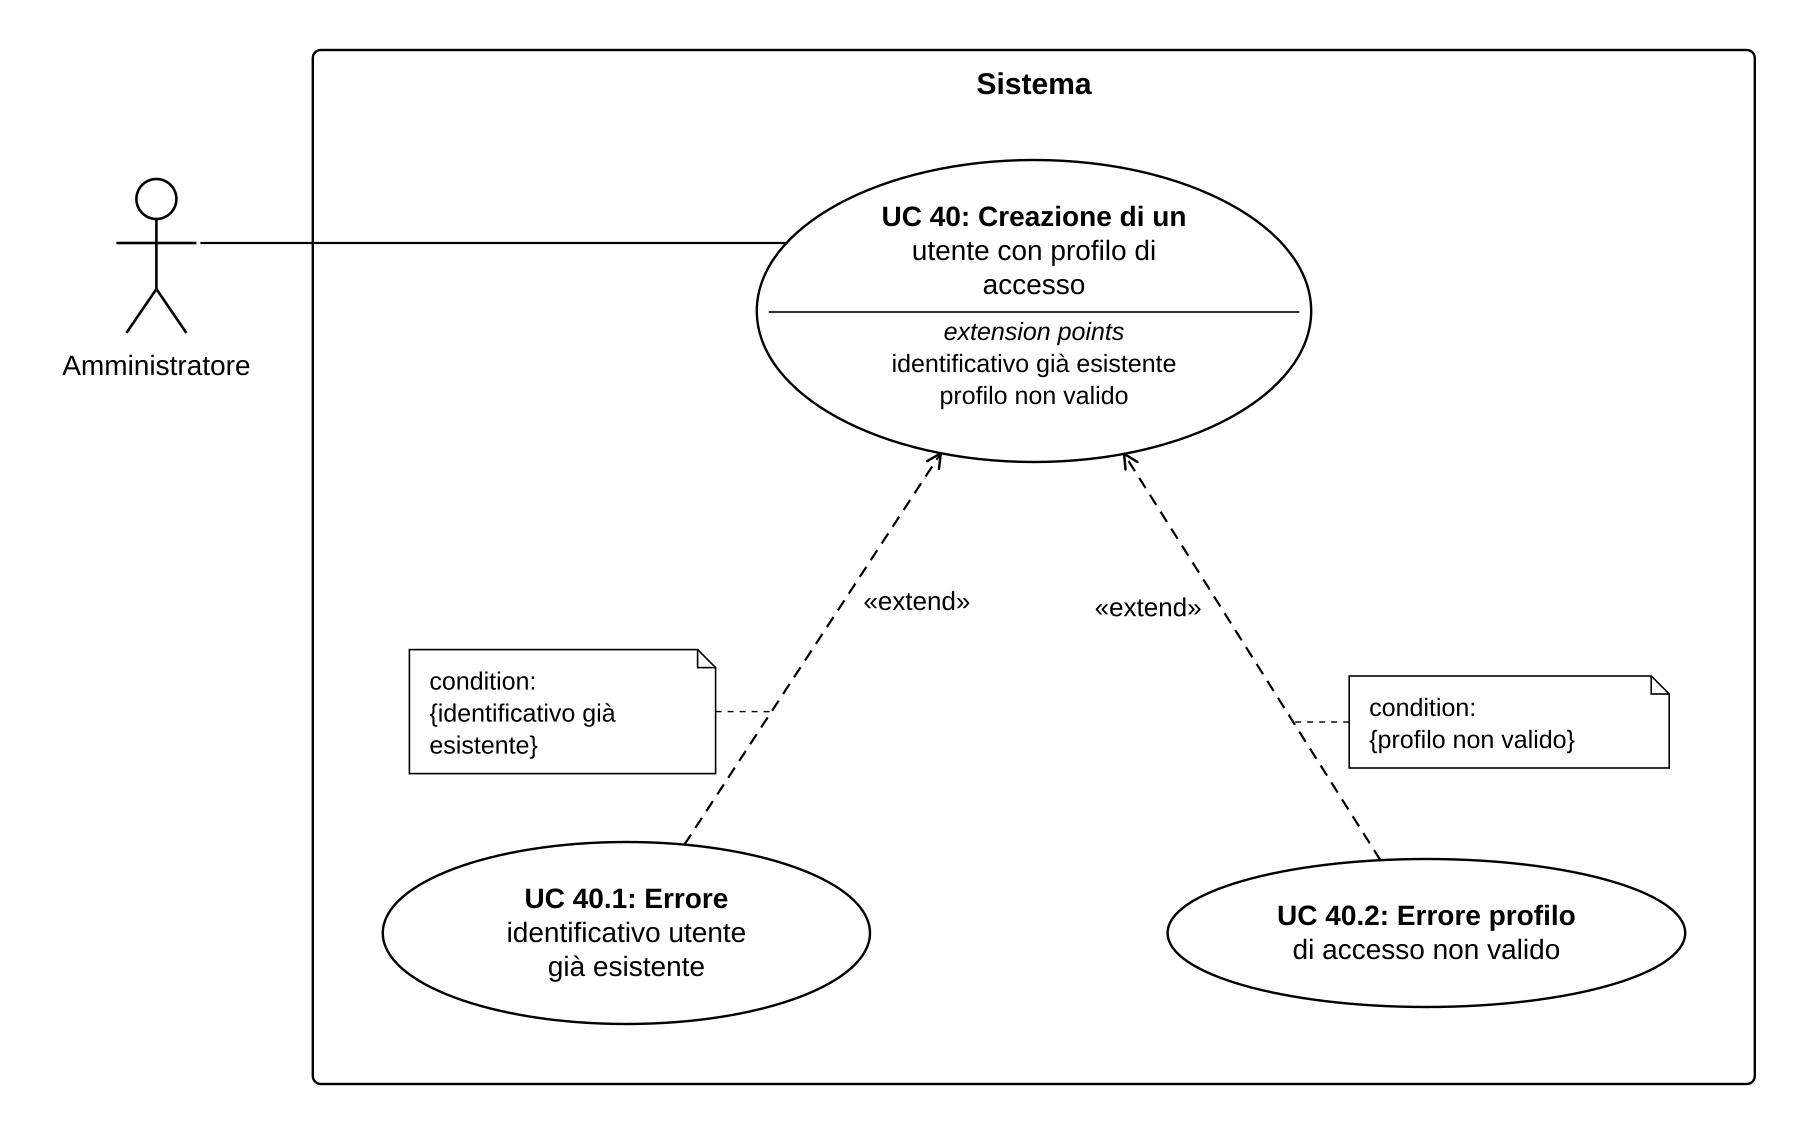
\includegraphics[width=\linewidth,height=0.32\textheight,keepaspectratio]{img/UC40.png}
\caption{UC 40 -- Creazione di un utente con profilo di accesso}
\end{center}
\begin{itemize}
    \item \textbf{Attore principale}: Amministratore
    \item \textbf{Precondizioni}: L'Amministratore è autenticato.
    \item \textbf{Scenario principale}:
    \begin{enumerate}
        \item L'Amministratore seleziona la creazione di un utente.
        \item L'Amministratore inserisce l'identificativo e sceglie il profilo di accesso.
        \item Il sistema valida i dati e crea l'utente.
    \end{enumerate}
    \item \textbf{Postcondizioni}: L'utente è creato con il profilo assegnato.
    \item \textbf{Trigger}: L'Amministratore vuole creare un utente.
    \item \textbf{Estensioni}:
    \begin{itemize}
        \item \hyperref[uc:40.1]{UC 40.1}: Errore identificativo utente già esistente $\rightarrow$ Condizione: Identificativo già esistente.
        \item \hyperref[uc:40.2]{UC 40.2}: Errore profilo di accesso non valido $\rightarrow$ Condizione: Profilo non valido.
    \end{itemize}
\end{itemize}

\subsubsection{UC 40.1: Errore identificativo utente già esistente}\label{uc:40.1}
\begin{center}
\captionsetup{type=figure}
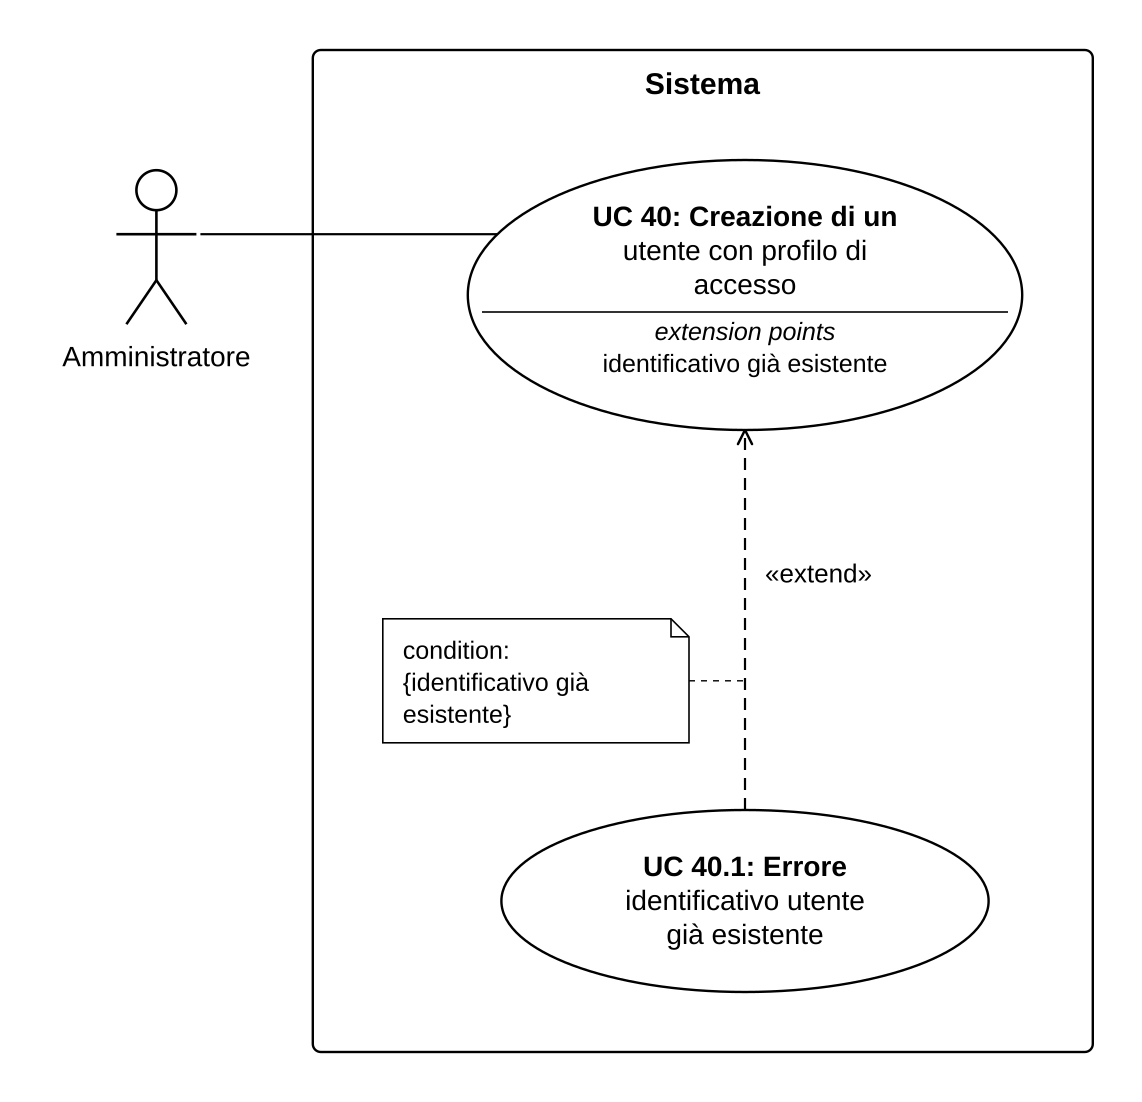
\includegraphics[width=\linewidth,height=0.32\textheight,keepaspectratio]{img/UC40_1.png}
\caption{UC 40.1 -- Errore identificativo utente già esistente}
\end{center}
\begin{itemize}
    \item \textbf{Attore principale}: Amministratore
    \item \textbf{Precondizioni}: La creazione di un utente è in corso.
    \item \textbf{Scenario principale}:
    \begin{enumerate}
        \item Il sistema rileva che l'identificativo esiste già.
        \item Il sistema segnala l'errore all'Amministratore.
    \end{enumerate}
    \item \textbf{Postcondizioni}: Nessun utente è creato.
    \item \textbf{Trigger}: Identificativo già esistente.
    \item \textbf{Estende}: \hyperref[uc:40]{UC 40}.
\end{itemize}

\subsubsection{UC 40.2: Errore profilo di accesso non valido}\label{uc:40.2}
\begin{center}
\captionsetup{type=figure}
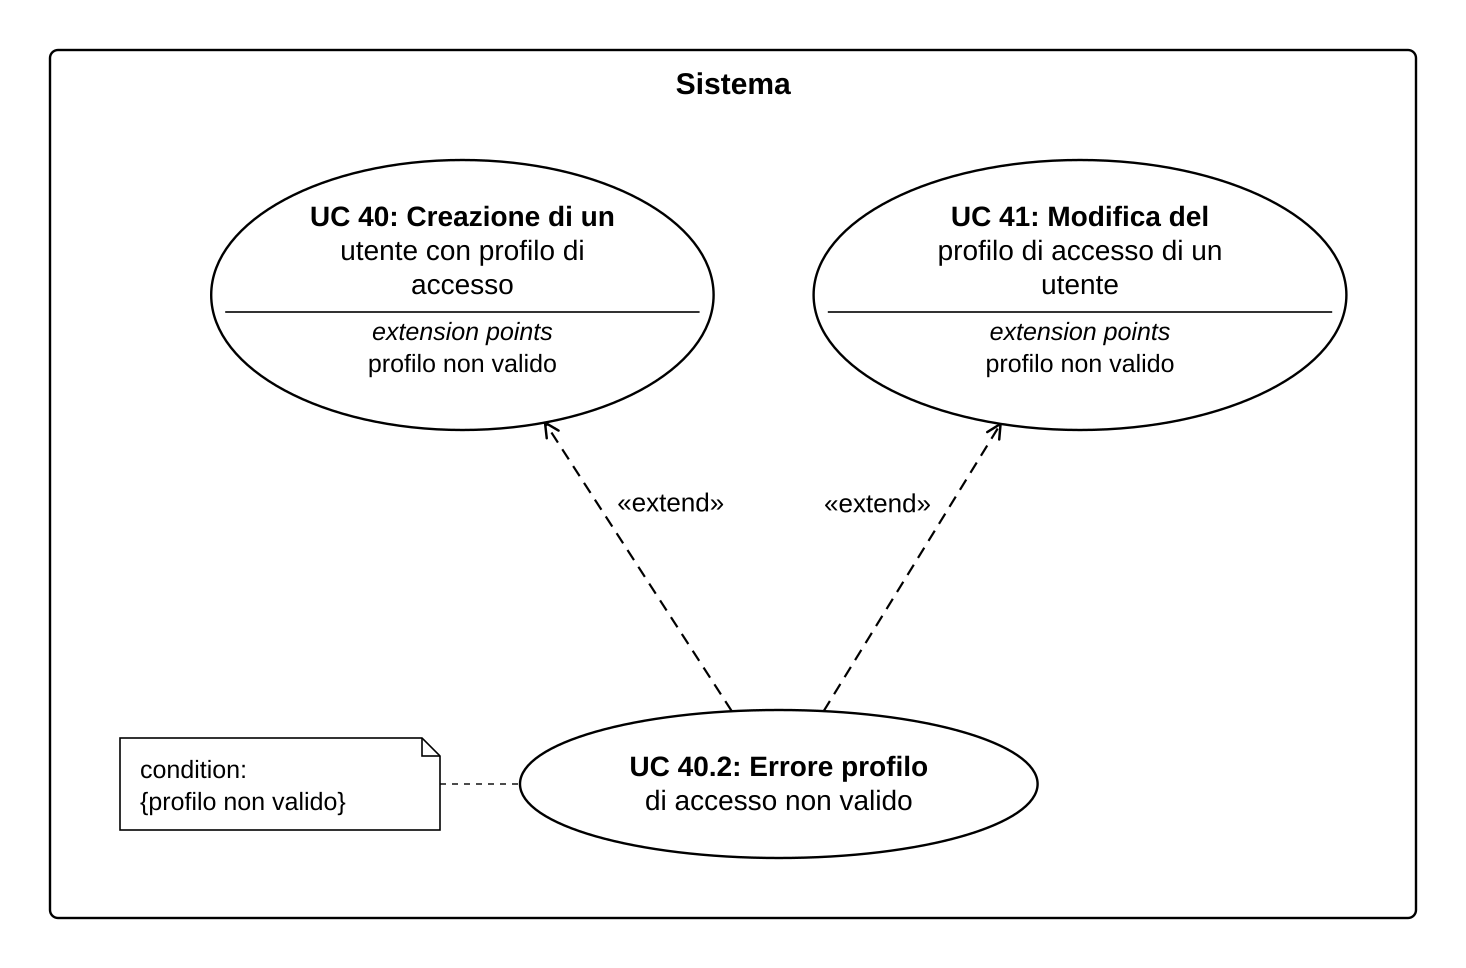
\includegraphics[width=\linewidth,height=0.32\textheight,keepaspectratio]{img/UC40_2.png}
\caption{UC 40.2 -- Errore profilo di accesso non valido}
\end{center}
\begin{itemize}
    \item \textbf{Attore principale}: Amministratore
    \item \textbf{Precondizioni}: La gestione di un utente è in corso.
    \item \textbf{Scenario principale}:
    \begin{enumerate}
        \item Il sistema rileva che il profilo indicato non è valido.
        \item Il sistema segnala l'errore all'Amministratore.
    \end{enumerate}
    \item \textbf{Postcondizioni}: Nessuna modifica è applicata.
    \item \textbf{Trigger}: Profilo di accesso non valido.
    \item \textbf{Estende}: \hyperref[uc:40]{UC 40}, \hyperref[uc:41]{UC 41}.
\end{itemize}

\subsubsection{UC 41: Modifica del profilo di accesso di un utente}\label{uc:41}
\begin{center}
\captionsetup{type=figure}
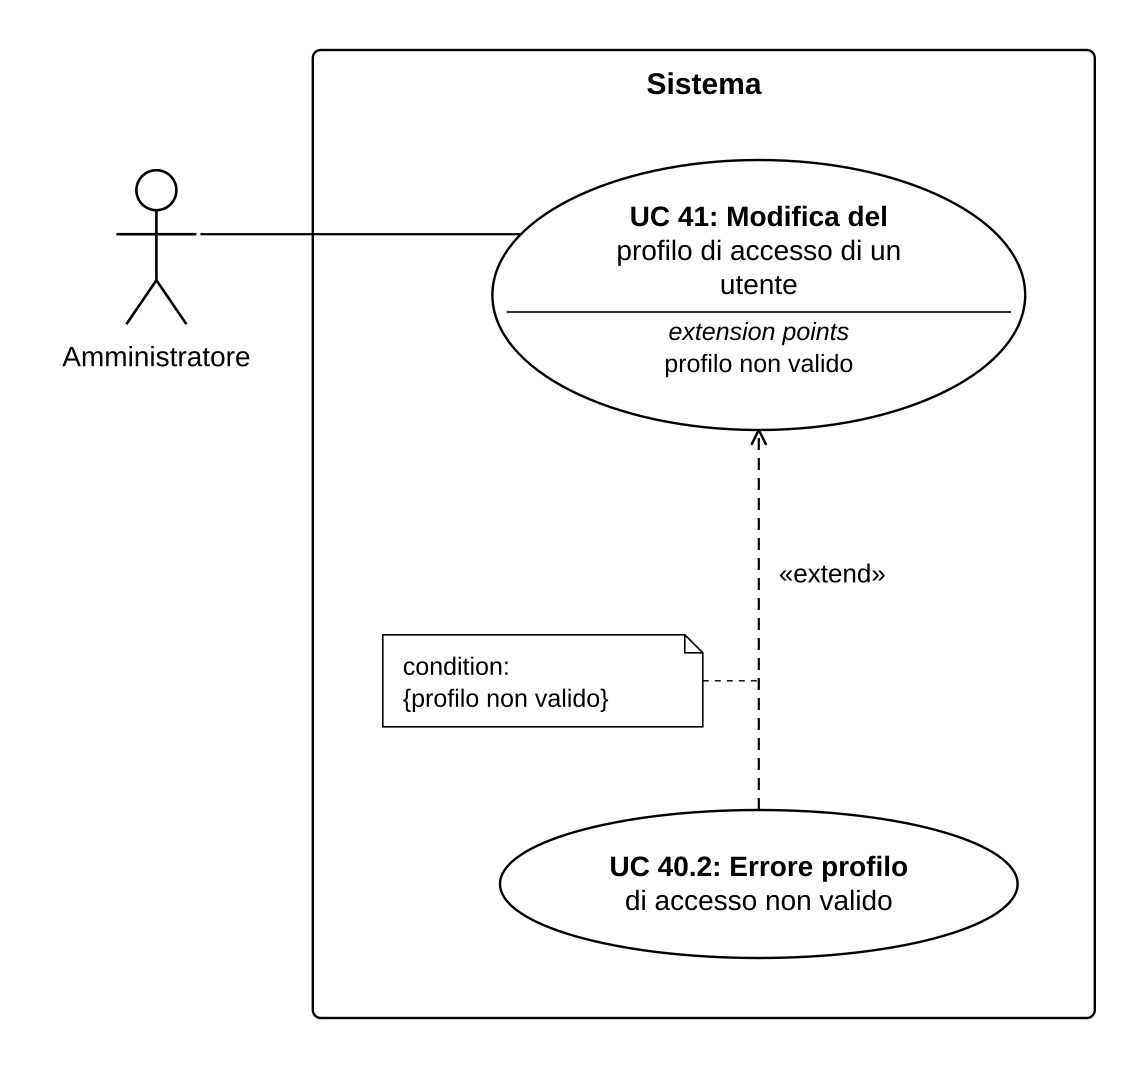
\includegraphics[width=\linewidth,height=0.32\textheight,keepaspectratio]{img/UC41.png}
\caption{UC 41 -- Modifica del profilo di accesso di un utente}
\end{center}
\begin{itemize}
    \item \textbf{Attore principale}: Amministratore
    \item \textbf{Precondizioni}: L'Amministratore è autenticato ed esiste almeno un utente.
    \item \textbf{Scenario principale}:
    \begin{enumerate}
        \item L'Amministratore seleziona un utente.
        \item L'Amministratore sceglie un nuovo profilo di accesso.
        \item Il sistema valida e salva la modifica.
    \end{enumerate}
    \item \textbf{Postcondizioni}: Il profilo dell'utente è aggiornato.
    \item \textbf{Trigger}: L'Amministratore vuole modificare il profilo di un utente.
    \item \textbf{Estensioni}:
    \begin{itemize}
        \item \hyperref[uc:40.2]{UC 40.2}: Errore profilo di accesso non valido $\rightarrow$ Condizione: Profilo non valido.
    \end{itemize}
\end{itemize}

\subsubsection{UC 42: Rimozione di un utente}\label{uc:42}
\begin{center}
\captionsetup{type=figure}
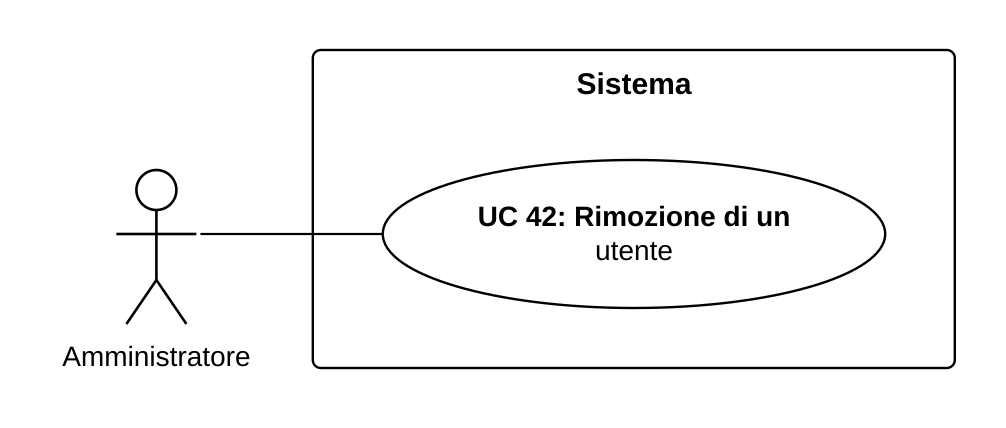
\includegraphics[width=\linewidth,height=0.32\textheight,keepaspectratio]{img/UC42.png}
\caption{UC 42 -- Rimozione di un utente}
\end{center}
\begin{itemize}
    \item \textbf{Attore principale}: Amministratore
    \item \textbf{Precondizioni}: L'Amministratore è autenticato ed esiste almeno un utente.
    \item \textbf{Scenario principale}:
    \begin{enumerate}
        \item L'Amministratore seleziona un utente.
        \item L'Amministratore richiede la rimozione.
        \item Il sistema rimuove l'utente.
    \end{enumerate}
    \item \textbf{Postcondizioni}: L'utente è rimosso.
    \item \textbf{Trigger}: L'Amministratore vuole rimuovere un utente.
\end{itemize}

\subsubsection{UC 43: Visualizzazione dei canali di ingresso e del loro stato}\label{uc:43}
\begin{center}
\captionsetup{type=figure}
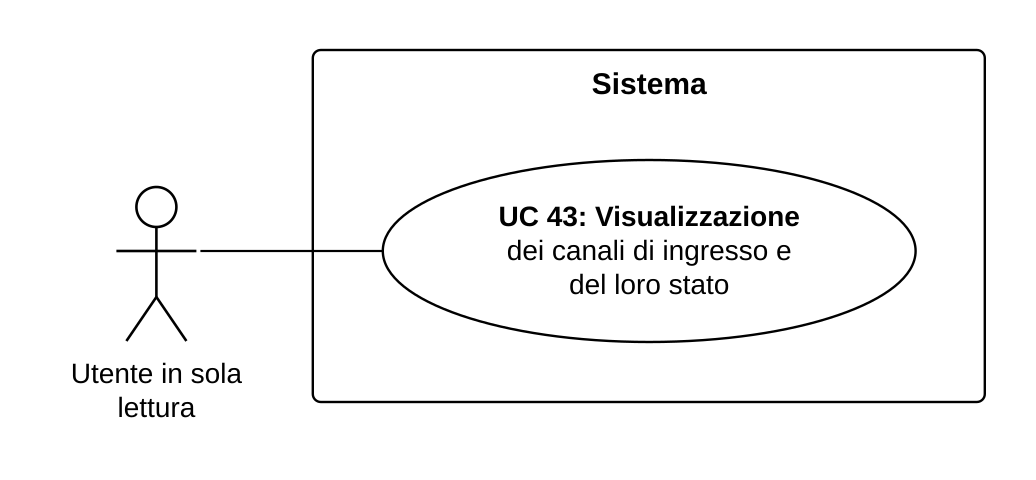
\includegraphics[width=\linewidth,height=0.32\textheight,keepaspectratio]{img/UC43.png}
\caption{UC 43 -- Visualizzazione dei canali di ingresso e del loro stato}
\end{center}
\begin{itemize}
    \item \textbf{Attore principale}: Utente in sola lettura
    \item \textbf{Precondizioni}: L'utente è autenticato.
    \item \textbf{Scenario principale}:
    \begin{enumerate}
        \item L'utente apre la sezione dei canali.
        \item Il sistema mostra i canali configurati e il loro stato.
    \end{enumerate}
    \item \textbf{Postcondizioni}: I canali e il loro stato sono visualizzati.
    \item \textbf{Trigger}: L'utente vuole conoscere i canali configurati.
\end{itemize}

\subsubsection{UC 44: Configurazione di un nuovo canale di ingresso}\label{uc:44}
\begin{center}
\captionsetup{type=figure}
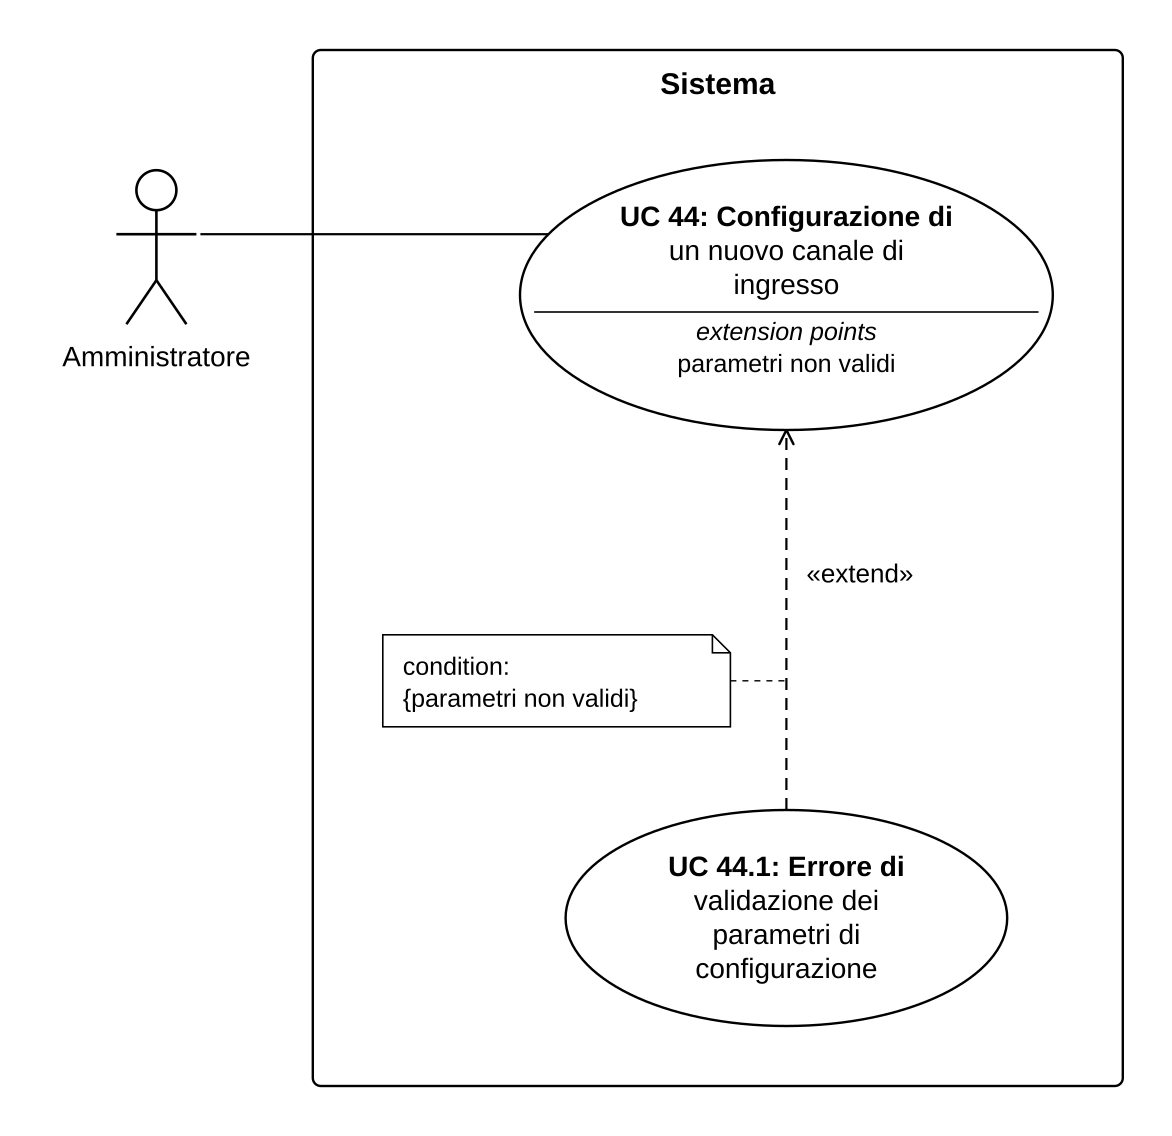
\includegraphics[width=\linewidth,height=0.32\textheight,keepaspectratio]{img/UC44.png}
\caption{UC 44 -- Configurazione di un nuovo canale di ingresso}
\end{center}
\begin{itemize}
    \item \textbf{Attore principale}: Amministratore
    \item \textbf{Precondizioni}: L'Amministratore è autenticato.
    \item \textbf{Scenario principale}:
    \begin{enumerate}
        \item L'Amministratore seleziona la configurazione di un nuovo canale.
        \item L'Amministratore inserisce tipo e parametri del canale.
        \item Il sistema valida i parametri e salva la configurazione.
    \end{enumerate}
    \item \textbf{Postcondizioni}: Il nuovo canale è configurato.
    \item \textbf{Trigger}: L'Amministratore vuole aggiungere un canale di ingresso.
    \item \textbf{Estensioni}:
    \begin{itemize}
        \item \hyperref[uc:44.1]{UC 44.1}: Errore di validazione dei parametri di configurazione $\rightarrow$ Condizione: Parametri non validi.
    \end{itemize}
\end{itemize}

\subsubsection{UC 44.1: Errore di validazione dei parametri di configurazione}\label{uc:44.1}
\begin{center}
\captionsetup{type=figure}
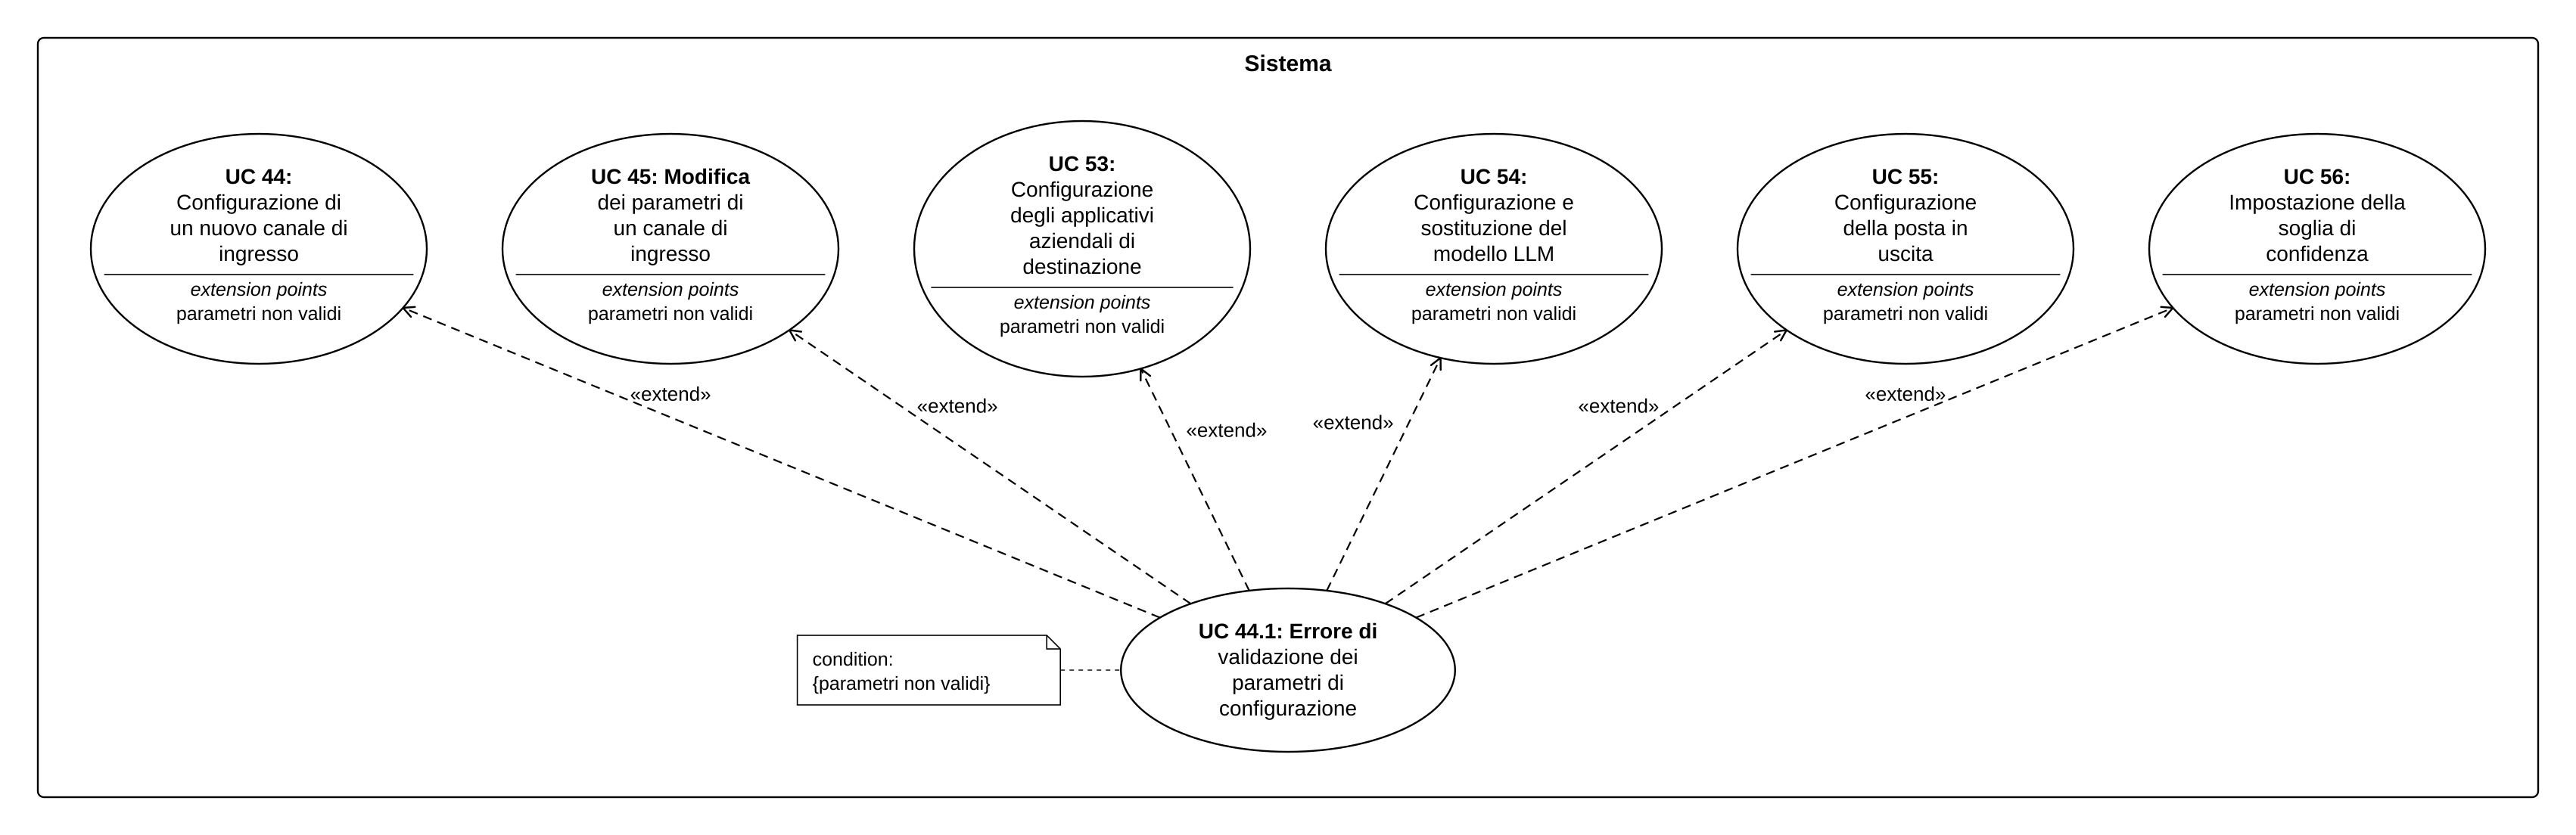
\includegraphics[width=\linewidth,height=0.32\textheight,keepaspectratio]{img/UC44_1.png}
\caption{UC 44.1 -- Errore di validazione dei parametri di configurazione}
\end{center}
\begin{itemize}
    \item \textbf{Attore principale}: Amministratore
    \item \textbf{Precondizioni}: Una configurazione è in corso di salvataggio.
    \item \textbf{Scenario principale}:
    \begin{enumerate}
        \item Il sistema rileva parametri non validi.
        \item Il sistema segnala gli errori di validazione all'utente.
        \item Il sistema non salva la configurazione.
    \end{enumerate}
    \item \textbf{Postcondizioni}: La configurazione non è salvata.
    \item \textbf{Trigger}: Parametri di configurazione non validi.
    \item \textbf{Estende}: \hyperref[uc:44]{UC 44}, \hyperref[uc:45]{UC 45}, \hyperref[uc:53]{UC 53}, \hyperref[uc:54]{UC 54}, \hyperref[uc:55]{UC 55}, \hyperref[uc:56]{UC 56}.
\end{itemize}

\subsubsection{UC 45: Modifica dei parametri di un canale di ingresso}\label{uc:45}
\begin{center}
\captionsetup{type=figure}
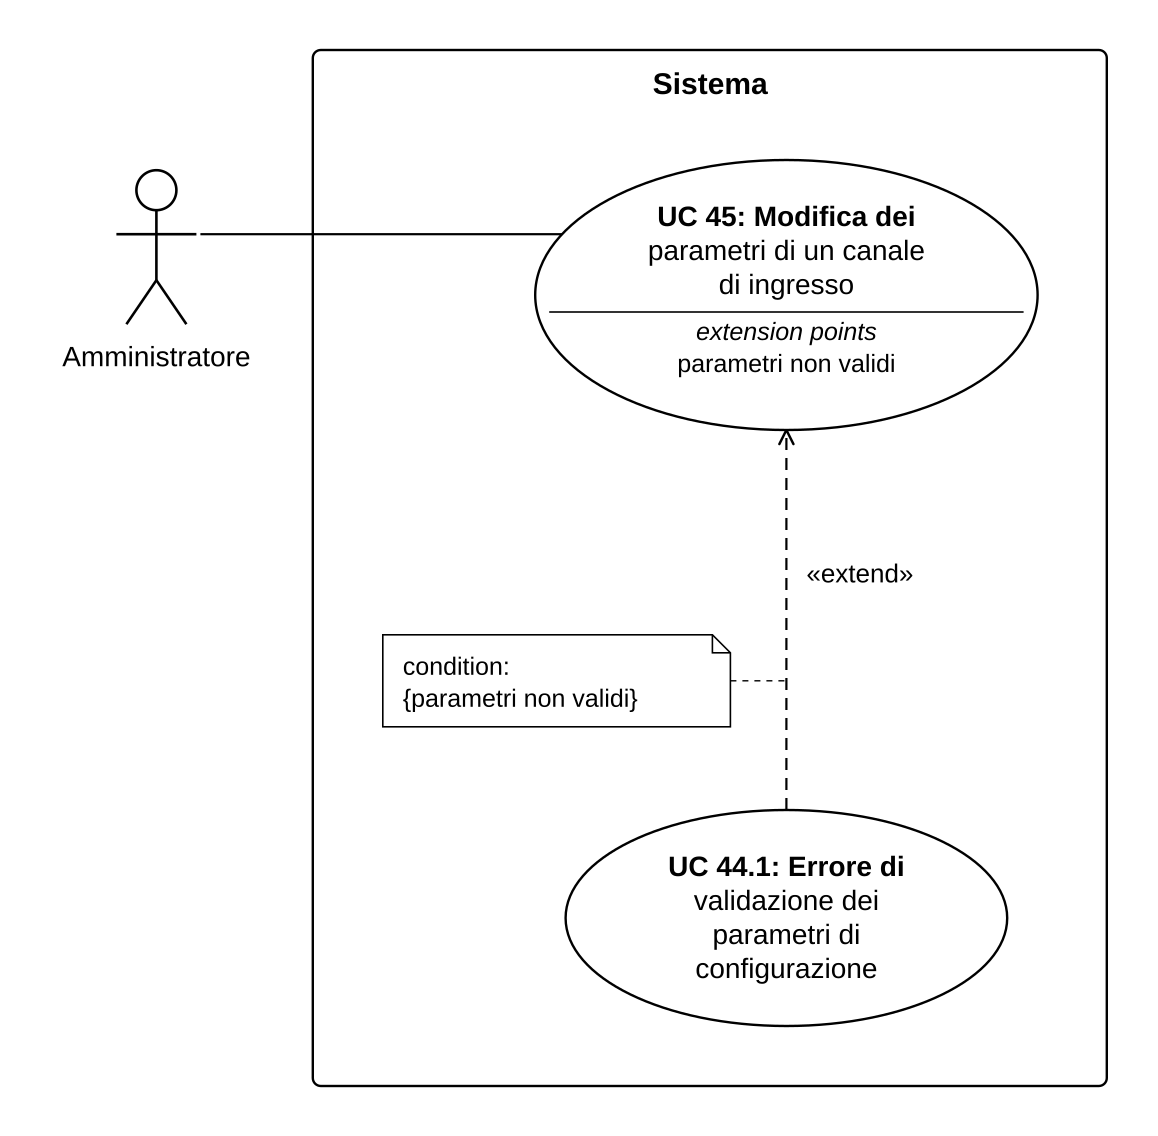
\includegraphics[width=\linewidth,height=0.32\textheight,keepaspectratio]{img/UC45.png}
\caption{UC 45 -- Modifica dei parametri di un canale di ingresso}
\end{center}
\begin{itemize}
    \item \textbf{Attore principale}: Amministratore
    \item \textbf{Precondizioni}: L'Amministratore è autenticato ed esiste almeno un canale.
    \item \textbf{Scenario principale}:
    \begin{enumerate}
        \item L'Amministratore seleziona un canale.
        \item L'Amministratore modifica i parametri.
        \item Il sistema valida i parametri e salva la configurazione.
    \end{enumerate}
    \item \textbf{Postcondizioni}: I parametri del canale sono aggiornati.
    \item \textbf{Trigger}: L'Amministratore vuole modificare un canale.
    \item \textbf{Estensioni}:
    \begin{itemize}
        \item \hyperref[uc:44.1]{UC 44.1}: Errore di validazione dei parametri di configurazione $\rightarrow$ Condizione: Parametri non validi.
    \end{itemize}
\end{itemize}

\subsubsection{UC 46: Rimozione di un canale di ingresso}\label{uc:46}
\begin{center}
\captionsetup{type=figure}
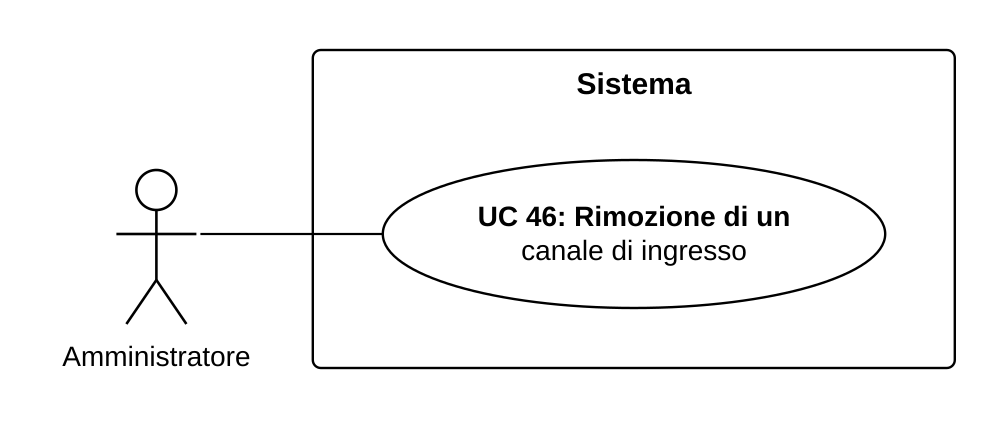
\includegraphics[width=\linewidth,height=0.32\textheight,keepaspectratio]{img/UC46.png}
\caption{UC 46 -- Rimozione di un canale di ingresso}
\end{center}
\begin{itemize}
    \item \textbf{Attore principale}: Amministratore
    \item \textbf{Precondizioni}: L'Amministratore è autenticato ed esiste almeno un canale.
    \item \textbf{Scenario principale}:
    \begin{enumerate}
        \item L'Amministratore seleziona un canale.
        \item L'Amministratore richiede la rimozione.
        \item Il sistema rimuove il canale.
    \end{enumerate}
    \item \textbf{Postcondizioni}: Il canale è rimosso.
    \item \textbf{Trigger}: L'Amministratore vuole rimuovere un canale.
\end{itemize}

\subsubsection{UC 47: Attivazione di un canale di ingresso}\label{uc:47}
\begin{center}
\captionsetup{type=figure}
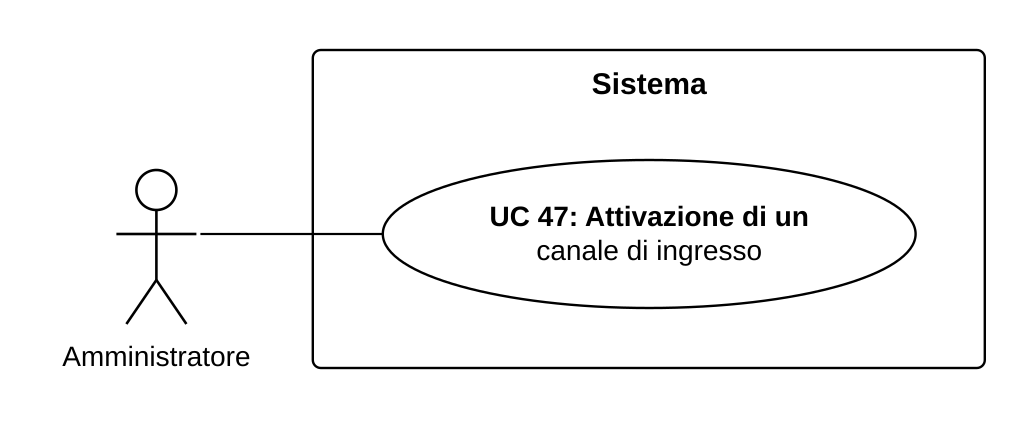
\includegraphics[width=\linewidth,height=0.32\textheight,keepaspectratio]{img/UC47.png}
\caption{UC 47 -- Attivazione di un canale di ingresso}
\end{center}
\begin{itemize}
    \item \textbf{Attore principale}: Amministratore
    \item \textbf{Precondizioni}: L'Amministratore è autenticato ed esiste un canale disattivato.
    \item \textbf{Scenario principale}:
    \begin{enumerate}
        \item L'Amministratore seleziona il canale.
        \item L'Amministratore attiva il canale.
        \item Il sistema riprende il monitoraggio del canale.
    \end{enumerate}
    \item \textbf{Postcondizioni}: Il canale è attivo.
    \item \textbf{Trigger}: L'Amministratore vuole attivare un canale.
\end{itemize}

\subsubsection{UC 48: Disattivazione di un canale di ingresso}\label{uc:48}
\begin{center}
\captionsetup{type=figure}
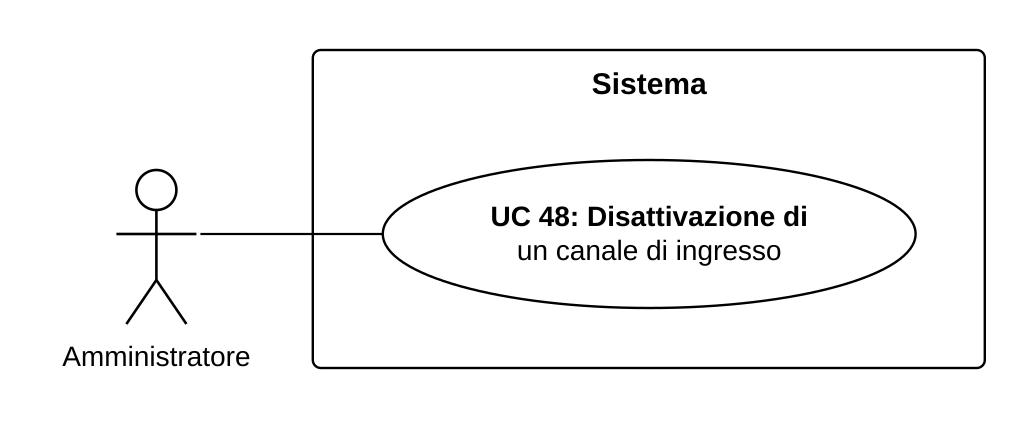
\includegraphics[width=\linewidth,height=0.32\textheight,keepaspectratio]{img/UC48.png}
\caption{UC 48 -- Disattivazione di un canale di ingresso}
\end{center}
\begin{itemize}
    \item \textbf{Attore principale}: Amministratore
    \item \textbf{Precondizioni}: L'Amministratore è autenticato ed esiste un canale attivo.
    \item \textbf{Scenario principale}:
    \begin{enumerate}
        \item L'Amministratore seleziona il canale.
        \item L'Amministratore disattiva il canale.
        \item Il sistema sospende il monitoraggio del canale.
    \end{enumerate}
    \item \textbf{Postcondizioni}: Il canale è disattivato.
    \item \textbf{Trigger}: L'Amministratore vuole disattivare un canale.
\end{itemize}

\subsubsection{UC 49: Visualizzazione delle regole di azione e notifica}\label{uc:49}
\begin{center}
\captionsetup{type=figure}
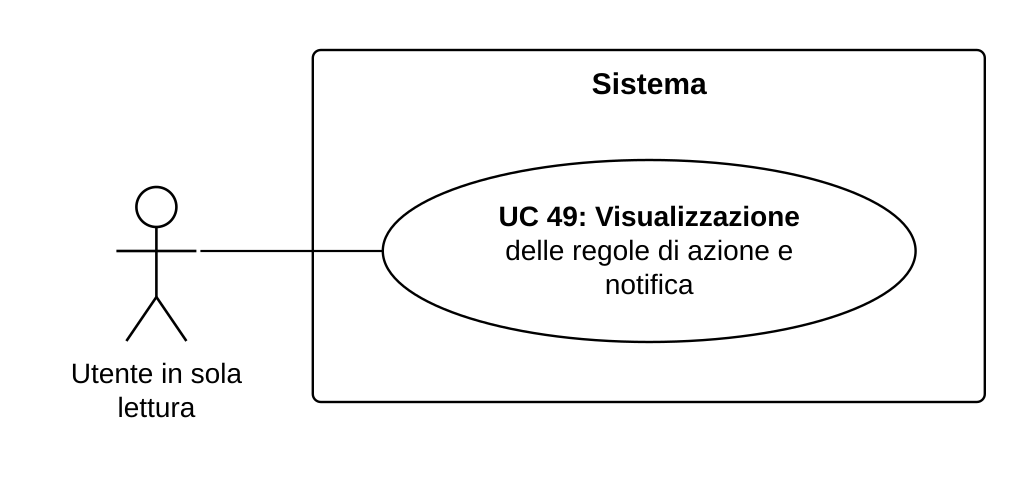
\includegraphics[width=\linewidth,height=0.32\textheight,keepaspectratio]{img/UC49.png}
\caption{UC 49 -- Visualizzazione delle regole di azione e notifica}
\end{center}
\begin{itemize}
    \item \textbf{Attore principale}: Utente in sola lettura
    \item \textbf{Precondizioni}: L'utente è autenticato.
    \item \textbf{Scenario principale}:
    \begin{enumerate}
        \item L'utente apre la sezione delle regole.
        \item Il sistema mostra le regole di azione e notifica configurate.
    \end{enumerate}
    \item \textbf{Postcondizioni}: Le regole sono visualizzate.
    \item \textbf{Trigger}: L'utente vuole consultare le regole.
\end{itemize}

\subsubsection{UC 50: Creazione di una regola di azione o notifica}\label{uc:50}
\begin{center}
\captionsetup{type=figure}
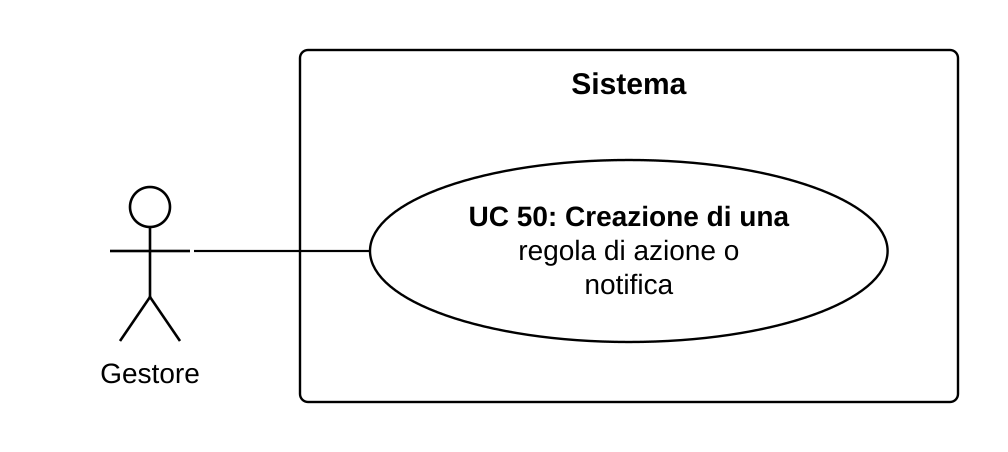
\includegraphics[width=\linewidth,height=0.32\textheight,keepaspectratio]{img/UC50.png}
\caption{UC 50 -- Creazione di una regola di azione o notifica}
\end{center}
\begin{itemize}
    \item \textbf{Attore principale}: Gestore
    \item \textbf{Precondizioni}: Il Gestore è autenticato.
    \item \textbf{Scenario principale}:
    \begin{enumerate}
        \item Il Gestore seleziona la creazione di una regola.
        \item Il Gestore associa una tipologia di richiesta a un'azione API REST o e-mail.
        \item Il sistema salva la regola.
    \end{enumerate}
    \item \textbf{Postcondizioni}: La regola è creata.
    \item \textbf{Trigger}: Il Gestore vuole definire una nuova regola.
\end{itemize}

\subsubsection{UC 51: Modifica di una regola di azione o notifica}\label{uc:51}
\begin{center}
\captionsetup{type=figure}
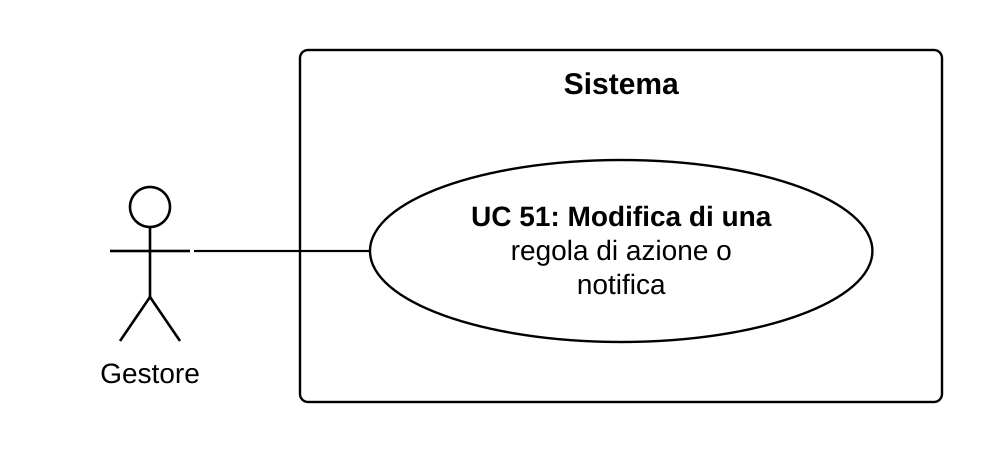
\includegraphics[width=\linewidth,height=0.32\textheight,keepaspectratio]{img/UC51.png}
\caption{UC 51 -- Modifica di una regola di azione o notifica}
\end{center}
\begin{itemize}
    \item \textbf{Attore principale}: Gestore
    \item \textbf{Precondizioni}: Il Gestore è autenticato ed esiste almeno una regola.
    \item \textbf{Scenario principale}:
    \begin{enumerate}
        \item Il Gestore seleziona una regola.
        \item Il Gestore ne modifica i parametri.
        \item Il sistema salva la modifica.
    \end{enumerate}
    \item \textbf{Postcondizioni}: La regola è aggiornata.
    \item \textbf{Trigger}: Il Gestore vuole modificare una regola.
\end{itemize}

\subsubsection{UC 52: Eliminazione di una regola di azione o notifica}\label{uc:52}
\begin{center}
\captionsetup{type=figure}
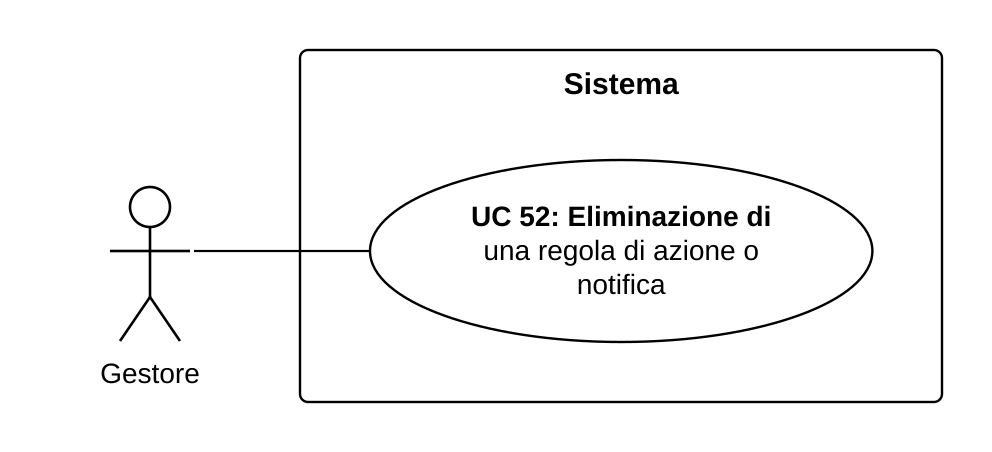
\includegraphics[width=\linewidth,height=0.32\textheight,keepaspectratio]{img/UC52.png}
\caption{UC 52 -- Eliminazione di una regola di azione o notifica}
\end{center}
\begin{itemize}
    \item \textbf{Attore principale}: Gestore
    \item \textbf{Precondizioni}: Il Gestore è autenticato ed esiste almeno una regola.
    \item \textbf{Scenario principale}:
    \begin{enumerate}
        \item Il Gestore seleziona una regola.
        \item Il Gestore richiede l'eliminazione.
        \item Il sistema elimina la regola.
    \end{enumerate}
    \item \textbf{Postcondizioni}: La regola è eliminata.
    \item \textbf{Trigger}: Il Gestore vuole eliminare una regola.
\end{itemize}

\subsubsection{UC 53: Configurazione degli applicativi aziendali di destinazione}\label{uc:53}
\begin{center}
\captionsetup{type=figure}
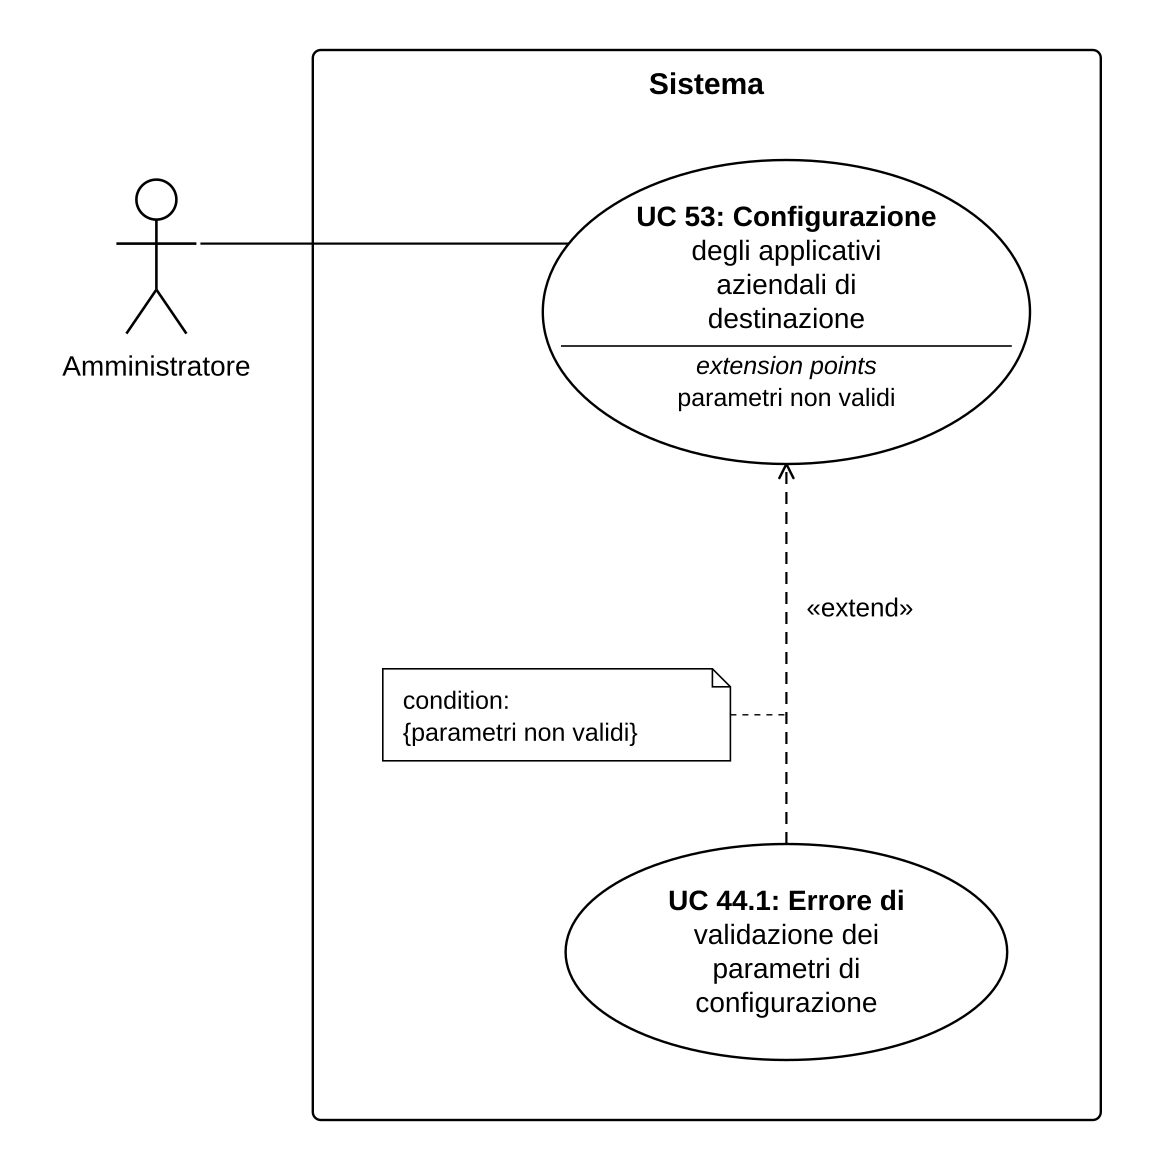
\includegraphics[width=\linewidth,height=0.32\textheight,keepaspectratio]{img/UC53.png}
\caption{UC 53 -- Configurazione degli applicativi aziendali di destinazione}
\end{center}
\begin{itemize}
    \item \textbf{Attore principale}: Amministratore
    \item \textbf{Precondizioni}: L'Amministratore è autenticato.
    \item \textbf{Scenario principale}:
    \begin{enumerate}
        \item L'Amministratore seleziona la configurazione degli applicativi.
        \item L'Amministratore inserisce indirizzo dell'API, credenziali e tipo.
        \item Il sistema valida i parametri e salva la configurazione.
    \end{enumerate}
    \item \textbf{Postcondizioni}: L'applicativo di destinazione è configurato.
    \item \textbf{Trigger}: L'Amministratore vuole configurare un applicativo di destinazione.
    \item \textbf{Estensioni}:
    \begin{itemize}
        \item \hyperref[uc:44.1]{UC 44.1}: Errore di validazione dei parametri di configurazione $\rightarrow$ Condizione: Parametri non validi.
    \end{itemize}
\end{itemize}

\subsubsection{UC 54: Configurazione e sostituzione del modello LLM}\label{uc:54}
\begin{center}
\captionsetup{type=figure}
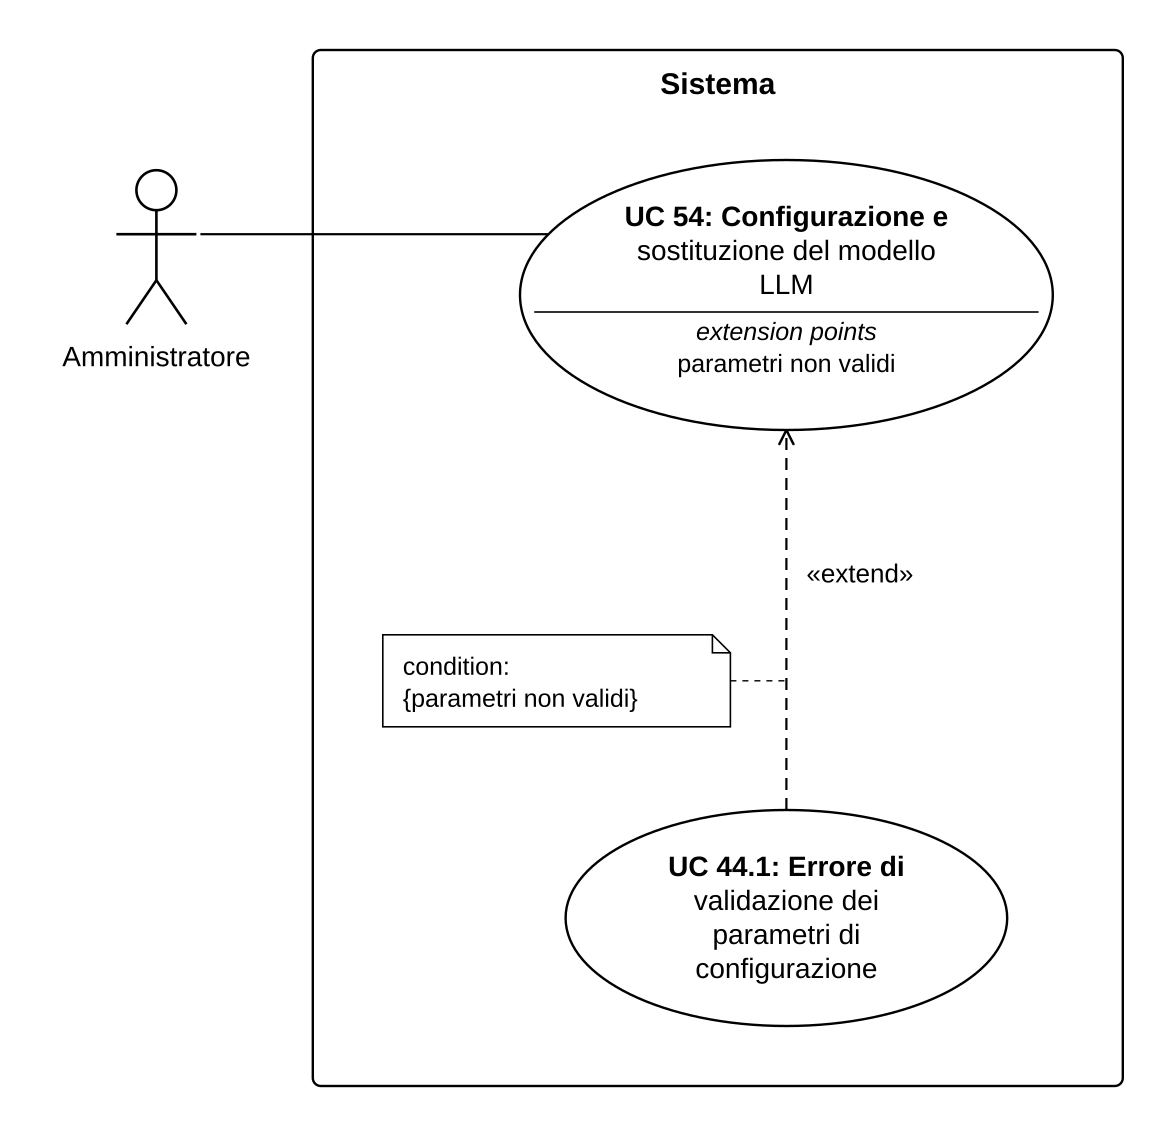
\includegraphics[width=\linewidth,height=0.32\textheight,keepaspectratio]{img/UC54.png}
\caption{UC 54 -- Configurazione e sostituzione del modello LLM}
\end{center}
\begin{itemize}
    \item \textbf{Attore principale}: Amministratore
    \item \textbf{Precondizioni}: L'Amministratore è autenticato.
    \item \textbf{Scenario principale}:
    \begin{enumerate}
        \item L'Amministratore seleziona la configurazione del modello LLM.
        \item L'Amministratore inserisce l'endpoint compatibile OpenAI e il nome del modello.
        \item Il sistema valida i parametri e salva la configurazione.
    \end{enumerate}
    \item \textbf{Postcondizioni}: Il modello LLM è configurato o sostituito.
    \item \textbf{Trigger}: L'Amministratore vuole configurare o sostituire il modello LLM.
    \item \textbf{Estensioni}:
    \begin{itemize}
        \item \hyperref[uc:44.1]{UC 44.1}: Errore di validazione dei parametri di configurazione $\rightarrow$ Condizione: Parametri non validi.
    \end{itemize}
\end{itemize}

\subsubsection{UC 55: Configurazione della posta in uscita}\label{uc:55}
\begin{center}
\captionsetup{type=figure}
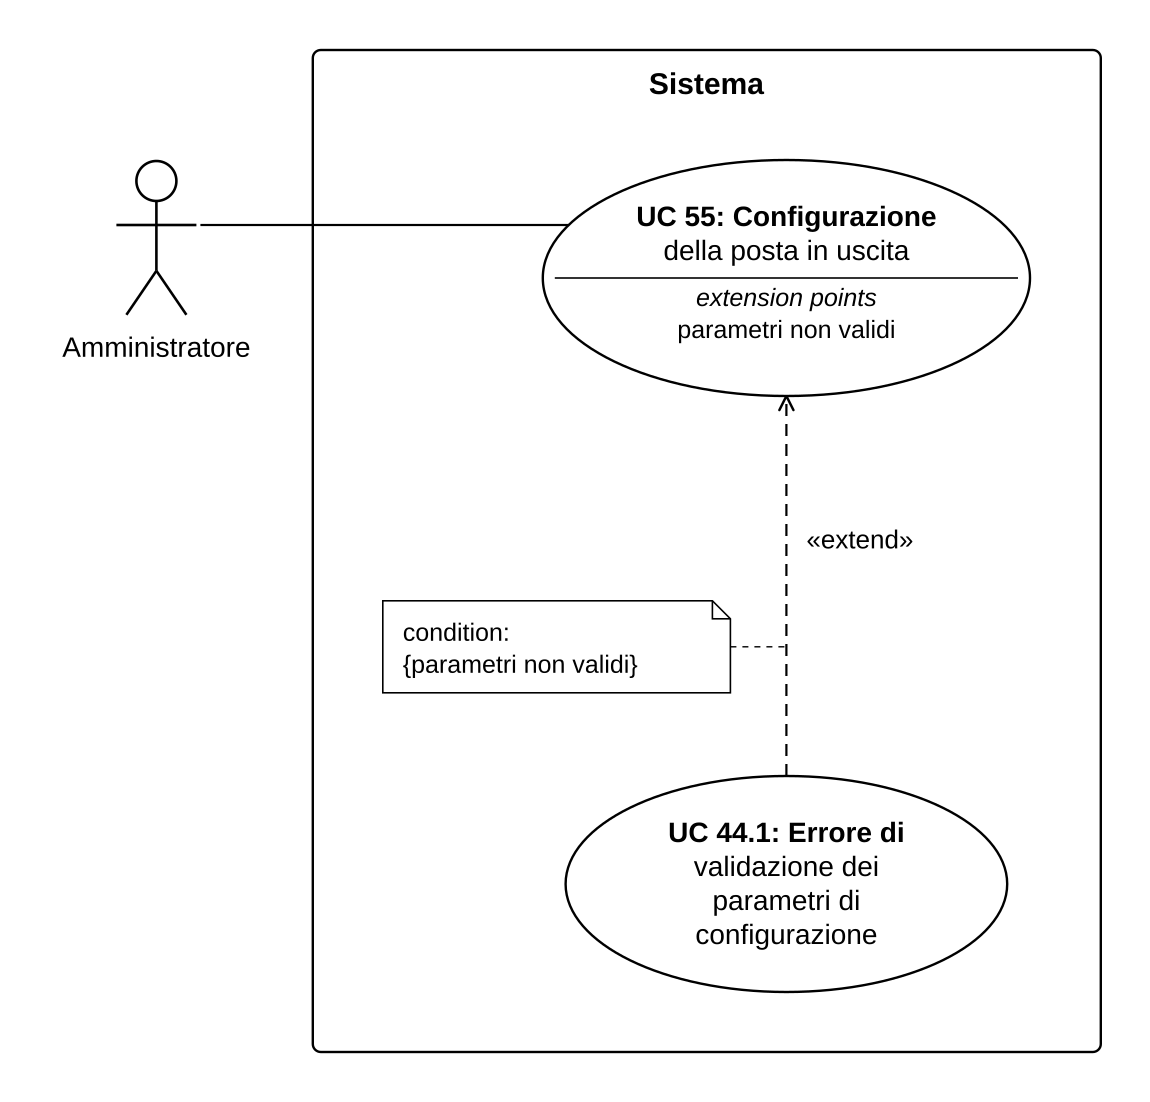
\includegraphics[width=\linewidth,height=0.32\textheight,keepaspectratio]{img/UC55.png}
\caption{UC 55 -- Configurazione della posta in uscita}
\end{center}
\begin{itemize}
    \item \textbf{Attore principale}: Amministratore
    \item \textbf{Precondizioni}: L'Amministratore è autenticato.
    \item \textbf{Scenario principale}:
    \begin{enumerate}
        \item L'Amministratore seleziona la configurazione della posta in uscita.
        \item L'Amministratore inserisce i parametri del servizio.
        \item Il sistema valida i parametri e salva la configurazione.
    \end{enumerate}
    \item \textbf{Postcondizioni}: La posta in uscita è configurata.
    \item \textbf{Trigger}: L'Amministratore vuole configurare la posta in uscita.
    \item \textbf{Estensioni}:
    \begin{itemize}
        \item \hyperref[uc:44.1]{UC 44.1}: Errore di validazione dei parametri di configurazione $\rightarrow$ Condizione: Parametri non validi.
    \end{itemize}
\end{itemize}

\subsubsection{UC 56: Impostazione della soglia di confidenza}\label{uc:56}
\begin{center}
\captionsetup{type=figure}
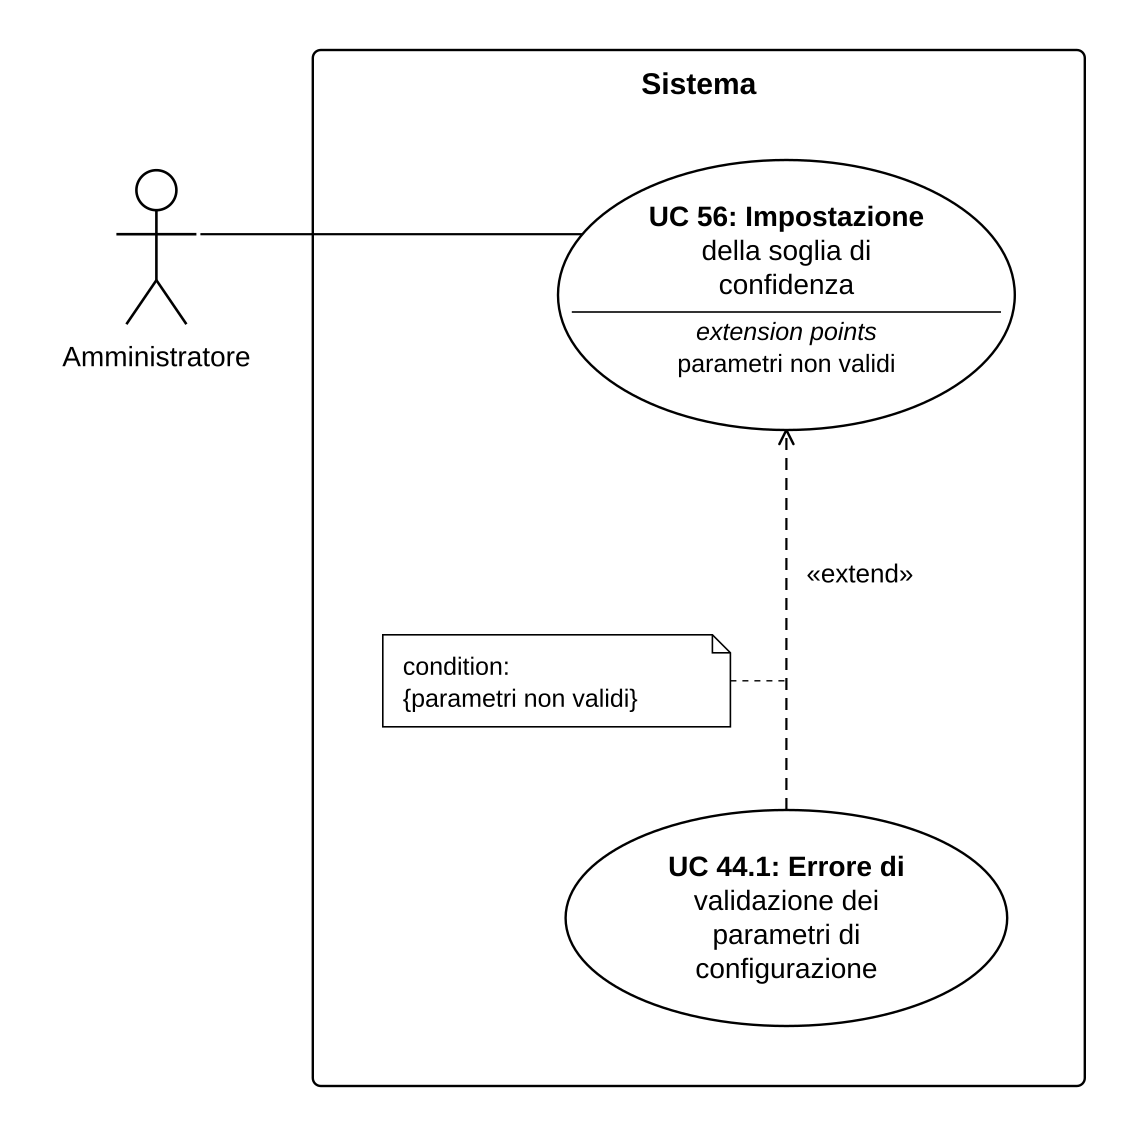
\includegraphics[width=\linewidth,height=0.32\textheight,keepaspectratio]{img/UC56.png}
\caption{UC 56 -- Impostazione della soglia di confidenza}
\end{center}
\begin{itemize}
    \item \textbf{Attore principale}: Amministratore
    \item \textbf{Precondizioni}: L'Amministratore è autenticato.
    \item \textbf{Scenario principale}:
    \begin{enumerate}
        \item L'Amministratore seleziona l'impostazione della soglia di confidenza.
        \item L'Amministratore inserisce il nuovo valore.
        \item Il sistema valida il valore e lo salva.
    \end{enumerate}
    \item \textbf{Postcondizioni}: La soglia di confidenza è aggiornata.
    \item \textbf{Trigger}: L'Amministratore vuole modificare la soglia di confidenza.
    \item \textbf{Estensioni}:
    \begin{itemize}
        \item \hyperref[uc:44.1]{UC 44.1}: Errore di validazione dei parametri di configurazione $\rightarrow$ Condizione: Parametri non validi.
    \end{itemize}
\end{itemize}

\subsubsection{UC 57: Consultazione dello storico dei log}\label{uc:57}
\begin{center}
\captionsetup{type=figure}
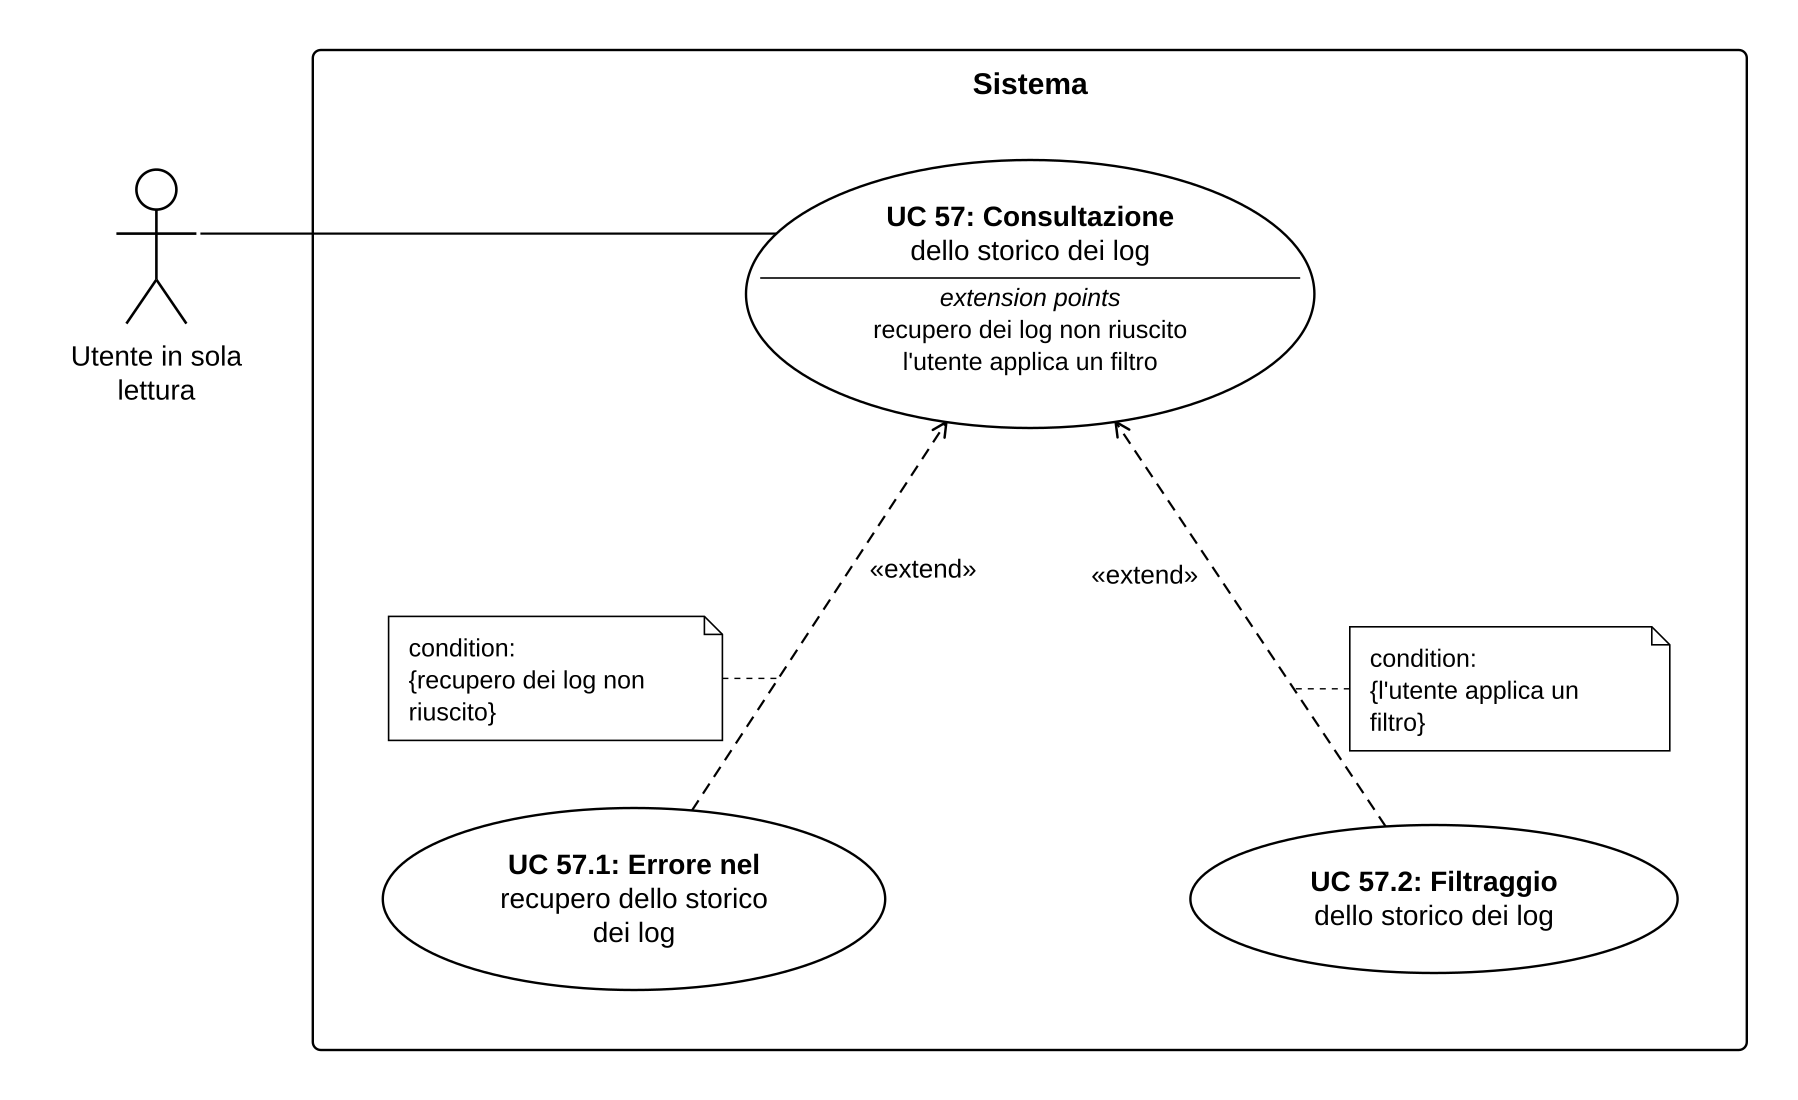
\includegraphics[width=\linewidth,height=0.32\textheight,keepaspectratio]{img/UC57.png}
\caption{UC 57 -- Consultazione dello storico dei log}
\end{center}
\begin{itemize}
    \item \textbf{Attore principale}: Utente in sola lettura
    \item \textbf{Precondizioni}: L'utente è autenticato.
    \item \textbf{Scenario principale}:
    \begin{enumerate}
        \item L'utente apre la dashboard di monitoraggio.
        \item Il sistema recupera lo storico dei log.
        \item Il sistema mostra lo storico.
    \end{enumerate}
    \item \textbf{Postcondizioni}: Lo storico dei log è visualizzato.
    \item \textbf{Trigger}: L'utente vuole consultare i log.
    \item \textbf{Estensioni}:
    \begin{itemize}
        \item \hyperref[uc:57.1]{UC 57.1}: Errore nel recupero dello storico dei log $\rightarrow$ Condizione: Recupero dei log non riuscito.
        \item \hyperref[uc:57.2]{UC 57.2}: Filtraggio dello storico dei log $\rightarrow$ Condizione: L'utente applica un filtro.
    \end{itemize}
\end{itemize}

\subsubsection{UC 57.1: Errore nel recupero dello storico dei log}\label{uc:57.1}
\begin{center}
\captionsetup{type=figure}
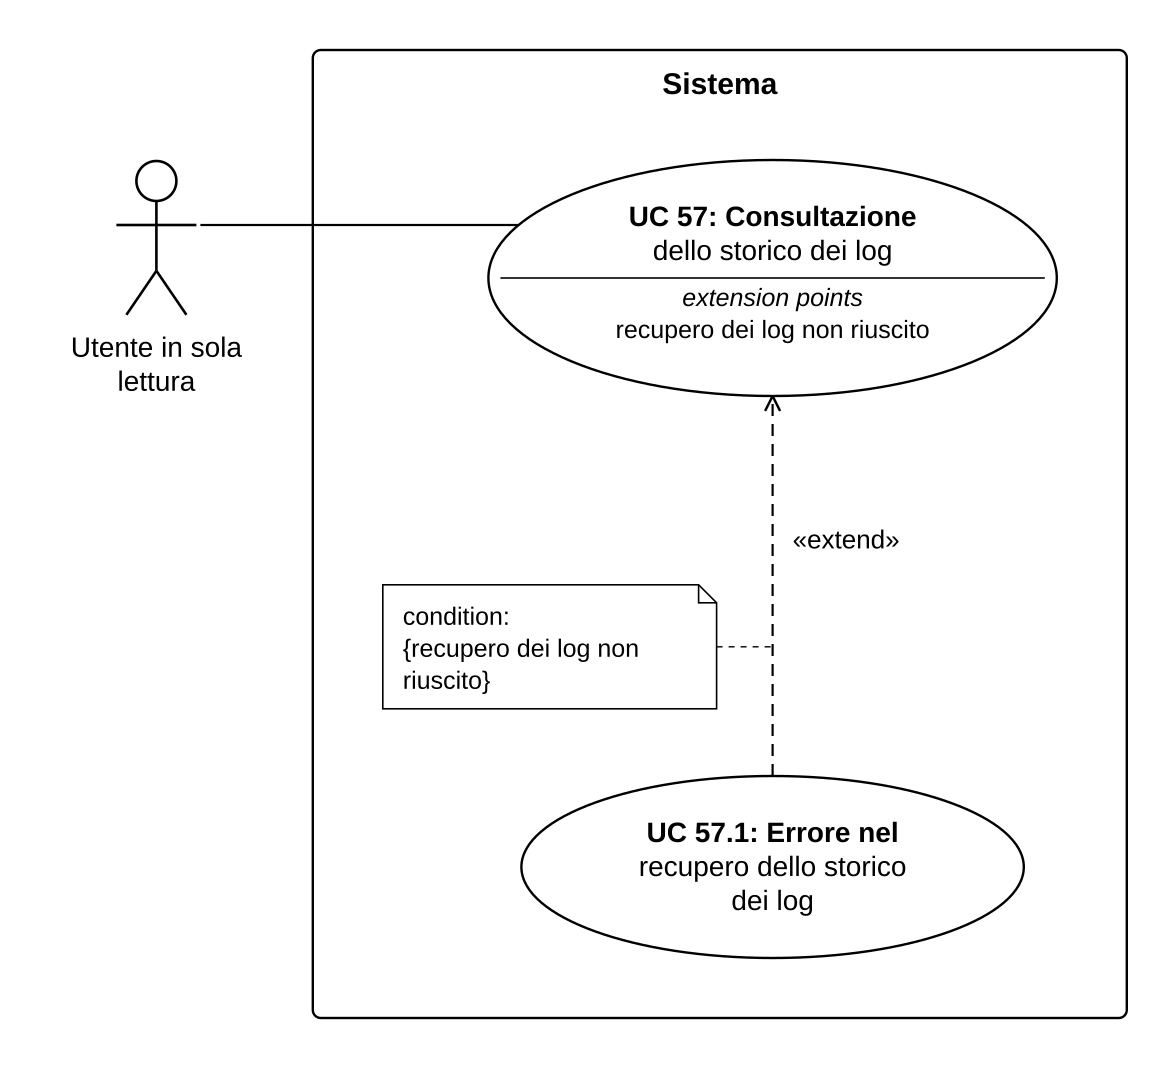
\includegraphics[width=\linewidth,height=0.32\textheight,keepaspectratio]{img/UC57_1.png}
\caption{UC 57.1 -- Errore nel recupero dello storico dei log}
\end{center}
\begin{itemize}
    \item \textbf{Attore principale}: Utente in sola lettura
    \item \textbf{Precondizioni}: Il recupero dello storico dei log è in corso.
    \item \textbf{Scenario principale}:
    \begin{enumerate}
        \item Il sistema rileva un errore nel recupero.
        \item Il sistema segnala l'errore all'utente.
    \end{enumerate}
    \item \textbf{Postcondizioni}: Lo storico non è visualizzato.
    \item \textbf{Trigger}: Recupero dei log non riuscito.
    \item \textbf{Estende}: \hyperref[uc:57]{UC 57}.
\end{itemize}

\subsubsection{UC 57.2: Filtraggio dello storico dei log}\label{uc:57.2}
\begin{center}
\captionsetup{type=figure}
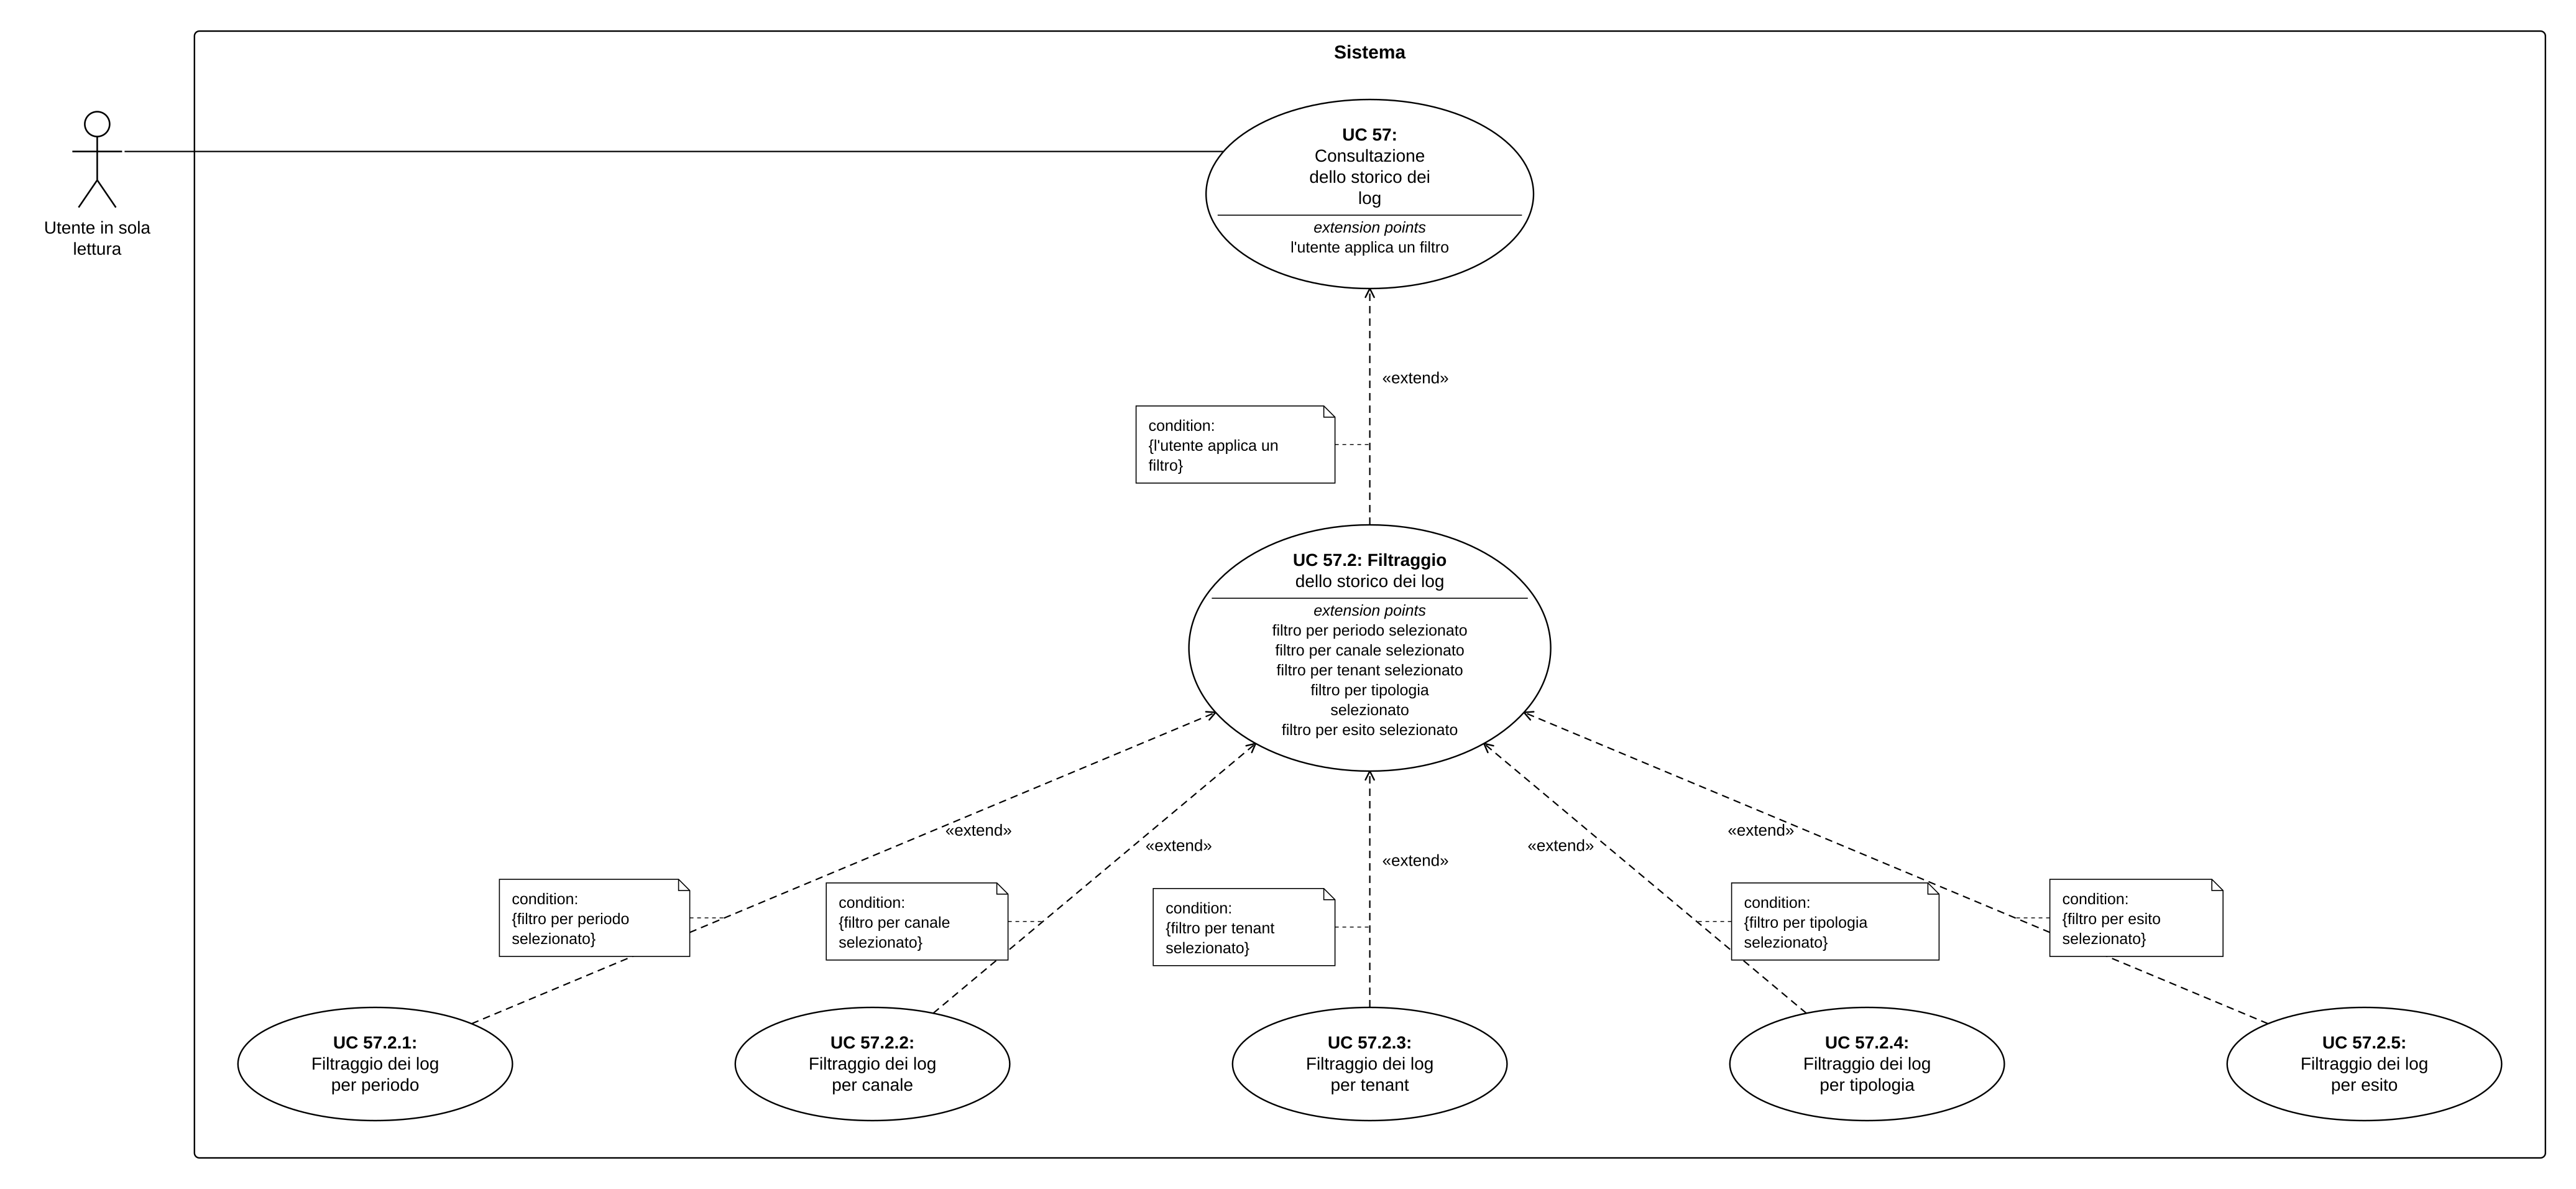
\includegraphics[width=\linewidth,height=0.32\textheight,keepaspectratio]{img/UC57_2.png}
\caption{UC 57.2 -- Filtraggio dello storico dei log}
\end{center}
\begin{itemize}
    \item \textbf{Attore principale}: Utente in sola lettura
    \item \textbf{Precondizioni}: Lo storico dei log è visualizzato.
    \item \textbf{Scenario principale}:
    \begin{enumerate}
        \item L'utente sceglie di filtrare lo storico.
        \item L'utente seleziona uno o più criteri.
        \item Il sistema mostra i log corrispondenti.
    \end{enumerate}
    \item \textbf{Postcondizioni}: Sono visualizzati solo i log che soddisfano i filtri.
    \item \textbf{Trigger}: L'utente vuole restringere lo storico dei log.
    \item \textbf{Estende}: \hyperref[uc:57]{UC 57}.
    \item \textbf{Estensioni}:
    \begin{itemize}
        \item \hyperref[uc:57.2.1]{UC 57.2.1}: Filtraggio dei log per periodo $\rightarrow$ Condizione: Filtro per periodo selezionato.
        \item \hyperref[uc:57.2.2]{UC 57.2.2}: Filtraggio dei log per canale $\rightarrow$ Condizione: Filtro per canale selezionato.
        \item \hyperref[uc:57.2.3]{UC 57.2.3}: Filtraggio dei log per tenant $\rightarrow$ Condizione: Filtro per tenant selezionato.
        \item \hyperref[uc:57.2.4]{UC 57.2.4}: Filtraggio dei log per tipologia $\rightarrow$ Condizione: Filtro per tipologia selezionato.
        \item \hyperref[uc:57.2.5]{UC 57.2.5}: Filtraggio dei log per esito $\rightarrow$ Condizione: Filtro per esito selezionato.
    \end{itemize}
\end{itemize}

\subsubsection{UC 57.2.1: Filtraggio dei log per periodo}\label{uc:57.2.1}
\begin{center}
\captionsetup{type=figure}
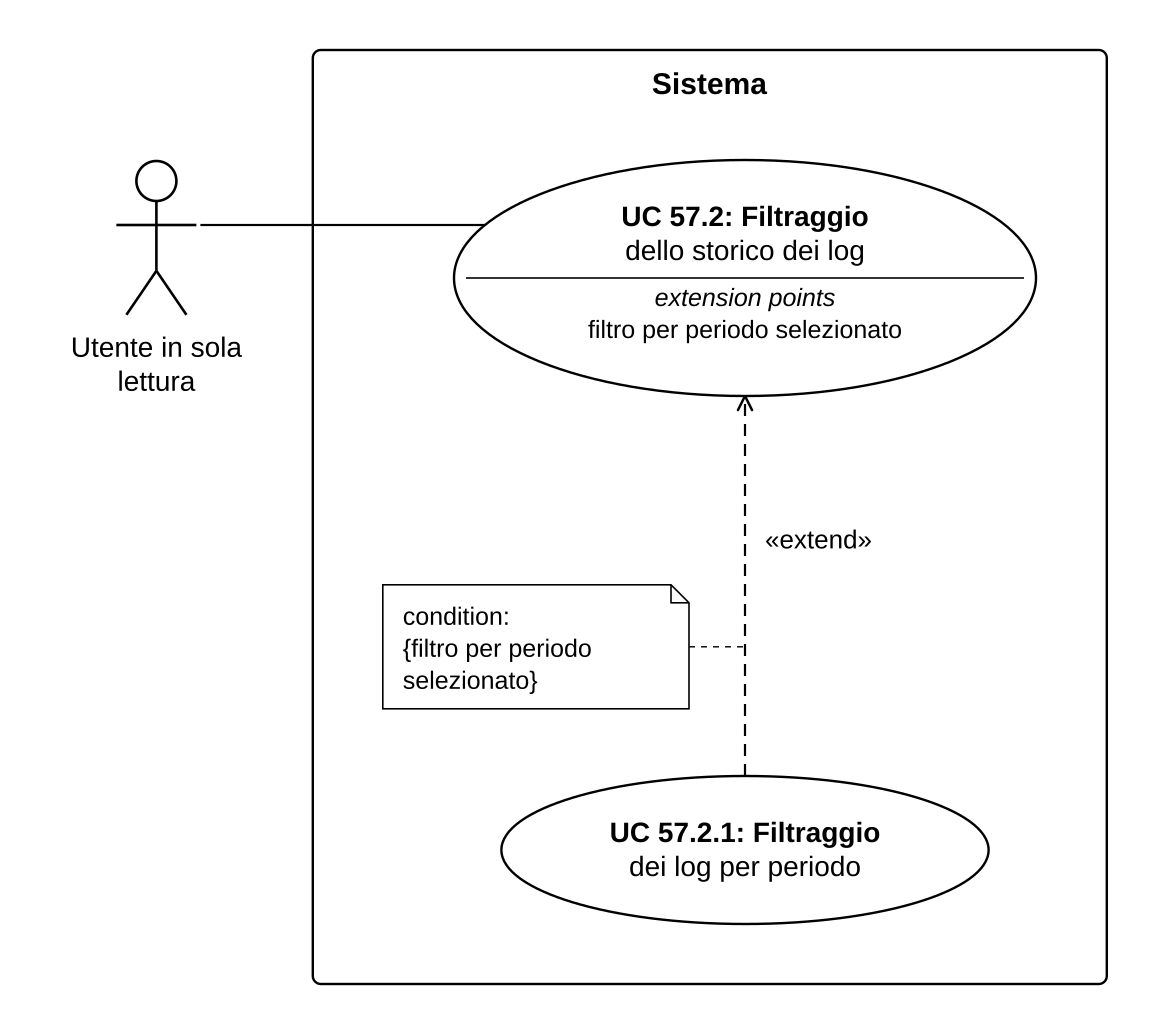
\includegraphics[width=\linewidth,height=0.32\textheight,keepaspectratio]{img/UC57_2_1.png}
\caption{UC 57.2.1 -- Filtraggio dei log per periodo}
\end{center}
\begin{itemize}
    \item \textbf{Attore principale}: Utente in sola lettura
    \item \textbf{Precondizioni}: Il filtraggio dei log è attivo.
    \item \textbf{Scenario principale}:
    \begin{enumerate}
        \item L'utente indica un intervallo di date.
        \item Il sistema mostra i log del periodo.
    \end{enumerate}
    \item \textbf{Postcondizioni}: Sono visualizzati i log del periodo indicato.
    \item \textbf{Trigger}: L'utente vuole filtrare per periodo.
    \item \textbf{Estende}: \hyperref[uc:57.2]{UC 57.2}.
\end{itemize}

\subsubsection{UC 57.2.2: Filtraggio dei log per canale}\label{uc:57.2.2}
\begin{center}
\captionsetup{type=figure}
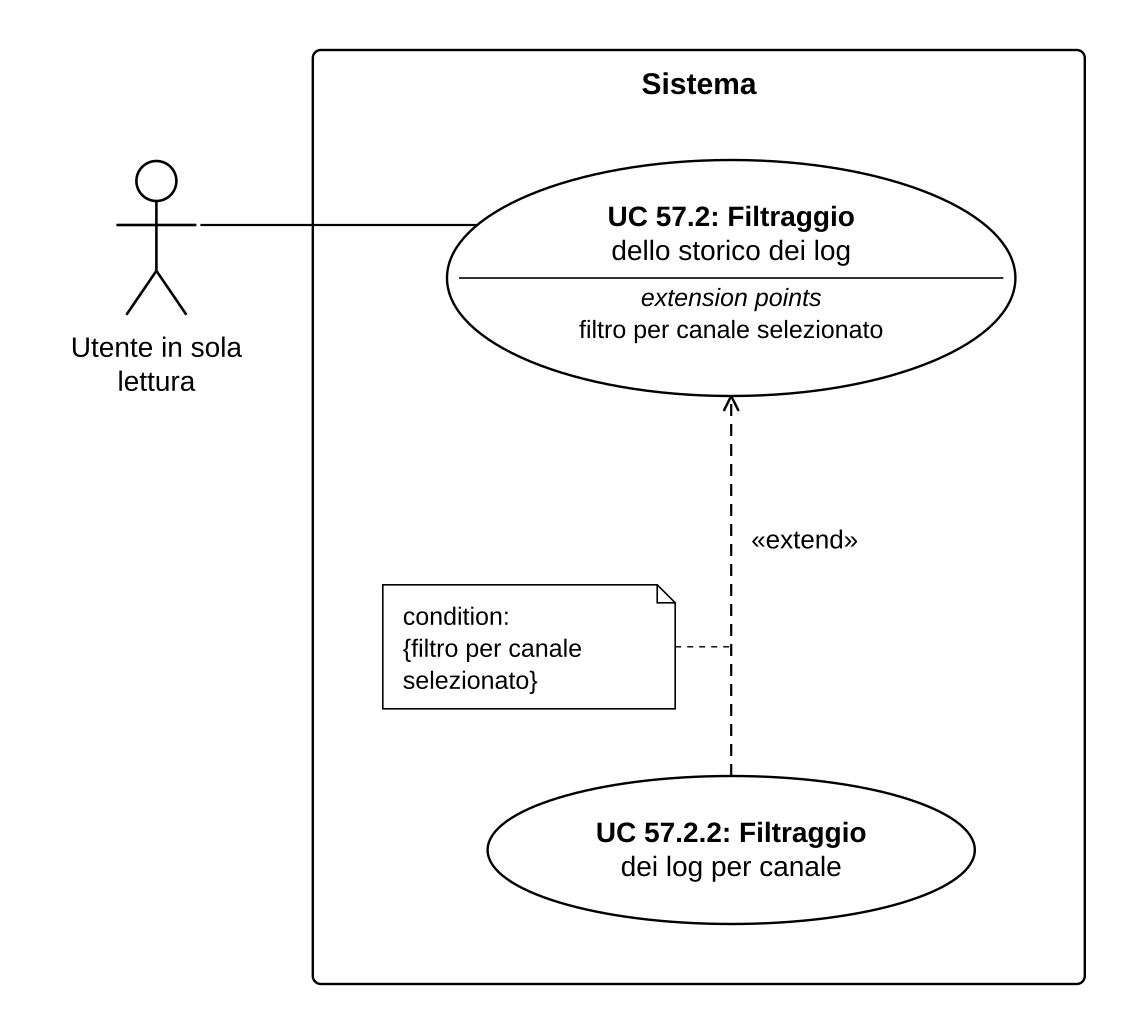
\includegraphics[width=\linewidth,height=0.32\textheight,keepaspectratio]{img/UC57_2_2.png}
\caption{UC 57.2.2 -- Filtraggio dei log per canale}
\end{center}
\begin{itemize}
    \item \textbf{Attore principale}: Utente in sola lettura
    \item \textbf{Precondizioni}: Il filtraggio dei log è attivo.
    \item \textbf{Scenario principale}:
    \begin{enumerate}
        \item L'utente seleziona un canale.
        \item Il sistema mostra i log relativi al canale.
    \end{enumerate}
    \item \textbf{Postcondizioni}: Sono visualizzati i log del canale scelto.
    \item \textbf{Trigger}: L'utente vuole filtrare per canale.
    \item \textbf{Estende}: \hyperref[uc:57.2]{UC 57.2}.
\end{itemize}

\subsubsection{UC 57.2.3: Filtraggio dei log per tenant}\label{uc:57.2.3}
\begin{center}
\captionsetup{type=figure}
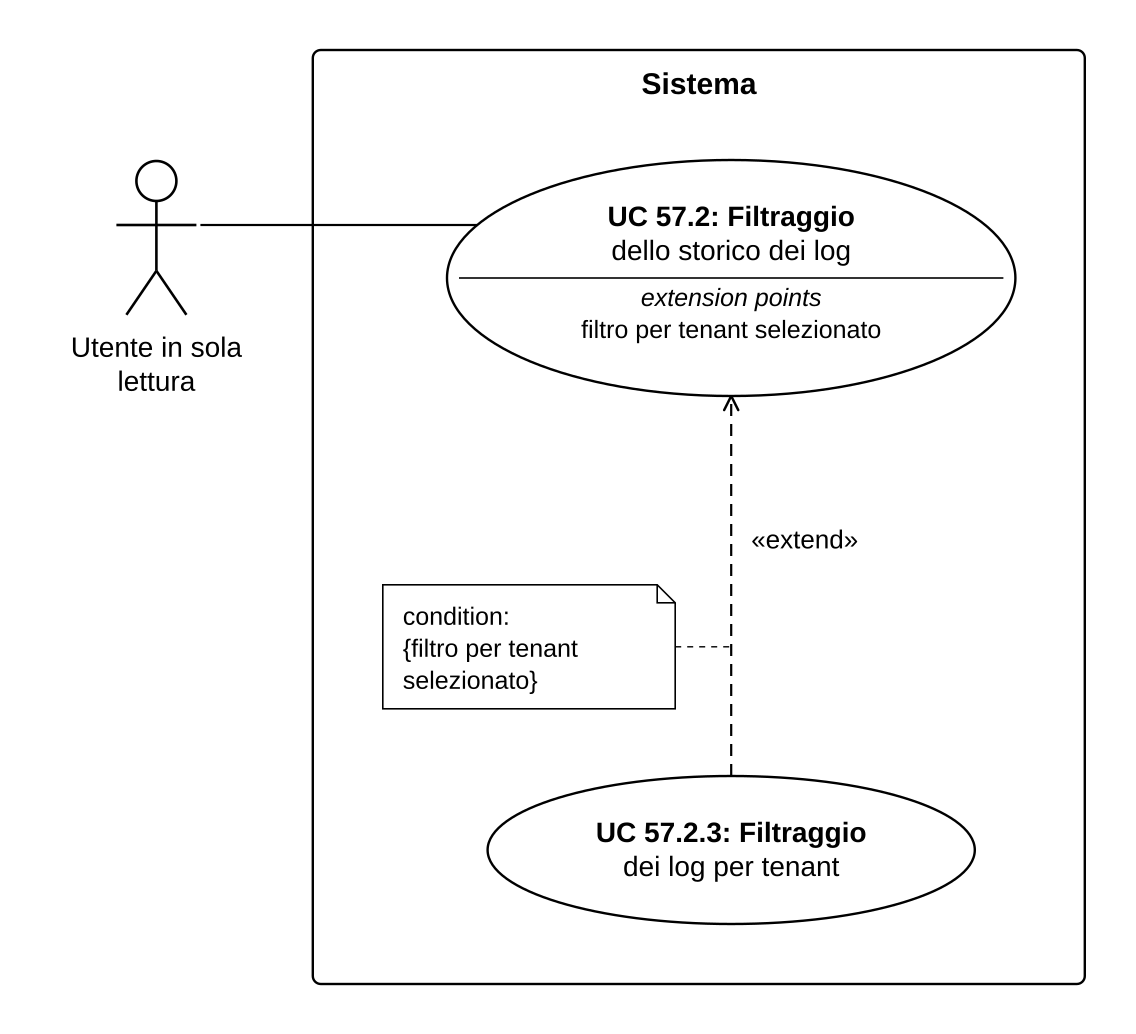
\includegraphics[width=\linewidth,height=0.32\textheight,keepaspectratio]{img/UC57_2_3.png}
\caption{UC 57.2.3 -- Filtraggio dei log per tenant}
\end{center}
\begin{itemize}
    \item \textbf{Attore principale}: Utente in sola lettura
    \item \textbf{Precondizioni}: Il filtraggio dei log è attivo.
    \item \textbf{Scenario principale}:
    \begin{enumerate}
        \item L'utente seleziona un tenant.
        \item Il sistema mostra i log relativi al tenant.
    \end{enumerate}
    \item \textbf{Postcondizioni}: Sono visualizzati i log del tenant scelto.
    \item \textbf{Trigger}: L'utente vuole filtrare per tenant.
    \item \textbf{Estende}: \hyperref[uc:57.2]{UC 57.2}.
\end{itemize}

\subsubsection{UC 57.2.4: Filtraggio dei log per tipologia}\label{uc:57.2.4}
\begin{center}
\captionsetup{type=figure}
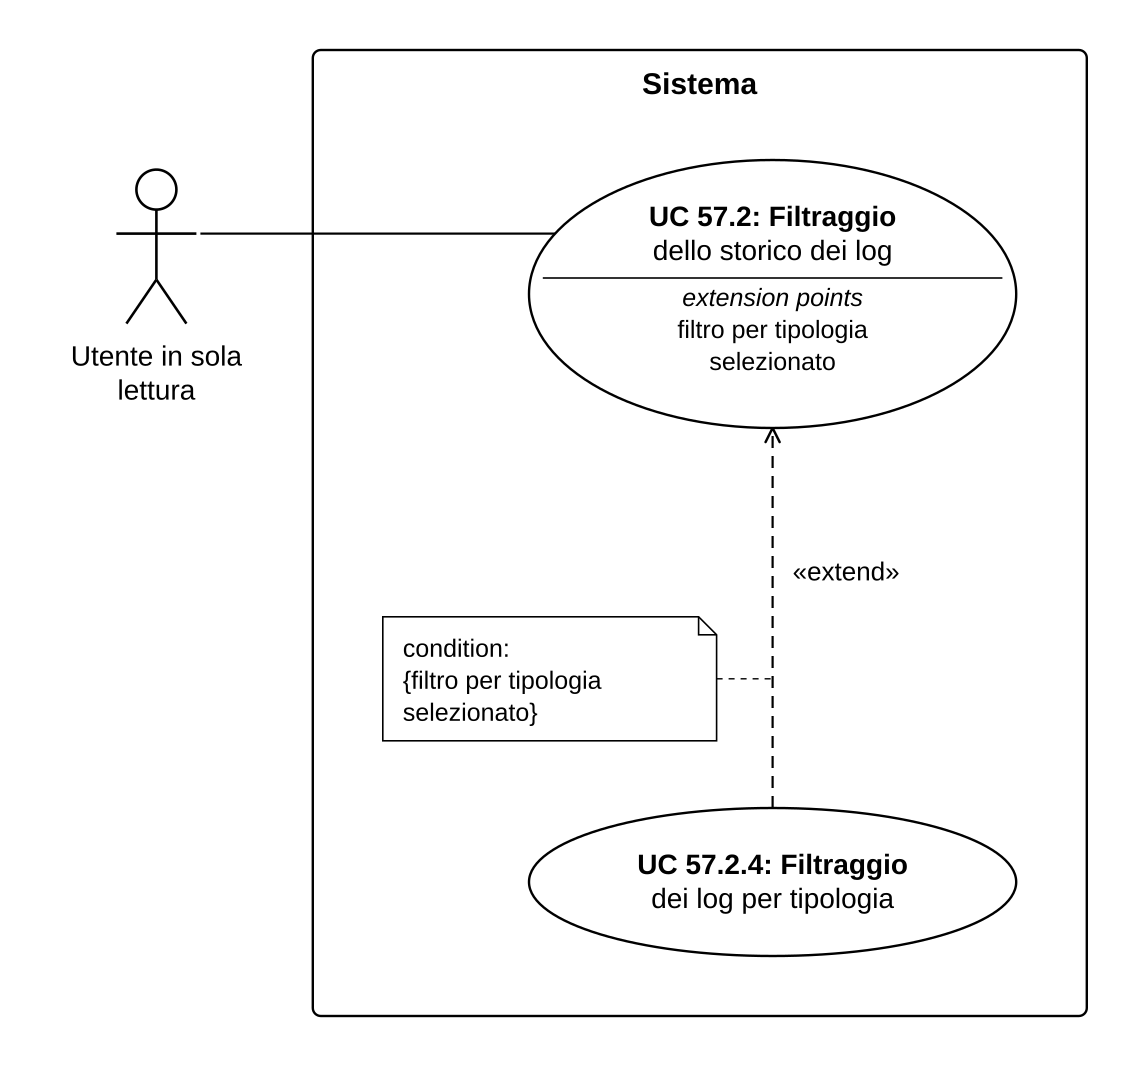
\includegraphics[width=\linewidth,height=0.32\textheight,keepaspectratio]{img/UC57_2_4.png}
\caption{UC 57.2.4 -- Filtraggio dei log per tipologia}
\end{center}
\begin{itemize}
    \item \textbf{Attore principale}: Utente in sola lettura
    \item \textbf{Precondizioni}: Il filtraggio dei log è attivo.
    \item \textbf{Scenario principale}:
    \begin{enumerate}
        \item L'utente seleziona una tipologia di richiesta.
        \item Il sistema mostra i log relativi alla tipologia.
    \end{enumerate}
    \item \textbf{Postcondizioni}: Sono visualizzati i log della tipologia scelta.
    \item \textbf{Trigger}: L'utente vuole filtrare per tipologia.
    \item \textbf{Estende}: \hyperref[uc:57.2]{UC 57.2}.
\end{itemize}

\subsubsection{UC 57.2.5: Filtraggio dei log per esito}\label{uc:57.2.5}
\begin{center}
\captionsetup{type=figure}
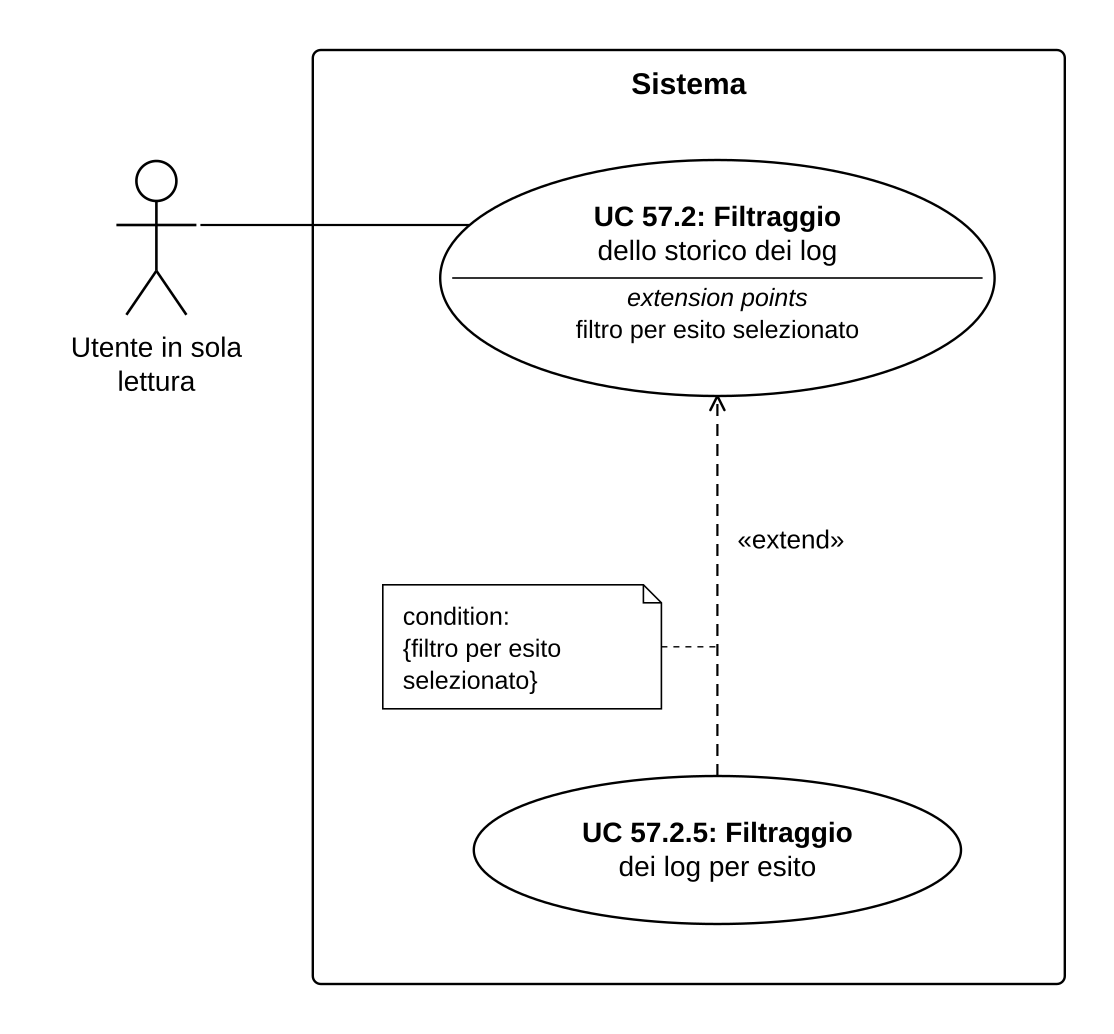
\includegraphics[width=\linewidth,height=0.32\textheight,keepaspectratio]{img/UC57_2_5.png}
\caption{UC 57.2.5 -- Filtraggio dei log per esito}
\end{center}
\begin{itemize}
    \item \textbf{Attore principale}: Utente in sola lettura
    \item \textbf{Precondizioni}: Il filtraggio dei log è attivo.
    \item \textbf{Scenario principale}:
    \begin{enumerate}
        \item L'utente seleziona un esito.
        \item Il sistema mostra i log con tale esito.
    \end{enumerate}
    \item \textbf{Postcondizioni}: Sono visualizzati i log con l'esito scelto.
    \item \textbf{Trigger}: L'utente vuole filtrare per esito.
    \item \textbf{Estende}: \hyperref[uc:57.2]{UC 57.2}.
\end{itemize}

\subsubsection{UC 58: Consultazione delle richieste persistite e del loro stato}\label{uc:58}
\begin{center}
\captionsetup{type=figure}
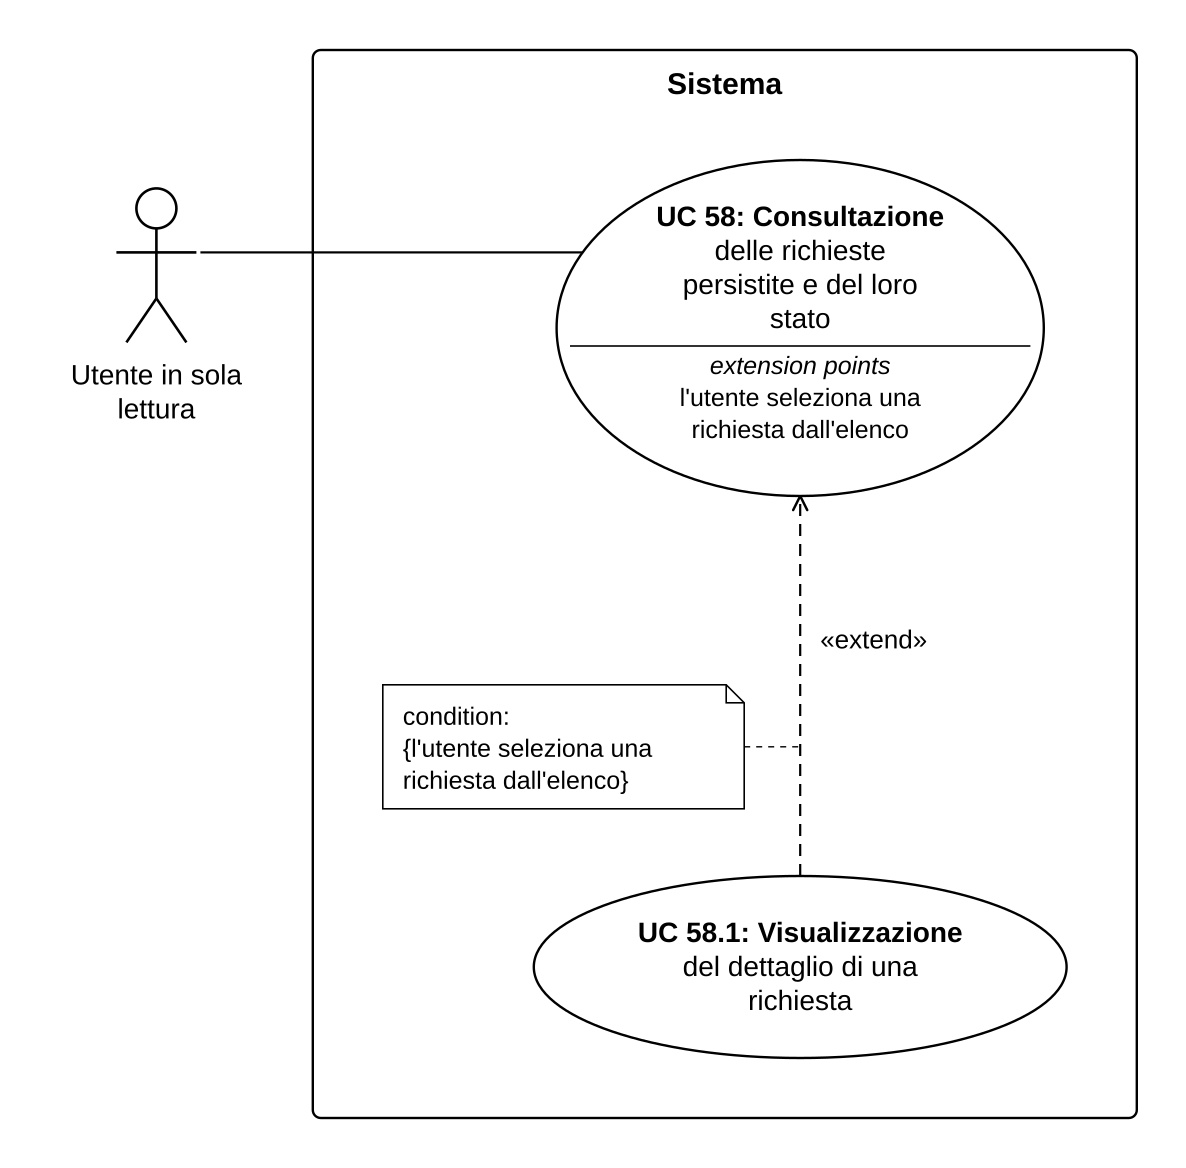
\includegraphics[width=\linewidth,height=0.32\textheight,keepaspectratio]{img/UC58.png}
\caption{UC 58 -- Consultazione delle richieste persistite e del loro stato}
\end{center}
\begin{itemize}
    \item \textbf{Attore principale}: Utente in sola lettura
    \item \textbf{Precondizioni}: L'utente è autenticato.
    \item \textbf{Scenario principale}:
    \begin{enumerate}
        \item L'utente apre la sezione delle richieste.
        \item Il sistema mostra le richieste persistite con il loro stato, incluse quelle non riuscite.
    \end{enumerate}
    \item \textbf{Postcondizioni}: L'elenco delle richieste è visualizzato.
    \item \textbf{Trigger}: L'utente vuole consultare le richieste.
    \item \textbf{Estensioni}:
    \begin{itemize}
        \item \hyperref[uc:58.1]{UC 58.1}: Visualizzazione del dettaglio di una richiesta $\rightarrow$ Condizione: L'utente seleziona una richiesta dall'elenco.
    \end{itemize}
\end{itemize}

\subsubsection{UC 58.1: Visualizzazione del dettaglio di una richiesta}\label{uc:58.1}
\begin{center}
\captionsetup{type=figure}
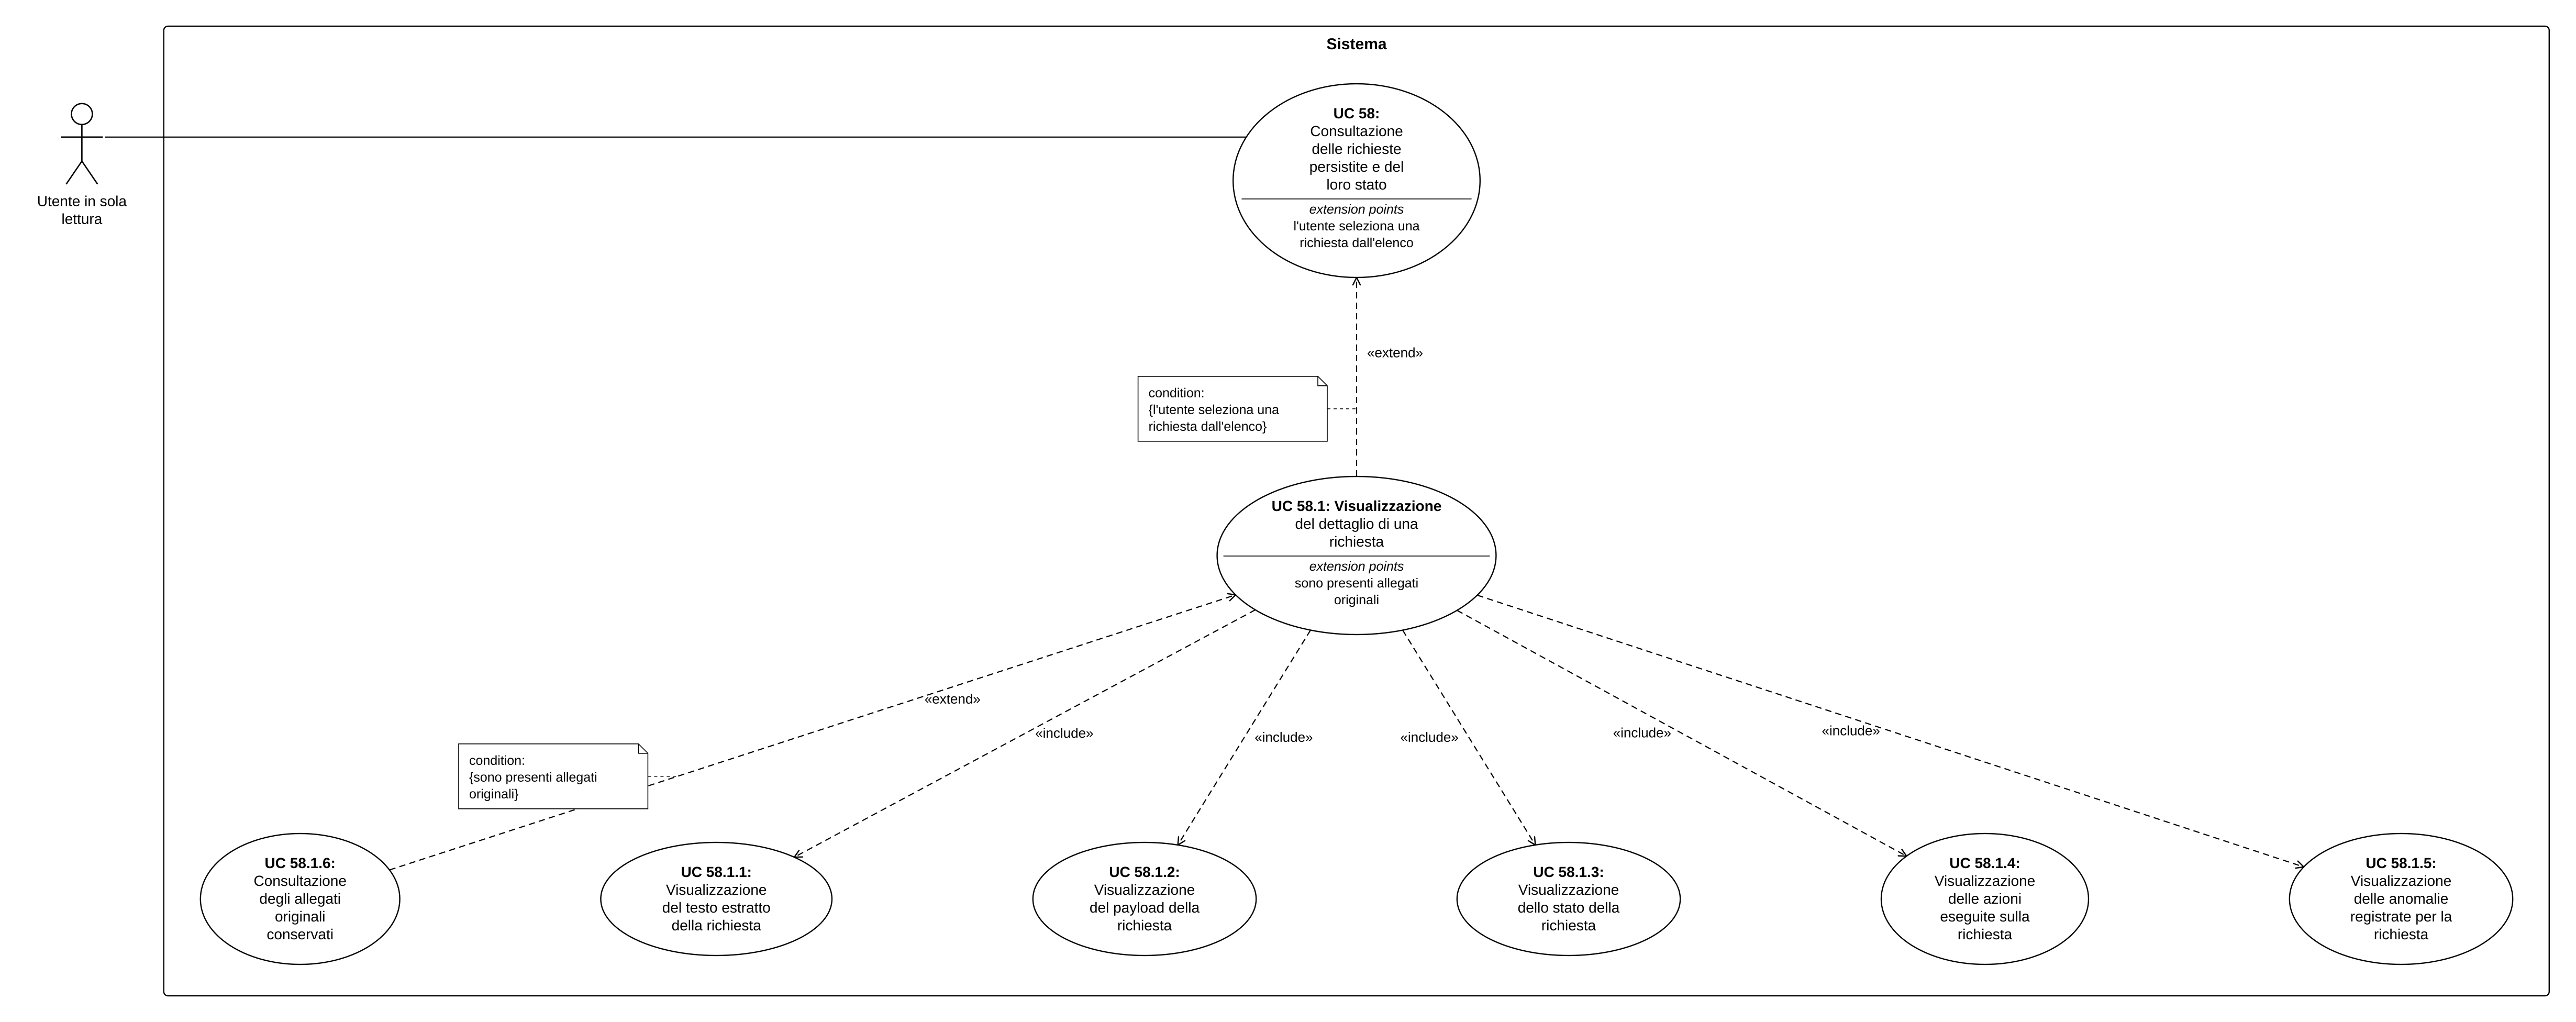
\includegraphics[width=\linewidth,height=0.32\textheight,keepaspectratio]{img/UC58_1.png}
\caption{UC 58.1 -- Visualizzazione del dettaglio di una richiesta}
\end{center}
\begin{itemize}
    \item \textbf{Attore principale}: Utente in sola lettura
    \item \textbf{Precondizioni}: L'elenco delle richieste è visualizzato.
    \item \textbf{Scenario principale}:
    \begin{enumerate}
        \item L'utente seleziona una richiesta.
        \item Il sistema mostra testo estratto, payload, stato, azioni eseguite e anomalie.
    \end{enumerate}
    \item \textbf{Postcondizioni}: Il dettaglio della richiesta è visualizzato.
    \item \textbf{Trigger}: L'utente vuole approfondire una richiesta.
    \item \textbf{Estende}: \hyperref[uc:58]{UC 58}.
    \item \textbf{Inclusioni}:
    \begin{itemize}
        \item \hyperref[uc:58.1.1]{UC 58.1.1}: Visualizzazione del testo estratto della richiesta
        \item \hyperref[uc:58.1.2]{UC 58.1.2}: Visualizzazione del payload della richiesta
        \item \hyperref[uc:58.1.3]{UC 58.1.3}: Visualizzazione dello stato della richiesta
        \item \hyperref[uc:58.1.4]{UC 58.1.4}: Visualizzazione delle azioni eseguite sulla richiesta
        \item \hyperref[uc:58.1.5]{UC 58.1.5}: Visualizzazione delle anomalie registrate per la richiesta
    \end{itemize}
    \item \textbf{Estensioni}:
    \begin{itemize}
        \item \hyperref[uc:58.1.6]{UC 58.1.6}: Consultazione degli allegati originali conservati $\rightarrow$ Condizione: Sono presenti allegati originali.
    \end{itemize}
\end{itemize}

\subsubsection{UC 58.1.1: Visualizzazione del testo estratto della richiesta}\label{uc:58.1.1}
\begin{center}
\captionsetup{type=figure}
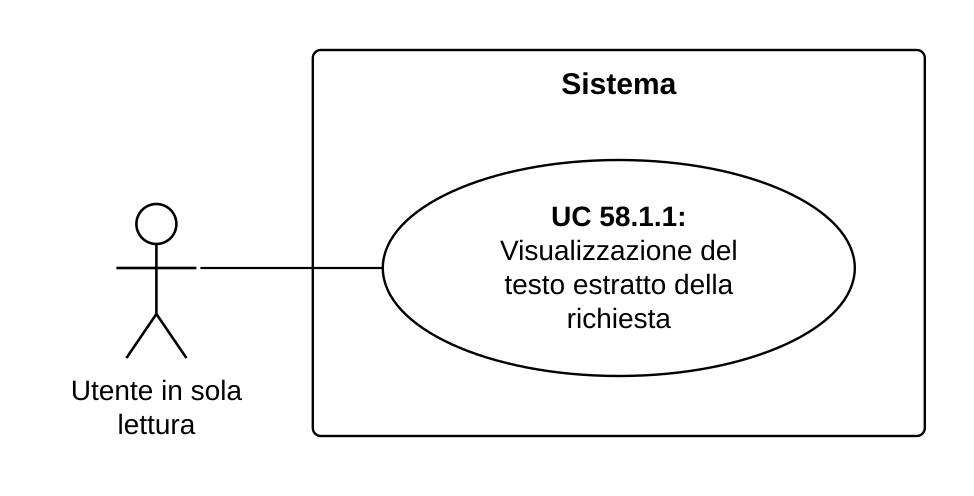
\includegraphics[width=\linewidth,height=0.32\textheight,keepaspectratio]{img/UC58_1_1.png}
\caption{UC 58.1.1 -- Visualizzazione del testo estratto della richiesta}
\end{center}
\begin{itemize}
    \item \textbf{Attore principale}: Utente in sola lettura
    \item \textbf{Precondizioni}: Il dettaglio di una richiesta è in visualizzazione.
    \item \textbf{Scenario principale}:
    \begin{enumerate}
        \item Il sistema mostra il testo estratto dalla richiesta.
    \end{enumerate}
    \item \textbf{Postcondizioni}: Il testo estratto è visualizzato.
    \item \textbf{Trigger}: Apertura del dettaglio della richiesta.
    \item \textbf{Incluso da}: \hyperref[uc:58.1]{UC 58.1}.
\end{itemize}

\subsubsection{UC 58.1.2: Visualizzazione del payload della richiesta}\label{uc:58.1.2}
\begin{center}
\captionsetup{type=figure}
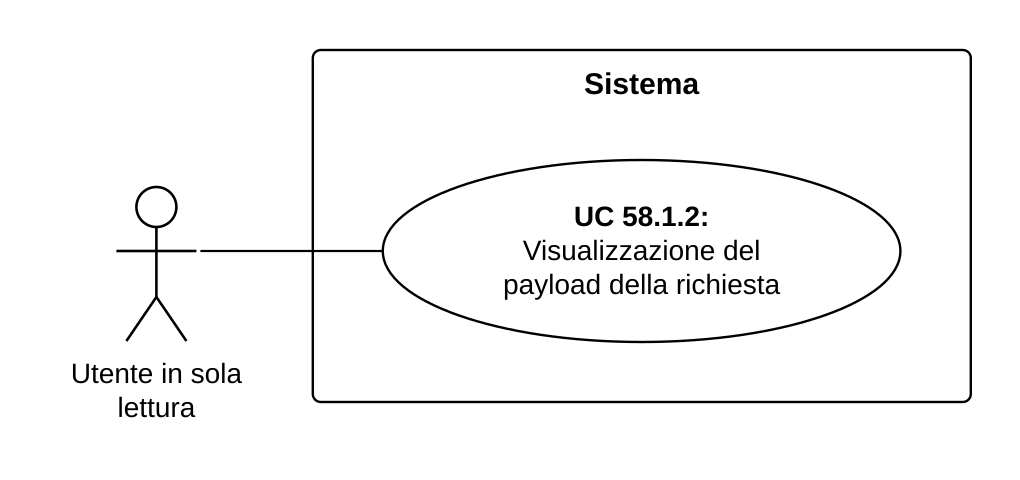
\includegraphics[width=\linewidth,height=0.32\textheight,keepaspectratio]{img/UC58_1_2.png}
\caption{UC 58.1.2 -- Visualizzazione del payload della richiesta}
\end{center}
\begin{itemize}
    \item \textbf{Attore principale}: Utente in sola lettura
    \item \textbf{Precondizioni}: Il dettaglio di una richiesta è in visualizzazione.
    \item \textbf{Scenario principale}:
    \begin{enumerate}
        \item Il sistema mostra il payload JSON della richiesta.
    \end{enumerate}
    \item \textbf{Postcondizioni}: Il payload è visualizzato.
    \item \textbf{Trigger}: Apertura del dettaglio della richiesta.
    \item \textbf{Incluso da}: \hyperref[uc:58.1]{UC 58.1}.
\end{itemize}

\subsubsection{UC 58.1.3: Visualizzazione dello stato della richiesta}\label{uc:58.1.3}
\begin{center}
\captionsetup{type=figure}
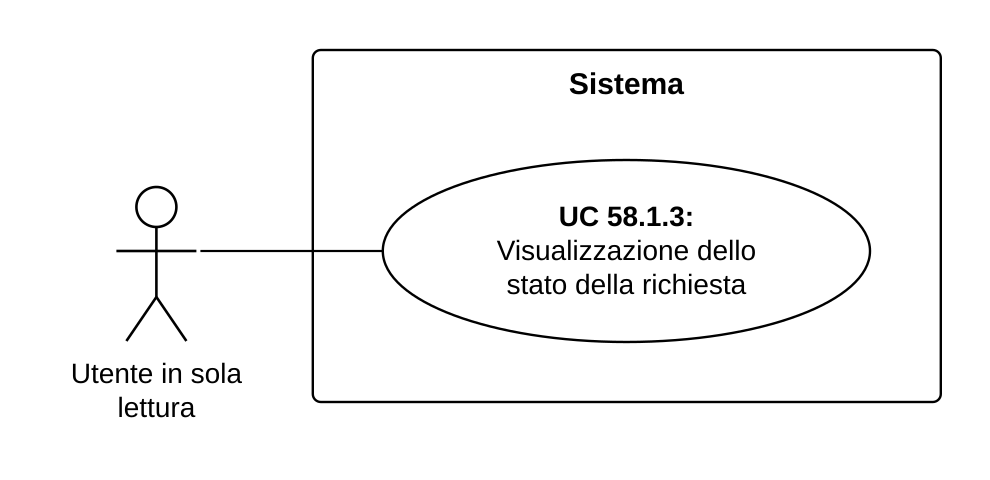
\includegraphics[width=\linewidth,height=0.32\textheight,keepaspectratio]{img/UC58_1_3.png}
\caption{UC 58.1.3 -- Visualizzazione dello stato della richiesta}
\end{center}
\begin{itemize}
    \item \textbf{Attore principale}: Utente in sola lettura
    \item \textbf{Precondizioni}: Il dettaglio di una richiesta è in visualizzazione.
    \item \textbf{Scenario principale}:
    \begin{enumerate}
        \item Il sistema mostra lo stato di avanzamento della richiesta.
    \end{enumerate}
    \item \textbf{Postcondizioni}: Lo stato è visualizzato.
    \item \textbf{Trigger}: Apertura del dettaglio della richiesta.
    \item \textbf{Incluso da}: \hyperref[uc:58.1]{UC 58.1}.
\end{itemize}

\subsubsection{UC 58.1.4: Visualizzazione delle azioni eseguite sulla richiesta}\label{uc:58.1.4}
\begin{center}
\captionsetup{type=figure}
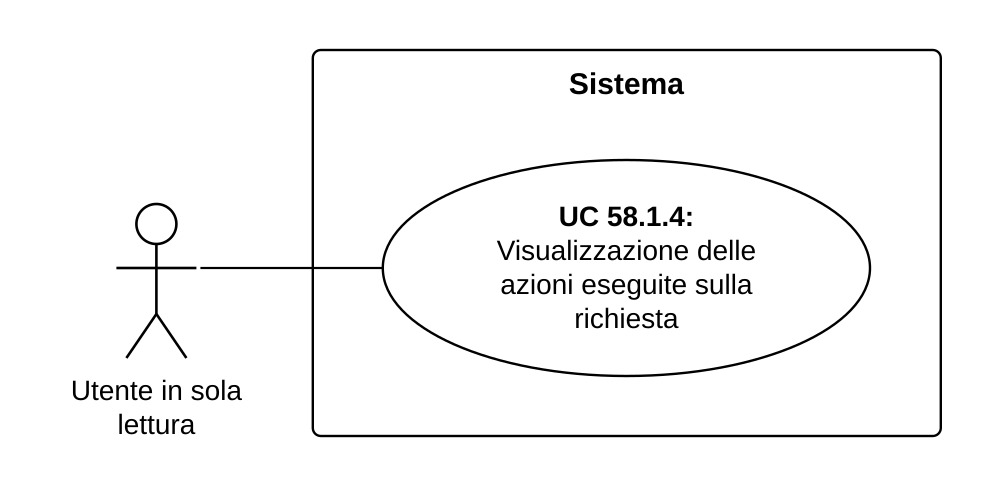
\includegraphics[width=\linewidth,height=0.32\textheight,keepaspectratio]{img/UC58_1_4.png}
\caption{UC 58.1.4 -- Visualizzazione delle azioni eseguite sulla richiesta}
\end{center}
\begin{itemize}
    \item \textbf{Attore principale}: Utente in sola lettura
    \item \textbf{Precondizioni}: Il dettaglio di una richiesta è in visualizzazione.
    \item \textbf{Scenario principale}:
    \begin{enumerate}
        \item Il sistema mostra le azioni eseguite sulla richiesta.
    \end{enumerate}
    \item \textbf{Postcondizioni}: Le azioni eseguite sono visualizzate.
    \item \textbf{Trigger}: Apertura del dettaglio della richiesta.
    \item \textbf{Incluso da}: \hyperref[uc:58.1]{UC 58.1}.
\end{itemize}

\subsubsection{UC 58.1.5: Visualizzazione delle anomalie registrate per la richiesta}\label{uc:58.1.5}
\begin{center}
\captionsetup{type=figure}
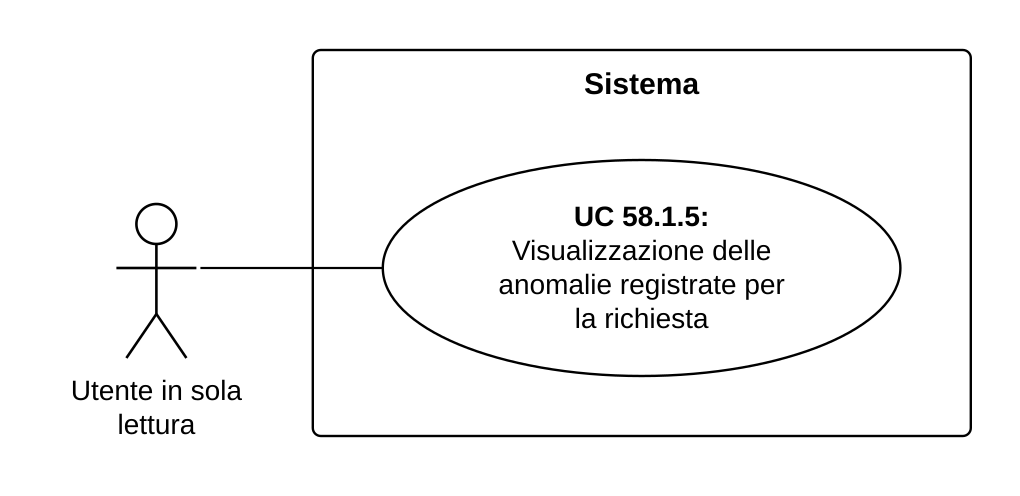
\includegraphics[width=\linewidth,height=0.32\textheight,keepaspectratio]{img/UC58_1_5.png}
\caption{UC 58.1.5 -- Visualizzazione delle anomalie registrate per la richiesta}
\end{center}
\begin{itemize}
    \item \textbf{Attore principale}: Utente in sola lettura
    \item \textbf{Precondizioni}: Il dettaglio di una richiesta è in visualizzazione.
    \item \textbf{Scenario principale}:
    \begin{enumerate}
        \item Il sistema mostra le anomalie registrate per la richiesta.
    \end{enumerate}
    \item \textbf{Postcondizioni}: Le anomalie sono visualizzate.
    \item \textbf{Trigger}: Apertura del dettaglio della richiesta.
    \item \textbf{Incluso da}: \hyperref[uc:58.1]{UC 58.1}.
\end{itemize}

\subsubsection{UC 58.1.6: Consultazione degli allegati originali conservati}\label{uc:58.1.6}
\begin{center}
\captionsetup{type=figure}
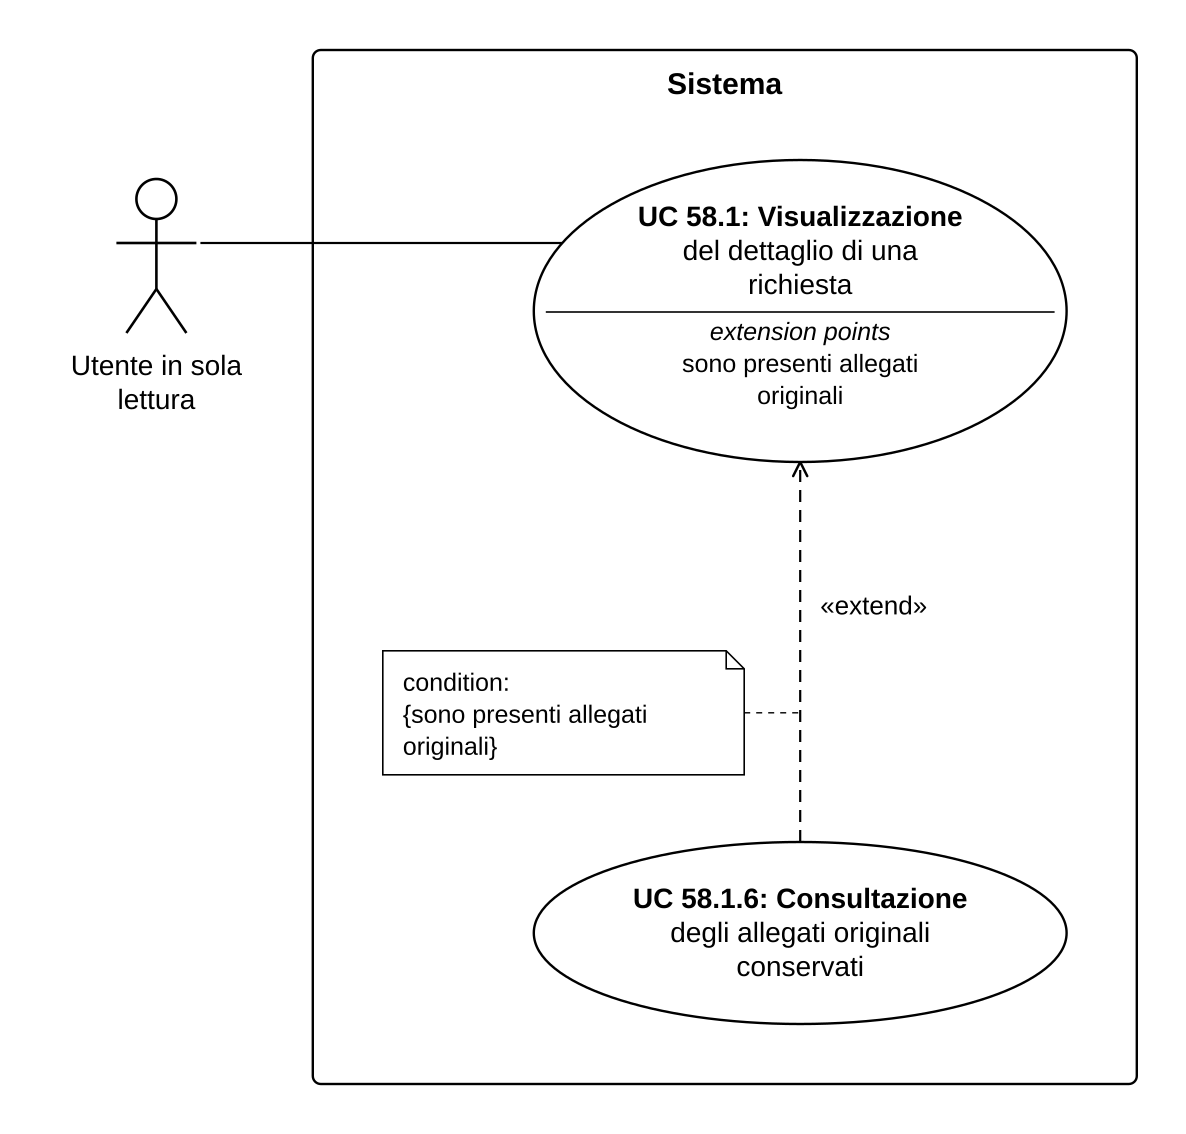
\includegraphics[width=\linewidth,height=0.32\textheight,keepaspectratio]{img/UC58_1_6.png}
\caption{UC 58.1.6 -- Consultazione degli allegati originali conservati}
\end{center}
\begin{itemize}
    \item \textbf{Attore principale}: Utente in sola lettura
    \item \textbf{Precondizioni}: Il dettaglio di una richiesta è in visualizzazione e la richiesta ha allegati originali conservati.
    \item \textbf{Scenario principale}:
    \begin{enumerate}
        \item L'utente seleziona un allegato.
        \item Il sistema decifra e mostra l'allegato originale.
    \end{enumerate}
    \item \textbf{Postcondizioni}: L'allegato originale è consultabile per verifica e debugging.
    \item \textbf{Trigger}: L'utente vuole verificare un allegato originale.
    \item \textbf{Estende}: \hyperref[uc:58.1]{UC 58.1}.
\end{itemize}

\subsubsection{UC 59: Ritentativo dell'inoltro di una richiesta}\label{uc:59}
\begin{center}
\captionsetup{type=figure}
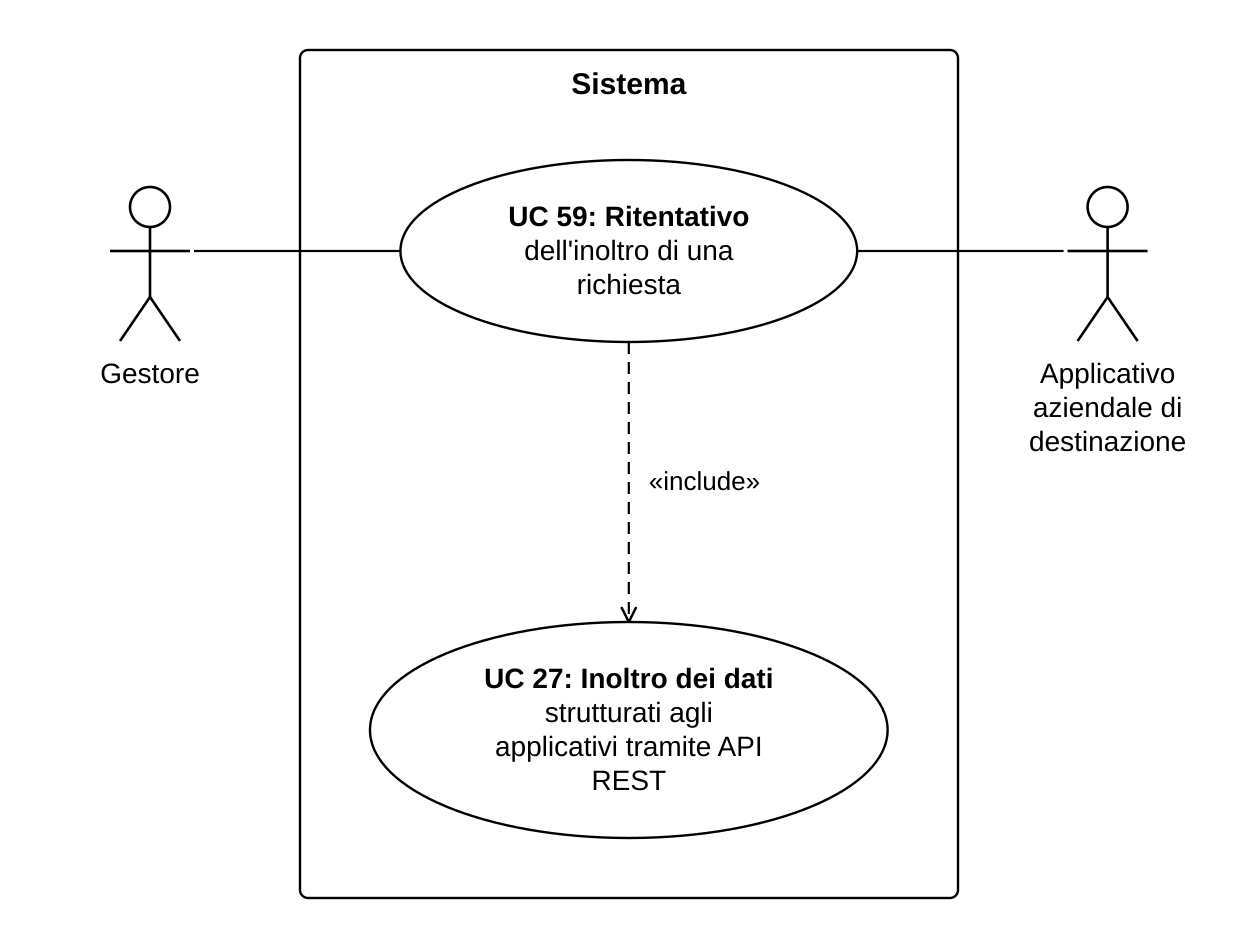
\includegraphics[width=\linewidth,height=0.32\textheight,keepaspectratio]{img/UC59.png}
\caption{UC 59 -- Ritentativo dell'inoltro di una richiesta}
\end{center}
\begin{itemize}
    \item \textbf{Attore principale}: Gestore
    \item \textbf{Attori secondari}: Applicativo aziendale di destinazione
    \item \textbf{Precondizioni}: Il Gestore è autenticato e la richiesta è in stato di inoltro fallito.
    \item \textbf{Scenario principale}:
    \begin{enumerate}
        \item Il Gestore seleziona la richiesta in stato di inoltro fallito.
        \item Il Gestore richiede il ritentativo.
        \item Il sistema ripete l'inoltro all'applicativo (\hyperref[uc:27]{UC 27}).
    \end{enumerate}
    \item \textbf{Postcondizioni}: L'inoltro è ritentato.
    \item \textbf{Trigger}: Il Gestore vuole riprovare un inoltro fallito.
    \item \textbf{Inclusioni}:
    \begin{itemize}
        \item \hyperref[uc:27]{UC 27}: Inoltro dei dati strutturati agli applicativi tramite API REST
    \end{itemize}
\end{itemize}

\subsubsection{UC 60: Eliminazione delle richieste persistite}\label{uc:60}
\begin{center}
\captionsetup{type=figure}
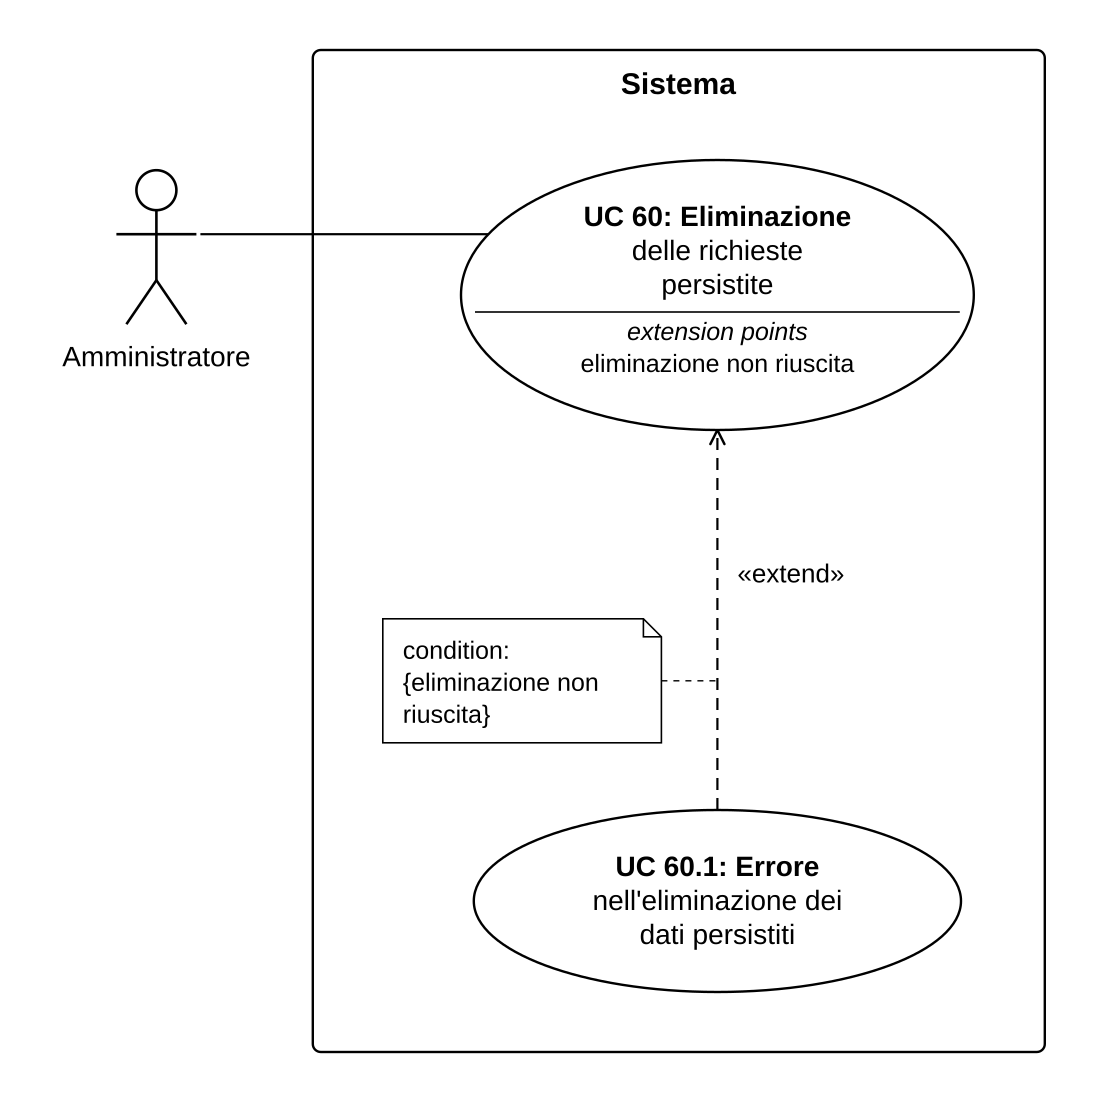
\includegraphics[width=\linewidth,height=0.32\textheight,keepaspectratio]{img/UC60.png}
\caption{UC 60 -- Eliminazione delle richieste persistite}
\end{center}
\begin{itemize}
    \item \textbf{Attore principale}: Amministratore
    \item \textbf{Precondizioni}: L'Amministratore è autenticato.
    \item \textbf{Scenario principale}:
    \begin{enumerate}
        \item L'Amministratore seleziona le richieste persistite da eliminare.
        \item L'Amministratore conferma l'eliminazione.
        \item Il sistema elimina le richieste.
    \end{enumerate}
    \item \textbf{Postcondizioni}: Le richieste selezionate sono eliminate.
    \item \textbf{Trigger}: L'Amministratore vuole liberare la persistenza locale.
    \item \textbf{Estensioni}:
    \begin{itemize}
        \item \hyperref[uc:60.1]{UC 60.1}: Errore nell'eliminazione dei dati persistiti $\rightarrow$ Condizione: Eliminazione non riuscita.
    \end{itemize}
\end{itemize}

\subsubsection{UC 60.1: Errore nell'eliminazione dei dati persistiti}\label{uc:60.1}
\begin{center}
\captionsetup{type=figure}
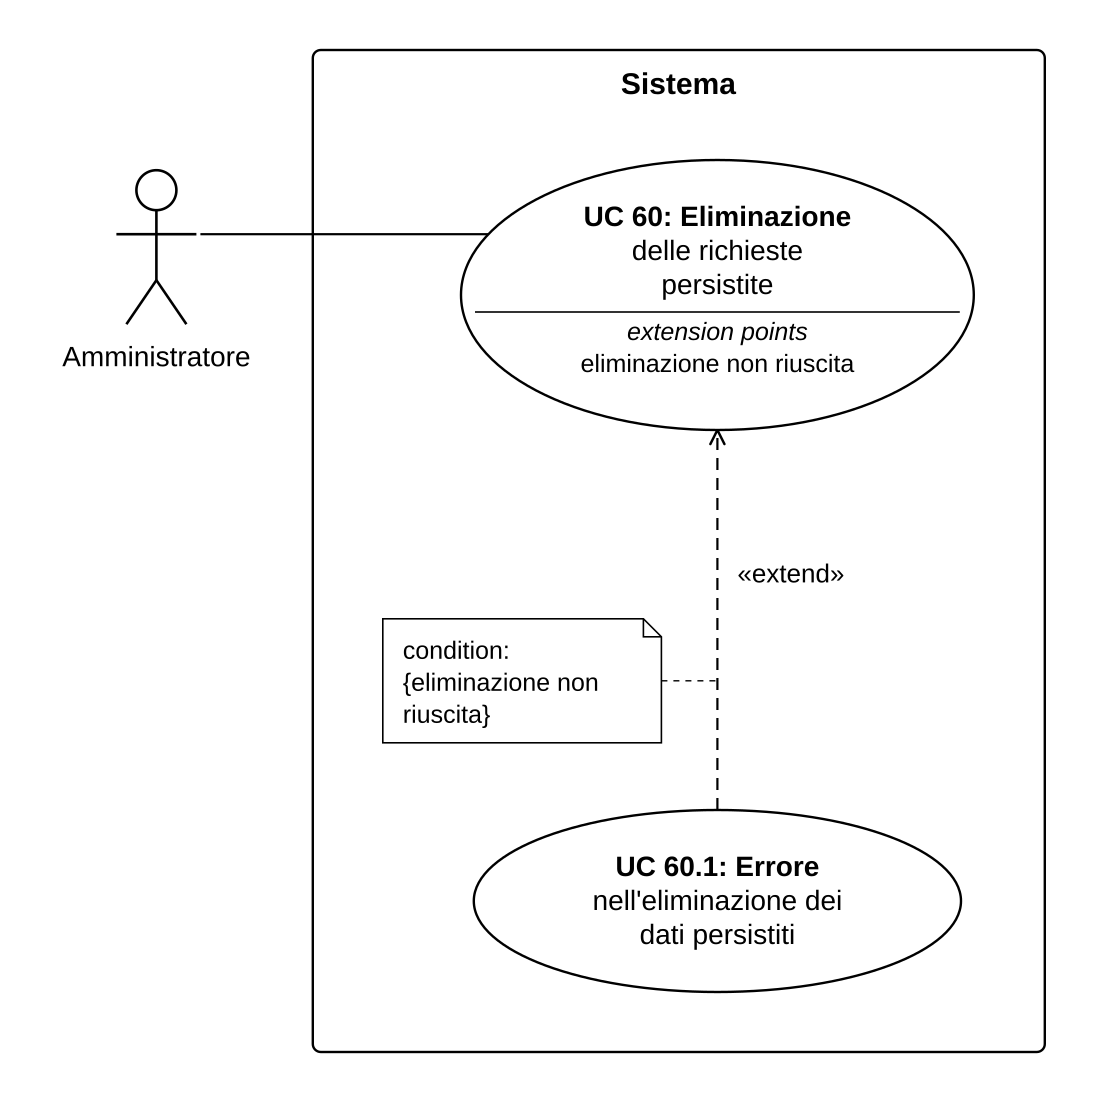
\includegraphics[width=\linewidth,height=0.32\textheight,keepaspectratio]{img/UC60_1.png}
\caption{UC 60.1 -- Errore nell'eliminazione dei dati persistiti}
\end{center}
\begin{itemize}
    \item \textbf{Attore principale}: Amministratore
    \item \textbf{Precondizioni}: L'eliminazione dei dati è in corso.
    \item \textbf{Scenario principale}:
    \begin{enumerate}
        \item Il sistema rileva un errore nell'eliminazione.
        \item Il sistema segnala l'errore all'Amministratore.
    \end{enumerate}
    \item \textbf{Postcondizioni}: I dati non eliminati restano invariati.
    \item \textbf{Trigger}: Eliminazione non riuscita.
    \item \textbf{Estende}: \hyperref[uc:60]{UC 60}.
\end{itemize}

% ------------------------------------------------------------
% MACROAREA 7 --- FUNZIONALITA' OPZIONALI ED ESTENSIONI
% ------------------------------------------------------------
\subsection{Macroarea 7 --- Funzionalità opzionali ed estensioni}

\subsubsection{UC 61: Instradamento di una richiesta non riuscita nella coda di revisione umana}\label{uc:61}
\begin{center}
\captionsetup{type=figure}
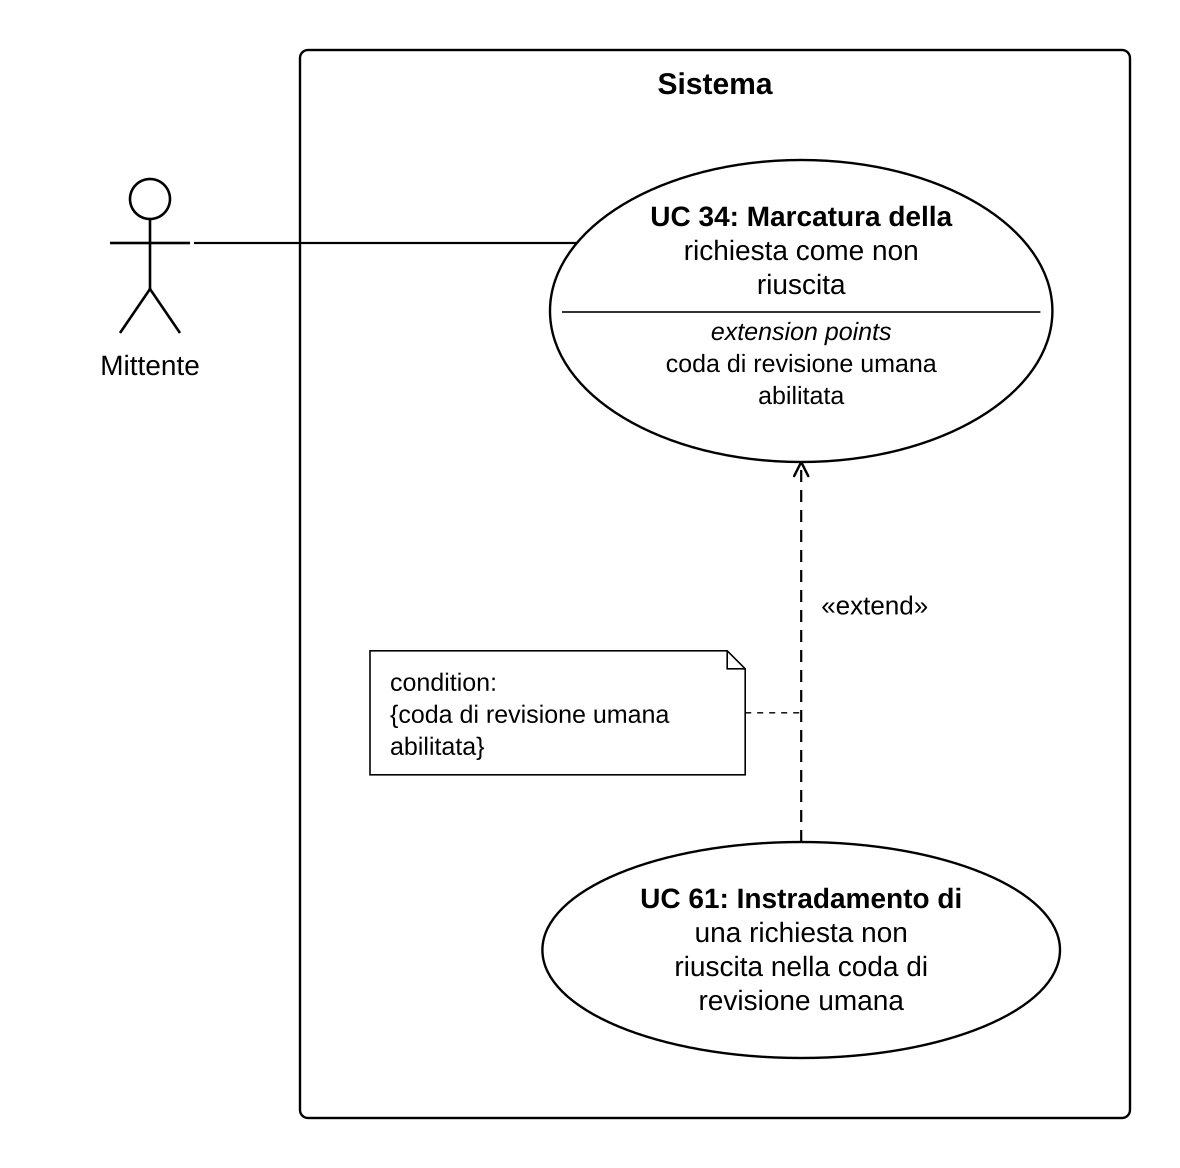
\includegraphics[width=\linewidth,height=0.32\textheight,keepaspectratio]{img/UC61.png}
\caption{UC 61 -- Instradamento di una richiesta non riuscita nella coda di revisione umana}
\end{center}
\begin{itemize}
    \item \textbf{Attore principale}: Mittente
    \item \textbf{Precondizioni}: La revisione umana è abilitata e una richiesta è stata marcata come non riuscita.
    \item \textbf{Scenario principale}:
    \begin{enumerate}
        \item Il sistema instrada la richiesta nella coda di revisione umana.
        \item Il sistema indica motivo ed elemento problematico.
    \end{enumerate}
    \item \textbf{Postcondizioni}: La richiesta è in coda di revisione.
    \item \textbf{Trigger}: Richiesta non riuscita con revisione abilitata.
    \item \textbf{Estende}: \hyperref[uc:34]{UC 34}.
\end{itemize}

\subsubsection{UC 62: Visualizzazione della coda di revisione umana}\label{uc:62}
\begin{center}
\captionsetup{type=figure}
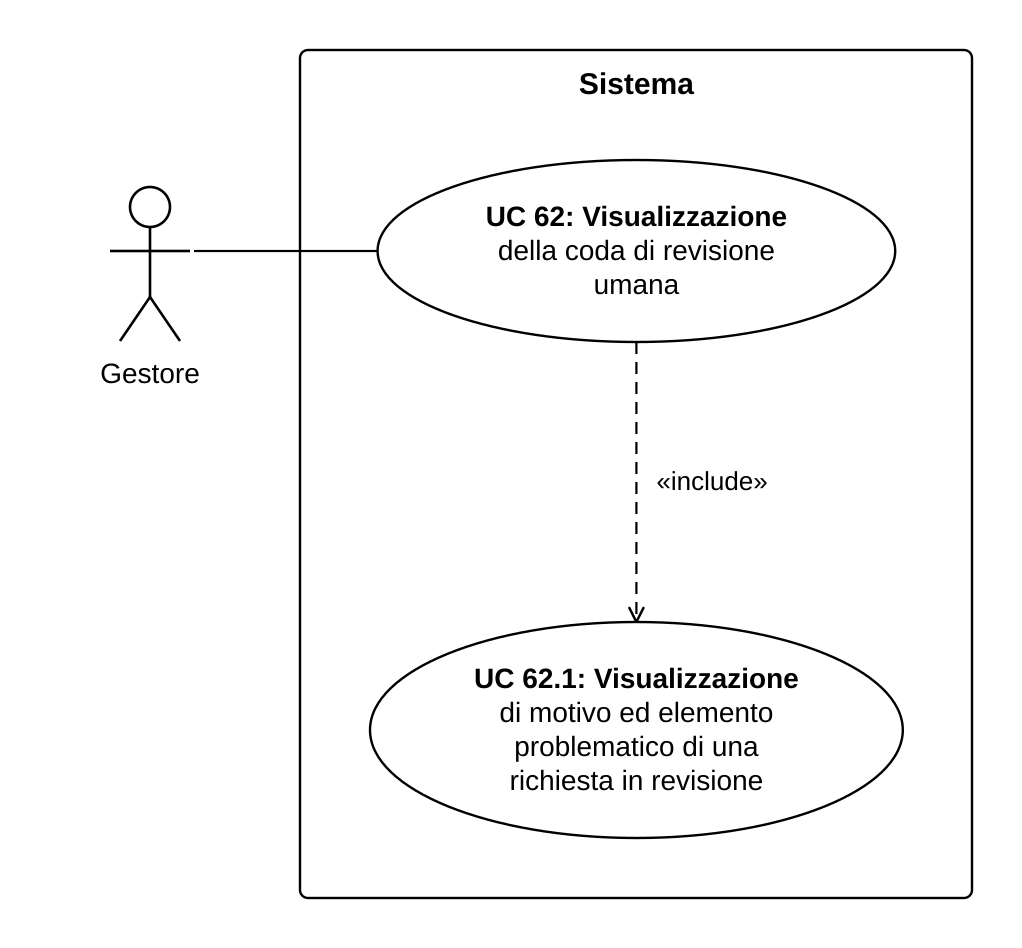
\includegraphics[width=\linewidth,height=0.32\textheight,keepaspectratio]{img/UC62.png}
\caption{UC 62 -- Visualizzazione della coda di revisione umana}
\end{center}
\begin{itemize}
    \item \textbf{Attore principale}: Gestore
    \item \textbf{Precondizioni}: Il Gestore è autenticato.
    \item \textbf{Scenario principale}:
    \begin{enumerate}
        \item Il Gestore apre la coda di revisione.
        \item Il sistema mostra le richieste in revisione.
    \end{enumerate}
    \item \textbf{Postcondizioni}: La coda è visualizzata.
    \item \textbf{Trigger}: Il Gestore vuole esaminare le richieste in revisione.
    \item \textbf{Inclusioni}:
    \begin{itemize}
        \item \hyperref[uc:62.1]{UC 62.1}: Visualizzazione di motivo ed elemento problematico di una richiesta in revisione
    \end{itemize}
\end{itemize}

\subsubsection{UC 62.1: Visualizzazione di motivo ed elemento problematico di una richiesta in revisione}\label{uc:62.1}
\begin{center}
\captionsetup{type=figure}
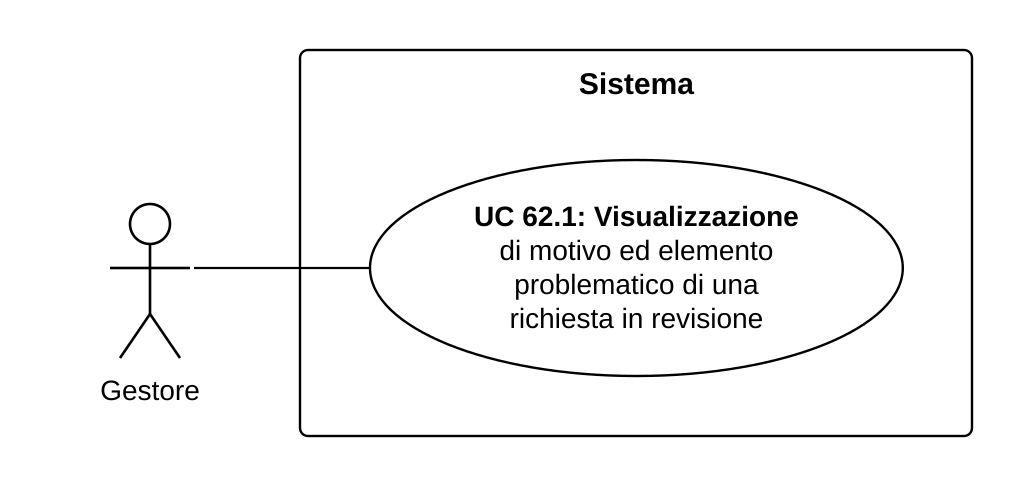
\includegraphics[width=\linewidth,height=0.32\textheight,keepaspectratio]{img/UC62_1.png}
\caption{UC 62.1 -- Visualizzazione di motivo ed elemento problematico di una richiesta in revisione}
\end{center}
\begin{itemize}
    \item \textbf{Attore principale}: Gestore
    \item \textbf{Precondizioni}: La coda di revisione è visualizzata.
    \item \textbf{Scenario principale}:
    \begin{enumerate}
        \item Il Gestore seleziona una richiesta.
        \item Il sistema mostra il motivo dell'anomalia e l'elemento segnalato.
    \end{enumerate}
    \item \textbf{Postcondizioni}: Motivo ed elemento sono visualizzati.
    \item \textbf{Trigger}: Il Gestore vuole capire l'anomalia.
    \item \textbf{Incluso da}: \hyperref[uc:62]{UC 62}.
\end{itemize}

\subsubsection{UC 63: Correzione o completamento dei dati di una richiesta in revisione}\label{uc:63}
\begin{center}
\captionsetup{type=figure}
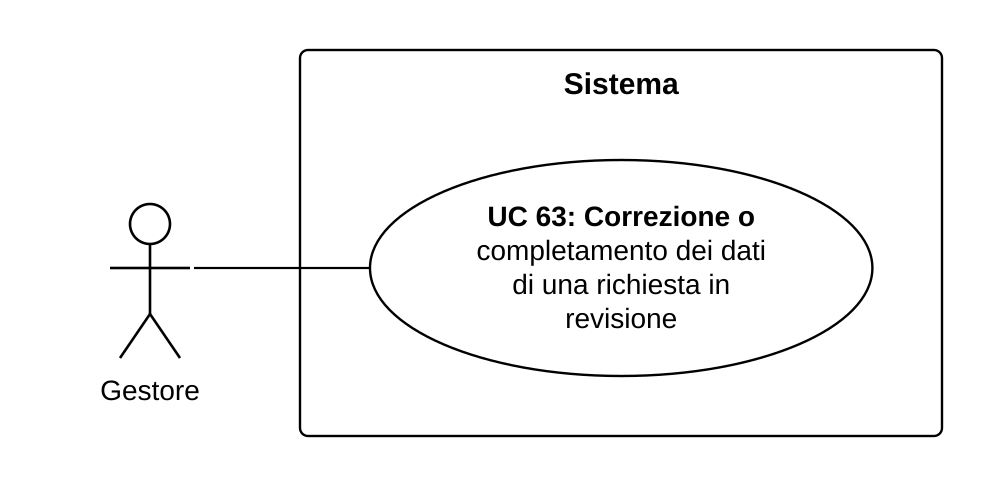
\includegraphics[width=\linewidth,height=0.32\textheight,keepaspectratio]{img/UC63.png}
\caption{UC 63 -- Correzione o completamento dei dati di una richiesta in revisione}
\end{center}
\begin{itemize}
    \item \textbf{Attore principale}: Gestore
    \item \textbf{Precondizioni}: Il Gestore è autenticato e una richiesta è in revisione.
    \item \textbf{Scenario principale}:
    \begin{enumerate}
        \item Il Gestore apre la richiesta.
        \item Il Gestore corregge o completa i dati.
        \item Il sistema salva le modifiche.
    \end{enumerate}
    \item \textbf{Postcondizioni}: I dati della richiesta sono corretti.
    \item \textbf{Trigger}: Il Gestore vuole sistemare una richiesta.
\end{itemize}

\subsubsection{UC 64: Approvazione di una richiesta revisionata}\label{uc:64}
\begin{center}
\captionsetup{type=figure}
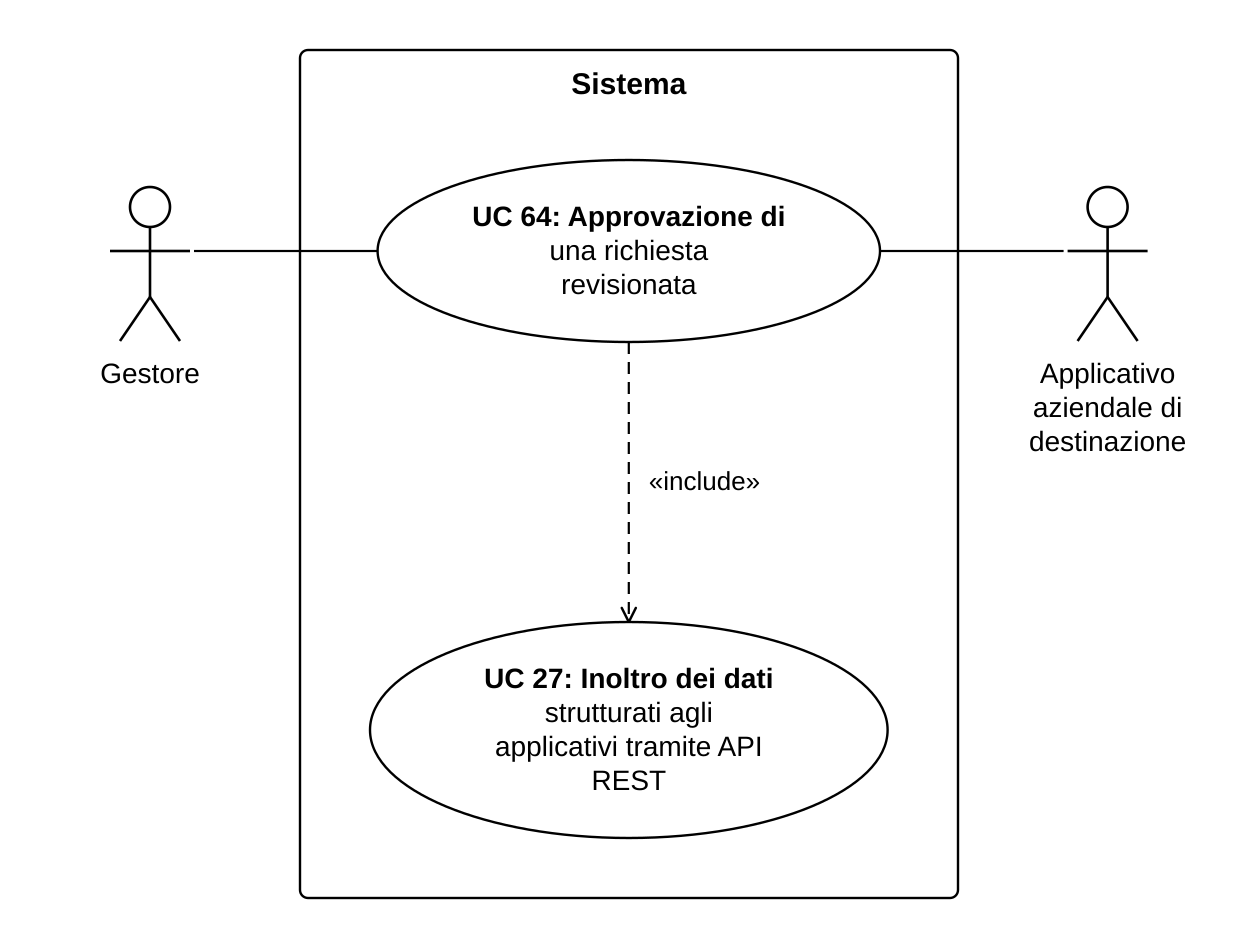
\includegraphics[width=\linewidth,height=0.32\textheight,keepaspectratio]{img/UC64.png}
\caption{UC 64 -- Approvazione di una richiesta revisionata}
\end{center}
\begin{itemize}
    \item \textbf{Attore principale}: Gestore
    \item \textbf{Attori secondari}: Applicativo aziendale di destinazione
    \item \textbf{Precondizioni}: Il Gestore è autenticato e una richiesta in revisione è stata corretta.
    \item \textbf{Scenario principale}:
    \begin{enumerate}
        \item Il Gestore approva la richiesta.
        \item Il sistema avvia l'inoltro automatico (\hyperref[uc:27]{UC 27}).
    \end{enumerate}
    \item \textbf{Postcondizioni}: La richiesta è inoltrata.
    \item \textbf{Trigger}: Il Gestore vuole confermare la richiesta.
    \item \textbf{Inclusioni}:
    \begin{itemize}
        \item \hyperref[uc:27]{UC 27}: Inoltro dei dati strutturati agli applicativi tramite API REST
    \end{itemize}
\end{itemize}

\subsubsection{UC 65: Scarto di una richiesta in revisione}\label{uc:65}
\begin{center}
\captionsetup{type=figure}
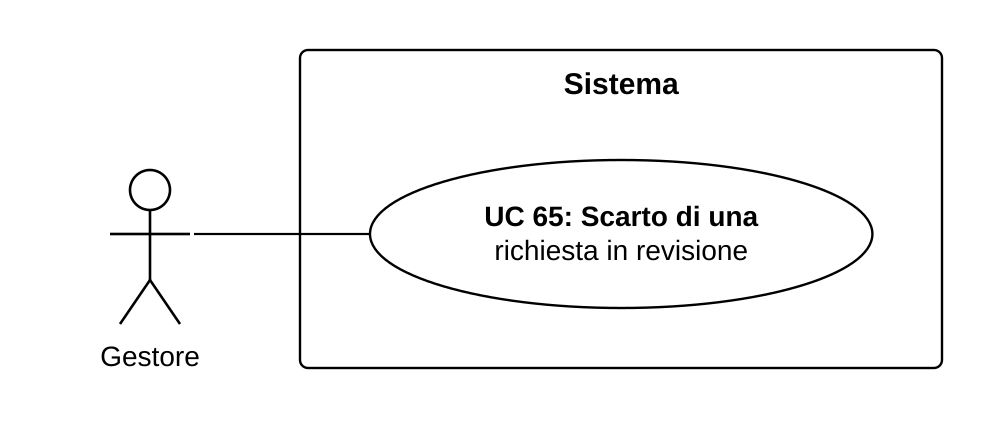
\includegraphics[width=\linewidth,height=0.32\textheight,keepaspectratio]{img/UC65.png}
\caption{UC 65 -- Scarto di una richiesta in revisione}
\end{center}
\begin{itemize}
    \item \textbf{Attore principale}: Gestore
    \item \textbf{Precondizioni}: Il Gestore è autenticato e una richiesta è in revisione.
    \item \textbf{Scenario principale}:
    \begin{enumerate}
        \item Il Gestore sceglie di scartare la richiesta.
        \item Il Gestore indica il motivo.
        \item Il sistema scarta la richiesta e traccia il motivo.
    \end{enumerate}
    \item \textbf{Postcondizioni}: La richiesta è scartata con motivo.
    \item \textbf{Trigger}: Il Gestore vuole scartare la richiesta.
\end{itemize}

\subsubsection{UC 66: Visualizzazione della dashboard analitica}\label{uc:66}
\begin{center}
\captionsetup{type=figure}
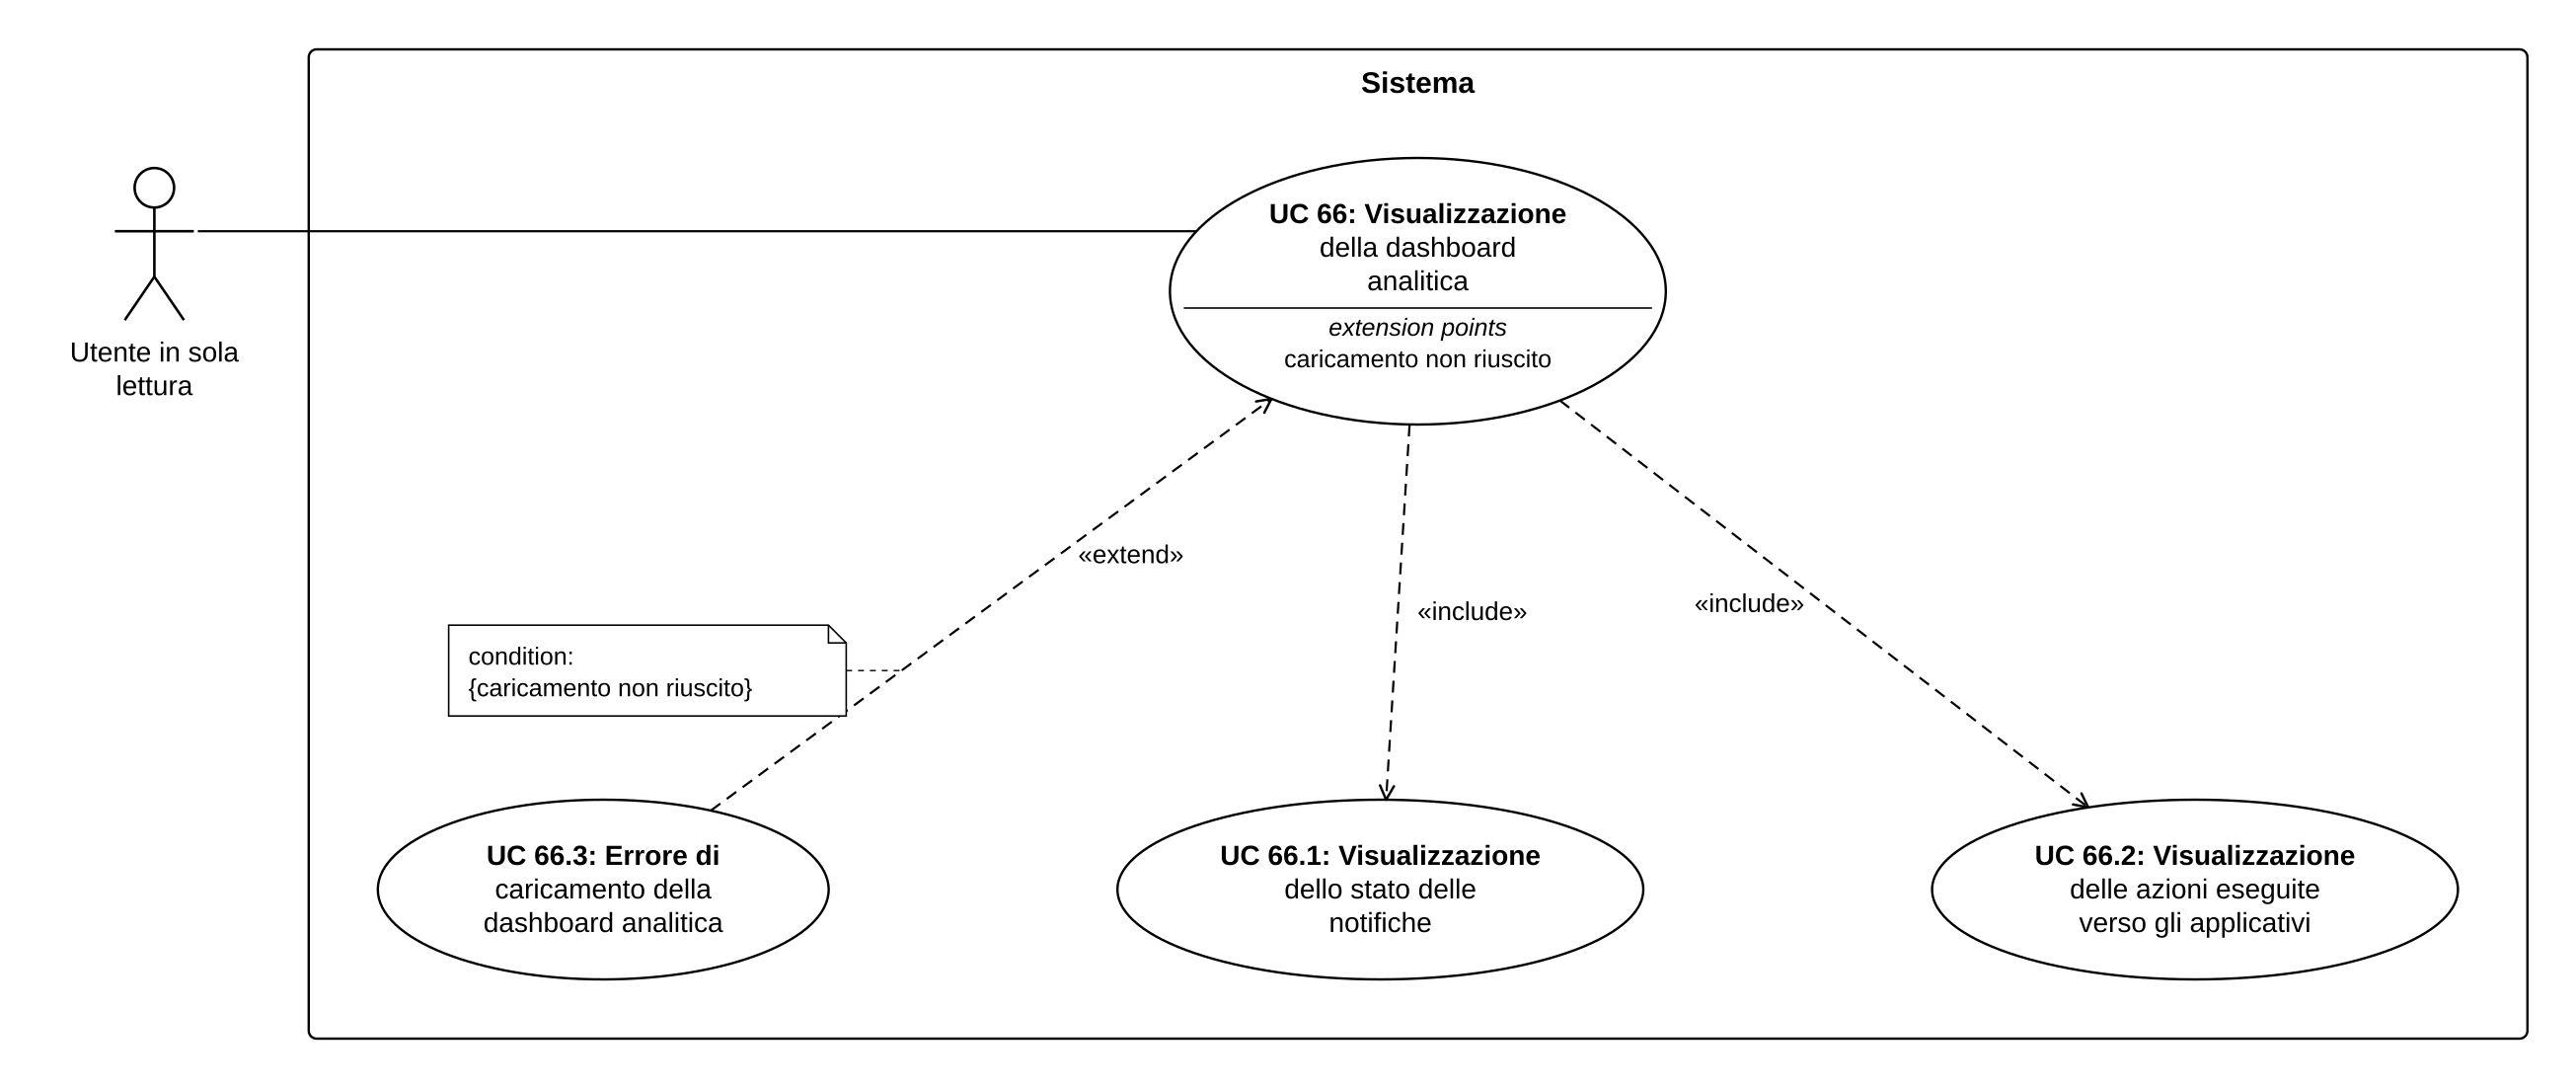
\includegraphics[width=\linewidth,height=0.32\textheight,keepaspectratio]{img/UC66.png}
\caption{UC 66 -- Visualizzazione della dashboard analitica}
\end{center}
\begin{itemize}
    \item \textbf{Attore principale}: Utente in sola lettura
    \item \textbf{Precondizioni}: L'utente è autenticato.
    \item \textbf{Scenario principale}:
    \begin{enumerate}
        \item L'utente apre la dashboard analitica.
        \item Il sistema mostra la sintesi dei flussi di lavoro.
    \end{enumerate}
    \item \textbf{Postcondizioni}: La dashboard è visualizzata.
    \item \textbf{Trigger}: L'utente vuole una vista sintetica dei flussi.
    \item \textbf{Inclusioni}:
    \begin{itemize}
        \item \hyperref[uc:66.1]{UC 66.1}: Visualizzazione dello stato delle notifiche
        \item \hyperref[uc:66.2]{UC 66.2}: Visualizzazione delle azioni eseguite verso gli applicativi
    \end{itemize}
    \item \textbf{Estensioni}:
    \begin{itemize}
        \item \hyperref[uc:66.3]{UC 66.3}: Errore di caricamento della dashboard analitica $\rightarrow$ Condizione: Caricamento non riuscito.
    \end{itemize}
\end{itemize}

\subsubsection{UC 66.1: Visualizzazione dello stato delle notifiche}\label{uc:66.1}
\begin{center}
\captionsetup{type=figure}
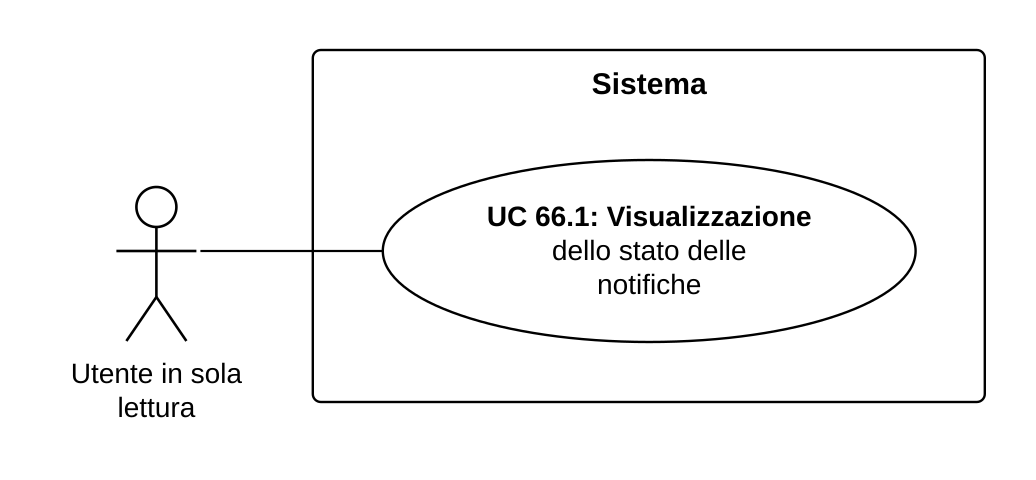
\includegraphics[width=\linewidth,height=0.32\textheight,keepaspectratio]{img/UC66_1.png}
\caption{UC 66.1 -- Visualizzazione dello stato delle notifiche}
\end{center}
\begin{itemize}
    \item \textbf{Attore principale}: Utente in sola lettura
    \item \textbf{Precondizioni}: La dashboard analitica è in caricamento.
    \item \textbf{Scenario principale}:
    \begin{enumerate}
        \item Il sistema mostra lo stato delle notifiche.
    \end{enumerate}
    \item \textbf{Postcondizioni}: Lo stato delle notifiche è visualizzato.
    \item \textbf{Trigger}: Apertura della dashboard.
    \item \textbf{Incluso da}: \hyperref[uc:66]{UC 66}.
\end{itemize}

\subsubsection{UC 66.2: Visualizzazione delle azioni eseguite verso gli applicativi}\label{uc:66.2}
\begin{center}
\captionsetup{type=figure}
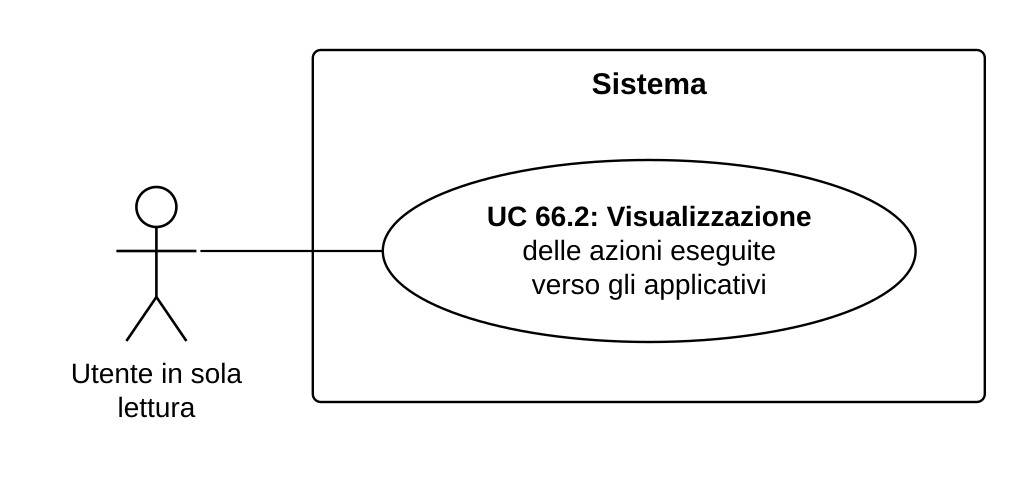
\includegraphics[width=\linewidth,height=0.32\textheight,keepaspectratio]{img/UC66_2.png}
\caption{UC 66.2 -- Visualizzazione delle azioni eseguite verso gli applicativi}
\end{center}
\begin{itemize}
    \item \textbf{Attore principale}: Utente in sola lettura
    \item \textbf{Precondizioni}: La dashboard analitica è in caricamento.
    \item \textbf{Scenario principale}:
    \begin{enumerate}
        \item Il sistema mostra le azioni eseguite verso gli applicativi.
    \end{enumerate}
    \item \textbf{Postcondizioni}: Le azioni sono visualizzate.
    \item \textbf{Trigger}: Apertura della dashboard.
    \item \textbf{Incluso da}: \hyperref[uc:66]{UC 66}.
\end{itemize}

\subsubsection{UC 66.3: Errore di caricamento della dashboard analitica}\label{uc:66.3}
\begin{center}
\captionsetup{type=figure}
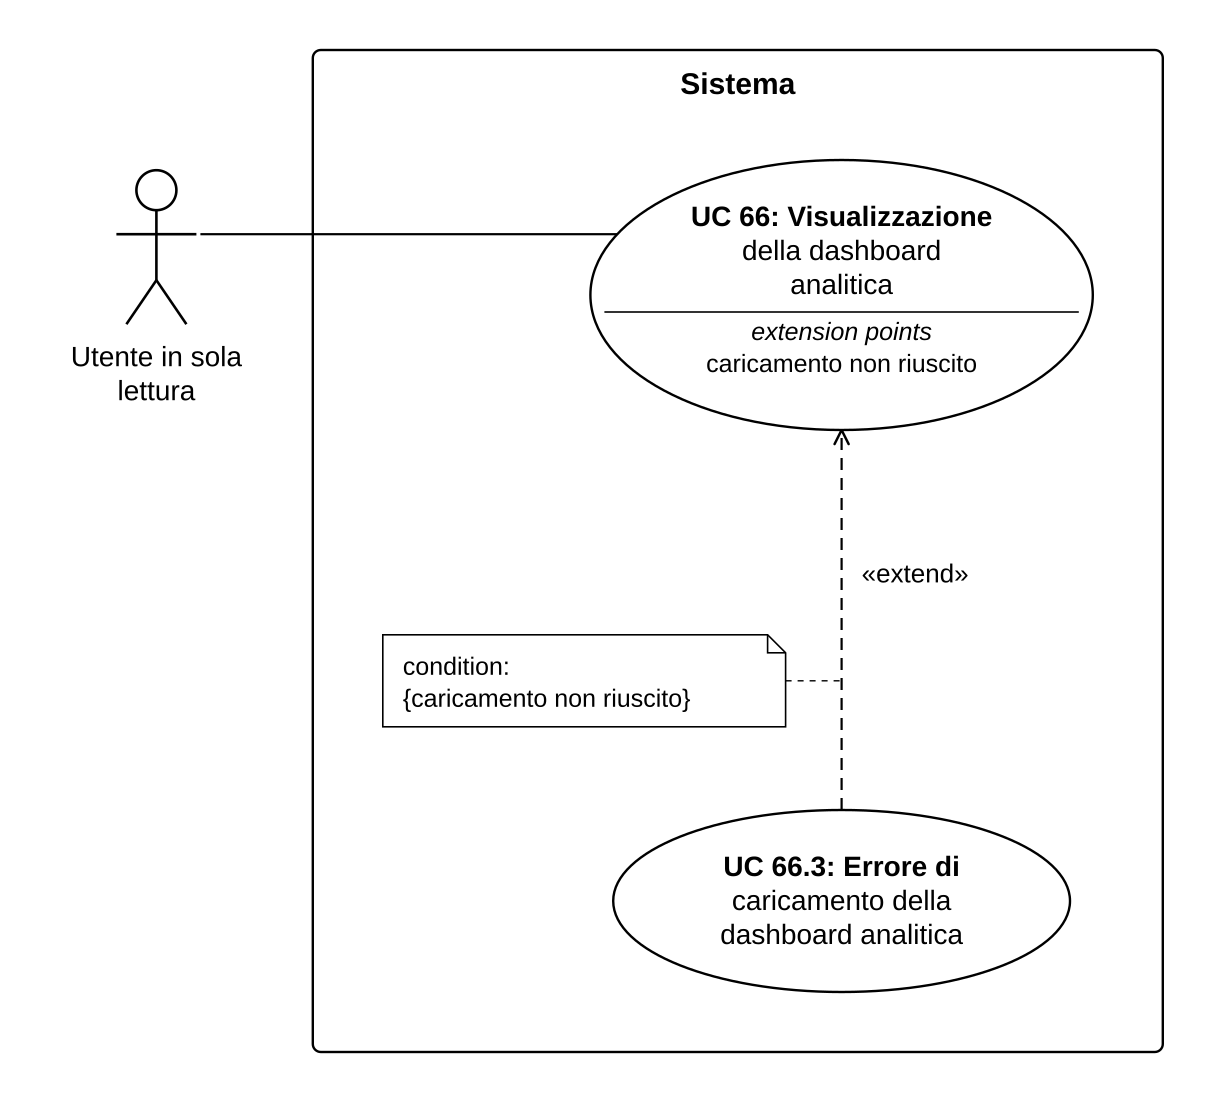
\includegraphics[width=\linewidth,height=0.32\textheight,keepaspectratio]{img/UC66_3.png}
\caption{UC 66.3 -- Errore di caricamento della dashboard analitica}
\end{center}
\begin{itemize}
    \item \textbf{Attore principale}: Utente in sola lettura
    \item \textbf{Precondizioni}: Il caricamento della dashboard è in corso.
    \item \textbf{Scenario principale}:
    \begin{enumerate}
        \item Il sistema rileva un errore di caricamento.
        \item Il sistema segnala l'errore all'utente.
    \end{enumerate}
    \item \textbf{Postcondizioni}: La dashboard non è visualizzata.
    \item \textbf{Trigger}: Caricamento non riuscito.
    \item \textbf{Estende}: \hyperref[uc:66]{UC 66}.
\end{itemize}

\subsubsection{UC 67: Invio al mittente della conferma di ricezione}\label{uc:67}
\begin{center}
\captionsetup{type=figure}
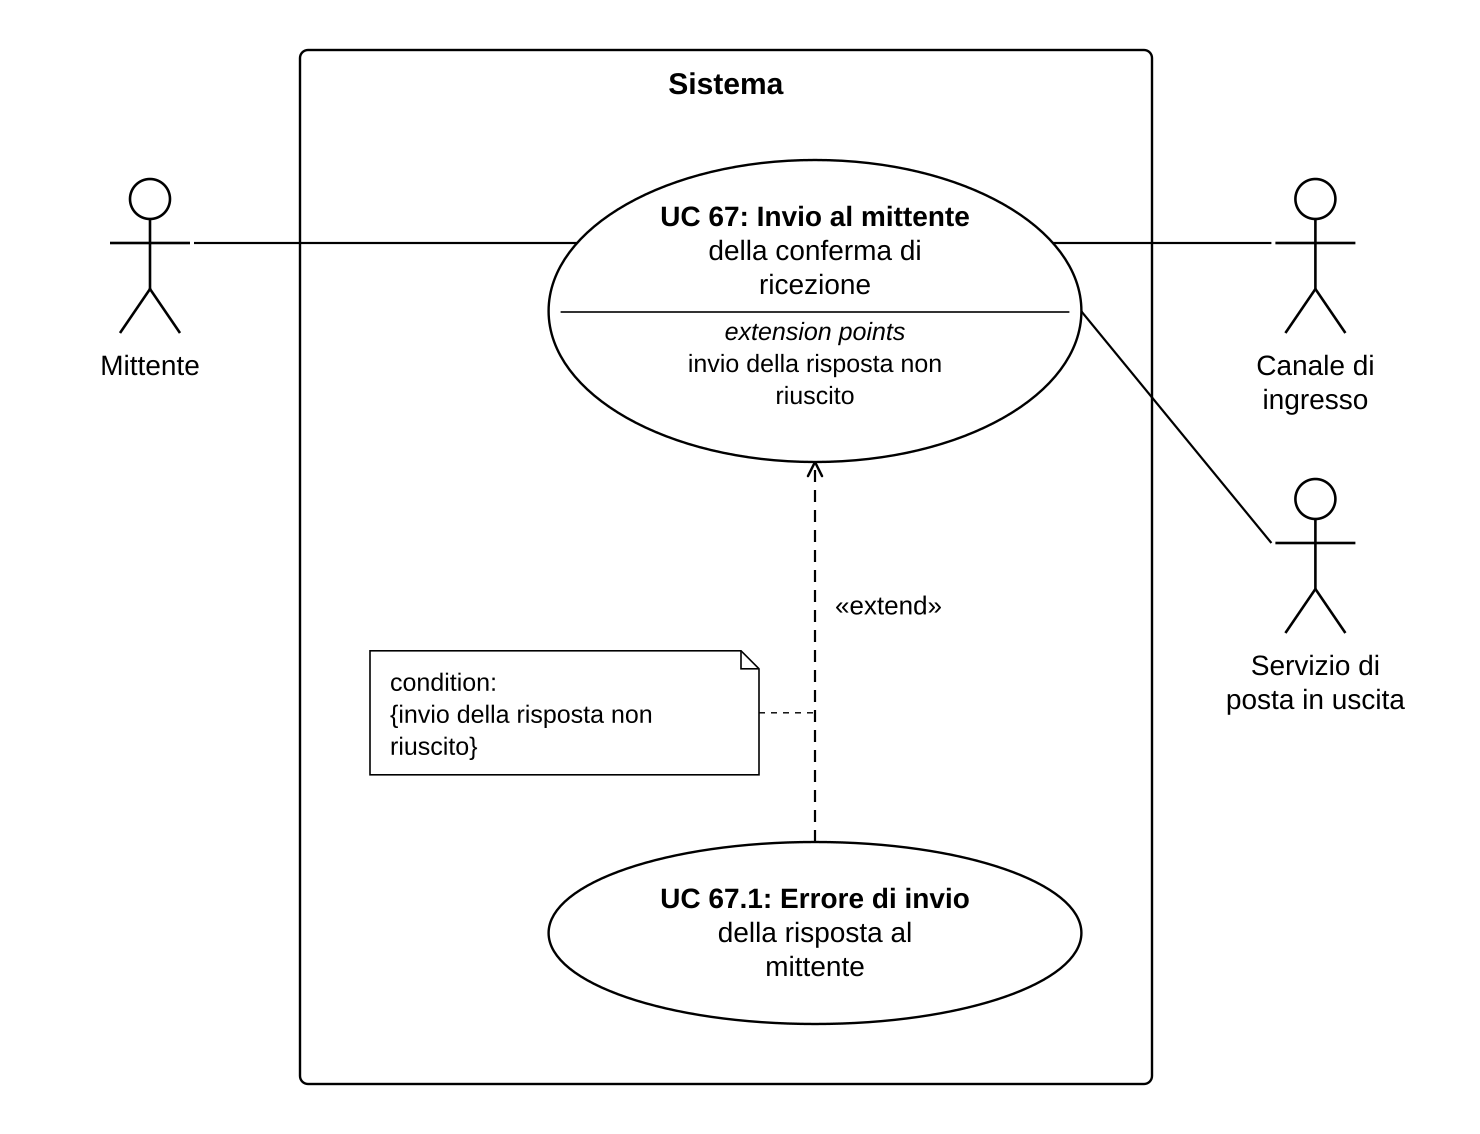
\includegraphics[width=\linewidth,height=0.32\textheight,keepaspectratio]{img/UC67.png}
\caption{UC 67 -- Invio al mittente della conferma di ricezione}
\end{center}
\begin{itemize}
    \item \textbf{Attore principale}: Mittente
    \item \textbf{Attori secondari}: Canale di ingresso, Servizio di posta in uscita
    \item \textbf{Precondizioni}: Una richiesta è stata ricevuta correttamente.
    \item \textbf{Scenario principale}:
    \begin{enumerate}
        \item Il sistema compone la conferma di ricezione.
        \item Il sistema la invia al mittente via e-mail o messaggio, secondo il canale.
    \end{enumerate}
    \item \textbf{Postcondizioni}: Il mittente ha ricevuto la conferma.
    \item \textbf{Trigger}: Ricezione di una richiesta.
    \item \textbf{Estensioni}:
    \begin{itemize}
        \item \hyperref[uc:67.1]{UC 67.1}: Errore di invio della risposta al mittente $\rightarrow$ Condizione: Invio della risposta non riuscito.
    \end{itemize}
\end{itemize}

\subsubsection{UC 67.1: Errore di invio della risposta al mittente}\label{uc:67.1}
\begin{center}
\captionsetup{type=figure}
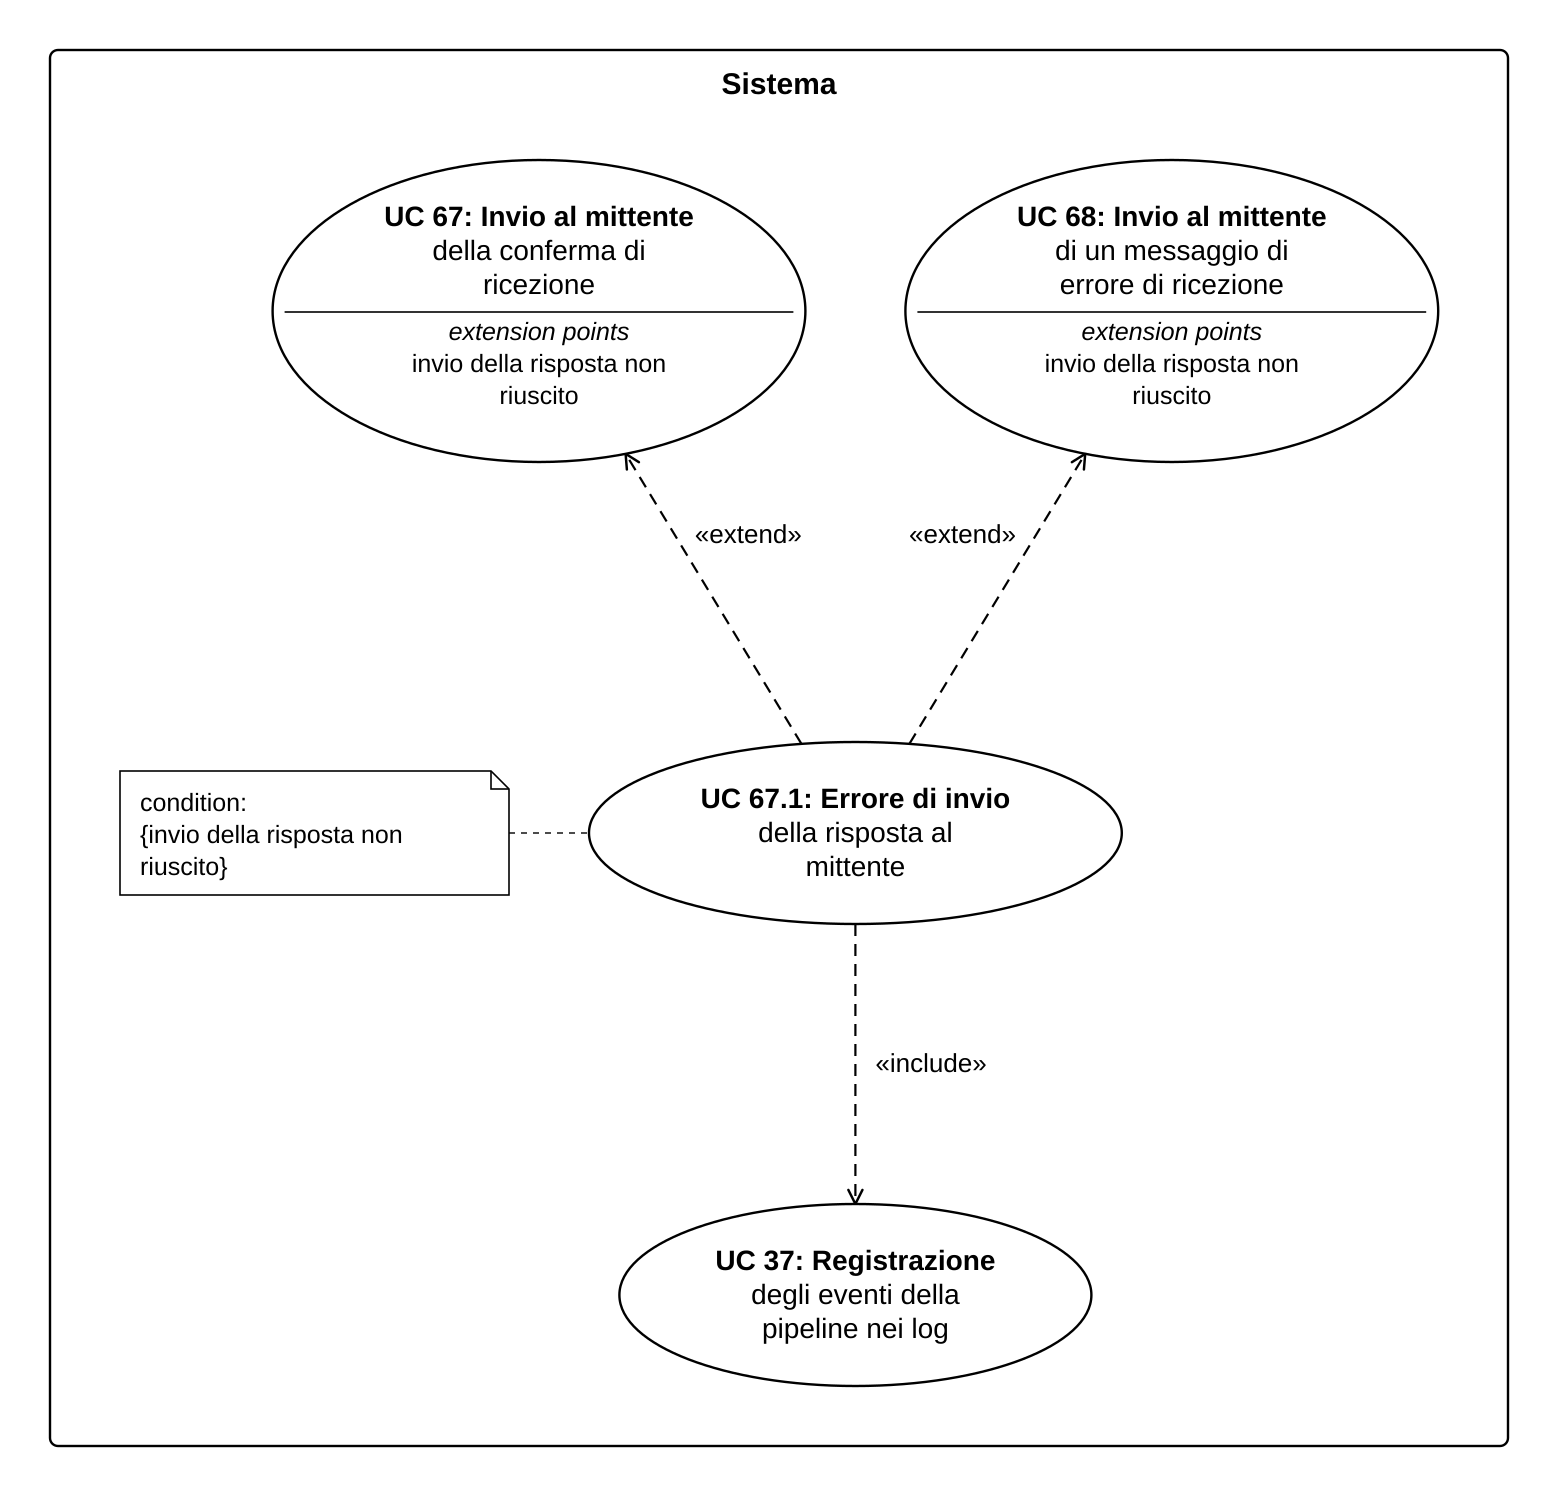
\includegraphics[width=\linewidth,height=0.32\textheight,keepaspectratio]{img/UC67_1.png}
\caption{UC 67.1 -- Errore di invio della risposta al mittente}
\end{center}
\begin{itemize}
    \item \textbf{Attore principale}: Mittente
    \item \textbf{Precondizioni}: L'invio di una risposta al mittente è in corso.
    \item \textbf{Scenario principale}:
    \begin{enumerate}
        \item Il sistema rileva un errore di invio.
        \item Il sistema registra l'errore nei log (\hyperref[uc:37]{UC 37}).
    \end{enumerate}
    \item \textbf{Postcondizioni}: L'errore è registrato nei log.
    \item \textbf{Trigger}: Invio della risposta non riuscito.
    \item \textbf{Estende}: \hyperref[uc:67]{UC 67}, \hyperref[uc:68]{UC 68}.
    \item \textbf{Inclusioni}:
    \begin{itemize}
        \item \hyperref[uc:37]{UC 37}: Registrazione degli eventi della pipeline nei log
    \end{itemize}
\end{itemize}

\subsubsection{UC 68: Invio al mittente di un messaggio di errore di ricezione}\label{uc:68}
\begin{center}
\captionsetup{type=figure}
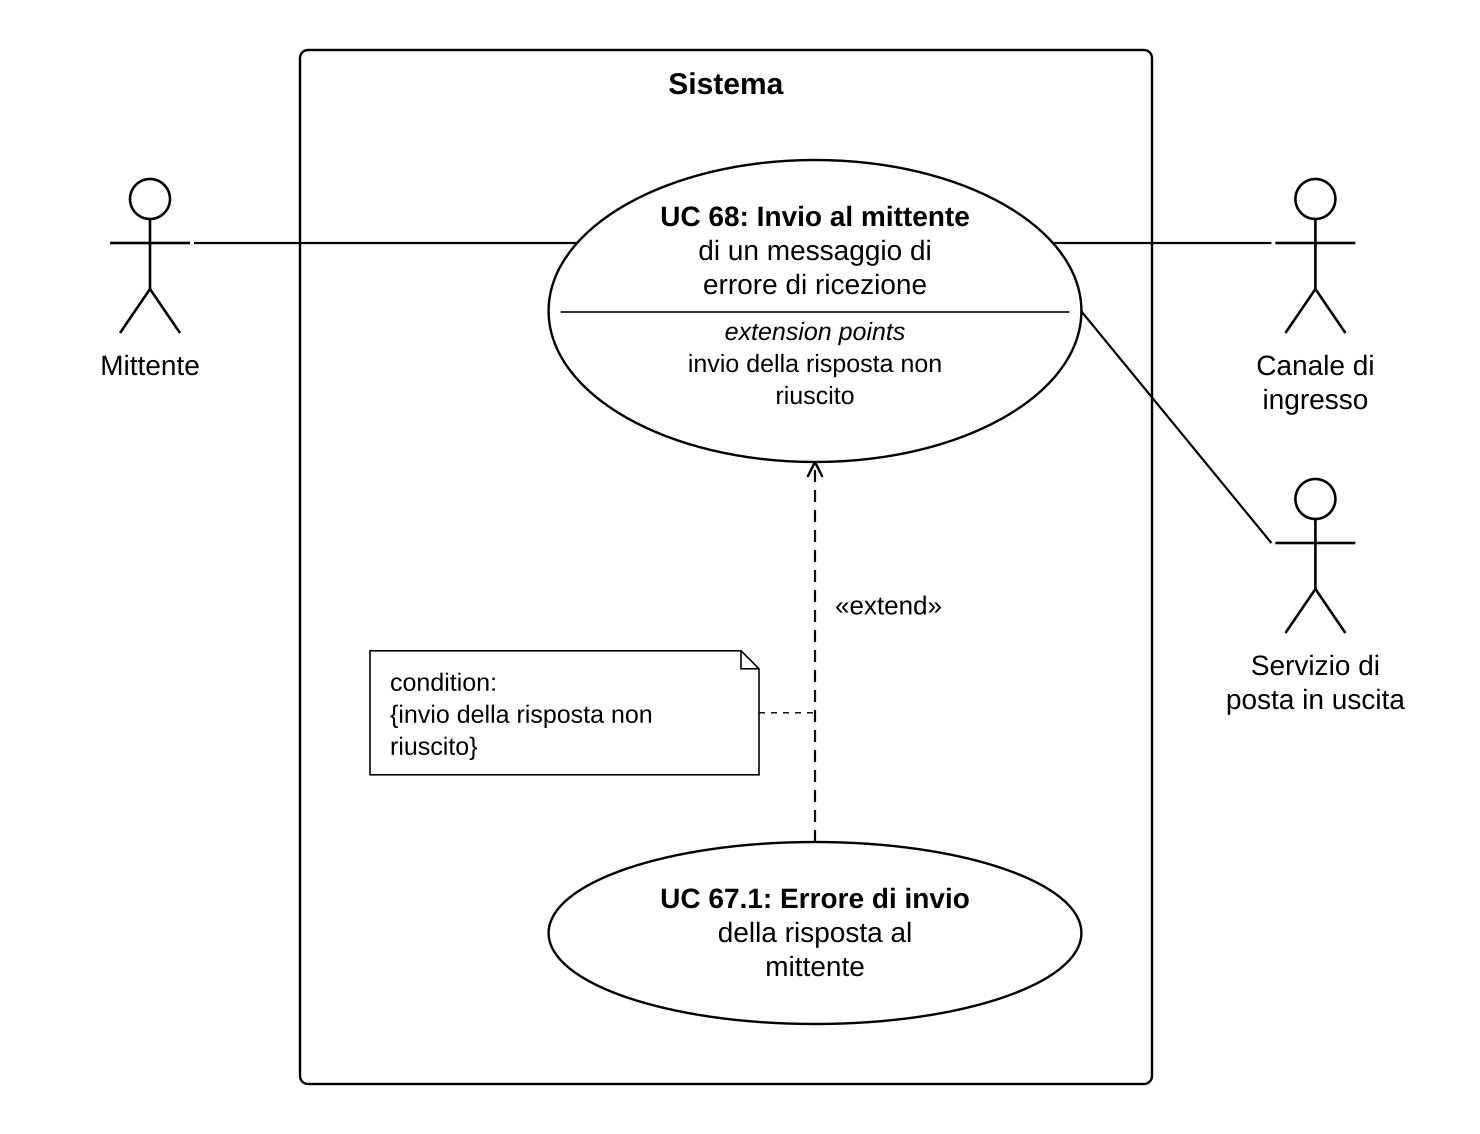
\includegraphics[width=\linewidth,height=0.32\textheight,keepaspectratio]{img/UC68.png}
\caption{UC 68 -- Invio al mittente di un messaggio di errore di ricezione}
\end{center}
\begin{itemize}
    \item \textbf{Attore principale}: Mittente
    \item \textbf{Attori secondari}: Canale di ingresso, Servizio di posta in uscita
    \item \textbf{Precondizioni}: Si è verificato un errore nella ricezione di una richiesta.
    \item \textbf{Scenario principale}:
    \begin{enumerate}
        \item Il sistema compone un messaggio di errore.
        \item Il sistema lo invia al mittente.
    \end{enumerate}
    \item \textbf{Postcondizioni}: Il mittente è informato dell'errore.
    \item \textbf{Trigger}: Errore nella ricezione di una richiesta.
    \item \textbf{Estensioni}:
    \begin{itemize}
        \item \hyperref[uc:67.1]{UC 67.1}: Errore di invio della risposta al mittente $\rightarrow$ Condizione: Invio della risposta non riuscito.
    \end{itemize}
\end{itemize}

\subsubsection{UC 69: Acquisizione di registrazioni e trascrizioni di meeting}\label{uc:69}
\begin{center}
\captionsetup{type=figure}
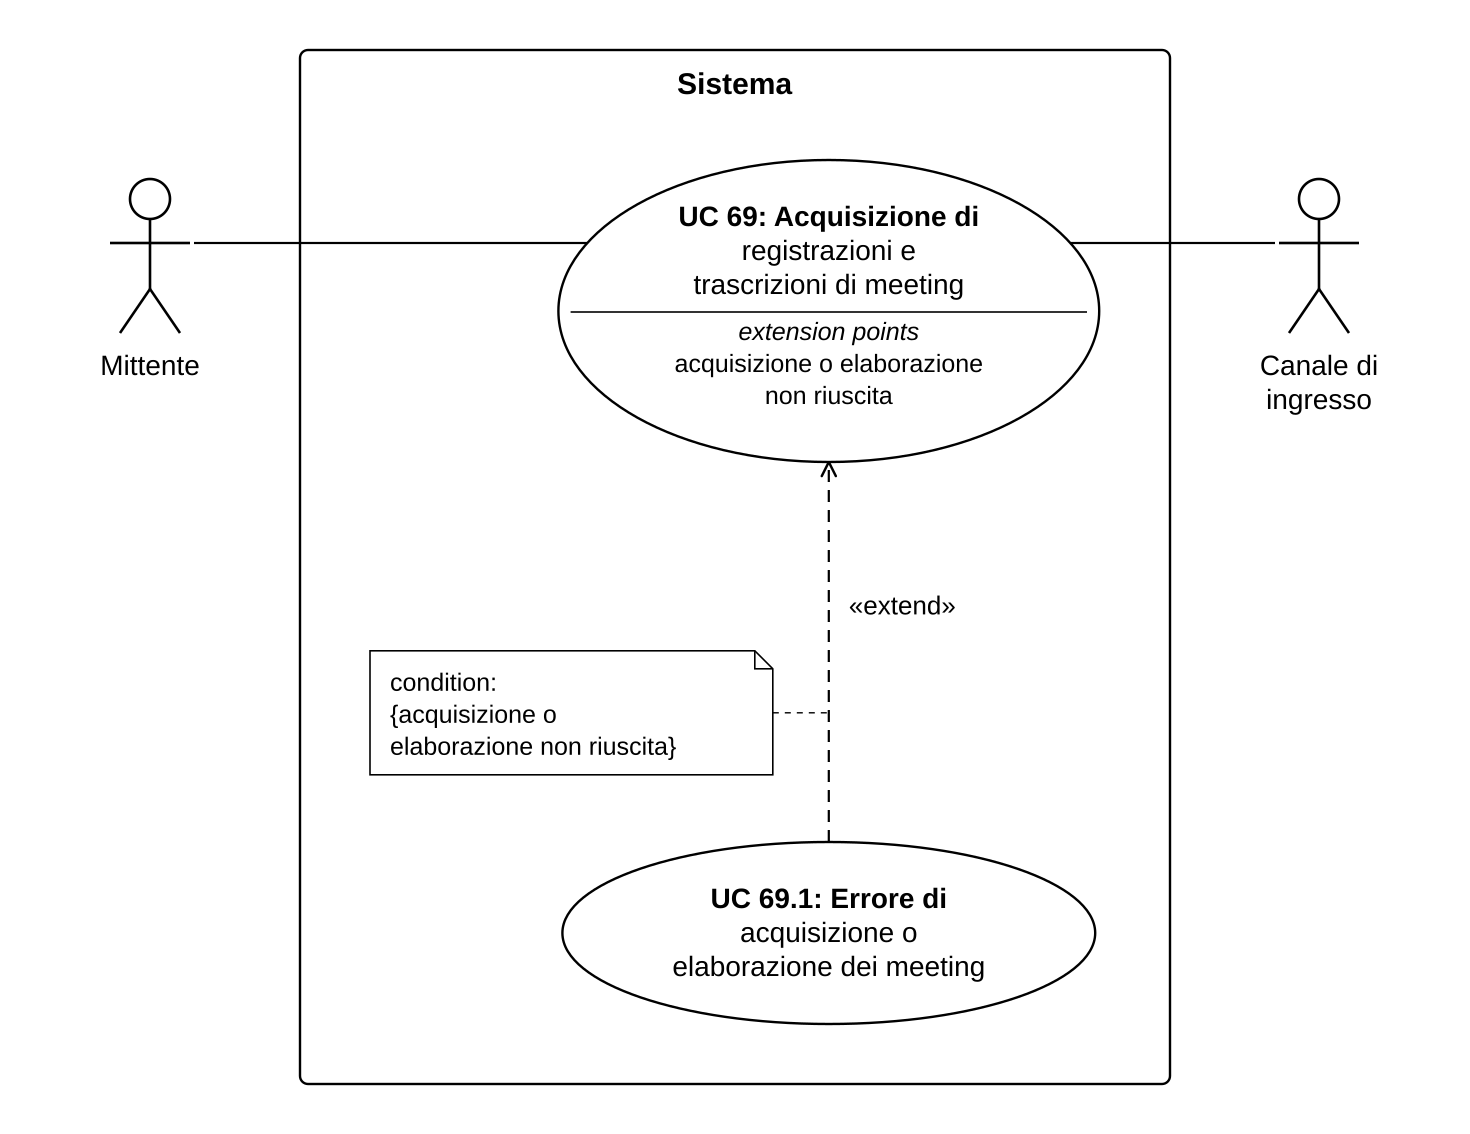
\includegraphics[width=\linewidth,height=0.32\textheight,keepaspectratio]{img/UC69.png}
\caption{UC 69 -- Acquisizione di registrazioni e trascrizioni di meeting}
\end{center}
\begin{itemize}
    \item \textbf{Attore principale}: Mittente
    \item \textbf{Attori secondari}: Canale di ingresso
    \item \textbf{Precondizioni}: Il canale dei meeting è configurato e attivo.
    \item \textbf{Scenario principale}:
    \begin{enumerate}
        \item Il sistema rileva una registrazione o trascrizione di un meeting.
        \item Il sistema la acquisisce e crea una richiesta.
    \end{enumerate}
    \item \textbf{Postcondizioni}: Il meeting è acquisito.
    \item \textbf{Trigger}: Disponibilità di un meeting.
    \item \textbf{Estensioni}:
    \begin{itemize}
        \item \hyperref[uc:69.1]{UC 69.1}: Errore di acquisizione o elaborazione dei meeting $\rightarrow$ Condizione: Acquisizione o elaborazione non riuscita.
    \end{itemize}
\end{itemize}

\subsubsection{UC 69.1: Errore di acquisizione o elaborazione dei meeting}\label{uc:69.1}
\begin{center}
\captionsetup{type=figure}
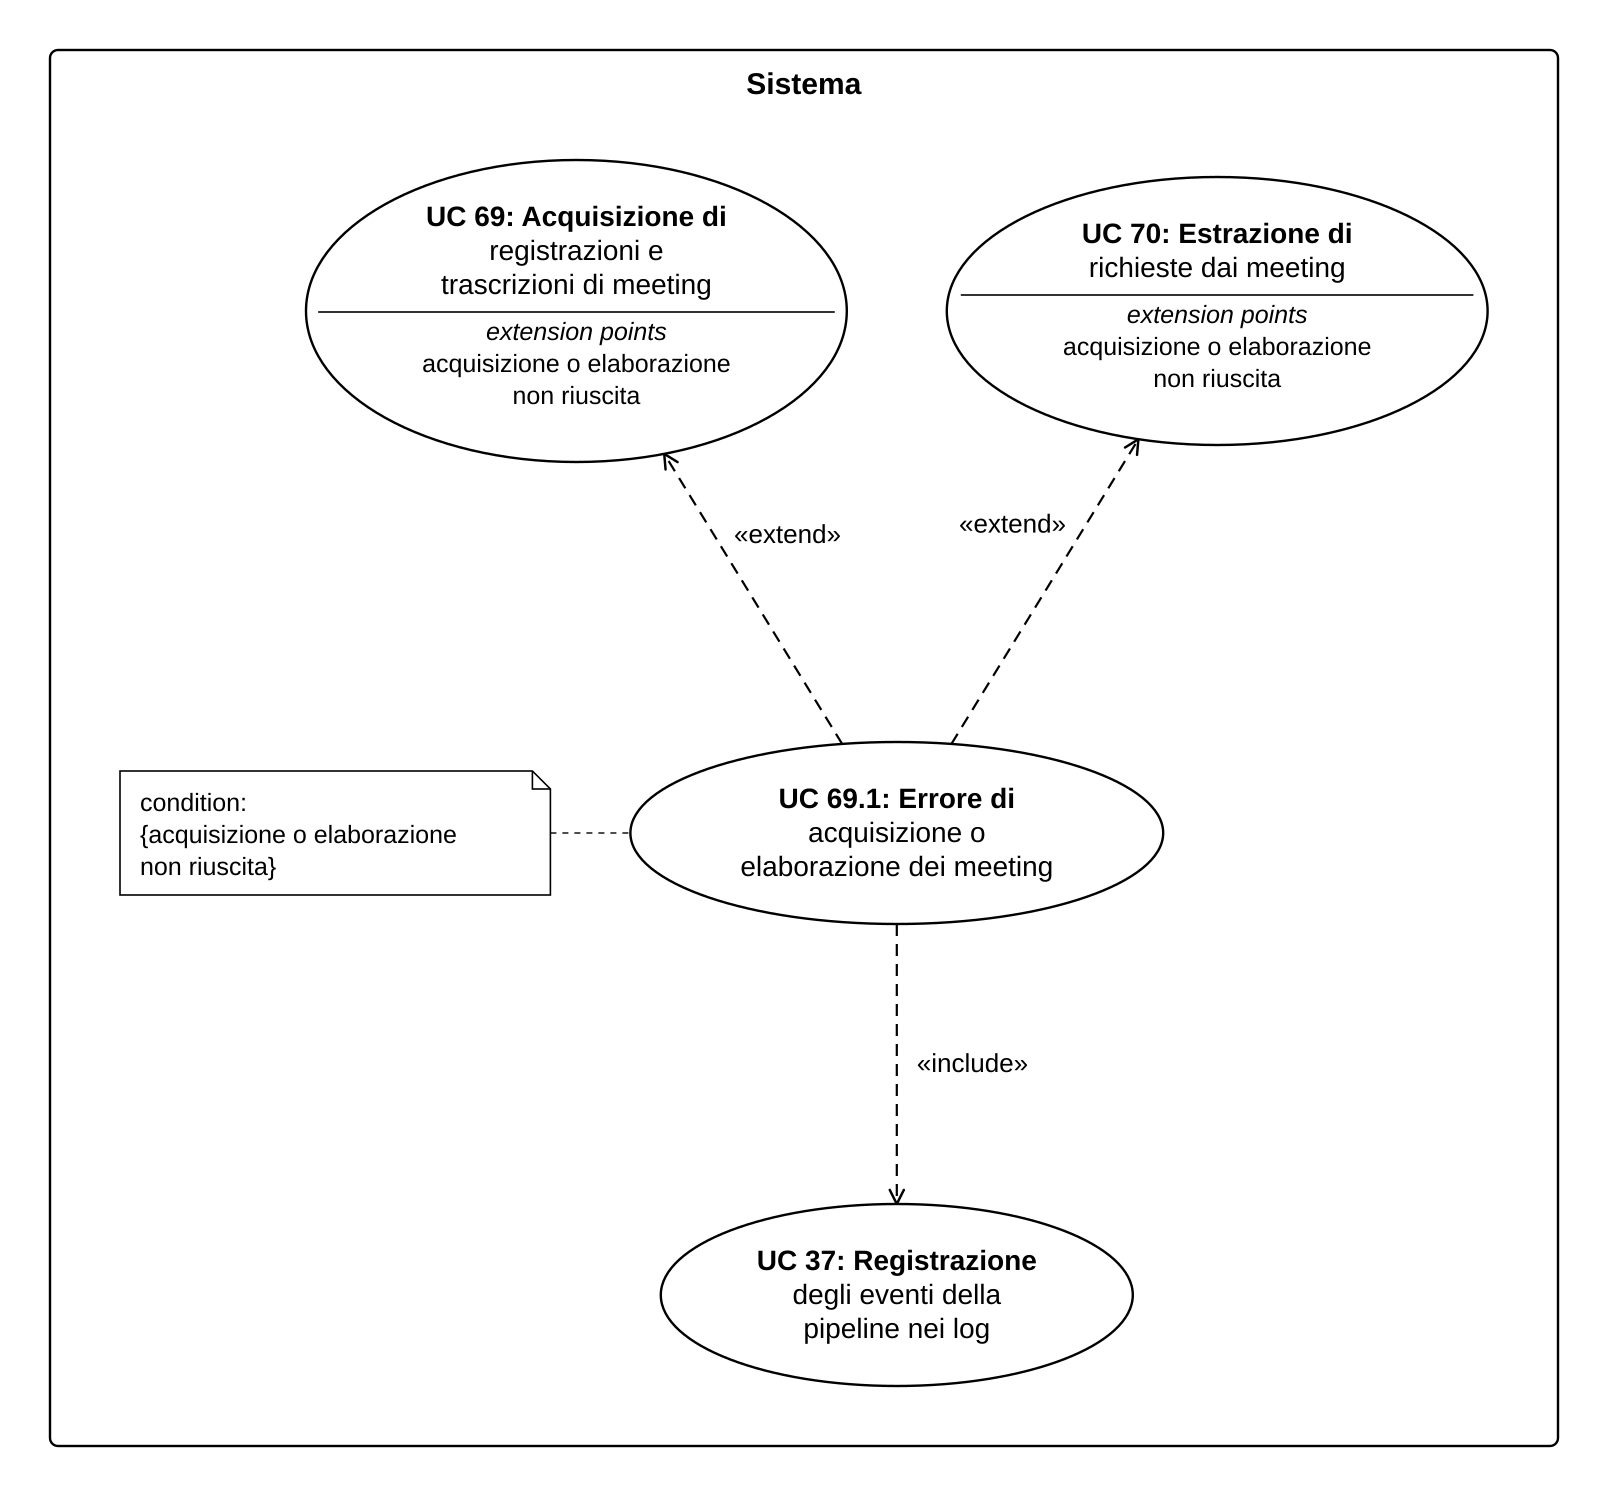
\includegraphics[width=\linewidth,height=0.32\textheight,keepaspectratio]{img/UC69_1.png}
\caption{UC 69.1 -- Errore di acquisizione o elaborazione dei meeting}
\end{center}
\begin{itemize}
    \item \textbf{Attore principale}: Mittente
    \item \textbf{Precondizioni}: L'acquisizione o l'elaborazione di un meeting è in corso.
    \item \textbf{Scenario principale}:
    \begin{enumerate}
        \item Il sistema rileva un errore.
        \item Il sistema registra l'errore nei log (\hyperref[uc:37]{UC 37}).
    \end{enumerate}
    \item \textbf{Postcondizioni}: L'errore è registrato nei log.
    \item \textbf{Trigger}: Acquisizione o elaborazione non riuscita.
    \item \textbf{Estende}: \hyperref[uc:69]{UC 69}, \hyperref[uc:70]{UC 70}.
    \item \textbf{Inclusioni}:
    \begin{itemize}
        \item \hyperref[uc:37]{UC 37}: Registrazione degli eventi della pipeline nei log
    \end{itemize}
\end{itemize}

\subsubsection{UC 70: Estrazione di richieste dai meeting}\label{uc:70}
\begin{center}
\captionsetup{type=figure}
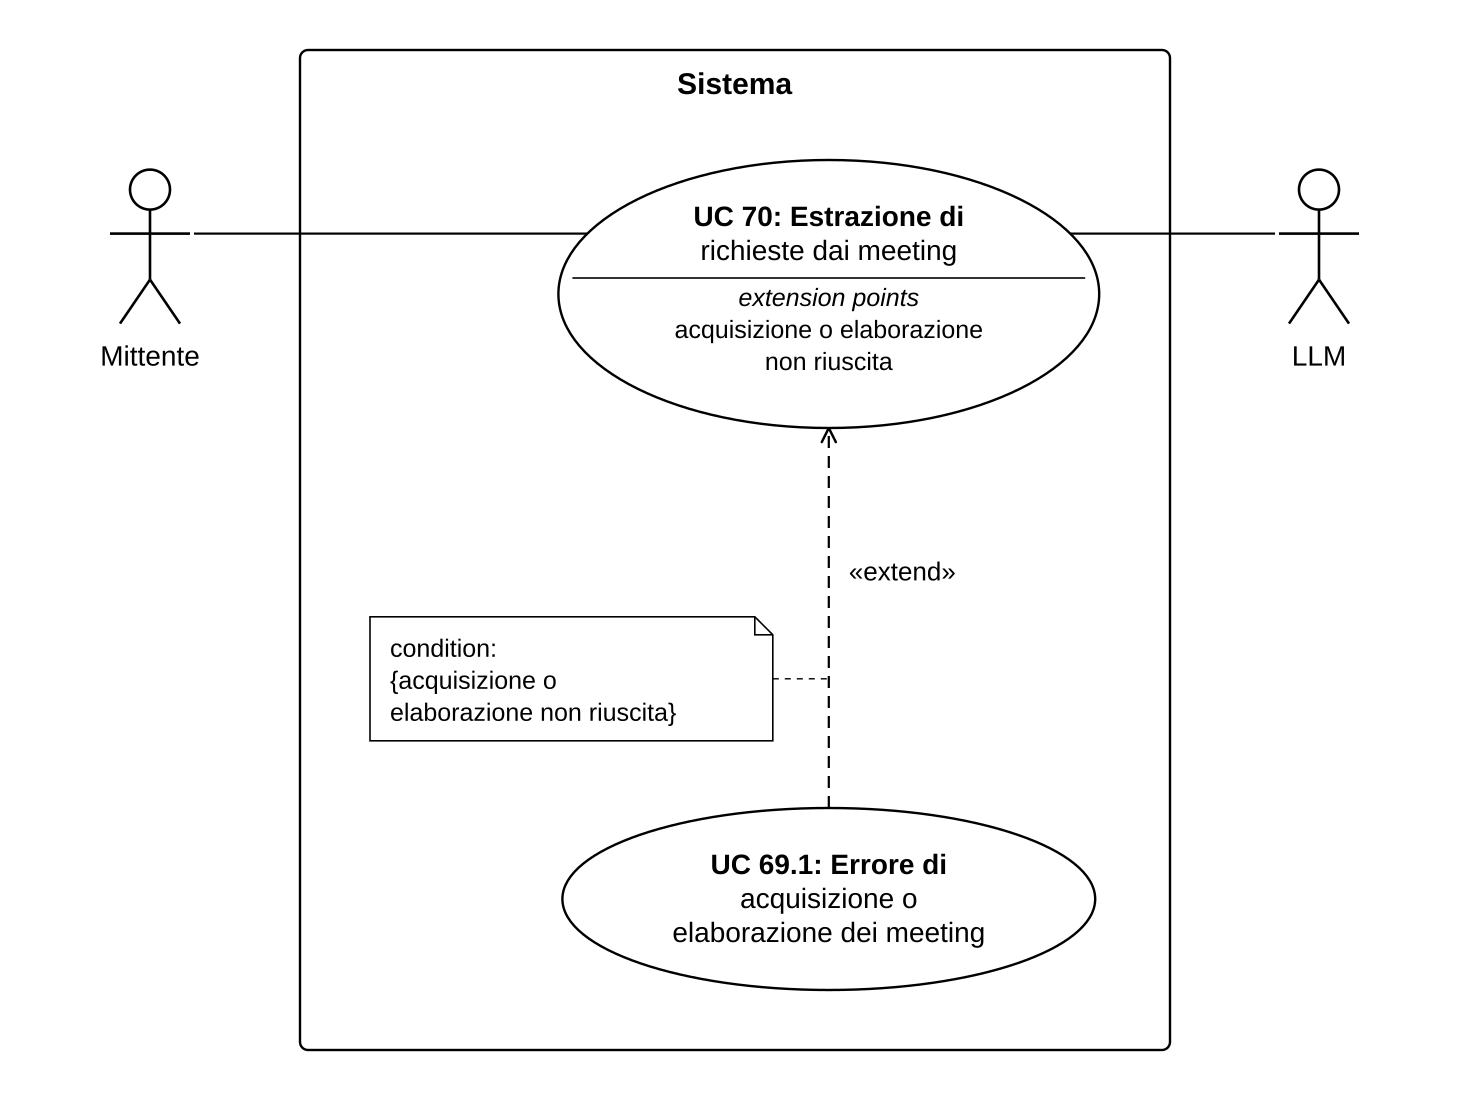
\includegraphics[width=\linewidth,height=0.32\textheight,keepaspectratio]{img/UC70.png}
\caption{UC 70 -- Estrazione di richieste dai meeting}
\end{center}
\begin{itemize}
    \item \textbf{Attore principale}: Mittente
    \item \textbf{Attori secondari}: LLM
    \item \textbf{Precondizioni}: Un meeting è stato acquisito e il servizio LLM è raggiungibile.
    \item \textbf{Scenario principale}:
    \begin{enumerate}
        \item Il sistema invia il contenuto all'LLM con contesto complessivo.
        \item L'LLM estrae ordini, ticket e richieste di assistenza.
        \item Il sistema crea le richieste corrispondenti.
    \end{enumerate}
    \item \textbf{Postcondizioni}: Le richieste del meeting sono estratte.
    \item \textbf{Trigger}: Meeting acquisito.
    \item \textbf{Estensioni}:
    \begin{itemize}
        \item \hyperref[uc:69.1]{UC 69.1}: Errore di acquisizione o elaborazione dei meeting $\rightarrow$ Condizione: Acquisizione o elaborazione non riuscita.
    \end{itemize}
\end{itemize}